% Copyright (C) 2024 Songbingzhi628. This work is licensed under Creative Commons Attribution-NonCommercial-ShareAlike 4.0 International License.
% Email: 13012057210@163.com

\ChDecl{Ch1B}{1$\cdot$B}{}

\vspace{2pt}

\ProblemN{\Anchor{1B1}{1}}{
	\vspace{2pt}\TextA{Prove $\forall v\in V,-\Par{{-v}} = v$.}
}$-\Par{{-v}}=\Par{{-1}}\BigPar{\Par{{-1}}v}=\BigPar{\Par{{-1}}\Par{{-1}}}v=1\cdot v=v.$\parSol{\vspace{4pt}}
\Or Becs $-\Par{{-v}}+\Par{{-v}}=0$ 又 $v+\Par{{-v}}=0.$ Now by the uniqnes of add inv.\PfEnd
\SepLine

\ProblemN{\Anchor{1B2}{2}}{
	\TextA{Supp $a\in\Fbb,v\in V$, and $av = 0$. Prove $a = 0$ or $v = 0$.}
}Supp $a\neq 0,\,\exists\,a^{-1}\in\Fbb,\,a^{-1}a=1,$ hence $v=1\cdot v=\Par{a^{-1}a}v=a^{-1}\Par{av}=a^{-1}\cdot 0=0.$\PfEnd
\SepLine

\ProblemN{\Anchor{1B3}{3}}{
	\TextA{Supp $v, w\in V$. Explain why $\exists\,!\,x\in V,v + 3x = w.$}
}$v + 3x = w \;\Leftrightarrow\; 3x = w − v \;\Leftrightarrow\; x = \frac{\;1\;}{3}\Par{w-v}.$\PfEnd\vspace{4pt}\quad
\Or \hspace{1pt}\;{\Existns} \;Let $x=\Frac{\;1\;}{3}\Par{w-v}.$\vspace{2pt}\par\quad
\Blind{\Or}{\Uniqnes} \;If $v+3x_1=w,$(I)$\,\,v+3x_2=w\,$(II). Then (I) $-$ (II) $: 3\Par{x_1-x_2}=0\Rightarrow x_1=x_2.$\PfEnd
\SepLine

\Anchor{1B5}\ProblemN{5}{
	\TextA{Show in the def of a vecsp, the add inv cond can be replaced by [1.29].}
	\TextA{\large{\tgsc Hint\tgbf:} Supp $V$ satisfies all conds in the def, except we've replaced the add inv cond with [1.29].}
	\TextA{\large\Blind{{\tgsc Hint\tgbf:}} Prove the add inv is true.}
}Using [1.31]. $0v=0\Longleftrightarrow\Sbra{1+\Par{{-1}}}v=1\cdot v+\Par{{-1}}v=v+\Par{{-v}}=0.$\PfEnd
%\Blind{\IndentN} \AComm Becs $\forall v\in V,v+\Par{{-1}}v=0v=0\Rightarrow\exists\,w=\Par{{-1}}v\in V,v+w=0.$\par
%\Blind{\IndentN} \IndentComment{}The add inv cond can also be replaced by [1.31].
\SepLine

\ProblemN{\Anchor{1B6}{6}}{
	\TextA{Let $\infty$ and $-\infty$ denote two disti objects that are not in $\Rbb$.}
	\TextA{Define the natural add and scalar multi on $\Rbb\cup\Bra{\infty, -\infty},$ that is, for each $t\in\Rbb,$\vspace{4pt}}
	\TextA{\;\FontNorm$t\infty=\hMath{l}{\left\{}{\;\right|}{
		-\infty\,$ if $t<0,\\
		\Blind{-}0\,$\,\, if $t=0,\\
		\hfill\infty\,\,\,$if $t>0,}\,\,\,t\Par{{-\infty}}=\hMath{l}{\left\{}{\;\right|}{
		-\infty\,$ if $t>0,\\
		\Blind{-}0\,$\,\, if $t=0,\\
		\hfill\infty\,\,\,$if $t<0,}$\tgnr$\:\hText{$
		(a) $t + \infty = \infty + t = \infty + \infty = \infty,\\$
		(b) $t + \Par{{-\infty}} = \Par{{-\infty}} + t = \Par{{-\infty}} + \Par{{-\infty}} = -\infty,\\$
		(c) $\infty + \Par{{-\infty}} = \Par{{-\infty}} + \infty = 0.}$\vspace{4pt}}
	\TextA{Is $\Rbb\cup\Bra{\infty, -\infty}$ a vecsp over $\Rbb$? Explain.}
}No. Becs the add and scalar multi is not assoc and distr.\parSol{}
By Assoc: $\Par{a+\infty}+\Par{{-\infty}}\neq a+\Par{\infty+\Par{{-\infty}}}.$\parSol{}
\Or By Distr: $\infty=\Par{2+\Par{{-1}}}\infty\neq 2\infty+\Par{{-\infty}}=\infty+\Par{{-\infty}}=0.$\PfEnd
\SepLine

\Anchor{1BN1}\ProblemBX[]{\NoteFor{Fields}}{
	\TextB{Many choices.\;\;\FontNorm\Sbra[3pt]{{\tgsl Req Multi Inv Uniq}}\vspace{2pt}}
	\TextB{\AExa $\Zbb_m=\Bra{K_0,K_1,\dots,K_{m-1}}$ is a field $\Longleftrightarrow m\in\Nbp$ is a prime.}
}\SepLine

%\ProblemB{
%	\TextB{Let $\mS$ be the collec of all subsets of $\Fbb.$ Define the add and scalar multi on $\mS$ by}
%	\TextB{$A+B=\Bra{a+b:a\in A,b\in B},\lambda A=\Bra{\lambda a:a\in A},$ and $A+\emptySet=\emptySet=A,\lambda\emptySet=\emptySet.$}
%	\TextB{Is $\mS$ a vecsp over $\Fbb$? Which req in [1.19] does $\mS$ not hold ?}
%}
%\SepLine

\ChEnd

\pagebreak

\ChDecl{Ch1C}{1$\cdot$C}{\quad{\small\textbf{注意\,:}\;这里我将3.E积空间的定义前置;仅涉及概念。}}

\vspace{2pt}

\Anchor{1CNE5}\BulletPointX\NoteForSmall{Exe (5)}\;\;$\Cbb=\Rbb\oplus\Bra{c\i:c\in\Rbb}=\Bra{a+b\i:a,b\in\Rbb}$ if we let $\Fbb=\Rbb$ and $\i^2=-1.$\vspace{-4pt}
\SepLine

\Anchor{1CNE6}\BulletPointX\NoteForSmall{Exe (6)}\;\;Supp $V$ is a vecsp over $\Rbb.$ Then $V$ is not a vecsp over $\Cbb.$ See also (9.A.16,17).\par
\BulletPointX\AComm Supp $V$ is a vecsp over $\Cbb$ of dim $n.$ Then $V$ is also a vecsp over $\Rbb$ of dim $2n.$\vspace{-4pt}
\SepLine

\ProblemN[]{\Anchor{1C7}\Anchor{1C8}{7, 8}}{
	\TextA{Give a non-trivial $U\subseteq\Rbb^2,$ $U$ is}
	\PrePa\TextA{closd taking add invs and add, but is not a subsp of $\Rbb^2.$\hfill\tgnr\FontNorm Let $U=\Zbb^2$ or $\Qbb^2,$ with $0\in U.$}
	\PrePb\TextA{scalar multi, but is not a subsp of $\Rbb^2.$\hfill\tgnr\FontNorm Let $U=\Bra{\Par{x,y}\in\Rbb^2:x=0\vee y=0}.$}
}\SepLine

\BulletPointX\Largesl{Supp $U,W,V_{\!1},V_{\!2},V_{\!3}$ are subsps of $V.$}\par
\Anchor{1C15}\Anchor{1C16}\Onumber{15}\quad{$U+U\ni u+w\in U.$} \qquad \Onumber{16}\quad{$U+W\ni u+w=w+u\in W+U.$}\PfEnd
\Onumber{\Anchor{1C17}{17}}\quad{$\Par{V_{\!1}+V_{\!2}}+V_{\!3}\ni\Par{v_1+v_2}+v_3=v_1+\Par{v_2+v_3}\in V_{\!1}+\Par{V_{\!2}+V_{\!3}}.$}\PfEnd\Anchor{1C'1}
\BulletPointX{ \quad}{$\Par{U+W}{_{\Cbb}}\ni \Par{u_1+w_1}+\i\Par{u_2+w_2}=\Par{u_1+\i u_2}+\Par{w_1+\i w_2}\in U_\Cbb+W_{\!\Cbb}.$}\PfEnd
\BulletPointX{ \quad}$\Par{U\cap W}{_\Cbb}\ni u_1+\i u_2=w_1+\i w_2\in U_\Cbb\cap W_\Cbb.$\PfEnd
\BulletPointX{ \quad}$U_\Cbb=W_\Cbb\Longleftrightarrow U=W.$ \;Supp $U_\Cbb\ni u+\i v\in W_\Cbb.$ Then $U\ni u,v\in W.$\PfEnd
\SepLine


\ProblemN{\Anchor{1C18}{18}}{
	\TextA{Does the add on the subsps of $V$ have an add id? Which subsps have add invs?}
}Supp $\Omega$ is the uniq add id.\par\quad
(a) For any subsp $U$ of $V,$ $\Omega\subseteq U+\Omega=U\Rightarrow\Omega\subseteq U$. Let $U=\zeroSubs,$ then $\Omega=\zeroSubs.$\par\quad
(b) Supp $U+W=\Omega.$ Becs $U+W\supseteq U,W\Rightarrow \Omega\supseteq U,W\Rightarrow U=W=\Omega=\zeroSubs.$\PfEnd
\SepLine

\ProblemN{\Anchor{1C11}{11}}{
	\TextA{Prove the intersec of every collec of subsps of $V$ is a subsp of $V$.}
}Supp $\Bra{U_{\alpha}}{_{\alpha\in\Gamma}}$ is a collec of subsps of $V$; here $\Gamma$ is an index set.\vspace{2pt}\parSol{}
We show $\bigcap_{\alpha\in\Gamma}U_\alpha,$ which equals the set of vecs in each $U_\alpha,$ is a subsp of $V$.\vspace{2pt}\parSol{}
(a) $0\in\bigcap_{\alpha\in\Gamma}U_\alpha.$ Nonempty.\parSol{}
(b) $u,v\in\bigcap_{\alpha\in\Gamma}U_\alpha\Rightarrow u+v\in U_\alpha,\,\,\forall\alpha\in\Gamma\Rightarrow u+v\in\bigcap_{\alpha\in\Gamma}U_\alpha$. Closd add.\parSol{}
(c) $u\in\bigcap_{\alpha\in\Gamma}U_\alpha,\lambda\in\Fbb\Rightarrow\lambda u\in U_\alpha,\,\,\forall\alpha\in\Gamma\Rightarrow\lambda u\in\bigcap_{\alpha\in\Gamma}U_\alpha$. Closd scalar multi.\vspace{4pt}\parSol{}
Thus $\bigcap_{\alpha\in\Gamma}U_\alpha$ is nonempty subset of $V$ that is closd add and scalar multi.\PfEnd
\SepLine

\Anchor{1CN1.45}\BulletPointX\NoteForSmall{[1.45]}\;\;Another proof: Supp $\forall v\in V,\exists\,!\,\Par{u,w}\in U\times W,v=u+w.$\TextB{}
\Blind{\NoteForSmall{[1.45]}\;\;}Asum non0 $v\in U\cap W.$ Then the $\Par{u,w}=\Par{v,0}$ or $\Par{0,v},$ ctradic the uniqnes.\PfEnd\vspace{-2pt}
\SepLine

\Anchor{1CT1}\ProblemBX[]{\TipsN{1}}{
	Supp $U,W\subseteq V.$ And $U,W,V$ are vecsps $\Rightarrow U,W$ are subsps of $V.$\TextA{}
	Then $U+W$ is also a subsp of $V.$ Becs $\forall u\in U,w\in U,u+w\in V$ since $u,w\in V.$\TextA{\vspace{-3pt}}
}\SepLine

\Anchor{1CN1.38}\ProblemB{
	\TextB{Supp $U=\Bra{\Par{x,x,y,y}},W=\Bra{\Par{x,x,x,y}}\subseteq\Fbb^4.$ Prove $U+W=\Bra{\Par{x,x,y,z}}.$\vspace{2pt}}
}Let T denote $\Bra{\Par{x,x,y,z}}.$ By def, $U+W\subseteq T.$\par\quad
And $T\ni\Par{x,x,y,z}\Rightarrow\Par{0,0,y-x,y-x}+\Par{x,x,x,-y+x+z}\in U+W$. Hence $T\subseteq U+W.$\PfEnd
\SepLine

\ProblemN{\Anchor{1C21}{21}}{
	\TextA{Supp $U=\Bra{\Par{x,y,x+y,x-y,2x}}$. Find a $W$ suth $\Fbb^5=U\oplus W$.}
}Let $W=\Bra{\Par{0,0,z,w,u}}$. Then $U\cap W=\zeroSubs$.\parSol{}
And $\Fbb^5\ni\Par{x,y,z,w,u}\Rightarrow\Par{x,y,x+y,x-y,2x}+\Par{0,0,z-x-y,w-x-y,u-2x}\in U+W.$\par
\SepLine\pagebreak

\ProblemN{\Anchor{1C22}{22}}{
	\TextA{Supp $U=\Bra{\Par{x,y,x+y,x-y,2x}\in\Fbb^5}$.}
	\TextA{Find non0 subsps $W_1,W_2,W_3$ of $\,\Fbb^5$ suth $\Fbb^5 = U\oplus W_1\oplus W_2\oplus W_3 $.}\vspace{-2pt}
}\par\quad
Let $W_1=\Bra{\Par{0,0,z,0,0}\in\Fbb^5}\Rightarrow W_1\cap U=\zeroSubs.$ \hfill Now $U\oplus W_1=\Bra{\Par{x,y,z,x-y,2x}\in\Fbb^5}=U_1$.\par\quad
Let $W_2=\Bra{\Par{0,0,0,w,0}\in\Fbb^5}\Rightarrow W_2\cap U_1=\zeroSubs.$ \hfill Now $U_1\oplus W_2=\Bra{\Par{x,y,z,w,2x}\in\Fbb^5}=U_2$.\par\quad
Let $W_3=\Bra{\Par{0,0,0,0,u}\in\Fbb^5}\Rightarrow W_3\cap U_2=\zeroSubs.$ \hfill Now $U_2\oplus W_3=\Bra{\Par{x,y,z,w,u}\in\Fbb^5}=U_3$.\par\quad
Thus $\Fbb^5=\Sbra{\Par{U\oplus W_1}\oplus W_2}\oplus W_3.$\PfEnd
\SepLine

\ProblemN{\Anchor{1C23}{23}}{
	\TextA{Give an exa of vecsps $V_{\!1},V_{\!2},U$ suth $V_{\!1}\oplus U=V_{\!2}\oplus U$, but $V_{\!1}\neq V_{\!2}$.\vspace{0pt}}
}$V=\Fbb^2$,  $U=\Bra{\Par{x,x}}$, $V_{\!1}=\Bra{\Par{x,0}}$, $V_{\!2}=\Bra{\Par{0,x}}$.\par
\SepLine

\Anchor{1CNC}\BulletPointX\NoteForSmall{\Large $“\complement_V U \cup \zeroSubs”$}\;\;$“\complement_V U \cup \zeroSubs”$ is supposed to be a subsp $W$ suth $V=U\oplus W$.\TextB{\vspace{3pt}}
But if we let $u\in U\nonzero$ and $w\in W\nonzero$, then $\MathRightBrace{l}{w\in\complement_V U \cup \zeroSubs\\ u\pm w\in\complement_V U \cup \zeroSubs }\Rightarrow u\in\complement_V U \cup \zeroSubs.$ Ctradic.\vspace{3pt}\TextB{}
To fix this, {\FontLarge denote the set $\Bra{W_{\hspace{-1pt}1},W_{\hspace{-1pt}2},\cdots}$ by $\Scom{V}{U}$,} {\small where each $W_{\!i}\oplus U=V.$}
\SepLine

\Anchor{1CT2}\ProblemBX{\TipsN{2}}{
	\TextA{Supp $V_{\!1}\subseteq V_{\!2}$ in Exe {\tgnr(23)}. Prove $V_{\!1}=V_{\!2}.$}
}Becs the subset $V_{\!1}$ of vecsp $V_{\!2}$ is closd add and scalar multi, $V_{\!1}$ is a subspace of $V_{\!2}.$\parSol{}
Supp $W$ is suth $V_{\!2}=V_{\!1}\oplus W.$ Now $V_{\!2}\oplus U=\Par{V_{\!1}\oplus W}\oplus U=\Par{V_{\!1}\oplus U}\oplus W=V_{\!1}\oplus U.$\parSol{}
If $W\neq\zeroSubs,$ then $V_{\!1}\oplus U\subsetneq\Par{V_{\!1}\oplus U}\oplus W$, ctradic. Hence $W=\zeroSubs,V_{\!1}=V_{\!2}.$\PfEnd
\SepLine

\Anchor{1C'2}\ProblemB{
	\TextB{Supp $V_{\!1},V_{\!2},U_1,U_2$ are vecsps, $V_{\!1}\oplus U_1=V_{\!2}\oplus U_2,\;V_{\!1}\subseteq V_{\!2},\;U_2\subseteq U_1.$}
	\TextB{Prove or give a countexa\hspace{1pt}$:$ $V_{\!1}=V_{\!2},\;U_1=U_2.$}
}Let $U_2=\zeroSubs.$ Give an exa that each of $V_{\!1},V_{\!2},U_1$ is non0.\par\vspace{-58pt}\quad
\hspace{450pt}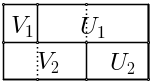
\includegraphics[width=2.4cm,height=1.2cm,scale=0.22]{diagram1C-1.png}\vspace{18pt}\PfEnd
\SepLine

\ProblemB{
	\TextA{Supp the intersec of any two of the vecsps $U,W,X,Y$ is $\zeroSubs.$}
	\TextA{Give an exa that $\BigPar{X\oplus U}\,${\LARGE$\cap$}$\,\BigPar{Y\oplus W}\neq\zeroSubs.$}
}\Sbra{ Using notas in Chapter 2. } \;Let $B_X=\Par{e_1},B_U=\Par{e_2-e_1},B_Y=\Par{\,},B_W=\Par{e_2}.$
\SepLine

\Anchor{1CT3}\ProblemBX{\TipsN{3}}{
	\TextA{Supp $V=X\oplus Y,$ and $Z$ is a subsp of $V.$ Show $X\subseteq Z\Rightarrow Z=X\oplus\Par{Y\cap Z}.$}
}$\forall z\in Z,\exists\,!\,\Par{x,y}\in X\times Y,\,z=x+y.$\parSol{}
Becs $x\in Z\Rightarrow z-x=y\in Z\Rightarrow z\in X+\Par{Y\cap Z}.$ 又 $X\cap\Par{Y\cap Z}\subseteq X\cap Y.$\PfEnd
\SepLine

\Anchor{1CT4}\ProblemBX{\TipsN{4}}{
	\TextA{Let $V=U+W,\;I=U\cap W,\,U=I\oplus X,\,W=I\oplus Y.$ Prove $V=I\oplus\Par{X\oplus Y}.$}
}We show $X\cap Y=U\cap Y=W\cap X=\zeroSubs$ by ctradic.\parSol{}
$X\cap Y=\Delta\neq\zeroSubs\Rightarrow I=U\cap W\supseteq\Delta\Rightarrow I\cap X\neq\zeroSubs, I\cap Y\neq\zeroSubs.$\parSol{}
$U\cap Y=\Delta\neq\zeroSubs\Rightarrow I=U\cap W\supseteq\Delta\Rightarrow I\cap Y\neq\zeroSubs.$ Simlr for $W\cap X.$\parSol{\vspace{2pt}}
Thus $I+\Par{X+Y}=\Par{I\oplus X}\oplus Y=I\oplus\Par{X\oplus Y}.$\parSol{\vspace{2pt}}
Now we show $V=I+\Par{X+Y}.$ \;$\forall v\in V,v=u+w,\exists\,\Par{u,w}\in U\times W$\parSol{}
$\Rightarrow\exists\,\Par{i_u,x_u}\in I\times X,\,\Par{i_w,y_w}\in I\times Y,\;v=\Par{i_u+i_w}+x_u+y_w\in I+\Par{X+Y}.$\PfEnd
\SepLine\pagebreak

\ProblemN{\Anchor{1C12}{12}}{
	\TextA{Supp $U,W$ are subsps of $V.$ Prove $U\cup W$ is a subsp of $V\Longleftrightarrow U\subseteq W$ or $W\subseteq U$.}
}(a) Supp $U\subseteq W$. Then $U\cup W=W$ is a subsp of $V$.\parSol{}
(b) Supp $U\cup W$ is a subsp of $V$. Asum $U\not\subseteq W,\;U\not\supseteq W$ \BigPar{ $U\cup W\neq U$ and $W$ }.\parSol{\Hb}
Then $\forall a\in U\wedge a\not\in W,\forall b\in W\wedge b\not\in U,$ we have $a+b\in U\cup W$.\parSol{\vspace{2pt}\Hb}
\!\!\!$\MathRightMid{l}{$
$a+b\in U\Rightarrow b=\Par{a+b}+\Par{{-a}}\in U$, ctradic $\Rightarrow W\subseteq U.\\ $
$a+b\in W\Rightarrow a=\Par{a+b}+\Par{{-b}}\in W$, ctradic $\Rightarrow U\subseteq W.}\hText{$
Ctradic asum.$\\\;}$\PfEnd[-14pt]
\SepLine

\ProblemN{\Anchor{1C13}{13}}{
	\TextA{Supp $U_1,U_2,U_3$ are subsps of $V,$ and the union $U_1\cup U_2\cup U_3=\mathcal{U}$ is a subsp of $V.$}
	\TextA{Prove one of the subsps contains the other two.}
	\TextA{\large This exe is not true if we \uline{replace $\Fbb$ with a field containing only two elems.}}
}\uline{\AExa Let $\Fbb=\Zbb_2.$} $U_1=\Bra{u,0},U_2=\Bra{v,0},U_3=\Bra{v+u,0}.$ While $\mathcal{U}=\Bra{0,u,v,v+u}$ is a subsp.\vspace{4pt}\par\quad
\NOTICE that, $U\cup W=V$ is vecsp $\notRightarrow U,W$ are subsps of $V.$\par\quad
This trick is invalid: $\Par{A\cup B}\cup\Par{B\cup C}=\Par{A\cup C}\cup\Par{B\cup C}=\Par{A\cup B}\cup\Par{A\cup C}.$\vspace{2pt}\par\quad
(I) If any $U_j$ is contained in the union of the other two, say $U_1\subseteq U_2\cup U_3,$ then $\mathcal{U}=U_2\cup U_3.$\par\quad\HI
By applying Exe (12) we conclude that one $U_j$ contains the other two. Thus done.\vspace{2pt}\par\quad\EndI
(II) \envFontLarge{Asum no one is contained in the union of other two, and no one contains the other two.}\par\quad\HII
{\vspace{4pt}Say $U_1\not\subseteq U_2\cup U_3$ and $U_1\not\supseteq U_2\cup U_3.$}\par\quad
{\Large\vspace{4pt}$\exists\,u\in U_1\wedge u\not\in U_2\cup U_3;\;v\in U_2\cup U_3\wedge v\not\in U_1.$ Let $W=\Bra{v+\lambda u:\lambda\in\Fbb}\,\subseteq\mathcal{U}.$}\par\quad
{\Large\vspace{4pt}Note that $W\cap U_1=\emptySet,$ for if any $v+\lambda u\in W\cap U_1$ then $v+\lambda u-\lambda u=v\in U_1$.}\par\quad
{\Large\vspace{4pt}Now $W\subseteq U_1\cup U_2\cup U_3\Rightarrow W\subseteq U_2\cup U_3.$ $\forall v+\lambda u\in W,v+\lambda u\in U_i,i=2,3.$}\par\quad
{\Large\vspace{4pt}If $U_2\subseteq U_3$ or $U_2\supseteq U_3,$ then $\mathcal{U}=U_1\cup U_i,i=2,3.$} {By Exe (12) done.}\par\quad
{\Large\vspace{4pt}Othws, {\FontNorm both $U_2,U_3\neq\zeroSubs.$} Becs \tgsl$W\subseteq U_2\cup U_3$ has at least three disti elems.}\par\quad
{\Large\vspace{4pt}There must be some $U_i$ that contains at least two disti elems of $W.$}\par\quad
{\Large$\exists\,\lambda_1\neq\lambda_2,\;v+\lambda_1 u$ \,and \,$v+\lambda_2 u$ \,both in $U_2$ or $U_3\Rightarrow u\in U_2\cap U_3,$ ctradic.}\FontNorm\PfEnd
\SepLine

\ChEnd\pagebreak

\ChDecl{Ch2A}{2$\cdot$A}{}

\vspace{6pt}

\ProblemN{\Anchor{2A1}{1}}{
	\TextA{Prove [P] $\Par{v_1,v_2,v_3,v_4}$ spans $V\Longleftrightarrow\BigPar{v_1-v_2,v_2-v_3,v_3-v_4,v_4}$ also spans V [Q].}
}Note that $V=\Span{v_1,\dots,v_n}\Longleftrightarrow\forall v\in V,\exists\,a_1,\dots,a_n\in\Fbb,v=a_1v_1+\dots+a_nv_n.$\par\quad
Asum $\forall v\in V,\exists\,a_1,\dots,a_4,b_1,\dots,b_4\in\Fbb,$ \BigPar{ that is, if $\exists\,a_i,$ then we are to find $b_i,$ vice versa }\par\quad
$v=a_1 v_1+a_2 v_2+a_3 v_3+a_4 v_4=b_1\Par{v_1-v_2}+b_2\Par{v_2-v_3}+b_3\Par{v_3-v_4}+b_4 v_4$\par\quad
$\Blind{v}=b_1 v_1+\Par{b_2-b_1}v_2+\Par{b_3-b_2}v_3+\Par{b_4-b_3}v_4$\par\quad
$\Blind{v}=a_1\Par{v_1-v_2}+\Par{a_1+a_2}\Par{v_2-v_3}+\Par{a_1+a_2+a_3}\Par{v_3-v_4}+\Par{a_1+\dots+a_4}v_4.$\PfEnd
\SepLine

\Anchor{2A4e3}\Anchor{2A4e14}\ProblemBnoor{4E 3, 14}{
	\TextB{Supp $\Par{v_1,\dots,v_m}$ is a list in $V$. For each $k$, let $w_k=v_1+\dots+v_k$.}
	(a) \TextB{Show $\Span{v_1,\dots,v_m}=\Span{w_1,\dots,w_m}.$}
	(b) \TextB{Show [P] $\Par{v_1,\dots,v_m}$ is liney indep $\Longleftrightarrow$ $\Par{w_1,\dots,w_m}$ is liney indep [Q].}
}\par\quad
(a) Asum $a_1v_1+\dots+a_mv_m=b_1w_1+\dots+b_mw_m=b_1v_1+\dots+b_k\Par{v_1+\dots+v_k}+\dots+b_m\Par{v_1+\dots+v_m}.$\par\quad\Ha
Then $a_k=b_k+\dots+b_m;\;\;a_{k+1}=b_{k+1}+\dots+b_m\Rightarrow b_k=a_k-a_{k+1};\;b_m=a_m.$ Simlr to Exe (1).\vspace{4pt}\par\quad
(b) $P\Rightarrow Q:\;\;b_1 w_1+\dots+b_m w_m=0=a_1 v_1+\dots+a_m v_m,\text{\;where\;}0=a_k=b_k+\dots+b_m.$\par\quad\Hb
$Q\Rightarrow P:\;\;a_1 v_1+\dots+a_m v_m=0=b_1 w_1+\dots+b_m w_m=0, \text{\;where\;} 0=b_m=a_m,\;0=b_k=a_k-a_{k+1}.$\vspace{4pt}\par\quad\Hb
\Or By (a), let $W=\Span{v_1,\dots,v_m}=\Span{w_1,\dots,w_m}.$ Supp $\Par{v_1,\dots,v_m}$ is liney dep.\par\quad\Hb
By [2.21](b), a list of len $\Par{m-1}$ spans $W.$ 又 By [2.23], $\Par{w_1,\dots,w_m}$ liney indep $\Rightarrow m\leqslant m-1.$\par\quad\Hb
Thus $\Par{w_1,\dots,w_m}$ is liney dep. Now rev the roles of $v$ and $w.$\PfEnd
\SepLine

\ProblemN{\Anchor{2A2}{2}}{
	(a) \TextA{[P]\hspace{17pt}{\; A list $\Par{v}$ of len $1$ in $V$ is liney indep $\Longleftrightarrow v\neq 0.$} \hfill[Q]}
	(b) \TextA{[P]{\; A list $\Par{v,w}$ of len $2$ in $V$ is liney indep $\Longleftrightarrow\forall\lambda,\mu\in\Fbb,v\neq \lambda w,w\neq \mu v.$} \hfill[Q]\vspace{4pt}}
}(a) $Q\Rightarrow P:$ $v\neq 0\Rightarrow$ if $av=0$ then $a=0\Rightarrow\Par{v}$ liney indep.\parSol{\Ha}
$P\Rightarrow Q:$ $\Par{v}$ liney indep $\Rightarrow v\neq 0$, for if $v=0,$ then $av=0\notRightarrow a=0.$\parSol{\Ha}
${}^\neg Q\Rightarrow{}^\neg P:$ $v=0\Rightarrow av=0$ while we can let $a\neq 0\Rightarrow\Par{v}$ is liney dep.\parSol{\Ha}
${}^\neg P\Rightarrow{}^\neg Q:$ $\Par{v}$ liney dep $\Rightarrow av=0$ while $a\neq 0\Rightarrow v=0.$\parSol{\vspace{4pt}}
(b) $P\Rightarrow Q:$ $\Par{v,w}$ liney indep $\Rightarrow$  if $av+bw=0,$ then $a=b=0\Rightarrow$ no scalar multi.\parSol{\Hb}
$Q\Rightarrow P:$ no scalar multi $\Rightarrow$ if $av+bw=0,$ then $a=b=0\Rightarrow\Par{v,w}$ liney indep.\parSol{\Hb}
${}^\neg P\Rightarrow{}^\neg Q:$ $\Par{v,w}$ liney dep $\Rightarrow$ if $av+bw=0,$ then $a$ or $b\neq 0\Rightarrow$ scalar multi.\parSol{\Hb}
${}^\neg Q\Rightarrow{}^\neg P:$ scalar multi $\Rightarrow$ if $av+bw=0,$ then $a$ or $b\neq 0\Rightarrow$ liney dep.\PfEnd
\SepLine

\ProblemN{\Anchor{2A10}{10}}{
	\TextA{Supp $\Par{v_1,\dots,v_m}$ is liney indep in $V$ and $w\in V$.}
	\TextA{Prove if $\BigPar{v_1+w,\dots,v_m+w}$ is linely dep, then $w\in\Span{v_1,\dots,v_m}$.}
}\par\quad
Note that $a_1\Par{v_1+w}+\dots+a_m\Par{v_m+w}=0\Rightarrow a_1 v_1+\dots+a_m v_m=-\Par{a_1+\dots+a_m}w.$\par\quad
Then $a_1+\dots+a_m\neq 0$, for if not, $a_1 v_1+\dots+a_m v_m=0$ while $a_i\neq 0$ for some $i$, ctradic.\par\quad
\Or We prove the ctrapos: Supp $w\not\in\Span{v_1,\dots,v_m}.$ Then $a_1+\dots+a_m=0.$\par\quad
Thus $a_1v_1+\dots+a_mv_m=0\Rightarrow a_1=\dots=a_m=0.$ Hence $\BigPar{v_1+w,\dots,v_m+w}$ is liney indep.\PfEnd\vspace{2pt}\quad
\Or $\exists\,j\in\Bra{1,\dots,m},v_j+w\in\Span{v_1+w,\dots,v_{j-1}+w}.$ If $j=1$ then $v_1+w=0$ and done.\par\quad
If $j\geqslant 2,$ then $\exists\,a_i\in\Fbb,v_j+w=a_1\Par{v_1+w}+\dots+a_{j-1}\Par{v_{j-1}+w}\Longleftrightarrow v_j+\lambda w=a_1 v_1+\dots+a_{j-1}v_{j-1}.$\par\quad
Where $\lambda=1-\Par{a_1+\dots+a_{j-1}}.$ Note that $\lambda\neq 0,$ for if not, $v_j+\lambda w=v_j\in\Span{v_1,\dots,v_{j-1}},$ ctradic.\par\quad
Now $w=\lambda^{-1}\Par{a_1 v_1+\dots+a_{j-1}v_{j-1}-v_j}\Rightarrow w\in\Span{v_1,\dots,v_m}.$\PfEnd
\SepLine

\ProblemN{\Anchor{2A11}{11}}{
	\TextA{Supp $\Par{v_1,\dots,v_m}$ is liney indep in $V$ and $w\in V$.}
	\TextA{Show [P] $\Par{v_1,\dots,v_m,w}$ is liney indep $\Longleftrightarrow w\not\in\Span{v_1,\dots,v_m}$ [Q].}
}Equiv to $\Par{v_1,\dots,v_m,w}$ liney dep $\Longleftrightarrow w\in\Span{v_1,\dots,v_m}.$ Using [2.21]. Obviously.\PfEnd
\ANote (a) Supp $\Par{v_1,\dots,v_m,w}$ is liney indep. Then $\Par{v_1,\dots,v_m}$ liney indep $\Longleftrightarrow w\not\in\Span{v_1,\dots,v_m}.$\parNot
(b) Supp $\Par{v_1,\dots,v_m,w}$ is liney dep. Then $\Par{v_1,\dots,v_m}$ liney indep $\Longleftrightarrow w\in\Span{v_1,\dots,v_m}.$
\SepLine

\ProblemN{\Anchor{2A14}{14}}{
	\TextA{Prove [P] $V$ is infinide $\Longleftrightarrow\exists$ seq $\Par{v_1,v_2,\dots}$ in $V$ suth each $\Par{v_1,\dots,v_m}$ liney indep. [Q]}
}$P\Rightarrow Q:\;$ Supp $V$ is infinide, so that no list spans $V.$ Define the desired seq recurly via:\parSol{}
\Blind{$P\Rightarrow Q:\;$} {\tgbf Step 1}\;\; Pick a $v_1\neq 0,\Par{v_1}$ liney indep.\parSol{}
\Blind{$P\Rightarrow Q:\;$} {\tgbf Step m}\; Pick a $v_m\not\in\Span{v_1,\dots,v_{m-1}},$ by Exe (11), $\Par{v_1,\dots,v_m}$ is liney indep.\vspace{4pt}\parSol{}
${}^\neg P\Rightarrow{}^\neg Q:\;$ Supp $V$ is finide and $V=\Span{w_1 , ..., w_m}$.\parSol{}
\Blind{${}^\neg P\Rightarrow{}^\neg Q:\;$} Let $\Par{v_1 , v_2 , \dots}$ be a seq in $V$, then $\Par{v_1,v_2,\dots,v_{m+1}}$ must be liney dep.\vspace{4pt}\parSol{}
\Or\; $Q\Rightarrow P:\;$ Supp there is such a seq.\parSol{}
\Blind{\Or\; $Q\Rightarrow P:\;$} Choose an $m$. Supp a liney indep list $\Par{v_1,\dots,v_m}$ spans $V$.\parSol{}
\Blind{\Or\; $Q\Rightarrow P:\;$} Simlr to [2.16]. $\exists\,v_{m+1}\in V\Backslash\Span{v_1,\dots,v_m}.$ Hence no list spans $V.$\PfEnd
\SepLine

\ProblemN{\Anchor{2A17}{17}}{
	\TextA{Prove $\Par{p_0,p_1,\dots,p_m}$ cannot be liney indep in $\PoF{m}$ with each $p_k\Par{2}=0.$}
}\par\quad
Supp $\Par{p_0,p_1,\dots,p_m}$ is liney indep. Define $p\in\PoF{m}$ by $p\Par{z}=z.$\par\quad
\NOTICE that $\forall a_i\in\Fbb,z\neq a_0 p_0\Par{z}+\dots+a_m p_m\Par{z},$ for if not, let $z=2.$ Thus $z\not\in\Span{p_0,p_1,\dots,p_m}$.\par\quad
Then $\Span{p_0,p_1,\dots,p_m}\subsetneq\PoF{m}$ while the list $\Par{p_0,p_1,\dots,p_m}$ has len $\Par{m+1}$.\par\quad
Hence $\Par{p_0,p_1,\dots,p_m}$ is linely dep. For if not, then becs $\Par{1,z,\dots,z^m}$ of len $\Par{m+1}$ spans $\PoF{m},$\par\quad
by the steps in [2.23] trivially, $\Par{p_0,p_1,\dots,p_m}$ of len $\Par{m+1}$ spans $\PoF{m}.$ Ctradic.\PfEnd\vspace{6pt}\par\quad
\Or Becs $\Par{1,z,\dots,z^m}$ of len $\Par{m+1}$ spans $\PoF{m}.$ Then $\Par{p_0,p_1,\dots,p_m,z}$ of len $\Par{m+2}$ is liney dep.\par\quad
As shown above,  $z\not\in\Span{p_0,p_1,\dots,p_m}.$ And hence by [2.21](a), $\Par{p_0,p_1,\dots,p_m}$ is liney dep.\PfEnd
\SepLine
\ChEnd

\vfill\ChDecl{Ch2B}{2$\cdot$B}{}

\vspace{4pt}

\Anchor{2BN2.34}\BulletPointX\NoteFor{{\tgsc liney indep seq and }[2.34]}\;\;$“V=\Span{v_1,\dots,v_n,\dots}”$ is an invalid expr.\TextB{}
If we allow using $“$infini list$”$, then we must assure that $\Par{v_1,\dots,v_n,\dots}$ is a spanning $“$list$”$\TextB{}
suth $\forall v\in V,\exists$ smallest $n\in\Nbp,\;v=a_1 v_1+\dots+a_n v_n.$ Moreover, given a list $\Par{w_1,\cdots,w_n,\cdots}$ in $W,$\TextB{}
we can prove $\exists\,!\,T\in\Lm{V,W}$ with each $Tv_k=w_k,$ which has less restr than [3.5].\TextB{}
But the key point is, how can we assure that such a $“$list$”$ exis ? \Sbra{{\FontSmall\tgsl See higher courses}}
\SepLine

\ProblemN{\Anchor{2B1}{1}}{
	\TextA{Find all vecsps on whatever $\Fbb$ that have exactly one bss.}
}The trivial vecsp $\zeroSubs$ will do. Indeed, the only bss of $\zeroSubs$ is the empty list $\Par{\,}$.\parSol{}
Now consider the field $\Bra{0,1}$ containing only the add id and multi id,\parSol{}
with $1+1=0.$ Then the list $\Par{1}$ is the uniq bss. Now the vecsp $\Bra{0,1}$ will do.\parSol{}
\AComm All vecsp on such $\Fbb$ of dim $1$ will do.\parSol{}
Consider other $\Fbb.$ Note that this $\Fbb$ contains at least and strictly more than $0$ and $1.$ Failed.\PfEnd
\SepLine\pagebreak

%\ProblemN{\Anchor{2B7}{7}}{
%	\TextA{Prove or give a countexa\hspace{1pt}$:$ If $\Par{v_1,v_2,v_3,v_4}$ is a bss of $V$ and $U$ is a subsp of $V$}
%	\TextA{suth $v_1,v_2\in U$ and $v_3\not\in U$ and $v_4\not\in U$, then $\Par{v_1,v_2}$ is a bss of U.}
%}A countexa\hspace{1pt}: Let $V=\Rbb^4$ and $B_V=\Par{e_1,e_2,e_3,e_4}$ be std bss.\par\quad
%Let $v_1=e_1,v_2=e_2,v_3=e_3+e_4,v_4=e_4.$ Then $\Par{v_1,\dots,v_4}$ is a bss of $\Rbb^4.$\par\quad
%Let $U=\Span{e_1,e_2,e_3}=\Span{v_1,v_2,v_3-v_4}.$ Then $v_3\not\in U$ and $\Par{v_1,v_2}$ is not a bss of $U.$\PfEnd\quad
%\AComm Let $W=\Span{v_4-v_1}.$ Then $v_4\in V=U\oplus W$ but $W\not\ni v_4\not\in U.$
%\SepLine

\Anchor{2B4e9}\ProblemBnoor{{4E 9}}{
	\TextA{Supp $\Par{v_1,\dots,v_m}$ is a list in $V$. For $k\in\Bra{1,\dots,m}$, let $w_k=v_1+\dots+v_k.$}
	\TextA{Show [P] $B_V=\Par{v_1,\dots,v_m}\Longleftrightarrow B_V=\Par{w_1,\dots,w_m}.$ [Q]}
}\NOTICE that $B_U=\Par{u_1,\dots,u_n}\Longleftrightarrow\forall u\in U,\exists\,!\,a_i\in\Fbb,u=a_1 u_1+\dots+a_n u_n.$\par\quad
$P\Rightarrow Q:\forall v\in V,\exists\,!\,a_i\in\Fbb,\;v=a_1 v_1+\dots+a_m v_m\Rightarrow v=b_1 w_1+\dots+b_m w_m,\exists\,!\,b_k=a_k-a_{k+1},b_m=a_m.$\vspace{2pt}\par\quad
$Q\Rightarrow P:\forall v\in V,\exists\,!\,b_i\in\Fbb,\;v=b_1w_1+\dots+b_mw_m\Rightarrow v=a_1v_1+\dots+a_mv_m,\exists\,!\,a_k=\sum_{j=k}^m b_j.$\PfEnd\vspace{3pt}
\AComm \Or Using \Sbra{3.C {\NOTEFOR} [3.30, 32](a)}.
\SepLine

%\Anchor{2B4e5}\ProblemBnoor{{4E 5}}{
%	\TextA{Supp $U,W$ are finide, $V=U+W,\;B_U=\Par{u_1,\dots,u_m},\;B_W=\Par{w_1,\dots,w_n}.$}
%	\TextA{Prove $\exists\,B_V$ consisting of vecs in $U\cup W$.\vspace{-4pt}}
%}$V=\Span{u_1,\dots,u_m}+\Span{w_1,\dots,w_n}=\Span[\BigPar]{\overbrace{u_1,\dots,u_m,w_1,\dots,w_n}^{\text{Reduce}}}.$ By [2.31].\PfEnd
%\SepLine

\ProblemN{\Anchor{2B8}{8}}{
	\TextA{Supp $B_U=\Par{u_1,\dots,u_m},B_W=\Par{w_1,\dots,w_n}.$}
	\TextA{Prove $V=U\oplus W\Longleftrightarrow B_V=\BigPar{u_1,\dots,u_m,w_1,\dots,w_n}.$}
}$\forall v\in V,\exists\,!\,u\in U,w\in W\Rightarrow\exists\,!\,a_i,b_i\in\Fbb,v=u+w=\sum_{i=1}^ma_iu_i+\sum_{i=1}^nb_iw_i.$\parSol{}
\Or\;$V=\Span{u_1,\dots,u_m}\oplus\Span{w_1,\dots,w_n}=\Span[\BigPar]{u_1,\dots,u_m,w_1,\dots,w_n}.$\parSol{\vspace{2pt}}
\Blind{\Or\;}Note that $\sum_{i=1}^ma_iu_i+\sum_{i=1}^nb_iw_i=0\Rightarrow\sum_{i=1}^ma_iu_i=-\sum_{i=1}^nb_iw_i\in U\cap W=\zeroSubs.$\PfEnd
\SepLine

\Anchor{9A3}\Anchor{9A4}\Anchor{2B4e11}\ProblemBnoor{9.A.3,4 \OR 4E 11}{
	\TextB{Supp $V$ is on $\Rbb,$ and $v_1,\dots,v_n\in V.$ Let $B=\Par{v_1,\dots,v_n}.$\vspace{2pt}}
	(a) \TextB{Show [P] $B$ is liney indep in $V$ $\Longleftrightarrow B$ is liney indep in $V_{\!\Cbb}.$ [Q]}
	(b) \TextB{Show [P] $B$ spans $V$ $\Longleftrightarrow B$ spans $V_{\!\Cbb}.$ [Q]\vspace{2pt}}
}{\FontSmall\par\quad
(a) $P\Rightarrow Q:$ \;Note that each $v_k\in V_{\!\Cbb}.$ Supp $\lambda_1v_1+\dots+\lambda_nv_n=0$ with $\Fbb=\Cbb.$\vspace{-1pt}\par\quad\Ha
\Blind{$P\Rightarrow Q:$ \;}Then $\Par{\Real\lambda_1}v_1+\dots+\Par{\Real\lambda_n}v_n=0\Rightarrow$ each $\Real\lambda_i=0,$ simlr for $\Imaginary\lambda_i.$\par\quad\Ha
$Q\Rightarrow P:$ \;If $\lambda_k\in\Rbb$ with $\lambda_1v_1+\dots+\lambda_nv_n=0,$ then each $\Real\lambda_k=\lambda_k=0.$\par\quad\Ha
${}^\neg P\Rightarrow{}^\neg Q:$ \;$\exists\,v_j=a_{j-1}v_{j-1}+\dots+a_1v_1\in V_{\!\Cbb}.$\par\quad\Ha
${}^\neg Q\Rightarrow{}^\neg P:$ \;$\exists\,v_j=\lambda_{j-1}v_{j-1}+\dots+\lambda_1v_1\in V\Rightarrow v_j=\Par{\Real\lambda_{j-1}}v_{j-1}+\dots+\Par{\Real\lambda_1}v_1\in V.$\par\vspace{3pt}\quad
(b) $P\Rightarrow Q:$ \;$\forall u+\i v\in V_{\!\Cbb},\;u,v\in V\Rightarrow\exists\,a_i,b_i\in\Rbb,u+\i v=\sum_{i=1}^n\Par{a_i+\i b_i}v_i.$\par\quad\Hb
$Q\Rightarrow P:$ \;$\forall v\in V,\exists\,\!\,a_i+\i b_i\in\Cbb,\;v+\i 0=\BigBigPar{{\sum_{i=1}^na_iv_i}}+\i\,\BigBigPar{{\sum_{i=1}^nb_iv_i}}\envFontSmall\Rightarrow v\in\Span{v_1,\dots,v_m}.$\par\quad\Hb
${}^\neg P\Rightarrow{}^\neg Q:$ \;$\exists\,v\in V,\,v\not\in\spn B$ with $\Fbb=\Rbb\Rightarrow v+\i 0\not\in\spn B$ with $\Fbb=\Cbb.$\par\quad\Hb
${}^\neg Q\Rightarrow{}^\neg P:$ \;$\exists\,u+\i v\in V_{\!\Cbb},u+\i v\not\in\spn B\Rightarrow\Par{\Real1}u+\Par{\Real\i}v=u$ or $\Par{\Imaginary1}u+\Par{\Imaginary\i}v=v\not\in\spn B.$
}\PfEnd\vspace{-4pt}
\SepLine

\Anchor{2BTips}\ProblemBX[]{\Tips}{
	\TextA{Supp $\dim V=n,$ and $U$ is a subsp of $V$ with $U\neq V.$}
	\TextA{Prove $\exists\,B_V=\Par{v_1,\dots,v_n}$ suth each $v_k\not\in U.$}
}\TextB{\vspace{0pt}}
Note that $U\neq V\Rightarrow n\geqslant 1.$ We will construct $B_V$ via the following process.\TextB{}
{\tgbfx Step 1.} $\exists\,v_1\in V\Backslash U\Rightarrow v_1\neq 0.$ If $\Span{v_1}=V$ then we stop.\TextB{}
{\tgbfx Step k.} Supp $\Par{v_1,\dots,v_{k-1}}$ is liney indep in $V,$ each of which belongs to $V\Backslash U.$\TextB{}
\Blind{\tgbfx Step k.} Note that $\Span{v_1,\dots,v_{k-1}}\neq V.$ And if $\Span{v_1,\dots,v_{k-1}}\cup U=V,$ then by (1.C.12),\TextB{}
\Blind{\tgbfx Step k.} \Sbra{ becs $\Span{v_1,\dots,v_{k-1}}\not\subseteq U,$ } $U\subseteq \Span{v_1,\dots,v_{k-1}}\Rightarrow\Span{v_1,\dots,v_{k-1}}=V.$\TextB{}
\Blind{\tgbfx Step k.} Hence becs $\Span{v_1,\dots,v_{k-1}}\neq V,$ it must be case that $\Span{v_1,\dots,v_{k-1}}\cup U\neq V.$\TextB{}
\Blind{\tgbfx Step k.} Thus $\exists\,v_k\in V\Backslash U$ suth $v_k\not\in\Span{v_1,\dots,v_{k-1}}.$\TextB{}
\Blind{\tgbfx Step k.} By (2.A.11), $\Par{v_1,\dots,v_k}$ is liney indep in $V$. If $\Span{v_1,\dots,v_k}=V,$ then we stop.\TextB{}
Becs $V$ is finide, this process will stop after $n$ steps.\PfEnd\vspace{4pt}\TextB{}
\Or Supp $U\neq\zeroSubs.$ Let $B_U=\Par{u_1,\dots,u_m}.$ Extend to a bss $\Par{u_1,\dots,u_n}$ of $V.$\TextB{}
\Blind{\Or}Then let $B_V=\Par{u_1-u_k,\dots,u_m-u_k,u_{m+1},\dots,u_k,\dots,u_n}.$\PfEnd
\SepLine\ChEnd
\pagebreak

\ChDecl{Ch2C}{2$\cdot$C}{}

\vspace{4pt}

%\ProblemB{
%	\TextB{Supp $V=\Fbb^{S},$ and $S\neq\emptySet.$ Prove $\dim V=\card S.$}
%}
%\SepLine

\ProblemN{\Anchor{2C15}{15}}{
	\TextA{Supp $\dim V=n\geqslant 1.$ Prove $\exists\,1$-\hspace{1pt}dim subsps $V_{\!1},\dots,V_{\!n}$ suth $V=V_{\!1}\oplus \dots\oplus V_{\!n}.$}
}Supp $B_V=\Par{v_1,\dots,v_n}.$ Let each $V_{\!i}=\Span{v_i}.$\parSol{}
Then $\forall v\in V,\exists\,!\,a_i\in\Fbb,v=a_1 v_1+\dots+a_n v_n\Rightarrow\exists\,!\,u_i\in V_{\!i},v=u_1+\dots+u_n$\PfEnd
\SepLine

\Anchor{2CN15}\ProblemBX{\NoteForSmall{Exe (15)}}{
	\TextB{Supp $v\in V\nonzero.$ Prove $\exists\,B_V=\Par{v_1,\dots,v_n},v=v_1+\dots+v_n.$}
}If $n=1$ then let $v_1=v$ and done. Supp $n>1.$\parSol{}
Extend $\Par{v}$ to a bss $\Par{v,v_1,\dots,v_{n-1}}$ of $V.$ Let $v_n=v-v_1-\dots-v_{n-1}.$\parSol{}
又 $\Span{v,v_1,\dots,v_{n-1}}=\Span{v_1,\dots,v_n}.$ Hence $\Par{v_1,\dots,v_n}$ is also a bss of $V.$\PfEnd\vspace{4pt}
\AComm Let $B_V=\Par{v_1,\dots,v_n}$ and supp $v=u_1+\dots+u_n,$ where each $u_i=a_i v_i\in V_{\!i}.$\parCom
But $\Par{u_1,\dots,u_n}$ might not be a bss, becs there might be some $u_i=0.$\vspace{-2pt}
\SepLine

\Anchor{2C1}\ProblemNnoor{1}{{\COROLLARY} for [2.38,39]}{
	\TextA{Supp $U$ is a subsp of $V$ suth $\dim V=\dim U$. Then $V=U.$}
}Let $B_U=\Par{u_1,\dots,u_m}.$ Then $m=\dim V.$ 又 $u_i\in V.$ By [2.39], $B_V=\Par{u_1,\dots,u_m}.$\PfEnd\vspace{-2pt}
\SepLine[-2pt]

\Anchor{2C'1}\ProblemB[]{
	Let $v_1,\dots,v_n\in V$ and $\dim\Span{v_1,\dots,v_n}=n.$ Then $\Par{v_1,\dots,v_n}$ is a bss of $\Span{v_1,\dots,v_n}.$\TextB{}
	{\tgsl Notice that $\Par{v_1,\dots,v_n}$ is a spanning list of $\Span{v_1,\dots,v_n}$ of len $n=\dim\Span{v_1,\dots,v_n}.$}\TextB{\vspace{-4pt}}
}\SepLine

\ProblemN{\Anchor{2C9}{9}}{
	\TextA{Supp $\Par{v_1,\dots,v_m}$ is liney indep in $V,w\in V.$ Prove $\dim\Span[\BigPar]{v_1+w,\dots,v_m+w}\geqslant m-1$.}
}Using (2.A.10, 11).\par\quad
Note that each $v_i-v_1=\Par{v_i+w}-\Par{v_1+w}\in\Span{v_1+w,\dots,v_n+w}.$\par\quad
$\Par{v_1,\dots,v_m}$ liney indep $\Rightarrow$ $\BigPar{v_1,v_2-v_1,\dots,v_m-v_1}$ liney indep $\Rightarrow$ $\underbrace{\BigPar{v_2-v_1,_{}\dots,v_m-v_1}}_{\text{of len }\SmallPar{m-1}}$ liney indep.\vspace{-15pt}\par\quad
又 If $w\not\in\Span{v_1,\dots,v_m}.$ Then $\BigPar{v_1+w,\dots,v_m+w}$ is liney indep.\par\quad
Hence $m\geqslant\dim\Span[\BigPar]{v_1+w,\dots,v_m+w}\geqslant m-1.$\PfEnd
\SepLine

\Anchor{2C4e16}\ProblemBnoor{{4E 16}}{
	\TextA{Supp $V$ is finide, $U$ is a subsp of $V$ with $U\neq V$. Let $n=\dim V,m=\dim U$.}
	\TextA{Prove $\exists\,\Par{n-m}$ subsps  $U_1,\dots,U_{n-m}$, each of dim $\Par{n-1}$, suth $\bigcap\limits_{i=1}^{n-m}U_i=U$.\vspace{-4pt}}
}Let $B_U=\Par{v_1,\dots,v_m},\;B_V=\BigPar{v_1,\dots,v_m,u_1,\dots,u_{n-m}}$.\parSol{}
Define each $U_i=\Span[\BigPar]{v_1,\dots,v_m,u_1,\dots,u_{i-1},u_{i+1},\dots,u_{n-m}}\Rightarrow U\subseteq U_i.$\vspace{4pt}\parSol{}
And becs $\forall v\in \bigcap\limits_{i=1}^{n-m}U_i,v=v_0+b_1 u_1+\dots+b_{n-m} u_{n-m}\in U_i\Rightarrow$ each $b_i=0\Rightarrow v\in U.$\vspace{-4pt}\parSol{}
Hence $\bigcap\limits_{i=1}^{n-m}U_i\subseteq U.$\PfEnd
%\vspace{10pt}
%\AExa {Supp $\dim V=6,\dim U=3$.\par\vspace{2pt}\quad
%	$\Par{\overbrace{\underbrace{v_1,v_2,v_3}_\text{Bss of U},v_4,v_5,v_6}^\text{Bss of V}},$ define $\hMath[0pt]{l}{\left|}{\right\}}{$
%		$U_1=\Span{v_1,v_2,v_3}\oplus\Span{v_5,v_6}\\ $
%		$U_2=\Span{v_1,v_2,v_3}\oplus\Span{v_4,v_6}\\ $
%		$U_3=\Span{v_1,v_2,v_3}\oplus\Span{v_4,v_5}$
%		$}\Rightarrow\dim U_i=6-1,\,\,i=\underbrace{1,2,3}_{6-3=3}.$}
%\PfEnd[-10pt]\vspace{-4pt}
\SepLine

\ProblemN{\Anchor{2C14}{14}}{
	\TextA{Supp $V_{\!1},\dots,V_{\!m}$ are finide. Prove $\dim\!\Par{V_{\!1}+\dots+V_{\!m}}\leqslant\dim V_{\!1}+\dots+\dim V_{\!m}$.}
}For each $V_{\!i}\,,$ let $B_{V_{\!i}}=\mE_i.$ Then $V_{\!1}+\dots+V_{\!m}=\Span[\BigPar]{\mE_1\cup\cdots\cup \mE_m};\,\,\,\dim V_{\!i}=\card\mE_i.$\par\quad
Now $\dim\!\Par{V_{\!1}+\dots+V_{\!m}}=\dim\Span[\BigPar]{\mE_1\cup\cdots\cup \mE_m}\leqslant\Card\BigPar{\mE_1\cup\cdots\cup \mE_m}\leqslant\card \mE_1+\cdots+\card \mE_m.$\par\vspace{2pt}\Anchor{2C16}
\ACoro $V_{\!1}+\dots+V_{\!m}$ is direct\parCor
$\Longleftrightarrow$ For each $k\in\Bra{1,\dots,m-1},$ $\BigPar{V_{\!1}\oplus\dots\oplus V_{\!k}}\cap V_{k+1}=\zeroSubs,\BigPar{\mE_1\cap\dots\cap\mE_{k-1}}\cap\mE_k=\emptySet$\parCor
$\Longleftrightarrow\dim\Span[\BigPar]{\mE_1\cup\dots\cup\mE_m}=\Card\BigPar{\mE_1\cup\dots\cup\mE_m}=\card\mE_1+\dots+\card\mE_m$\parCor
$\Longleftrightarrow \dim\!\Par{V_{\!1}\oplus\dots\oplus V_{\!m}}=\dim V_{\!1}+\dots+\dim V_{\!m}.$\PfEnd
\SepLine\pagebreak

\ProblemN{\Anchor{2C17}{17}}{
	\TextA{Supp $V_{\!1},V_{\!2},V_{\!3}$ are subsps of a finide vecsp. Explain and give a countexa\hspace{1pt}$:$}
	\TextA{{\FontNorm$\Dim\Par{V_{\!1}+V_{\!2}+V_{\!3}}=\dim V_{\!1}+\dim V_{\!2}+\dim V_{\!3}$\par\rightline{${}-\Dim\Par{V_{\!1}\cap V_{\!2}}-\Dim\Par{V_{\!1}\cap V_{\!3}}-\Dim\Par{V_{\!2}\cap V_{\!3}}+\Dim\Par{V_{\!1}\cap V_{\!2}\cap V_{\!3}}$.\qquad}}\vspace{-16pt}}
}\par\quad
(1) $\aXMid{\Par{A\cup B}\cup C}=\cMid{A\cup B}+\cMid{C}-\aXMid{\Par{A\cup B}\cap C}.$\par\quad
(2) $\aXMid{\Par{A\cup B}\cap C}=\aXMid{\Par{A\cap C}\cup\Par{B\cap C}}=\cMid{A\cap C}+\cMid{B\cap C}-\cMid{A\cap B\cap C}.$\par\quad
Thus $\aXMid{\Par{A\cup B}\cup C}=\cMid{A}+\cMid{B}+\cMid{C}+\cMid{A\cap B\cap C}-\cMid{A\cap B}-\cMid{A\cap C}-\cMid{B\cap C}.$\par\vspace{4pt}\quad
Becs $\Par{V_{\!1}+V_{\!2}}+V_{\!3}=V_{\!1}+\Par{V_{\!2}+V_{\!3}}=\Par{V_{\!1}+V_{\!3}}+V_{\!2}.$\par\quad
$\Dim\Par{V_{\!1}+V_{\!2}+V_{\!3}}=\Dim\Par{V_{\!1}+V_{\!2}}+\Dim\Par{V_{\!3}}-\Dim\BigPar{\Par{V_{\!1}+V_{\!2}}\cap V_{\!3}}\quad(1)\hspace{114pt}$\par\quad
$\Blind{\Dim\Par{V_{\!1}+V_{\!2}+V_{\!3}}}=\Dim\Par{V_{\!2}+V_{\!3}}+\Dim\Par{V_{\!1}}-\Dim\BigPar{\Par{V_{\!2}+V_{\!3}}\cap V_{\!1}}\quad(2)$\par\quad
$\Blind{\Dim\Par{V_{\!1}+V_{\!2}+V_{\!3}}}=\Dim\Par{V_{\!1}+V_{\!3}}+\Dim\Par{V_{\!2}}-\Dim\BigPar{\Par{V_{\!1}+V_{\!3}}\cap V_{\!2}}\quad(3).$\par\vspace{3pt}\quad
Generally, $\Par{X+Y}\cap Z\neq\Par{X\cap Z}+\Par{Y\cap Z}.$ \;\AExa $X=\Bra{\Par{x,0}},Y=\Bra{\Par{0,y}},Z=\Bra{\Par{z,z}}\subseteq\Fbb^2.$\par\vspace{2pt}\quad
\AComm If $X\subseteq Y,$ then $\Par{X+Y}\cap Z=Y\cap Z;$ \;$\Dim\Par{X+Y+Z}=\dim{Y}+\dim{Z}-\Dim\Par{Y\cap Z},$\parCom\quad
and the wrong formula holds. Simlr for $Y\subseteq Z,\,X\subseteq Z,$ and $X,Y\subseteq Z.$\par\vspace{4pt}\quad
\ANote However, it's true that $\Par{X+Y}${\Large${}\cap{}$}$Z\supseteq\Par{X\cap Z}+\Par{Y\cap Z}=\BigPar{X+\Par{Y\cap Z}}${\Large${}\cap{}$}$Z.$\parNot\quad
Becs $\Par{X\cap Z}+\Par{Y\cap Z}\ni v=x+y=z_1+z_2\in\BigPar{X+\Par{Y\cap Z}}${\Large${}\cap{}$}$Z\Rightarrow v\in\Par{X+Y}${\Large${}\cap{}$}$Z.$\par
%\BulletPointX\ACoro $\Dim\Par{V_{\!1}+V_{\!2}+V_{\!3}}=\dim V_{\!1}+\dim V_{\!2}+\dim V_{\!3}$\parCor{\IndentB}
%$\Blind{\Dim\Par{V_{\!1}+V_{\!2}+V_{\!3}}}{}-\Sbra{\Dim\Par{V_{\!1}\cap V_{\!2}}+\Dim\Par{V_{\!1}\cap V_{\!3}}+\Dim\Par{V_{\!2}\cap V_{\!3}}}\Big/3$\parCor{\IndentB}
%$\Blind{\Dim\Par{V_{\!1}+V_{\!2}+V_{\!3}}}{}-\Sbra{\Dim\BigPar{\Par{V_{\!1}+V_{\!2}}\cap V_{\!3}}+\Dim\BigPar{\Par{V_{\!1}+V_{\!3}}\cap V_{\!2}}+\Dim\BigPar{\Par{V_{\!2}+V_{\!3}}\cap V_{\!1}}}\Big/3.$
\SepLine

\ProblemBX[]{\Tips}{
	Becs $\dim \Par{V_{\!1}\cap V_{\!2}\cap V_{\!3}}=\dim V_{\!1}+\Dim\Par{V_{\!2}\cap V_{\!3}}-\Dim\BigPar{V_{\!1}+\Par{V_{\!2}\cap V_{\!3}}}.$\TextA{}
	And $\Dim\Par{V_{\!2}\cap V_{\!3}}=\dim V_{\!2}+\dim V_{\!3}-\Dim\Par{V_{\!2}+V_{\!3}}.$ We have $\Par{1},$ and $\Par{2},\Par{3}$ simlr.\TextA{}
	$\Par{1}\;\Dim\Par{V_{\!1}\cap V_{\!2}\cap V_{\!3}}=\dim V_{\!1}+\dim V_{\!2}+\dim V_{\!3}-\Dim\Par{V_{\!2}+V_{\!3}}-\Dim\BigPar{V_{\!1}+\Par{V_{\!2}\cap V_{\!3}}}.$\TextA{}
	$\Par{2}\;\Dim\Par{V_{\!1}\cap V_{\!2}\cap V_{\!3}}=\dim V_{\!1}+\dim V_{\!2}+\dim V_{\!3}-\Dim\Par{V_{\!1}+V_{\!3}}-\Dim\BigPar{V_{\!2}+\Par{V_{\!1}\cap V_{\!3}}}.$\TextA{}
	$\Par{3}\;\Dim\Par{V_{\!1}\cap V_{\!2}\cap V_{\!3}}=\dim V_{\!1}+\dim V_{\!2}+\dim V_{\!3}-\Dim\Par{V_{\!1}+V_{\!2}}-\Dim\BigPar{V_{\!3}+\Par{V_{\!1}\cap V_{\!2}}}.$\TextA{\vspace{-3pt}}
}\SepLine

\Anchor{2C4e14}\Anchor{2C4e15}\ProblemB[]{
	\TextB{Supp $V_{\!1},V_{\!2},V_{\!3}$ are subsps of $V$ with}
	\PrePa\TextB{$\dim V=10,\;\dim V_{\!1} = \dim V_{\!2} = \dim V_{\!3} = 7$. Prove $V_{\!1}\cap V_{\!2}\cap V_{\!3}\neq\zeroSubs$.}
	\Blind{\PrePa}By {\TIPS}, $\Dim\Par{V_{\!1}\cap V_{\!2}\cap V_{\!3}}\geqslant\dim V_{\!1}+\dim V_{\!2}+\dim V_{\!3}\uline{{}-2\dim V}>0.$\TextB{\vspace{4pt}}
	\PrePb\TextB{$\dim V_{\!1}+\dim V_{\!2}+\dim V_{\!3} > 2\dim V$. Prove $V_{\!1}\cap V_{\!2}\cap V_{\!3}\neq\zeroSubs$.}
	\Blind{\PrePb}By {\TIPS}, $\Dim\Par{V_{\!1}\cap V_{\!2}\cap V_{\!3}}\uuline{{}>2\dim V}-\Dim\Par{V_{\!2}+V_{\!3}}-\Dim\Par{V_{\!1}+\Par{V_{\!2}\cap V_{\!3}}}\geqslant 0.$\PfEnd\vspace{14pt}
}\SepLine

\ProblemB{
	\TextB{Supp $\mC$ is a collec of $k$\hspace{1pt}-\hspace{1pt}dim subsps of $V$ with any two of them have a $\Par{k-1}$\hspace{1pt}-\hspace{1pt}dim intersec.}
	\TextB{Prove either all contain a $\Par{k-1}$\hspace{1pt}-\hspace{1pt}dim intersec, or all contained in a $\Par{k+1}$\hspace{1pt}-\hspace{1pt}dim subsp.}
}If $V$ is finide and $\dim V=k,$ then $\mC=\Bra{V},$ done. We use induc on $k.$ (i) $k=1.$ Immed.\parSol{}
(ii) $k>1.$ Asum it holds for $k-1.$ If $\exists$ common $\Par{k-1}$\hspace{1pt}-\hspace{1pt}dim intersec, then done.\parSol{\Hii}
Othws, we show all $X\in\mC$ are contained in a $\Par{k+1}$\hspace{1pt}-\hspace{1pt}dim subsp.\parSol{\Hii}
Supp $U,W\in\mC\Rightarrow\Dim\Par{U+W}=k+1.$ Then for $X\in\mC,\;X\cap U,X\cap W$ are $\Par{k-1}$\hspace{1pt}-\hspace{1pt}dim.\parSol{\Hii}
Now by asum, $\Dim\Par{{X\cap U}+{X\cap W}}=k\Rightarrow X=\Par{X\cap U}+\Par{X\cap W}\Rightarrow X\subseteq U+W.$\PfEnd
\SepLine
\ChEnd

\pagebreak

\ChDecl{Ch3A}{3$\cdot$A}{\quad{\small\textbf{注意\,:}\;这里我将3.B的值空间、\!零空间、\!单满射、\!和3.D的可逆性定义前置;仅涉及概念。}}

\vspace{4pt}

\Anchor{3AT1}\BulletPointX\TipsN{1} \,\,\,$T:V\rightarrow W$ is liney $\Longleftrightarrow\MathLeftrightMid{l}{\hspace{-4pt}$
(一) $\forall v,u\in V,T\Par{v+u}=Tv+Tu;\\\hspace{-4pt} $
(二) $\forall v,u\in V,\lambda\in\Fbb,T\Par{\lambda v}=\lambda\Par{Tv}.$
$}\Longleftrightarrow T\Par{v+\lambda u}=Tv+\lambda Tu.$\vspace{6pt}\TextB{}
\ANote Supp $V$ is a vecsp. For $U\subseteq V,$ $U$ is a subsp of $V\Longleftrightarrow\forall u_1,u_2\in U,\lambda\in\Fbb,u_1+\lambda u_2\in U.$\par\vspace{4pt}
\Anchor{3E1}\ProblemBnoor[]{3.E.1}{
	\TextB{A function $T:V\rightarrow W$ is liney $\Longleftrightarrow$ The graph of $T$ is a subspace of $V\times W.$\vspace{-6pt}}
}\SepLine

\Anchor{3AT2}\ProblemBX{\TipsN{2}}{
	\TextA{Supp $T\in\Lm{V,W}.$ Prove $Tv\neq 0\Rightarrow v\neq 0.$}
}Asum $v=0.$ Then $Tv=T\Par{0}=T\Par{0\cdot 0}=0\cdot T\Par{0}=0.$\parSol{}
\Or $T\Par{0}=T\Par{0+0}=T\Par{0}+T\Par{0}\Rightarrow T\Par{0}=0.$ Ctradic.\PfEnd
\SepLine

\ProblemN{\Anchor{3A11}{11}}{
	\TextA{Supp $U$ is a subsp of $V$ and $S\in\Lm{U,W}$.}
	\TextA{Prove $\exists\,T\in\Lm{V,W},Tu = Su,\forall u\in U$. {\FontNorm\tgnr\BigPar{ \Or $\exists\,T\in\Lm{V,W},T\mmid_U=S.$ }}}
	\TextA{\large In other words, every liney map on a subsp of $V$ can be {\tgsc extended} to a liney map on the entire $V$.}
}Supp $W$ is suth $V=U\oplus W.$ Then $\forall v\in V,\exists\,!\,u_v\in U,w_v\in W,v=u_v+w_v.$\parSol{}
Define $T\in\Lm{V,W}$ by $T\Par{u_v+w_v}=Su_v.$\PfEnd\parSol{\vspace{0pt}}
\Or \Sbra[3pt]{{\tgsl Finide Req}} \;Define by $T\BigBigPar{{\sum_{i=1}^m a_i u_i}}=\sum_{i=1}^n a_i Su_i.$ \,Let $B_V=\Par{\overbrace{u_1,\dots,u_n}^{B_U},\dots,u_m}.$\PfEnd
\SepLine

\Anchor{3ANR}\ProblemB[]{
	\NoteForSmall{Restr}\;\;$U$ is a subsp of $V.$ (a) $\left.\Par{T+\lambda S}\right|{_U}=T\mmid_U+\lambda S\mmid_U.$ (b) $\left.\Par{ST}\right|{_U}=ST\mmid_U.$\vspace{-2pt}\TextB{}
}\SepLine

\Anchor{3AT3}\ProblemBX[]{\TipsN{3}}{
	$T\in\Lm{V,W}.$ (a) If $U$ is a subsp of $W.$ Then $\range T\subseteq U\Longleftrightarrow T\in\Lm{V,U}\subseteq\Lm{V,W}.$\TextA{}
	\Blind{$T\in\Lm{V,W}.$} (b) If $U$ is a subsp of $V.$ Then $U\subseteq\null T\Longleftrightarrow T\mmid_U=0.$\TextA{\vspace{-2pt}}
}\SepLine

\Anchor{4O4e3}\ProblemBnoor{{4E 4.3}}{
	\TextB{Supp $\Fbb=\Cbb,\,\varphi\in\Lm{V,\Fbb},\,\sigma=\REAL\circ\varphi.$ \,Show all $\varphi\Par{v}=\sigma\Par{v}-\i\sigma\Par{\i v}.$}
}$\varphi\Par{v}=\sigma\Par{v}+\i\,\IMAGINARY\,\varphi\Par{v}.$ 又 $\Real\varphi\Par{\i\, v}=\REAL\BigPar{\i\,\varphi\Par{v}}=-\IMAGINARY\,\varphi\Par{v}=\sigma\Par{\i\,v}.$\PfEnd
\SepLine

\Anchor{9A5}\ProblemBnoor{9.A.5}{
	\TextB{Supp $V$ is on $\Rbb,$ and $S,T\in\Lm{V,W}.$ Prove $\Par{S+\lambda T}{_\Cbb}=S_\Cbb+\lambda T_{\!\Cbb}.$}
}$\Par{S+\lambda T}{_\Cbb}\Par{u+\i v}=\Par{S+\lambda T}\Par{u}+\i\Par{S+\lambda T}\Par{v}\Par{S_\Cbb+\lambda T_{\!\Cbb}}\Par{u+\i v}.$\PfEnd
\SepLine

\Anchor{3A'1}\ProblemB{
	\TextB{Supp $U,V,W$ are on $\Rbb,$ $S\in\Lm{V,W},T\in\Lm{U,V}.$ Prove $\Par{ST}{_\Cbb}=S_\Cbb T_{\!\Cbb}.$}
}$\forall u+\i x\in U_{\Cbb},\Par{ST}{_\Cbb}\Par{u+\i x}=STu+\i STx=S_\Cbb\Par{Tu+\i Tx}=\Par{S_\Cbb T_{\!\Cbb}}\Par{u+\i x}.$\PfEnd
\SepLine

\Anchor{9A2}\Anchor{9A6}\Anchor{3B4e33}\ProblemBnoor{{9.A.2,6 \OR 4E 3.B.33}}{
	\TextB{Supp $V,W$ are on $\Rbb,$ and $T\in\Lm{V,W}.$ Show}
	{\tgnr\large(a)} $T_{\!\Cbb}\in\Lm{V_{\!\Cbb},W_{\!\Cbb}}.$ \;{\tgnr\large(b)} $\Null\Par{T_{\!\Cbb}}=\BigPar{\null T}{_\Cbb},\,\Range\Par{T_{\!\Cbb}}=\BigPar{\range T}{_\Cbb}.$ \;{\tgnr\large(c)} $T_{\!\Cbb}$ is inv $\Leftrightarrow T$ is inv.\TextB{}
}{(a) $T_{\!\Cbb}\BigPar{\Par{u_1+\i v_1}+\Par{x+\i y}\Par{u_2+\i v_2}}=T\Par{u_1+xu_2-yv_2}+\i T\Par{v_1+xv_2+yu_2}$\parSol{\Ha}
	$=T_{\!\Cbb}\Par{u_1+\i v_1}+\Par{x+\i y}T_{\!\Cbb}\Par{u_2+\i v_2}.$\parSol{}
	(b) $u+\i v\in\Null\Par{T_{\!\Cbb}}\Longleftrightarrow u,v\in\null T\Longleftrightarrow u+\i v\in\BigPar{\null T}{_\Cbb}.$\parSol{\Hb}
	$w+\i x\in\Range\Par{T_{\!\Cbb}}\Longleftrightarrow w,x\in\range T\Longleftrightarrow w+\i x\in\BigPar{\range T}{_\Cbb}.$\parSol{}
	(c) $\forall w,x\in W,\exists\,!\,u,v\in V,T_{\!\Cbb}\Par{u+\i v}=w+\i x\Longleftrightarrow Tu=w,Tv=x.$ \Or By (b).}\large\PfEnd
\SepLine

\ProblemN{\Anchor{3A7}{7}}{
	\TextA{Supp $\dim V = 1$ and $T\in\Lm{V}.$ Prove $\exists\,\lambda\in\Fbb,Tv = \lambda v,\forall v\in V$.}
}Let $u$ be a non0 vec in $V\Rightarrow B_V=\Par{u}$. Becs $Tu\in V\Rightarrow Tu=\lambda u$ for some $\lambda$.\parSol{}
Supp $v\in V\Rightarrow v=au,\,\exists\,!\,a\in\Fbb$. Then $Tv=T\Par{au}=\lambda au=\lambda v.$\PfEnd
\SepLine

\ProblemN{\Anchor{3A3}{3}}{
	\TextA{Supp $T\in\Lm{\Fbb^n,\Fbb^m}.$ Prove $\exists\,A_{j,k}\in\Fbb,\:T\Par{x_1,\dots,x_n}=\Big({{\sum_{i=1}^nA_{1,i}\,x_i,\cdots,\sum_{i=1}^nA_{m,i}\,x_i}}\Big).$\vspace{2pt}}
}Let $T\Par{1,0,0,\dots,0,0}=\Par{A_{1,1},\dots,A_{m,1}},$\parSol{}
\Blind{Let }$T\Par{0,1,0,\dots,0,0}=\Par{A_{1,2},\dots,A_{m,2}},$\vspace{-4pt}\parSol{}
\Blind{Let $T\Par{1,0,0,}$}\!$\vdots$\vspace{-8pt}\parSol{}
\Blind{Let }$T\Par{0,0,0,\dots,0,1}=\Par{A_{1,n},\dots,A_{m,n}}.$\PfEnd
\SepLine

\ProblemN{\Anchor{3A8}{8}}{
	\TextA{Give a map $\varphi:\Rbb^2\rightarrow\Rbb$ suth $\forall a\in\Rbb,v\in\Rbb^2,\varphi\Par{av} = a\varphi\Par{v}$ but $\varphi$ is not liney.\vspace{4pt}}
}Define $T\Par{x,y}=\MathLeftBrace{l}{x+y,\;\;\text{if }\Par{x,y}\in\Span{3,1},\\ 0,\hfill\text{othws}.
}$ \quad\Or Define $T\Par{x,y}=\sqrt[3]{\BigPar{x^3+y^3}}.$\PfEnd
\SepLine

\ProblemN{\Anchor{3A9}{9}}{
	\TextA{Give a map $\varphi:\Cbb\rightarrow\Cbb$ suth $\forall w,z\in\Cbb,\varphi\Par{w + z} = \varphi\Par{w} + \varphi\Par{z}$ but $\varphi$ is not liney.}
}Define $\varphi\Par{u+\i v}=u=\REAL\Par{u+\i v}$\quad\Or Define $\varphi\Par{u+\i v}=v=\IMAGINARY\Par{u+\i v}.$\PfEnd
\SepLine

\Anchor{3A4e10}\ProblemB{
	\TextB{Prove if $q\in\PoRi$ and $T:\PoRi\rightarrow\PoRi$ is defined by $\underbrace{Tp=q\circ p}_{composition},$ then $T$ is not liney.\vspace{-8pt}}
}{\tgsc Composition and product are not the same in $\PoFi.$}\par\quad
\NOTICE that $\Par{p\circ q}\Par{x}=p\BigPar{q\Par{x}},$ while $\Par{pq}\Par{x}=p\Par{x}q\Par{x}=q\Par{x}p\Par{x}.$\par\quad
Becs in general, $\Sbra{q\circ \Par{p_1+\lambda p_2}}\Par{x}=q\BigPar{p_1\Par{x}+\lambda p_2\Par{x}}\neq \Par{qp_1}\Par{x}+\lambda \Par{qp_2}\Par{x}.$\par\quad
\AExa Let $q$ be defined by $q\Par{x}=x^2,$ then $q\circ\BigPar{1+\Par{{-1}}}=0\neq q\Par{1}+q\Par{{-1}}=2.$\PfEnd
\SepLine

\ProblemN{\Anchor{3A10}{10}}{
	\TextA{Supp $U$ is a subsp of $V$ with $U\neq V,$ and $S\in\Lm{U,W}$ is non0.\vspace{-2pt}}
	\TextA{Prove $T$ is not liney, where we define $T: V\rightarrow W$ by $Tv={}${\FontNorm$\MathLeftBrace{l}{Sv,\;\text{if }v\in U,\\ 0,\Blind{S}\;\text{if }v\in V\Backslash U.}$}\vspace{-6pt}}
}Asum $T$ is liney. Supp $v\in V\Backslash U,\,\, u\in U$ suth $Su\neq 0$.\parSol{}
Then $v+u\in V\Backslash U,$ for if not, $v=\Par{v+u}-u\in U$;\parSol{}
while $T\Par{v+u}=0=Tv+Tu=0+Su\Rightarrow Su=0.$ Ctradic.\PfEnd
\SepLine

\Anchor{3B7}\ProblemBnoor{3.B.7}{
	\TextA{Supp $2\leqslant\dim V=n\leqslant m=\dim W$, if $W$ is finide.}
	\TextA{Show $U=\Bra{T\in\Lm{V,W}:T\text{ is not inje}}$ is not a subsp of $\Lm{V,W}$.}
}{\tgsl The set of all inje $T\in\Lm{V,W}$ is a not subsp either.}\par\quad
Let $\Par{v_1,\dots,v_n}$ be a bss of $V$, $\Par{w_1,\dots,w_m}$ be liney indep in $W$. \Sbra{ $2\leqslant n\leqslant m.$ }\par\hspace{0pt}
$\MathRightMid{l}{$
	Define $T_1\in\Lm{V,W}$ as $T_1:\,\,\,\,v_1\mapsto 0,$\qquad$v_2\mapsto w_2,$\qquad$v_i\mapsto w_i$.$\\$
	Define $T_2\in\Lm{V,W}$ as $T_2:\,\,\,\,v_1\mapsto w_1,$ \quad\,$v_2\mapsto 0,$\,\,\,\qquad$v_i\mapsto w_i$,\quad $i=3,\dots,n.}$ Thus $T_1+T_2\not\in U.$\PfEnd[-23pt]\vspace{10pt}
\AComm If $\dim V=0,$ then $V=\zeroSubs=\Span{\,}$. $\forall T\in\Lm{V,W}, T$ is inje. Hence $U=\emptySet$.\parCom
If $\dim V=1,$ then $V=\Span{v_0}.$ Thus $U=\Span{T_0},$ where $\forall v\in V,T_0 v=0\Rightarrow T_0=0.$\par
\SepLine

\Anchor{3B8}\ProblemBnoor{3.B.8}{
	\TextA{Supp $2\leqslant\dim W=m\leqslant\dim V$, if $V$ is finide.}
	\TextA{Show $U=\Bra{T\in\Lm{V,W}:T\text{ is not surj}}$ is not a subsp of $\Lm{V,W}$.}
}{\tgsl The set of all surj $T\in\Lm{V,W}$ is not a subsp either. \tgsc Using the generalized version of [3.5].}\par\quad
Let $\Par{v_1,\dots,v_n}$ be liney indep in $V$, $\Par{w_1,\dots,w_m}$ be a bss of $W$. \Sbra{  $n\in\Bra{m,m+1,\dots}$; $2\leqslant m\leqslant n.$ }\par\quad
Define $T_1\in\Lm{V,W}$ as $T_1:\,\,\,\,v_1\mapsto 0,$\qquad$v_2\mapsto w_2,$\qquad$v_j\mapsto w_j,$\qquad$v_{m+i}\mapsto 0.$\par\quad
Define $T_2\in\Lm{V,W}$ as $T_2:\,\,\,\,v_1\mapsto w_1,$\,\,\,\quad$v_2\mapsto 0,$\,\,\,\qquad$v_j\mapsto w_j,$\qquad$v_{m+i}\mapsto 0.$\par\quad
\BigPar{ For each $j=2,\dots,m;\,\,i=1,\dots,n-m$, if $V$ is finide, othws let $i\in\Nbp.$ } Thus $T_1+T_2\not\in U.$\PfEnd\vspace{2pt}
\AComm If $\dim W=0,$ then $W=\zeroSubs=\Span{\,}$. $\forall T\in\Lm{V,W}, T$ is surj. Hence $U=\emptySet.$\parCom
If $\dim W=1,$ then $W=\Span{w_0}.$ Thus $U=\Span{T_0},$ where each $T_0v_i=0\Rightarrow T_0=0.$\SepLine

%\Anchor{3B'1}\ProblemB{
%	\TextB{Supp $S,T\in\Lm{V}.$ Prove or give a countexa\hspace{1pt}$:$}
%	\PrePa\TextB{$\null S\subseteq\null T\Rightarrow\range T\subseteq\range S;$ \; {\tgnr\large(b)} $\range T\subseteq\range S\Rightarrow\null S\subseteq\null T.$}
%}Let $B_V=\Par{v_1,v_2,v_3}.$ Countexas:\par{\hspace{0pt}}
%$\hText{$(a) Let $\\\,}\hText{S:v_1\mapsto 0;\;\;v_2\mapsto 0;\;\;v_3\mapsto v_2.\\T:v_1\mapsto 0;\;\;v_2\mapsto 0;\;\;v_3\mapsto v_3.}\MathLeftMid{l}{$
%	\!\!Then $\null S=\null T,$ but$\\$
%	\!\!$\range T=\Span{v_3}\nsubseteq\Span{v_2}=\null T.}$\par{\hspace{0pt}}
%$\hText{$(b) Let $\\\,}\hText{S:v_1\mapsto v_2;\;\;v_2\mapsto v_2;\;\;v_3\mapsto v_2.\\T:v_1\mapsto 0;\;\;v_2\mapsto 0;\;\;v_3\mapsto v_2.}\MathLeftMid{l}{$
%	\!\!Then $\range T=\range S,$ but$\\$
%	\!\!$\null S=\Span{v_1-v_2,v_2-v_3,v_3-v_1}\nsubseteq\Span{v_1,v_2}=\null T.}$\par\vspace{8pt}
%\SepLine

\ProblemN{\Anchor{3A4}{4}}{
	\TextA{Supp $T\in\Lm{V,W},$ $\Par{Tv_1,\dots,Tv_m}$ liney indep in $W$. Prove $\Par{v_1,\dots,v_m}$ liney indep.}
}Let $a_1 v_1+\dots+a_m v_m=0\Rightarrow a_1 Tv_1+\dots+a_m Tv_m=0\Rightarrow a_1=\dots=a_m=0.$\PfEnd
\SepLine

\ProblemN{\Anchor{3A12}{12}}{
	\TextA{Supp non0 $V$ is finide and $W$ is infinide. Prove $\Lm{V,W}$ is infinide.}
}Let $B_V=\Par{v_1,\dots,v_n}.$ Let $\Par{w_1,\dots,w_m}$ be liney indep in $W$ for any $m\in\Nbp.$\par\vspace{-6pt}\quad
Define $T_{x,y}:V\rightarrow W$ by \,$T_{x,y}\Par{v_z}=\delta_{z,x} w_y$, $\forall x\in\Bra{1,\dots,n},y\in\Bra{1,\dots,m}$, \,where $\delta_{z,x}=\MathLeftBrace{l}{
	0,\quad z\neq x,\\
	1,\quad z=x.}$\vspace{-5pt}\par\quad
{\normalsize$\forall v=\sum_{i=1}^n a_iv_i,\;u=\sum_{i=1}^n b_iv_i,\;\lambda\in\Fbb,T_{x,y}\Par{v+\lambda u}=\Par{a_x+\lambda b_x}w_y=T_{x,y}\Par{v}+\lambda T_{x,y}\Par{u}.$}\vspace{2pt}\par\quad
Linity checked. Now supp $a_1 T_{x,1}+\dots+a_m T_{x,m}=0$.\par\quad
Then $\BigPar{a_1 T_{x,1}+\dots+a_m T_{x,m}}\Par{v_x}=0=a_1 w_1+\dots+a_m w_m\Rightarrow a_1=\dots=a_m=0.$ 又 $m$ arb.\par\quad
Thus $\Par{T_{x,1},\dots,T_{x,m}}$ is a liney indep list in $\Lm{V,W}$ for any $x$ and len $m$. Hence by (2.A.14).\PfEnd
\SepLine

\ProblemN{\Anchor{3A13}{13}}{
	\TextA{Supp $\Par{v_1,\dots,v_m}$ is linely dep in $V$ and $W\neq\zeroSubs$.}
	\TextA{Prove $\exists\,w_1,\dots,w_m\in W,\not\exists\,T\in\Lm{V,W}$ suth $Tv_k=w_k,\forall k = 1,\dots,m$.}
}\par\quad
We prove by ctradic. By liney dep lemma, $\exists\,j\in\Bra{1,\dots,m},v_j\in\Span{v_1,\dots,v_{j-1}}$.\par\quad
Supp $a_1 v_1+\dots+a_m v_m=0,$ where $a_j\neq 0.$ \;Now let $w_j\neq 0$, while $w_1=\dots=w_{j-1}=w_{j+1}=w_m=0.$\par\quad
Define $T\in\Lm{V,W}$ with each $Tv_k=w_k$. Then $T\BigPar{a_1 v_1+\dots+a_m v_m}=0=a_1 w_1+\dots+a_m w_m.$\par\quad
And \,$0=a_j w_j$ while $a_j\neq 0$ and $w_j\neq 0.$ Ctradic.\PfEnd\vspace{4pt}\quad
\Or We prove the ctrapos\hspace{1pt}: \,Supp $\forall w_1,\dots,w_m\in W,\exists\,T\in\Lm{V,W},$ each $Tv_k=w_k.$\par\quad
{Now we show $\Par{v_1,\dots,v_n}$ is liney indep. Supp {$\exists\,a_i\in\Fbb,a_1 v_1+\dots+a_n v_n=0$}.}\vspace{2pt}\par\quad
{Choose one $w\in W\nonzero.$ By asum, for {$\BigPar{\overline{a_1}w,\dots,\overline{a_m}w},\exists\,T\in\Lm{V,W},$ each $Tv_k=\overline{a_k}w.$}}\vspace{2pt}\par\quad
{Now we have {$ 0=T\BigBigPar{{\sum_{k=1}^m a_k v_k}}=\sum_{k=1}^m a_k Tv_k=\sum_{k=1}^m a_k\overline{a_k}w=\BigBigPar{{\sum_{k=1}^m \aMid{a_k}{^2}}}w$}.}\vspace{2pt}\par\quad
{Then {$\sum_{k=1}^m\aMid{a_k}{^2}=0.$ Thus $a_1=\dots=a_m=0.$} Hence $\Par{v_1,\dots,v_n}$ is liney indep.}\PfEnd
\SepLine

\Anchor{3A4e11}\ProblemBnoor{4E 11}{
	\TextA{Supp $V$ is finide, $T\in\Lm{V}$ is suth $\forall S\in\Lm{V},ST=TS$. Prove $\exists\,\lambda\in\Fbb,T=\lambda I$.}
}If $V=\zeroSubs,$ then done. Now supp $V\neq\zeroSubs.$\par\quad
Asum $\forall v\in V,\Par{v,Tv}$ is linely dep, then $\exists\,\lambda_v\in\Fbb,Tv=\lambda_v v.$\par\quad
To prove $\lambda_v$ is indep of $v$, we discuss in two cases:\vspace{2pt}\par\hspace{1pt}
$\MathRightBrace{l}{$($-$) If $\Par{v,w}$ is liney indep, $\lambda_{v+w}\Par{v+w}=T\Par{v+w}=Tv+Tw=\lambda_v v+\lambda_w w\\$($=$) Othws, supp $w=cv$, $\lambda_w w=Tw=cTv=c\lambda_v v=\lambda_v w\Rightarrow\Par{\lambda_w-\lambda_v}w}\Rightarrow \lambda_w=\lambda_v.$\vspace{6pt}\par\quad
Now we prove the asum. Asum $\exists\,v\in V,\Par{v,Tv}$ is liney indep. Let $B_V=\Par{v,Tv,u_1,\dots,u_n}$.\par\quad
Define $S\in\Lm{V}$ by $S\Par{av+bTv+c_1 u_1+\dots+c_n u_n}=bv\Rightarrow S\Par{Tv}=v=T\Par{Sv}=0.$ Ctradic.\PfEnd\vspace{6pt}\quad
\Or \;\envFontLarge{\Large\vspace{4pt}Let $B_V=\Par{v_1,\dots,v_m}.$ Define {\Large$\varphi\in\Lm{V,\Fbb}$} by $\varphi\Par{v_1}=\cdots=\varphi\Par{v_m}=1.$}\par\quad
\Blind{\Or \;}{\Large\vspace{4pt}Supp $v\in V.$ Define $S_v\in\Lm{V}$ by $S_v \Par{u}=\varphi\Par{u}v.$}\par\quad
\Blind{\Or \;}{\Large Then $Tv=T\Par{\varphi\Par{v_1}v}=T\Par{S_v v_1}=S_v\Par{Tv_1}=\varphi\Par{Tv_1}v=\lambda v.$}\PfEnd\vspace{10pt}\quad
\Or \;{\vspace{5pt}Define {\Large$S_k\BigBigPar{{\sum_{i=1}^n a_i v_i}}=a_k v_k$}. Then {\Large$S_kv=v\Longleftrightarrow\exists\,!\,a_k\in\Fbb,v=a_kv_k$}.}\par\quad
\Blind{\Or \;}{\vspace{5pt}Hence {\Large$S_k\Par{Tv_k}=T\Par{S_kv_k}=Tv_k\Rightarrow Tv_k=a_k v_k$}.}\par\quad
\Blind{\Or \;}{\vspace{3pt}Define {\Large$A^{\SmallPar[1.5pt]{j,k}}\in\Lm{V}$} by {\Large$A^{\SmallPar[1.5pt]{j,k}}v_j=v_k,\;A^{\SmallPar[1.5pt]{j,k}}v_k=v_j,\;A^{\SmallPar[1.5pt]{j,k}}v_x=0,x\neq j,k$}.}\par\quad
\Blind{\Or \;}{\hspace{-2.7pt}$\hText{$Then$\\[6pt]\;}$ {\Large$\hMath{r}{\left|\;\;}{\;\right\}}{A^{\SmallPar[1.5pt]{j,k}}Tv_j=TA^{\SmallPar[1.5pt]{j,k}}v_j=Tv_k=a_kv_k\\A^{\SmallPar[1.5pt]{j,k}}Tv_j=A^{\SmallPar[1.5pt]{j,k}}a_jv_j=a_jA^{\SmallPar[1.5pt]{j,k}}v_j=a_jv_k}\Rightarrow a_k=a_j.$}} {Hence $a_k$ is indep of $v_k.$}\PfEnd
\SepLine

\Anchor{3A4e17}\ProblemBnoor{{4E 17}}{
	\TextB{Supp $V$ is finide. Show all two-sided ideals of $\Lm{V}$ are $\zeroSubs$ and $\Lm{V}$.}
	\TextB{{\FontNorm A subsp $\mE$ of $\Lm{V}$ is called a two-sided ideal of $\Lm{V}$ if $TE\in\mE,ET\in\mE,\,\,\forall E\in\mE,T\in\Lm{V}$.}}
}{If $\mE=\zeroSubs$, then done. Supp $0\neq S\in\mE,$ a two-sided ideal of $\Lm{V}$. Let $B_V=\Par{v_1,\dots,v_n}.$}\par\quad
Define $R_{x,y}\in\Lm{V}:\,v_x\mapsto v_y,\;v_z\mapsto 0\,\Par{z\neq x}$. \Or {$R_{x,y}v_z=\delta_{z,x}v_y$}. Asum each $R_{x,y}\in\mE$.\par\quad
Then $\BigPar{R_{1,1}+\dots+R_{n,n}}v_j=v_j\Rightarrow\sum_{r=1}^n R_{r,r}=I\Rightarrow\Lm{V}\ni T=I\circ T=T\circ I\in\mE.$\par\quad
\Or Let each $Tv_j=w_j=A_{1,j}v_1+\dots+A_{n,j}v_n\Rightarrow T=\sum_{x=1}^n\sum_{y=1}^nA_{y,x}R_{x,y}\in\mE.$  Now we prove the asum.\vspace{2pt}\par\quad
Supp $Sv_i\neq 0$ and $Sv_i=a_1 v_1+\dots+a_n v_n$, where $a_k\neq 0$.\par\quad
Then {$\Par{R_{k,y}S}{v_i}=a_k v_y\Rightarrow\BigPar{\Par{R_{k,y}S}\circ R_{x,i}}{v_z}=\delta_{z,x}\Par{a_k v_y}$}, for all $x,y\in\Bra{1,\dots,n}.$\par\quad
Thus \,$R_{k,y}SR_{x,i}=a_k R_{x,y}$. \,Now $S\in\mE\Rightarrow R_{k,y}S\in\mE\Rightarrow R_{x,y}\in\mE.$\PfEnd\vspace{3pt}
\AComm Not true if infinide. Consider the subsp $X=\Bra{T\in\Lm{V}:\range T\text{ is finide}}.$\par\quad
For any $T\in X,\;\forall E\in\Lm{V},\range TE\subseteq\range T;\;\range ET=\Span{Ew_1,\dots,Ew_n}\Rightarrow TE,ET\in X.$
\SepLine

\Anchor{3B4e32}\ProblemBnoor{{4E 3.B.32}}{
	\TextA{Supp $\dim V=n.$ Supp $\varphi:\Lm{V}\rightarrow\Fbb$ is liney.}
	\TextA{Show if $\forall S,T\in\Lm{V},\varphi\Par{ST} = \varphi\Par{S}\cdot\varphi\Par{T}$, then $\varphi = 0$.}
}Using notas in (4E 17) and {\NOTEFOR} [3.60].\parSol{\vspace{2pt}}
Supp $\varphi\neq 0\Rightarrow\exists\,i,j\in\Bra{1,\dots,n},\,\varphi\Par{R_{i,j}}\neq 0$. \envFontLarge Becs {\Large\vspace{4pt}$R_{i,j}=R_{x,j}\circ R_{i,x},\,\,\forall x=1,\dots,n$}\parSol{}
{\Large\vspace{4pt}$\Rightarrow\varphi\Par{R_{i,j}}=\varphi\Par{R_{x,j}}\cdot\varphi\Par{R_{i,x}}\neq 0\Rightarrow\varphi\Par{R_{x,j}}\neq 0$ {\large and} $\varphi\Par{R_{i,x}}\neq 0.$}\parSol{}
{\vspace{4pt}Again, becs {\Large$R_{i,x}=R_{y,x}\circ R_{i,y},\,\,\forall y=1,\dots,n.$} \;Thus {\Large$\varphi\Par{R_{y,x}}\neq 0,\;\forall x,y=1,\dots,n$}.}\parSol{}
{Let $k\neq i,j\neq l$ and then {\Large\vspace{4pt}$\varphi\Par{R_{i,j}\circ R_{l,k}}=\varphi\Par{R_{l,k}\circ R_{i,j}}=\varphi\Par{0}=0=\varphi\Par{R_{l,k}}\cdot\varphi\Par{R_{i,j}}$}}\parSol{}
{\vspace{4pt}{\Large$\Rightarrow\varphi\Par{R_{l,k}}=0$} or {\Large$\varphi\Par{R_{i,j}}=0$}. Ctradic.\PfEnd}\parSol{\vspace{4pt}}
\FontNorm\Or {Becs $\exists\,S,T\in\Lm{V},ST-TS\neq 0.$ While $\varphi\Par{ST-TS}=\varphi\Par{S}\varphi\Par{T}-\varphi\Par{T}\varphi\Par{S}=0.$}\parSol{}
\Blind{\Or }{Note that $\forall E\in\null\varphi,T\in\Lm{V},\varphi\Par{ET}=\varphi\Par{TE}=0\Rightarrow ET,TE\in\null\varphi.$}\parSol{}
\Blind{\Or }{Thus $\null\varphi$ is a nonzero two-sided ideal of $\Lm{V}.$ By (4E 17).}\PfEnd
\SepLine

\Anchor{1B4e7}\ProblemBnoor{4E 1.B.7}{
	\TextB{Supp $V\neq\varnothing$ and $W$ is a vecsp. Let $W^V=\Bra{\:f:V\rightarrow W}.$\vspace{1pt}}
	(a) \TextB{Define a natural add and scalar multi on $W^V.$ \;{\tgnr\large(b)} Prove $W^V$ is a vecsp with these defs.}
}\par\quad
(a) $W^V\ni f+g: x\rightarrow f\Par{x}+g\Par{x};$ where $f\Par{x}+g\Par{x}$ is the vec add on $W.$\par\quad\Ha
$W^V\ni\lambda f: x\rightarrow\lambda f\Par{x};$ where $\lambda f\Par{x}$ is the scalar multi on $W.$\par\quad
(b) Commu: $\Par{f+g}\Par{x}=f\Par{x}+g\Par{x}=g\Par{x}+f\Par{x}=\Par{g+f}\Par{x}.$\par\quad\Hb
Assoc: $\BigPar{\Par{f+g}+h}\Par{x}=\BigPar{{f}\Par{x}+{g}\Par{x}}+{h}\Par{x}$\par\quad\Hb
\Blind{Assoc: $\BigPar{\Par{f+g}+h}\Par{x}$} $={f}\Par{x}+\BigPar{{g}\Par{x}+{h}\Par{x}}=\BigPar{f+\Par{g+h}}\Par{x}.$\par\quad\Hb
Add Id: $\Par{f+0}\Par{x}=f\Par{x}+0\Par{x}=f\Par{x}+0=f\Par{x}.$\par\quad\Hb
Add Inv: $\Par{f+g}\Par{x}={f}\Par{x}+g\Par{x}=f\Par{x}+\BigPar{{-f\Par{x}}}=0=0\Par{x}.$\par\quad\Hb
Multi Id: $\Par{1f}\Par{x}=1f\Par{x}=f\Par{x}.$ \BigPar{ \NOTICE that the smallest $\Fbb$ is $\Bra{0,1}.$ }\par\quad\Hb
Distr: $\BigPar{a\Par{f+g}}\Par{x}=a\Par{f+g}\Par{x}=a\BigPar{f\Par{x}+g\Par{x}}$\par\quad\Hb
\Blind{Distr: $\BigPar{a\Par{f+g}}\Par{x}=a\Par{f+g}\Par{x}$} $=a\,f\Par{x}+ag\Par{x}=\Par{a\,f}\Par{x}+\Par{ag}\Par{x}=\Par{a\,f+ag}\Par{x}.$\par\quad\Hb
\Blind{Distr: }Simlr, $\BigPar{\Par{a+b}f}\Par{x}=\Par{a\,f+b\,f}\Par{x}.$\par\quad\Hb
So far, we have used the same properties in $W.$ \;\Sbra{{\tgsc If $W^V$ is a vecsp, then $W$ must be a vecsp.}}\PfEnd
\SepLine

\Anchor{3A5}\ProblemN[]{5}{
	\TextA{Becs $\Lm{V,W}=\Bra{T:V\rightarrow W\;{\envFontHuge\envFontA\mmid}\;T\text{ is liney}}$ is a subsp of $W^V,$ $\Lm{V,W}$ is a vecsp.}
}\SepLine

\pagebreak

\Anchor{3A'2}\ProblemB{
	\TextB{Given the fact that $\Lm{V,W}$ is a vecsp. Prove or give a countexa\hspace{1pt}$:$ $V,W$ are vecsps.}
	\TextB{\FontNorm By [3.2], the add and homo imply that $V$ is closd add and scalar multi. While $W^V$ might not be a vecsp.}
}We can assure that $\zeroSubs\subseteq\Lm{V,W},\zeroSubs\subseteq V,\zeroSubs\subseteq W.$\par\quad
(I) If $W^V=\zeroSubs.$ Then $\Lm{V,W}=\zeroSubs.$\par\quad\HI
And $W=\zeroSubs,$ for if not, $\exists\,w\in W\nonzero,$ define a map $f$ by $f\Par{x}=w,\forall x\in V.$\par\quad\HI
And $V$ might not be a vecsp. \AExa Let $V=\Rbb,$ but with the scalar multi defined by $a\odot v=0.$\par\quad\EndI
(II) If $W^V$ is a non0 vecsp $\Longleftrightarrow W$ is a non0 vecsp.\par\quad\HII
(a) If $\Lm{V,W}=\zeroSubs,$ then by Exa (I), $V$ might not be vecsp.\par\quad\HII
(b) If not, then $\exists\;T\in\Lm{V,W},\,T\neq 0.$ Which means $\exists\,v\in V,Tv\neq 0\Rightarrow v\neq 0.$\colorbox{yellow}{TODO}\par\quad\HII\Hb
Then both $W$ and $V$ have a non0 elem.\par\quad\HII\Hb
(i) If $\exists$ inje $T\in\Lm{V,W},$ then $T\Par{u+v}=T\Par{v+u}\Rightarrow u+v=v+u.$ etc. Hence $V$ is a vecsp.\par\quad\HII\Ha\Endi
(ii) If not, then we cannot guarantee that $V$ is a vecsp. Exa: ???\par\quad\EndII
(III) If $W^V$ is not a vecsp $\Longleftrightarrow W$ is not a vecsp.\par\quad\HIII
(a) If $\Lm{V,W}=\zeroSubs,$ then by Exa (I), $V$ might not be vecsp.\par\quad\HIII
(b) If not.\PfEnd
\SepLine

\Anchor{3ANFS}\ProblemBX{\NoteFor{$\Fbb^S$}}{
	\TextB{\vspace{1pt}}
	\TextB{Supp $S\neq\emptySet,\,C_S=\Bra{\,f\in\Fbb^S:\text{\ensuremath{\exists} finily many \ensuremath{x}, suth \ensuremath{f\Par{x}\neq0}}}.$ Then $C_S$ is a subsp of $\Fbb^S.$\vspace{2pt}}
	\PrePa\TextB{If $S=\Bra{x_1,\dots,x_n}.$ Find a bss of $\Fbb^S$ and conclude $\Fbb^S=C_S.$\hfill\tgnr\FontNorm{$\Fbb^S$ infinide $\Rightarrow S$ infini.}\vspace{2pt}}
	\PrePb\TextB{If $S$ has infily many elem. Prove $\Fbb^S$ is infinide.\hfill\tgnr\FontNorm{$\Fbb^S$ finide $\Rightarrow S$ fini.}\vspace{2pt}}
	\PrePc\TextB{Supp $V$ is on $\Fbb.$ Prove $\exists$ surj $T\in\Lm{C_V,V}.$\vspace{2pt}}
}(a) Define each $\,f_i\Par{x_j}=\delta_{i,j}.$ Supp $\,f\in C_S,$ let each $y_k=\,f\Par{x_k}=\BigPar{y_1\,f_1+\dots+y_n\,f_n}\Par{x_k}.$\parSol{\Ha}
Then $\,f=y_1\,f_1+\dots+y_n\,f_n\in\Span{\,f_1,\dots,f_n}.$ 又 If $\,f=0,$ then each $y_k=0.$\vspace{3pt}\parSol{}
(b) Let $S=\Bra{x_1,\cdots,x_n,\cdots}.$ Define each $\,f_i\Par{x_j}=\delta_{i,j}\Rightarrow f_i\in C_S.$ 又 $\Par{\,f_1,\cdots,f_n,\cdots}$ liney indep.\parSol{\Hb}
\ACoro $S$ fini $\Longleftrightarrow\Fbb^S$ finide.\vspace{3pt}\parSol{}
(c) Define $T:C_V\rightarrow V$ by $T\Par{f}=\sum\,f\Par{x}x.$ Note that $f\Par{x}\neq0$ for finily many $x\in V.$\parSol{\Hc}
\uline{Becs for any $v\in V,\exists$ liney indep $\Par{v_1,\dots,v_n}$ suth $v=a_1v_1+\dots+a_nv_n.$} \Sbra{{\FontSmall\tgsl See higher courses}}\parSol{\Hc}
Define each $f\Par{v_k}=a_k$ and $f\Par{x}=0$ for $x\not\in\Bra{v_1,\dots,v_n}.$ Then $T\Par{f}=v.$\PfEnd
\SepLine

\ChEnd

\pagebreak

\ChDecl{Ch3B}{3$\cdot$B}{}

\vspace{4pt}

\Anchor{3B3}\ProblemN[]{3}{
	\TextA{Supp $\Par{v_1,\dots,v_m}$ in V. Define $T\in\Lm{\Fbb^m, V}$ by $T\Par{z_1,\dots,z_m}=z_1 v_1+\dots+z_m v_m.$\vspace{2pt}}
	\PrePa\TextA{The surj of $T$ corres to $\Par{v_1,\dots,v_m}$ spanning $V$.\hfill\FontNorm$\range T=\Span{v_1,\dots,v_m}=V.$}
	\PrePb\TextA{The inje of $T$ corres to $\Par{v_1,\dots,v_m}$ being liney indep.\hfill\FontNorm $\Par{v_1,\dots,v_m}$ liney indep $\Longleftrightarrow T$ inje.}
}
\AComm Let $\Par{e_1,\dots,e_m}$ be std bss of $\Fbb^m.$ Then $T{e_k}=v_k.$
\SepLine

\ProblemN{\Anchor{3B9}{9}}{
	\TextA{Supp $\Par{v_1,\dots,v_n}$ is liney indep. Prove for any inje $T,\,\Par{Tv_1,\dots,Tv_n}$ is liney indep.}
}$a_1 Tv_1+\dots+a_n Tv_n=0=T\BigBigPar{{\sum_{i=1}^n a_i v_i}}\Longleftrightarrow \sum_{i=1}^n a_i v_i=0\Longleftrightarrow a_1=\dots=a_n=0.$\PfEnd
\SepLine

\ProblemN{\Anchor{3B10}{10}} {
	\TextA{Supp $\Span{v_1,\dots,v_n}=V$. Show $\Span{Tv_1,\dots,Tv_n}=\range T$.}
}(a) $\range T=\Bra{Tv:v\in\Span{v_1,\dots,v_n}}\Rightarrow Tv_1,\dots,Tv_n\in\range T.$ By [2.7].\parSol{\Ha}
\Or $\Span{Tv_1,\dots,Tv_n}\ni a_1 Tv_1+\dots+a_n Tv_n=T\Par{a_1 v_1+\dots+a_n v_n}\in\range T.$\parSol{}
(b) $\forall w\in\range T,w=Tv,\exists\,v\in V\Rightarrow\exists\,a_i\in\Fbb,v=\sum_{i=1}^na_i v_i,w=a_1 Tv_1+\dots+a_n Tv_n.$\PfEnd
\SepLine

\ProblemN{11}{
	\TextB{Supp $S_1,\dots,S_n$ are liney and inje suth $S_1S_2\cdots S_n$ makes sense. Prove $S_1S_2\cdots S_n$ inje.}
}$S_1S_2\cdots S_nv=0\Rightarrow S_2\cdots S_nv=0\Rightarrow\cdots\Rightarrow S_nv=0\Rightarrow v=0.$\PfEnd
\SepLine

\Anchor{5A4e33}\ProblemBnoor{4E 5.A.33}{
	\TextB{Supp $T\in\Lm{V},m\in\Nbp.$ Prove $T$ inje $\Longleftrightarrow T^m$ inje, and $T$ surj $\Longleftrightarrow$ $T^m$ surj.}
}(a) $T^m$ inje $\Rightarrow$ if $Tv=0,$ then $T^{m-1} Tv=T^m v=0\Rightarrow v=0,$ thus $T$ inje. \,Convly immed.\vspace{2pt}\parSol{}
(b) $T^m$ surj $\Rightarrow\forall u\in V,\exists\,v\in V\Rightarrow\exists\,w=T^{m-1}v,\;T^m v=u=Tw.$\parSol{\Hb}
$T$ surj $\Rightarrow\forall u\in V,\exists\,v_1,\dots,v_m\in V,\,T\Par{v_1}=T^2v_2=\cdots=T^m v_m=u.$\PfEnd
\SepLine

\ProblemN{\Anchor{3B16}{16}}{
	\TextA{Supp $T\in\Lm{V}$ suth $\null T,\range T$ are finide. Prove $V$ is finide.}
}Let $B_{\range T}=\Par{Tv_1,\dots,Tv_n},B_{\null T}=\Par{u_1,\dots,u_m}.$\parSol{}
$\forall v\in V,\exists\,!\,a_i\in\Fbb,T\Par{v-a_1 v_1-\dots-a_n v_n}=0\Rightarrow\exists\,!\,b_i\in\Fbb,v-\sum_{i=1}^na_iv_i=\sum_{i=1}^mb_iu_i.$\PfEnd
\SepLine

\ProblemN{\Anchor{3B17}{17}}{
	\TextA{Supp $V,W$ are finide. Prove $\exists$ inje $T\in\Lm{V,W}\Longleftrightarrow\dim V\leqslant\dim W$.}
}(a) Supp $\exists$ inje $T$. Then $\dim V=\dim\range T\leqslant\dim W$.\parSol{}
(b) Supp $\dim V\leqslant\dim W.$ Let $B_V=\Par{v_1,\dots,v_n},B_W=\Par{w_1,\dots,w_m}.$ Define each $Tv_i=w_i.$\PfEnd
\SepLine

\ProblemN{\Anchor{3B18}{18}}{
	\TextA{Supp $V,W$ are finide. Prove $\exists$ surj $T\in\Lm{V,W}\Longleftrightarrow\dim V\geqslant\dim W$.}
}(a) Supp $\exists$ surj $T$. Then $\dim V=\dim W+\dim\null T\Rightarrow\dim W\leqslant\dim V$.\parSol{}
(b) Supp $\dim V\geqslant\dim W.$ Let $B_V=\Par{v_1,\dots,v_n},B_W=\Par{w_1,\dots,w_m}.$\parSol{\Hb}
Define $T\in\Lm{V,W}$ by $T\BigPar{a_1 v_1+\dots+a_m v_m+\dots+a_n v_n}=a_1 w_1+\dots+a_m w_m.$\PfEnd
\SepLine

\ProblemN{\Anchor{3B19}{19}}{
	\TextA{Supp $V,W$ are finide, $U$ is a subsp of $V$.}
	\TextA{Prove $\exists\,T\in\Lm{V,W},\,\,\null T = U\Longleftrightarrow\underbrace{\dim U}_m\geqslant\underbrace{\dim V}_{m\,+\,n}-\underbrace{\dim W}_{p}.$}\vspace{-10pt}
}\par\quad
(a) Supp $\exists\,T\in\Lm{V,W},\null T=U.$ Then $\dim U+\dim\range T=\dim V\leqslant\dim U+\dim W.$\par\quad
(b) Let $B_U=\Par{u_1,\dots,u_m},B_V=\Par{u_1,\dots,u_m,v_1,\dots,v_n},B_W=\Par{w_1,\dots,w_p}.$ Supp $p\geqslant n.$\par\quad\Hb
Define $T\in\Lm{V,W}$ by $T\Par{a_1 v_1+\dots+a_n v_n+b_1 u_1+\dots+b_m u_m}=a_1 w_1+\dots+a_n w_n.$\PfEnd
\SepLine\pagebreak

\Anchor{3BT1}\ProblemBX[]{\TipsN{1}}{
	\TextA{Supp $U$ is a subsp of $V.$ Then $\forall T\in\Lm{V,W},U\cap\null T=\null T\mmid_U.$\vspace{0pt}}
}%Note that $U\cap\null T\subseteq\null T\mmid_U.$ On the other hand, supp $u\in\null T\mmid_U\subseteq U.$\parSol{}
%Then $T\mmid_U\Par{u}=0$ makes sense and equals $Tu.$ Now $Tu=0\Rightarrow u\in\null T.$\PfEnd

\Anchor{3BT2}\ProblemBX{\TipsN{2}}{
	\TextA{Supp $T\in\Lm{V,W}$ and $T\mmid_U$ is inje. Let $V=M+N,\;U=X+Y.$\vspace{0pt}}
	\TextA{Then $\range T=\range T\mmid_M+\range T\mmid_N=\range T\mmid_X+\range T\mmid_Y.$\vspace{1pt}}
	(a) \TextA{Show $U=X\oplus Y\Longleftrightarrow\range T=\range T\mmid_X\oplus\range T\mmid_Y.$\vspace{1pt}}
	(b) \TextA{Give an exa suth $V=M\oplus N,\;\range T\neq\range T\mmid_M\oplus\range T\mmid_N.$}
}Supp $U=X\oplus Y.$ Asum for some $v\in V,$ there exis two disti pairs $\Par{x_1,y_1},\Par{x_2,y_2}$ in $X\times Y$\parSol{}
suth $Tv=Tx_1+Ty_1=Tx_2+Ty_2.$ Becs $\forall v\in X\oplus Y,\exists\,!\,\Par{x,y}\in X\times Y,v=x+y.$\parSol{}
Now $T\Par{x_1+y_1}=T\Par{x_2+y_2}\Longrightarrow x_1+y_1=x_2+y_2\Longrightarrow x_1=x_2,y_1=y_2.$ Ctradic.\parSol{}
Thus $\forall Tv\in\range T,\exists\,!\,Tx\in\range T\mmid_X,Ty\in\range T\mmid_Y,Tv=Tx+Ty.$ Convly, becs $T$ is inje.\PfEnd\vspace{2pt}
\AExa Let $B_V=\Par{v_1,v_2,v_3},B_W=\Par{w_1,w_2},\;T:v_1\mapsto 0,\;v_2\mapsto w_1,\;v_3\mapsto w_2.$\parExa
Let $B_M=\Par{v_1-v_2,v_3},B_N=\Par{v_2}.$ Then $\range T\mmid_M=\Span{w_1,w_2},\range T\mmid_N=\Span{w_1}$\par\vspace{2pt}
\AComm Also $\null T\mmid_M=\null T\mmid_N=\zeroSubs.$ Hence $\null T\neq\null T\mmid_M\oplus\null T\mmid_N.$
\SepLine

\ProblemN{\Anchor{3B12}{12}}{
	\TextA{Prove $\forall T\in\Lm{V,W},\exists$ subsp $U$ of $V$ suth}
	\TextA{{\large$U\cap\null T$}${}=\null T\mmid_U=\zeroSubs,\;\range T={}${\FontNorm$\Bra{Tu:u\in U}$}${}=\range T\mmid_U.$}
	\TextA{\FontNorm Which is equiv to $T\mmid_U:U\rightarrow\range T$ being iso.}
}By [2.34] \BigPar{ note that $V$ can be infinide }, $\exists$ subsp $U$ of $V$ suth $V=U\oplus\null T$.\parSol{}
$\forall v\in V,\exists\,!\,w\in\null T,u\in U, v=w+u.$ Then $Tv=T\Par{w+u}=Tu\in\Bra{Tu:u\in U}.$\PfEnd\vspace{6pt}
\ACoro {\FontLarge\tgsl[P] \quad{$T\mmid_U:U\rightarrow\range T$ is iso $\Longleftrightarrow U\oplus\null T=V.$}\quad [Q]}\vspace{2pt}\parCor
We have shown $Q\Rightarrow P.$ Now we show $P\Rightarrow Q$ to complete the proof.\parCor
$\forall v\in V,Tv\in\range T=\range T\mmid_U\Rightarrow \exists\,!\,u\in U,Tv=Tu\Rightarrow v-u\in\null T.$\parCor Thus $v=\Par{v-u}+u\in U+\null T.$ 又 $u\in U\cap\null T\Longleftrightarrow T\mmid_U\Par{u}=0\Longleftrightarrow u=0.$\PfEnd\vspace{4pt}\parCor
\Or ${}^\neg Q\Rightarrow{}^\neg P:$ \;Becs $U\oplus\null T\subsetneq V.$ We show $\range T\neq\range T\mmid_U$ by ctradic.\parCor
Let $X\oplus\Par{U\oplus\null T}=V.$ Now $\range T=\range T\mmid_X\oplus\range T\mmid_U.$ And $X$ is non0.\parCor
Asum $\range T=\range T\mmid_U.$ Then $\range T\mmid_X=\zeroSubs.$ While $T\mmid_X$ is inje. Ctradic.\parCor
\Or $\range T\mmid_X\subseteq\range T\mmid_U\Rightarrow \forall x\in X,Tx\in\range T\mmid_U,\exists\,u\in U,Tu=Tx\Rightarrow x=0.$\vspace{4pt}\parCor
Also, ${}^\neg P\Rightarrow{}^\neg Q:$ \;(a) $\range T\mmid_U\subsetneq\range T;\;$ {\OR} (b) $U\cap\null T\neq\zeroSubs.$\parCor
For (a), $\exists\,x\in V\Backslash U,Tx\neq 0\Longleftrightarrow x\not\in\null T.$ Thus $U+\null T\subsetneq V.$ For (b), immed.\PfEnd\vspace{4pt}
\AComm If $T\mmid_U:U\rightarrow\range T$ is iso. Let $R\oplus U=V.$ Then $R$ might not be $\null T.$\parCom
\Or Extend $B_U$ to $B_V=\Par{u_1,\dots,u_n,r_1,\dots,r_m},$ then $\Par{r_1,\dots,r_m}$ might not be a $B_{\null T}.$\vspace{-2pt}
\SepLine

%\BulletPointX\AComm Extend $B_U=\Par{u_1,\dots,u_n}$ to $B_V=\Par{u_1,\dots,u_n,v_1,\dots,v_m}.$\parCom\IndentB{}
%Then $\null T$ might not equal to $\Span{v_1,\dots,v_m}.$\par
%\SepLine

\Anchor{3BT3}\BulletPointX\TipsN{3}\,\,\,{Supp $T\in\Lm{V,W}$ and $U$ is a subsp suth $V=U\oplus\null T.$ Let $\null T=X\oplus Y.$}\TextB{}
Now $\forall v\in V,\exists\,!\,u_v\in U,\Par{x_v,y_v}\in X\times Y,v=u_v+x_v+y_v.$ Define $i\in\Lm{V,U\oplus X}$ by $i\Par{v}=u_v+x_v.$\TextB{}
\uline{Then $T=T\circ i.$} Becs $\forall v\in V,T\Par{v}=T\Par{u_v+x_v+y_v}=T\Par{u_v}=T\Par{u_v+x_v}=T\BigPar{i\Par{v}}=\Par{T\circ i}\Par{v}.$\par
\SepLine

\Anchor{3BT4}\BulletPointX\TipsN{4}\,\,\,Supp $T\in\Lm{V,W},T\neq 0.$ Let $B_{\range T}=\Par{Tv_1,\dots,Tv_n}.$\TextB{}
By (3.A.4), $R=\Par{v_1,\dots,v_n}$ is liney indep in $V.$ Let $\spn R=U.$ We will prove $U\oplus\null T=V.$\TextB{\vspace{2pt}}
(a) $T{\BigBigPar{{\sum_{i=1}^n a_i v_i}}}=0\Longleftrightarrow\sum_{i=1}^n a_i Tv_i=0\Longleftrightarrow a_1=\dots=a_n=0.$ Thus $U\cap\null T=\zeroSubs.$\TextB{\vspace{4pt}}
(b) $Tv=\sum_{i=1}^n a_i Tv_i\Longleftrightarrow v-\sum_{i=1}^n a_i v_i\in\null T\Longleftrightarrow v=\BigBigPar[0pt]{v-\sum_{i=1}^n a_i v_i}+\BigBigPar{{\sum_{i=1}^n a_i v_i}}.$\par\vspace{2pt}\IndentB{}\Hb{}
Thus $U+\null T=V.$ \;\Or $\range T=\Bra{Tu:u\in U}=\range T\mmid_U.$ Using Exe (12).\PfEnd\vspace{2pt}
\ACoro Convly, if $U\oplus\null T=V$ and $B_U=\Par{v_1,\dots,v_n},$ then $B_{\range T}=\Par{Tv_1,\dots,Tv_n}.$\parCor
Becs $\range T=\range T\mmid_U=\Span{Tv_1,\dots,Tv_n},$ 又 $T$ is inje.
\SepLine

%\ProblemB{
%	\TextB{Supp $V$ is finide, $T\in\Lm{V,W},B_{\range T}=\BigPar{Tv_1,\dots,Tv_n},B_V=\BigPar{v_1,\dots,v_n,u_1,\dots,u_m}$.\vspace{3pt}}
%	\TextB{Prove or give a countexa\hspace{1pt}$:$ $\Par{u_1,\dots,u_m}$ is a bss of $\null T$.}
%}{{\tgsl Always notice that $\Scom{V}{\Span{v_1,\dots,v_n}}=\Bra{U_1,\cdots,\null T,\cdots,U_n,\cdots}.$}}\par\quad
%A countexa: Let $\dim V=3, Tv_1=Tv_2=Tv_3=w_1.$ Then $\Span{Tv_1,Tv_2,Tv_3}=\Span{w_1}$.\par\quad
%Extend $\Par{v_i}$ to $\Par{v_1,v_2,v_3}$ for each $i$. But none of $\Par{v_1,v_2},\Par{v_1,v_3},\Par{v_2,v_3}$ is a bss of $\null T.$\PfEnd
%\SepLine

\Anchor{3D4e15}\ProblemBnoor{4E 3.D.15}{
	\TextB{Supp $T\in\Lm{V}$ and $V=\Span{Tv_1,\dots,Tv_m}$. Prove $V=\Span{v_1,\dots,v_m}$.}
}Becs $V=\Span{Tv_1,\dots,Tv_m}\Rightarrow T$ surj $\Rightarrow T,T^{-1}$ inv.\parSol{}
$\forall v\in V,\exists\,a_i\in\Fbb, v=\sum_{i=1}^ma_i Tv_i\Rightarrow T^{-1}v=\sum_{i=1}^ma_i v_i\Rightarrow \range T^{-1}\subseteq\Span{v_1,\dots,v_m}.$\vspace{2pt}\parSol{}
\Or Reduce to a bss $\Par{Tv_{\alpha_1},\dots,Tv_{\alpha_k}},$ where $k=\dim V,$ each $\alpha_i\in\Bra{1,\dots,m}.$ By (4E 3.D.3).\PfEnd
\SepLine

\Anchor{3B4e27}\Anchor{5BI4}\ProblemBnoor{{4E 27}}{
	\TextB{Supp $P\in\Lm{V}$ and $P^2 = P$. Prove $V=\null P\oplus\range P$.\vspace{0pt}}
}(a) If $v\in\null P\cap\range P\Rightarrow Pv=0,$ and $\exists\,u\in V,v=Pu.$ Then $v=Pu=P^2 u=Pv=0.$\parSol{}
(b) Note that $\forall v\in V,v=Pv+\Par{v-Pv}$ and $P\Par{v-Pv}=0\Rightarrow v-Pv\in\null P.$\parSol{\Hb}
\Or Becs $\dim V=\dim\null P+\dim\range P=\Dim\BigPar{\null P\oplus\range P}.$\PfEnd{\vspace{3pt}}\parSol{}
\Or Becs $P\mmid_{\range P}:Pv\mapsto Pv^2=Pv\Rightarrow P\mmid_{\range P}=I$ is iso. By {\COROLLARY} in Exe (12).\PfEnd
\SepLine

\Anchor{3B4e21}\ProblemBnoor{{4E 21}}{
	\TextB{Supp $V$ is finide, $T\in\Lm{V,W},$ $Y$ is a subsp of $W$. Let $\mathcal{K}_{\!Y}=\Bra{v\in V: Tv\in Y}.$\vspace{1.5pt}}
	(a) \TextB{Prove $\Bra{v\in V: Tv\in Y}$ is a subsp of $V.$\vspace{1.5pt}}
	(b) \TextB{Prove $\Dim\Bra{v\in V: Tv\in Y}=\dim\null T +\Dim\BigPar{Y\cap\range T}.$}
}(a) $\forall u,w\in\mathcal{K}_{\!Y},\Sbra{\,Tu,Tw\in Y\,},\lambda\in\Fbb,T\Par{u+\lambda w}=Tu+\lambda Tw\in Y\Longrightarrow \mathcal{K}_{\!Y}$ is a subsp of $V.$\vspace{2pt}\parSol{}
(b) Define the range-restr map $R$ of $T$ by $R=T\mmid_{\mathcal{K}_{\!Y}}\in\Lm{\mathcal{K}_{\!Y},Y}.$ Now $\range R=Y\cap \range T.$\parSol{\Hb}
And $v\in\null T\Longleftrightarrow Tv=0\in Y\Longleftrightarrow Rv=0\in\range T\Longleftrightarrow v\in\null R.$ By [3.22].\PfEnd\vspace{2pt}
\AComm Now $\Span{v_1,\dots,v_m}\oplus\null T=\mathcal{K}_{\!Y}.$ {Where $B_{Y\,\cap\,\range T}=\Par{Tv_1,\dots,Tv_m}.$}\vspace{0pt}\parCom
In particular, $\dim\mathcal{K}_{\!\range T}=\dim\null T+\dim\range T\Longrightarrow\mathcal{K}_{\!\range T}=V.$
\SepLine

\Anchor{3B4e31}\ProblemBnoor{{4E 31}}{
	\TextB{Supp $V$ is finide, $X$ is a subsp of $V$, and $Y$ is a finide subsp of $W$.}
	\TextB{Prove if $\dim X + \dim Y = \dim V$, then $\exists\,T\in\Lm{V,W},\null T = X,\range T = Y$.}
}Let $V=U\oplus X,B_U=\Par{v_1,\dots,v_m}.$ \,Then $\forall v\in V,\exists\,!\,a_i\in\Fbb,x\in X,\;v=\sum_{i=1}^m a_i v_i+x.$\parSol{}
Let $B_Y=\Par{w_1,\dots,w_m}.$ Define $T\in\Lm{V,W}$ with each $T{v_i}=w_i,\,Tx=0.$\parSol{}
Now $v\in\null T\Longleftrightarrow Tv=a_1w_1+\dots+a_mw_m=0\Longleftrightarrow v=x\in X.$ \;Hence $\null T=X.$\parSol{}
And $Y\ni w=a_1 w_1+\dots+a_m w_m=a_1 Tv_1+\dots+a_m Tv_m\in\range T.$ \;Hence $\range T=Y.$\parSol{}
\Or \NOTICE that $V=U\oplus\null T.$ By Exe (12), $\range T=\range T\mmid_U.$\parSol{}
{\Blind{\Or}}又 $\dim\range T\mmid_U=\dim U=\dim Y;\;\range T\subseteq Y.$\par\quad
\Or Let $B_X=\Par{x_1,\dots,x_n}.$ Now $\range T=\Span[\BigPar]{Tv_1,\dots,Tv_m,Tx_1,\dots,Tx_n}=\Span{w_1,\dots,w_m}=Y.$\PfEnd
\SepLine

%\ProblemN{\Anchor{3B31}{31}}{
	%	\TextA{Prove $\exists\,T_1,T_2\in\Lm{\Rbb^5,\Rbb^2},\null T_1=\null T_2$ and $T_1\neq cT_2,\forall c\in\Fbb$.}
	%}Let $B_{\Rbb^5}=\Par{v_1,\dots,v_5},B_{\Rbb^2}=\Par{w_1,w_2}.$ Define $T,S\in\Lm{V,W}$ by\parSol{\vspace{2pt}}
%\;\,$\MathRightBrace{l}{Tv_1=w_1,\quad Tv_2=w_2,\quad\,\, Tv_3=Tv_4=Tv_5=0\\\,Sv_1=w_1,\quad Sv_2=2w_2,\quad\, Sv_3=Sv_4=Sv_5=0}\Rightarrow\null T=\null S.$\parSol{\vspace{4pt}}
%Supp $T=\lambda S$. Then $w_1=Tv_1=\lambda Sv_1=\lambda w_1\Rightarrow \lambda=1$.\parSol{\quad\qquad\qquad\qquad\,}
%While $w_2=Tv_2=\lambda Sv_2=2\lambda w_2\Rightarrow \lambda=\frac{\;1\;}{2}$. Ctradic.\PfEnd
%\SepLine

\ProblemN{\Anchor{3B22}{22}}{
	\TextA{Supp $U,V$ are finide, $S\in\Lm{V,W},T\in\Lm{U,V}$.}
	\TextA{Prove $\dim \null ST\leqslant\dim\null S+\dim\null T$.\vspace{0pt}}
}We show $\dim \null ST=\dim \null S\mmid_{\range T} + \dim \null T.$\parSol{}
Becs (a) \uline{$\range T\mmid_{\null ST}=\range T\cap\null S=\null S\mmid_{\range T}\,,$}\parSol{}
\Blind{Becs} (b) \uline{$\null T\mmid_{\null ST}=\null T\cap\null ST=\null T.$} By [3.22]\PfEnd\parSol{\vspace{3pt}}
%(a) $Tu\in\range T\mmid_{\null ST}\Longleftrightarrow S\Par{Tu}=0\Longleftrightarrow Tu\in\null S\cap\range T=\null S\mmid_{\range T}.$\par\quad
%(b) $u\in\null T\mmid_{\null ST}=\null T\cap\null ST\Longleftrightarrow Tu=0\Longleftrightarrow u\in\null T.$\PfEnd\vspace{6pt}\quad
\Or \NOTICE that \uline{$u\in\null ST\Longleftrightarrow S\Par{Tu}=0\Longleftrightarrow Tu\in\null S.$}\parSol{}
\Blind{\Or}Thus \uline{$\Bra{u\in U:Tu\in\null S}=\mathcal{K}_{\!\null S\;\cap\;\range T}=\null ST.$}\parSol{}
\Blind{\Or}By Exe (4E 21), $\dim\null ST=\dim\null T+\Dim\BigPar{\null S\cap\range T}.$\PfEnd\vspace{2pt}
\ACoro (1) $T$ surj $\Rightarrow\dim\null ST=\dim\null S+\dim\null T.$\parCor
(2) $T$ inv $\Rightarrow\dim\null ST=\dim\null S,\;\null ST=\null T.$\parCor
(3) $S$ inje $\Rightarrow\dim\null ST=\dim\null T.$\vspace{-3pt}
\SepLine\pagebreak

\ProblemN{\Anchor{3B23}{23}}{
	\TextA{Supp $V$ is finide, $S\in\Lm{V,W},T\in\Lm{U,V}$.}
	\TextA{Prove $\dim\range ST\leqslant\min\!\Bra{{\dim \range S, \dim\range T}}$.}
	\AComm If $\dim V=\dim U.$ Then $\dim\null ST\geqslant\max\!\Bra{{\dim\null S,\dim\null T}}.$\TextA{}\vspace{2pt}
}\NOTICE that \uline{$\range ST=\Bra{Sv:v\in\range T}=\range S\mmid_{\range T}.$}\parSol{}
Let $\range ST=\Span[\BigPar]{Su_1,\dots,Su_{\dim\range T}},$ where $B_{\range T}=\BigPar{u_1,\dots,u_{\dim\range T}}.$\parSol{}
$\dim\range ST\leqslant \dim\range T$
又 $\dim\range ST\leqslant \dim\range S.$\PfEnd\parSol{\vspace{4pt}}
\Or \uline{$\dim\range ST=\dim\range S\mmid_{\range T}=\dim\range T-\dim\null S\mmid_{\range T}$}${}\leqslant \range T.$\PfEnd\parSol{}
\AComm $\dim\range ST=\dim U-\dim\null ST=\dim \range T\mmid_{U}-\dim\range T\mmid_{\null ST}.$\par\vspace{4pt}
\ACoro (1) $S\mmid_{\range T}$ inje $\Longleftrightarrow\dim\range ST=\dim\range T.$\parCor
(2) Let $X\oplus\null S=V.$ Then $X\subseteq\range T\Longleftrightarrow\range ST=\range S.$\vspace{-2pt}\parCor
\Blind{(2)} And $T$ is surj $\Rightarrow\range ST=\range S.$
\SepLine

\Anchor{3B4e24}\ProblemB{
	%\PrePa\TextB{Supp $\dim V = 5,$ and $ST = 0$ where $S,T\in\Lm{V}$. Prove $\dim\range TS\leqslant 2.$\vspace{2pt}}
	\PrePa\TextB{Supp $\dim V=n,$ \,$ST=0$ where $S,T\in\Lm{V}.$ Prove $\dim\range TS\leqslant\Big\lfloor${\LARGE$\frac{\,n\,}{2}$}$\Big\rfloor.$}
	\PrePb\TextB{Give an exa of such $S, T$ with $n=5$ and $\dim\range TS = 2$.\vspace{1pt}}
}Note that $\dim\range TS\leqslant\min\!\BigBra{\!\dim\range T,\dim\range S}.$ We prove by ctradic.\par\vspace{1pt}\quad
%(a) $\dim\range TS\leqslant\min\!\Bra{\overbrace{\dim \range S}^{5\,-\,\dim\null T}, \overbrace{\dim\range T}^{5\,-\,\dim\null S}}.$\par\quad\Ha
%We show $\dim\range TS\leqslant 2$ by ctradic. Asum $\dim\range TS\geqslant 3$.\par\quad\Ha
%Then $\min\!\Bra{5-\dim\null T,5-\dim\null S}\geqslant 3\Rightarrow\max\!\Bra{{\dim\null T,\dim\null S}}\leqslant 2$.\par\quad\Ha
%又 $\dim\null ST=5\leqslant\dim\null S+\dim\null T\leqslant 4.$ Ctradic.\vspace{6pt}\par\quad\Ha
%\Or $\MathRightBrace{l}{\dim\null S=5-\dim\range S\\ \dim\range TS\leqslant\dim\range S}\Rightarrow\dim\null S\leqslant 5-\dim\range TS.$\par\vspace{2pt}\quad\Ha
%And $ST=0\Rightarrow\range T\subseteq\null S\Rightarrow\dim\range TS\leqslant\dim\range T\leqslant\dim\null S.$\PfEnd\vspace{6pt}\quad
Asum $\dim\range TS\geqslant \Big\lfloor${\Large$\frac{\,n\,}{2}$}$\Big\rfloor+1.$ \,Then $\min\!\BigBra{n-\dim\null T,n-\dim\null S}\envFontDefault\geqslant \Big\lfloor${\Large$\frac{\,n\,}{2}$}$\Big\rfloor+1$\vspace{1pt}\par\quad
又 $\dim\null ST=n\leqslant\dim\null S+\dim\null T\;\Big|\hspace{-0.7pt}\Rightarrow\max\!\BigBra{\!\dim\null T,\dim\null S}\envFontDefault\leqslant \Big\lceil${\Large$\frac{\,n\,}{2}$}$\Big\rceil-1.$\par\vspace{1pt}\quad
Thus \;$n\leqslant 2\BigBigPar{\Big\lceil${\Large$\frac{\,n\,}{2}$}$\Big\rceil-1}\Rightarrow{}${\Large$\frac{\,n\,}{2}$}${}\leqslant\Big\lceil${\Large$\frac{\,n\,}{2}$}$\Big\rceil-1$. \;Ctradic.\PfEnd\vspace{4pt}\quad
\Or $\dim\null S=n-\dim\range S\leqslant n-\dim\range TS.$ \;又 $ST=0\Rightarrow\range T\subseteq\null S.$\par\quad
$\dim\range TS\leqslant\dim\range T\leqslant\dim\null S\leqslant n-\dim\range TS.$ \;Thus \;$2\dim\range TS\leqslant n.$\PfEnd\vspace{5pt}\quad
\Or Becs $\dim\range TS\leqslant\Big\lfloor${\Large$\frac{\,n\,}{2}$}$\Big\rfloor,$ and $\Big\lfloor${\Large$\frac{\,n\,}{2}$}$\Big\rfloor+\Big\lceil${\Large$\frac{\,n\,}{2}$}$\Big\rceil=n.$\par\vspace{1pt}\quad
We show $\dim\null TS\geqslant\Big\lceil${\Large$\frac{\,n\,}{2}$}$\Big\rceil.$ Note that $\dim\null S+\dim\null T\geqslant n.$\par\quad
$\dim\null S+\dim\null T\mmid_{\range S}=\dim\null TS.$ \;If $\dim\null S\geqslant\Big\lceil${\Large$\frac{\,n\,}{2}$}$\Big\rceil.$ Then done.\par\vspace{1pt}\quad
Othws, $\dim\null S\leqslant\Big\lceil${\Large$\frac{\,n\,}{2}$}$\Big\rceil-1\Rightarrow\dim\null T\geqslant n-\dim\null S\geqslant n-\Big\lceil${\Large$\frac{\,n\,}{2}$}$\Big\rceil+1=\Big\lfloor${\Large$\frac{\,n\,}{2}$}$\Big\rfloor+1\geqslant\Big\lceil${\Large$\frac{\,n\,}{2}$}$\Big\rceil.$\par\vspace{2pt}\quad
Thus $\dim\null TS\geqslant\max\!\Bra{{\dim\null S,\dim\null T}}=\Big\lceil${\Large$\frac{\,n\,}{2}$}$\Big\rceil.$\PfEnd\vspace{4pt}\quad
\AExa Define $T: \; v_1\mapsto 0, \;\;\, v_2\mapsto 0, \;\;\; v_i\mapsto v_i\;;$ \;\; $S: \; v_1\mapsto v_4, \; v_2\mapsto v_5, \;\; v_i\mapsto 0\;;\;\; i=3,4,5.$\par\vspace{-2pt}
\SepLine

\Anchor{3B20}\Anchor{3B21}\ProblemN{20, 21}{
	(a) \TextA{Prove if $ST=I\in\Lm{V},$ then $T$ is inje and $S$ is surj.}
	(b) \TextA{Supp $T\in\Lm{V,W}.$ Prove if $T$ is inje, then $\exists$ surj $S\in\Lm{W,V},\;ST=I$.}
	(c) \TextA{Supp $S\in\Lm{W,V}.$ Prove if $S$ is surj, then $\exists$ inje $T\in\Lm{V,W},\;ST=I.$\vspace{-6pt}}
}\par\quad
(a) $Tv=0\Rightarrow S\Par{Tv}=0=v.$ \Or $\null T\subseteq\null ST=\zeroSubs.$\par\quad\Ha
$\forall v\in V,ST\Par{v}=v\in\range S.$ \;\Or $V=\range ST\subseteq\range S.$\par\vspace{2pt}\quad
(b) Define $S\in\Lm{\range T,V}$ by $Sw=T^{-1}w,$ {where $T^{-1}$ is the inv of $T\in\Lm{V,\range T}.$}\par\quad\Hb
Then extend to $S\in\Lm{W,V}$ by (3.A.11). Now $\forall v\in V,STv=T^{-1}Tv=v.$\par\vspace{3pt}\quad\Hb
\Or \Sbra[3pt]{{\tgsl Req $V$ Finide}} \;Let $B_{\range T}=\Par{Tv_1,\dots,Tv_n}\Rightarrow B_V=\Par{v_1,\dots,v_n}.$ Let $U\oplus\range T=W$.\par\quad\Hb
Define $S\in\Lm{W,V}$ with each $S\Par{Tv_i}=v_i,\,Su=0$ for $u\in U.$ Thus $ST=I.$\par\vspace{6pt}\quad
(c) By Exe (12), $\exists$ subsp $U$ of $W,W=U\oplus\null S,\;\range S=\range S\mmid_U=V.$\par\quad\Hc
Note that $S\mmid_U:U\rightarrow V$ is iso. Define $T=\BigPar{S\mmid_U}{^{-1}},$ where $\BigPar{S\mmid_U}{^{-1}}:V\rightarrow U.$\par\quad\Hc
Then $ST=S\circ\BigPar{S\mmid_U}{^{-1}}=S\mmid_U\circ\BigPar{S\mmid_U}{^{-1}}=I_V.$\par\vspace{4pt}\quad\Hc
\Or \Sbra[3pt]{{\tgsl Req $V$ Finide}} \;Let $B_{\range S}=B_{V}=\Par{Sw_1,\dots,Sw_n}\Rightarrow\Span{w_1,\dots,w_n}\oplus\null S=W.$\par\quad\Hc
Define $T\in\Lm{V,W}$ by $T\Par{Sw_i}=w_i.$ Now $ST\BigPar{a_1Sw_1+\dots+a_nSw_n}=\Par{a_1Sw_1+\dots+a_nSw_n}.$\PfEnd
\SepLine

\Anchor{3BT5}\ProblemBX[]{\TipsN{5}}{
	Supp $S\in\Lm{U,V}$ is surj. Define $\mB\in\Lm[\BigPar]{\Lm{V,W},\Lm{U,W}}$ by $\mB\Par{T}=TS.$\TextA{}
	Then $\mB$ is inje. Becs {$\mB\Par{T}=TS=0\Longleftrightarrow T\mmid_{\range S}=0.$ \;\Or $\range TS=\range T=\zeroSubs.$}\TextA{\vspace{-3pt}}
}
%	\IndentTipsN{5}(b) Supp $S\in\Lm{V,W}$ is inje. Define $\mA\in\Lm[\BigPar]{\Lm{U,V},\Lm{U,W}}$ by $\mA\Par{T}=ST.$\TextB{}
%	\IndentTipsN{5}{\Hb}Then $\mA$ is surj. Becs $\range\mathcal{F}=\forall R\in\Lm{U,W}.$\TextB{}
\SepLine

\ProblemN{\Anchor{3B24}{24}}{
	\TextA{Supp {\FontNorm $S\in\Lm{V,M},T\in\Lm{V,W},$} and $\null S\subseteq\null T.$ Prove $\exists\,E\in\Lm{M,W},T=ES$.}
}\par\quad
%Define $E:\range S\rightarrow W$ by \uline{$E:Sv\mapsto Tv.$} \,Extend $E\in\Lm[\BigPar]{\range S,W}$ to $E\in\Lm{W}.$\PfEnd\vspace{2pt}\quad
%\Or Let \uline{$V=U\oplus\null S\Rightarrow S\mmid_{U}:U\rightarrow\range S$ is iso.} \,Extend $T\BigPar{S\mmid_{U}}{^{-1}}$ to $E\in\Lm{W}.$\PfEnd\vspace{2pt}\quad
\!\!\!$\hText{$
	Let \uline{$V=U\oplus\null S$}$\\$
	\uline{$\Rightarrow S\mmid_{U}:U\rightarrow\range S$ is iso.}$\\$
	Extend $T\BigPar{S\mmid_{U}}{^{-1}}$ to $E\in\Lm{M,W}.}\hspace{-20pt}\small\left.\begin{tikzcd}
	{\range T} & U \\[4pt] & {\range S}
	\arrow["\;surj\;T"', from=1-2, to=1-1]
	\arrow["S"{pos=0.4}, from=1-2, to=2-2]
	\arrow["inv"'{pos=0.4}, from=1-2, to=2-2]
	\arrow["surj\;E\!\!"{pos=0.4}, from=2-2, to=1-1]
\end{tikzcd}\right|
\large\hText{$
	\Or Define $E:\range S\rightarrow W$ by \uuline{$E:Sv\mapsto Tv.$}$\\$
	Extend $E\in\Lm[\BigPar]{\range S,W}$ to $E\in\Lm{M,W}.$
$}$\PfEnd\vspace{6pt}\quad
\AComm Let $\Delta\oplus\null S=\null T,\;U_{\Delta}\oplus\Par{\Delta\oplus\null S}=V=U_{\Delta}\oplus\null T.$ \;Redefine $U=U_{\Delta}\oplus \Delta.$\par\vspace{2pt}\quad
%\Or Let $U_{\Delta}\oplus\null T\mmid_U=U.$ Let $\Delta=\null T\mmid_U.$ Then $U_{\Delta}\oplus\null T=V,\;\Delta\oplus\null S=\null T.$\parCom\quad
$\hText{$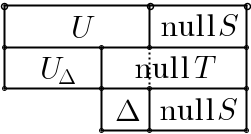
\includegraphics[width=88pt]{diagram3B-2}$}\hText{$
	\Blind{$\range S\xlongleftarrow{S}{}$}$U_{\Delta}\xlongrightarrow{T}\range T\\[-7pt]$
	$\range S\xlongleftarrow{S}\oplus\\[-6pt]$
	\Blind{$\range S\xlongleftarrow{S}{}$}$\Delta\xlongrightarrow{T}\zeroSubs}\MathLeftMid{l}{$
	Becs $\Delta=\null T\mmid_U=\null T\cap\Range\BigPar{S\mmid_U}{^{-1}}.\\$
	Thus \,$E=T\BigPar{S\mmid_{U}}{^{-1}}$ is not inje $\Longleftrightarrow\Delta\neq\zeroSubs.\\$
	In other words, $\range S\mmid_\Delta=\null E,\\$
	while $E\mmid_{\cdots}:\range S\mmid_{U_\Delta}\rightarrow\range T$ is iso.$}$\par\vspace{6pt}\quad
\AComm Let $E_1\in\Lm{U_{\Delta}\oplus\null T,U_{\Delta}},$ and $E_2$ be an iso of $\range S\mmid_{U_{\Delta}}$ onto $\range T.$\parCom\quad
Define $E_1\mmid_{U_{\Delta}}=I\mmid_{U_{\Delta}},$ and $E_2=T\BigPar{S\mmid_{U_{\Delta}}}{^{-1}}.$ \;Then $T=E_2SE_1.$\par\vspace{4pt}\quad
\ACoro If $\null S=\null T.$ Then $\Delta=\zeroSubs,U_{\Delta}=U.$ \Sbra[3pt]{{\tgsl Req $W$ Finide}} \;By (3.D.3),\parCor\quad
we can extend inje $T\BigPar{S\mmid_{U}}{^{-1}}\in\Lm[\BigPar]{\range S,W}$ to inv $E\in\Lm{M,W}.$\vspace{6pt}\par\quad
\Or \Sbra[3pt]{{\tgsl Req $\range S$ Finide}} \;Let $B_{\range S}=\Par{Sv_1,\dots,Sv_n}$. Then \uline{$V=\Span{v_1,\dots,v_n}\oplus\null S$.}\par\quad
Define $E\in\Lm{\range S,W}$ by $E\Par{Sv_i}=Tv_i.$ \;Extend to $E\in\Lm{M,W}.$\par\quad
Hence $\forall v=\sum_{i=1}^na_iv_i+u\in V,\,\,$\uline{$\BigPar{\exists\,!\,u\in\null S\subseteq\null T\,},\,Tv=\sum_{i=1}^na_iTv_i+0$}${}=E\BigBigPar{{\sum_{i=1}^na_iSv_i+0}}.$\PfEnd\Anchor{3D4}\vspace{6pt}\quad
\ACoro \Sbra[3pt]{{\tgsl Req $W$ Finide}} \;Supp $\null S=\null T.$ We show $\exists$ inv $E\in\Lm{M,W},T=ES.$\par\quad
Redefine $E\in\Lm{M,W}$ by $E\Par{Tv_i}=Sv_i,\;E\Par{w_j}=x_j,$ for each $Tv_i$ and $w_j.$ Where:\par\quad
Let $B_{\range T}=\Par{Tv_1,\dots,Tv_m},B_W=\Par{Tv_1,\dots,Tv_m,w_1,\dots,w_n},B_U=\Par{v_1,\dots,v_m}.$\par\quad
Now $V=U\oplus\null T=U\oplus\null S\Rightarrow B_{\range S}=\BigPar{Sv_1,\dots,Sv_m}.$ Let $B_M=\Par{Sv_1,\dots,Sv_m,x_1,\dots,x_n}.$\PfEnd 
\SepLine

\ProblemN{\Anchor{3B25}{25}}{
	\TextA{Supp {\FontNorm$S\in\Lm{Y,W},T\in\Lm{V,W},$} and $\range T\subseteq\range S.$ Prove $\exists\,E\in\Lm{V,Y},T = SE$.}
}Let $Y=U\oplus\null S$\vspace{-4pt}\parSol{}
$\Rightarrow S\mmid_U:U\rightarrow\range S$ is iso. Becs $\Par{S\mmid_U}{^{-1}}:\overset{\range T\:\subseteq}{{\range S}}\rightarrow U.$\par\quad
\uline{Define $E=\BigPar{S\mmid_U}{^{-1}}T=\BigPar{S\mmid_U}{^{-1}}\Big|{_{\range T}}T\in\Lm{V,U}\subseteq\Lm{V,Y}.$}\PfEnd\vspace{-20pt}\quad
\!\!\!$\hText{\\[6pt]$
	\AComm Let $U_1=U.$ Let $U_2\oplus\null T=V.\\$
	Let $U_{1\Delta}=\Range\BigPar{S\mmid_{U_1}}{^{-1}}\Big|{_{\range T}}\subseteq U_1=\Delta\oplus U_{1\Delta}.\\$
	\Or Let $U_{1\Delta}=\range E\mmid_{U_2}.$ \,Let $\Delta\oplus\range E\mmid_{U_2}=U_1.$
%	Thus $U_1\oplus\null S=U_{1\Delta}\oplus{}$\uline{$\Par{\Delta\oplus\null S}$}${}=U_2\oplus{}$\uline{$\null T$}$.\\[-10pt]$
%	\Blind{Thus $U_1\oplus\null S=U_{1\Delta}\oplus{}$}$\qquad\text{\tiny|}\qquad\qquad\qquad\qquad\text{\tiny|}\\[-20pt]$
%	$\hspace{164.2pt}\underset{\text{iso, \;if finide.}}{\uline{\;\qquad\qquad\qquad\qquad\hspace{-2pt}}}$
$}\qquad\qquad\qquad\quad$\FontSmall$\hText{U_1\xlongrightarrow[S]{inv}\range S\\[-8pt]\;\text{\small|\:|}\qquad\qquad\text{\small|\:|}\\[-6pt]\;\Delta\,\xlongrightarrow[S]{inv}\range S\mmid_{\Delta}\\[-8pt]\;\oplus\qquad\quad\;\;\oplus\\[-6pt]\,U_{1\Delta}\xlongrightarrow[S]{inv}\range T\xlongleftarrow[T]{inv}U_2\\[-8pt]\,\;\uparrow\qquad\qquad\qquad\qquad\quad|\\[-19pt]\,\;\,\underset{inv\;\;E\def\envFontA{\normalsize}\mmid_{U_2}}{{\uline{\qquad\qquad\qquad\qquad\qquad\!\!}}}}$\FontNorm\par\vspace{2pt}\quad
%\ACoro If $\Delta=\zeroSubs,$ then $U_1=U_{1\Delta}\Rightarrow\range S=\range T.$ 又 $\null S,\null T$ are iso.\par\quad
%By (3.D.3), we can re-extend inje $E\mmid_{U_2}\in\Lm[\BigPar]{U_2,U_1\oplus\null S}$ to inv $E\in\Lm[\BigPar]{U_2\oplus\null T,U_1\oplus\null S}.$\par\vspace{4pt}\quad
%Thus we have $\Delta\neq\zeroSubs\Longleftrightarrow E\mmid_{U_2}\in\Lm{U_2,V}$ cannot be re-extended to inv $E\in\Lm{V}$ freely.
\Sbra[3pt]{{\tgsl Req $\range T$ Finide}} \;Let $B_{\range T}=\Par{Tv_1,\dots,Tv_n}.$ Now $B_{U_2}=\Par{v_1,\dots,v_n}.$\par\quad
\uline{Let $S\Par{u_i}=Tv_i$ for each $Tv_i.$} \;Define $E$ with each $Ev_i=u_i,Ex=0$ for $x\in\null T.$\PfEnd\vspace{4pt}\quad
\AComm \Sbra[3pt]{{\tgsl Req $V$ Finide}} \;Note that $\dim U_2\leqslant\dim U_1\Longrightarrow\dim\null T=p\geqslant q=\dim\null S.$\parCom\quad
Let $B_{\null T}=\Par{x_1,\dots,x_p},B_{\null S}=\Par{y_1,\dots,y_q}.$ Redefine $E:v_i\mapsto u_i,\;x_k\mapsto y_k,\;x_j\mapsto 0,$\parCom\quad
for each $i\in\Bra{1,\dots,\dim U_2},k\in\Bra{1,\dots,\dim\null S}=K,j\in\Bra{1,\dots,\dim\null T}\Backslash[\Big]K.$\parCom\quad
Note that $\Par{u_1,\dots,u_n}$ is liney indep. Let $X=\Span{x_1,\dots,x_q}\oplus\Span{v_1,\dots,v_n}.$\parCom\quad
Now $E\mmid_X$ is inje, but cannot be re-extend to inv $E\in\Lm{V,Y}$ suth $T=SE.$\par\Anchor{3D5}\vspace{4pt}\quad
\ACoro \Sbra[3pt]{{\tgsl Req $V$ Finide}} \;If $\range T=\range S,$ then $\dim\null T=\dim\null S=p.$\parCor\quad
Redefine $E$ by $Ev_i=u_i,\;Ex_j=y_j$ for each $v_i$ and $x_j.$ Then $E\in\Lm{V,Y}$ is inv.\PfEnd
\SepLine

\Anchor{3BC2425}\BulletPointX\AComm Supp $S,T\in\Lm{V,W}.$ Then $\range S=\range T\notRightarrow\null S,\null T$ iso.\TextB{}
\AExa Forwd shift optor on $\Fbb^{\infty}$ and backwd shift optor on $\Bra{\Par{0,x_1,x_2,\cdots}\in\Fbb^{\infty}}.$\TextB{\vspace{2pt}}
While $\null S=\null T\Longleftrightarrow E:Sv\mapsto Tv$ and $E^{-1}:Tv\mapsto Sv$ well-defined $\Rightarrow \range S,\range T$ iso.
\SepLine

\ProblemB[]{
	\TextB{Supp $S,T\in\Lm{V,W}.$}
}
\Anchor{3D6}\ProblemBnoor{{3.D.6}}{
	\TextA{Supp $V$ and $W$ are finide. $\dim\null S=\dim\null T=n.$}
	\TextA{Prove $S=E_2 T E_1,\exists$ inv $ E_1\in\Lm{V}, E_2\in\Lm{W}.$}
}$\text{Define}\;\,E_1:\,\,\,\,\, v_i\mapsto r_i\,\,;\quad u_j\mapsto s_j;$\quad for each $i\in\Bra{1,\dots,m},j\in\Bra{1,\dots,n}.$\parSol{}
$\text{Define}\;\,E_2:Tv_i\mapsto Sr_i\,\,;\;\;x_j\mapsto y_j;$\quad for each $i\in\Bra{1,\dots,m},j\in\Bra{1,\dots,n}.$
Where:\parSol{\vspace{2pt}}
$\MathLeftrightMid{l}{$
	Let $B_{\range T}=\Par{Tv_1,\dots,Tv_m};\;B_{\range S}=\Par{Sr_1,\dots,Sr_m}.\\ $
	Let $B_W=\Par{Tv_1,\dots,Tv_m,x_1,\dots,x_p};\;B_W'=\Par{Sr_1,\dots,Sr_m,y_1,\dots,y_p}.\\ $
	Let $B_{\null T}=\Par{u_1,\dots,u_n};\;B_{\null S}=\Par{s_1,\dots,s_n}.\\ $
	Thus $B_V=\Par{v_1,\dots,v_m,u_1,\dots,u_n};\;B_V'=\Par{r_1,\dots,r_m,s_1,\dots,s_n}.}\hMath{c}{}{}{\therefore\;E_1,E_2$ are inv$ \\ $and $S=E_2 TE_1.}$\PfEnd
\SepLine[0pt][\Blind{\BulletPointX} ]

\ProblemB{
	(a) \TextB{Supp $T=ES$ and $E\in\Lm{W}$ is inv. Prove $\null S=\null T.$\vspace{2pt}}
	(b) \TextB{Supp $T=SE$ and $E\in\Lm{V}$ is inv. Prove $\range S=\range T.$\vspace{2pt}}
	(c) \TextB{Supp $T=E_2SE_1$ and $E_1\in\Lm{V},E_2\in\Lm{W}$ are inv.}
	\Hc\TextB{Prove $\dim\null S=\dim\null T.$}
}(a) $v\in\null T\Longleftrightarrow Tv=0=E\Par{Sv}\Longleftrightarrow Sv=0\Longleftrightarrow v\in\null S.$\parSol{}
(b) $w\in\range T\Longleftrightarrow\exists\,v\in V,w=Tv=S\Par{Ev}\Longleftrightarrow w\in\range S.$\parSol{}
(c) By the {\COROLLARY} in Exe (22), $\dim\null E_2SE_1\xlongequal[\text{inv}]{E_2}\dim\null SE_1\xlongequal[\text{inv}]{E_1}\dim\null S=\dim\null T.$\PfEnd
\SepLine

\ProblemN{\Anchor{3B28}28}{
	\TextA{Supp $T\in\Lm{V,W}.$ Let $\Par{Tv_1,\dots,Tv_m}$ be a bss of $\range T$ and each $w_i=Tv_i.$}
	\PrePa\TextA{Prove $\exists\,\varphi_1,\dots,\varphi_m\in\Lm{V,\Fbb}$ suth $\forall v\in V,Tv=\varphi_1\Par{v}w_1+\dots+\varphi_m\Par{v}w_m$.\vspace{2pt}}
	\PrePb{\FontSmall\Sbra{4E 3.F.5}} \TextA{$\forall v\in V,\exists\,!\,\varphi_i\Par{v}\in\Fbb,Tv=\varphi_1\Par{v}w_1+\dots+\varphi_m\Par{v}w_m.$\vspace{1pt}}\Anchor{3F4e5}
	\Blind{\PrePb{\FontSmall\Sbra{4E 3.F.5}}} \TextA{Thus defining each $\varphi_i:V\rightarrow\Fbb.$ \;Show each $\varphi_i\in\Lm{V,\Fbb}.$}
}{\FontSmall\tgsl The answer for (b) with (b) itself is the answer for (a).}\par\quad
(b) $\sum_{i=1}^m\varphi_i\Par{u+\lambda v}w_i=T\Par{u+\lambda v}=Tu+\lambda Tv={\BigBigPar{{\sum_{i=1}^m\varphi_i\Par{u}w_i}}}+\lambda{\BigBigPar{{\sum_{i=1}^m\varphi_i\Par{v}w_i}}}.$\PfEnd\vspace{4pt}\quad\Hb
\Or $\forall v\in V,\exists\,!\,a_i\in\Fbb,Tv=a_1Tv_1+\dots+a_mTv_m.$ Let $B_{\SmallPar[1pt]{\range T}\apostrophe}=\Par{\psi_1, \dots, \psi_m}$.\par\quad\Hb
Then $\Sbra{T\apostrophe\Par{\psi_{i}}}\Par{v}=\BigPar{\psi_{i}\circ T}\Par{v}=a_i.$ \,Thus each $\varphi_i=\psi_i\circ T=T\apostrophe\Par{\psi_i}\in V\apostrophe.$\PfEnd\vspace{4pt}\quad
(a) $\Span{v_1,\dots,v_m}\oplus\null T=V\Rightarrow\forall v\in V,\exists\,!\,a_i\in\Fbb,u\in\null T,\;v=\sum_{i=1}^m a_i v_i+u.$\par\quad\Ha
Define $\varphi_i\in\Lm{V,\Fbb}$ by $\varphi_i\Par{v_j}=\delta_{i,j},\;\varphi_i\Par{u}=0$ for all $u\in\null T.$\par\quad\Ha
Linity: $\forall v,w\in V\,\Sbra{\exists\,!\,a_i,b_i\in\Fbb},\lambda\in\Fbb,\varphi_i\Par{v+\lambda w}=a_i+\lambda b_i=\varphi\Par{v}+\lambda\varphi\Par{w}.$\PfEnd
\SepLine

\ProblemN{\Anchor{3B29}{29}}{
	\TextA{Supp $\varphi\in\Lm{V,\Fbb}.$ Supp $\varphi\Par{u}\neq 0.$ Prove $V = \null\varphi\oplus\Bra{au :a\in\Fbb}.$\FontSmall\hfill By \TIPSN{4}, immed.}
}(a) $v=cu\in\null\varphi\cap\Span{u}\Rightarrow c\varphi\Par{u}=0\Rightarrow v=0.$ \;Now $\null\varphi\cap\Span{u}=\zeroSubs.$\parSol{}
(b) For $v\in V,$ let $a_v=\varphi\Par{v}.$ Then $v=\Sbra{v-\Par{a_v\big/a_u}u}+\Par{a_v\big/a_u}u\Rightarrow V=\null\varphi+\Span{u}.$\PfEnd\vspace{-3pt}
\SepLine

\ProblemN{\Anchor{3B30}{30}}{
	\TextA{Supp $\varphi,\beta\in\Lm{V,\Fbb}$ and $\null\varphi=\null\beta=\eta.$ Prove $\exists\,c\in\Fbb,\varphi=c\beta.$}
}If $\eta=V$, then $\varphi=\beta=0,$ done. Now by Exe (29),\parSol{}
$\varphi\Par{u}\neq 0\Longleftrightarrow V=\null\varphi\oplus\Span{u}\Longleftrightarrow V=\null\beta\oplus\Span{u}\Longleftrightarrow\beta\Par{u}\neq 0.$\parSol{}
\hspace{-5pt}$\hText{$
	Note that $\forall v\in V,\exists\,!\,u_0\in\eta,\;a_v\in\Fbb,v=u_0+a_vu\\$
	$\Rightarrow\varphi\Par{u_0+a_vu}=a_v\varphi\Par{u},\;\beta\Par{u_0+a_vu}=a_v\beta\Par{u}.}\;\MathLeftMid{l}{$Let $c={}${\Large\envFontSmall$\frac{\varphi\Par{u}}{\beta\Par{u}}$}${}\in\nonzeroFbb.}$\PfEnd%\vspace{6pt}
%\AComm Convly, if $\varphi=c\beta,\exists\,c\in\nonzeroFbb.$ \,Then $\null\beta=\Null\Par{c\varphi}=\null\varphi.$\parCom
%Note that $c\varphi=E\circ\varphi,$ where $E\in\Lm{\Fbb}:x\rightarrow cx,$ and $E$ is inv.
\SepLine

\Anchor{3F4e6}\ProblemBnoor{{4E 3.F.6}}{
	\TextB{Supp $\varphi,\beta\in\Lm{V,\Fbb}.$ Prove $\null \beta\subseteq\null\varphi\Longleftrightarrow\varphi=c\beta,\exists\,c\in\Fbb.$}
	\ACoro $\null \varphi=\null\beta\Longleftrightarrow\varphi=c\beta,\;\exists\,c\in\nonzeroFbb.$\TextB{}
}Using Exe (29) and (30).\par\quad
(a) If $\varphi=0,$ then done. Othws, supp $u\not\in\null\varphi\supseteq\null \beta.$\vspace{-4pt}\par\quad\Ha
Now $V=\null \varphi\oplus\Span{u}=\null \beta\oplus\Span{u}.$ By \Sbra{1.C \TIPSN{2}}, $\null \varphi=\null \beta.$ \;Let $c={}${\Large\envFontSmall$\frac{\varphi\Par{u}}{\beta\Par{u}}$}.\vspace{2pt}\par\quad\Ha
\Or We discuss in two cases. If $\null \beta=\null \varphi$, or if $\varphi=0,$ then done. Othws,\par\quad\Ha
$\exists\,u\apostrophe\in\null \varphi\Backslash[\Big]\null \beta,\,\exists\,u\not\in\null\varphi\supsetneq\null\beta\Rightarrow V=\null \beta\oplus\Span{u\apostrophe}=\null \beta\oplus\Span{u}.$\par\quad\Ha
\hspace{-5pt}$\hText{$
	$\forall v \in V, v=w+au=w\apostrophe+bu\apostrophe,\,\exists\,!\,w, w\apostrophe\in\null \beta\\$
	Thus $\varphi\Par{w+au}=a\varphi\Par{u},\,\,\beta\Par{w\apostrophe+bu}=b\beta\Par{u\apostrophe}.}\;\MathLeftMid{l}{$ Let $c={}${\Large\envFontSmall$\frac{a\varphi\Par{u}}{b\beta\Par{u\apostrophe}}$}${}\in\nonzeroFbb.$ \;Done.$}$\vspace{6pt}\par\quad\Ha
\NOTICE that by (b) below, we have $\null \varphi\subseteq\null \beta,$ ctradic the asum.\vspace{6pt}\par\quad
(b) If $c=0$, then $\null \varphi=V\supseteq\null \beta$, done. Othws, becs $v\in\null \beta\Longleftrightarrow v\in\null \varphi.$\PfEnd\vspace{4pt}\quad
\Or By Exe (24), $\null \beta\subseteq\null \varphi\Longleftrightarrow\exists\,E\in\Lm{\Fbb},\varphi=E\circ\beta.$ \Sbra{ If $E$ is inv. Then $\null \beta=\null \varphi.$ }\par\quad
Now $\exists\,E\in\Lm{\Fbb},\varphi=E\circ\beta\Longleftrightarrow\exists\,c=E\Par{1}\in\Fbb,\varphi=c\beta.$ \Sbra{ $E$ is inv $\Longleftrightarrow E\Par{1}\neq 0\Longleftrightarrow c\neq 0.$ }\PfEnd
\SepLine

\ChEnd

\vfill\ChDecl{Ch3C}{3$\cdot$C}{}

\vspace{8pt}

\Anchor{3CN3.3032}\BulletPointX\NoteFor{[3.30, 32]}\;\;{\tgsl matrix of span}\TextB{}
Supp $L_{\alpha}=\Par{\alpha_1,\dots,\alpha_n}$ and $L_{\beta}=\Par{\beta_1,\dots,\beta_m}$ are in a vecsp $V.$\TextB{}
Let each $\alpha_k=A_{1,k}\beta_1+\dots+A_{m,k}\beta_m,$ forming $A=\Mt{\spn L_\beta\supseteq L_{\alpha}}\in\Fbb^{m,n}.$\TextB{\vspace{3pt}}
Which is {\tgsl the matrix of span}. \;Then ${\normalsize\begin{pmatrix}\beta_1 &\hspace{-6pt} \cdots &\hspace{-6pt} \beta_m\end{pmatrix}\begin{pmatrix}
	A_{1,1} &\hspace{-6pt} \cdots &\hspace{-6pt} A_{1,n}\\[-4pt]
	\vdots	&\hspace{-6pt} \ddots &\hspace{-6pt} \vdots \\[-4pt]
	A_{m,1} &\hspace{-6pt} \cdots &\hspace{-6pt} A_{m,n}
\end{pmatrix}}={\normalsize\begin{pmatrix}\alpha_1 &\hspace{-6pt} \cdots &\hspace{-6pt} \alpha_n\end{pmatrix}}.$\TextB{\vspace{6pt}}
(a) Supp $m=n.$ If $\Par{A_{\cdot,1},\dots,A_{\cdot,n}}$ is a bss of $\Fbb^{n,1}.$ We show $L_{\alpha}$ liney indep $\Longleftrightarrow L_{\beta}$ liney indep.\TextB{}
\Ha ($\Leftarrow$) Immed. ($\Rightarrow$) Asum $L_{\beta}$ is liney dep and $\beta_j=c_1\beta_1+\dots+c_{j-1}\beta_{j-1}.$ By ctradic.\PfEnd\vspace{2pt}\TextB{}
(b) Supp $m\geqslant n.$ If $L_{\beta}$ liney indep. We show $\Par{A_{\cdot,1},\dots,A_{\cdot,n}}$ liney indep $\Longleftrightarrow L_{\alpha}$ liney indep.\TextB{}
\Hb ($\Rightarrow$) Immed. ($\Leftarrow$) By ctradic.\PfEnd\TextB{}
\Hb\AComm $\Mt{\spn L_{\beta}\supseteq L_\alpha}=\Mt{I,L_{\alpha},L_{\beta}}\Longleftrightarrow L_{\alpha},L_{\beta}$ liney indep $\Rightarrow\Par{A_{\cdot,1},\dots,A_{\cdot,n}}$ liney indep.\parCom{\Hb\IndentB}
Where $I$ is the id optor retr to $\spn L_{\alpha}\subseteq\spn L_{\beta}.$
\vspace{3pt}\TextB{}
(c) Supp $m<n.$ Then $\Par{A_{\cdot,1},\dots,A_{\cdot,n}}$ is liney dep, so is $L_{\alpha}.$\TextB{\vspace{5pt}}
Supp $T\in\Lm{V,W}$ and $B_V=\Par{v_1,\dots,v_m},B_W=\Par{w_1,\dots,w_n}.$\TextB{}
Then $\Mt{T,B_V\hspace{1pt},B_W}=\Mt[\BigPar]{\spn B_W\supseteq\Par{Tv_1,\dots,Tv_m}}.$ \; \AComm See also (4E 3.D.23).
\SepLine

\pagebreak
\def\fT{\mT}\def\fC{\mC}\def\fR{\mR}\def\fP{\mE}

\Anchor{3CNTrspose}\Anchor{3F33}\BulletPointX\NoteFor{Trspose}\;\;{\FontSmall\Sbra{3.F.33}}\;Define $\fT:A\rightarrow A^t.$ By [3.111], $\fT$ is liney. Becs $\Par{A^t}{^t}=A.$ \TextB{}
$\fT^2=I,\,\fT=\fT^{-1}\Rightarrow \fT$ is iso of $\Fbb^{m,n}$ onto $\Fbb^{n,m}.$ \;Define $\fC_k:A\rightarrow A_{\cdot,k},\;\fR_j:A\rightarrow A_{j,\cdot},\;\fP_{j,k}:A\rightarrow A_{j,k}.$\TextB{}
%Let $A={}{\small\begin{pmatrix}1 &\hspace{-6pt} 2 &\hspace{-6pt} 3\\[-4pt] 4 &\hspace{-6pt} 5 &\hspace{-6pt} 6\end{pmatrix}}\Rightarrow A^t={}{\small\begin{pmatrix}1 &\hspace{-6pt} 4\\[-4pt] 2 &\hspace{-6pt} 5\\[-4pt] 3&\hspace{-6pt} 6\end{pmatrix}}.$ \;$\MathLeftMid{l}{$
%	\!\!$\Par{A_{2,\cdot}}{^t}={}{\small\begin{pmatrix}4 &\hspace{-6pt} 5 &\hspace{-6pt} 6\end{pmatrix}}{^t}\neq{}{\small\begin{pmatrix}2 &\hspace{-6pt} 5\end{pmatrix}}{}=\Par{A^t}{_{2,\cdot}}$ \;Simlr for all $A_{j,\cdot},A_{\cdot,k},$ and $A_{j,k}.\\[2pt]$
%	\!\!Thus in general, $\fC_k\fT\neq \fT\fC_k,\;\fR_j\fT\neq \fT\fR_j,$ \,and $\fP_{j,k}\fT\neq \fT\fP_{j,k},}$\TextB{\vspace{6pt}}
%But $\Par{A_{2,\cdot}}{^t}=\Par{A^t}{_{\cdot,2}}.$ \;
Now we show (a) \uline{$\fT\fR_j=\fC_j\fT,$} \,(b) \uline{$\fT\fC_k=\fR_k\fT,$} \,and (c) \uline{$\fT\fP_{j,k}=\fP_{k,j}\fT.$}\TextB{\vspace{2pt}}
So that $\fT\fC_k\fT=\fR_k,\;\fT\fR_j\fT=\fC_j,$ \,and $\fT\fP_{j,k}\fT=\fP_{k,j}.$\TextB{\vspace{4pt}}
Let $A={}{\normalsize\begin{pmatrix}A_{1,1} &\hspace{-6pt} \cdots &\hspace{-6pt} A_{1,n}\\[-4pt] \vdots &\hspace{-6pt} \ddots &\hspace{-6pt} \vdots\\[-4pt] A_{m,1} &\hspace{-6pt} \cdots &\hspace{-6pt} A_{m,n}\end{pmatrix}}\Rightarrow A^t={}{\normalsize\begin{pmatrix}A_{1,1} &\hspace{-6pt} \cdots &\hspace{-6pt} A_{m,1}\\[-4pt] \vdots &\hspace{-6pt} \ddots &\hspace{-6pt} \vdots\\[-4pt] A_{1,n} &\hspace{-6pt} \cdots &\hspace{-6pt} A_{m,n}\end{pmatrix}}.$ \;$\MathLeftMid{l}{\!\!$
Note that $\Par{A_{j,k}}{^t}=A_{j,k}=\Par{A^t}_{k,j}.$ Thus (c) holds.$\\$
\!\!And $\Par{A_{\cdot,k}}{^t}={}{\small\begin{pmatrix}A_{1,k} &\hspace{-6pt} \cdots &\hspace{-6pt}A_{m,k}\end{pmatrix}}{}={}{\small\begin{pmatrix}A^t_{k,1} &\hspace{-6pt} \cdots &\hspace{-6pt}A^t_{k,m}\end{pmatrix}}{}=\Par{A^t}{_{k,\cdot}}\\$
\!\!$\Longrightarrow$ (b) holds. Simlr for (a).$}$\par\vspace{8pt}
\SepLine

\Anchor{3CN3.48}\BulletPointX\NoteForSmall{[3.48]}\vspace{-12pt}\par\quad
\!\!{\normalsize$\underbrace{\begin{pmatrix}
  1 &\hspace{-4pt} 2 \\[-2pt]
  3 &\hspace{-4pt} 4
\end{pmatrix}}_{A}\underbrace{\begin{pmatrix}
  5 &\hspace{-4pt} 6 &\hspace{-4pt} 7 \\[-2pt]
  8 &\hspace{-4pt} 9 &\hspace{-4pt} 10
\end{pmatrix}}_{B}{}={}\begin{pmatrix}
  \begin{pmatrix} 1 &\hspace{-4pt} 2\end{pmatrix}
  \begin{pmatrix} 5 \\[-2pt] 8\end{pmatrix}
  &\hspace{-4pt}
  \begin{pmatrix} 1 &\hspace{-4pt} 2\end{pmatrix}
  \begin{pmatrix} 6 \\[-2pt] 9\end{pmatrix}
  &\hspace{-4pt}
  \begin{pmatrix} 1 &\hspace{-4pt} 2\end{pmatrix}
  \begin{pmatrix} 7 \\[-2pt] 10\end{pmatrix}
  \\[0pt]
  \begin{pmatrix} 3 &\hspace{-4pt} 4\end{pmatrix}
  \begin{pmatrix} 5 \\[-2pt] 8\end{pmatrix}
  &\hspace{-4pt}
  \begin{pmatrix} 3 &\hspace{-4pt} 4\end{pmatrix}
  \begin{pmatrix} 6 \\[-2pt] 9\end{pmatrix}
  &\hspace{-4pt}
  \begin{pmatrix} 3 &\hspace{-4pt} 4\end{pmatrix}
  \begin{pmatrix} 7 \\[-2pt] 10\end{pmatrix}
\end{pmatrix}{}={}\begin{pmatrix} 21 &\hspace{-4pt} 24 &\hspace{-4pt} 27 \\[-2pt] 47 &\hspace{-4pt} 54 &\hspace{-4pt} 61\end{pmatrix}$}\vspace{8pt}\par
\SepLine

\Anchor{3CN3.47}\BulletPointX\NoteForSmall{[3.47]}\,\, $\BigPar{AC}{_{j,k}}=\sum_{r=1}^n A_{j,r}C_{r,k}=\sum_{r=1}^n \BigPar{A_{j,\cdot}}_{1,r}\BigPar{C_{\cdot,k}}_{r,1}=\BigPar{A_{j,\cdot}C_{\cdot,k}}_{1,1}=A_{j,\cdot}C_{\cdot,k}$\PfEnd\vspace{6pt}
\Anchor{3CN3.49}\BulletPointX\NoteForSmall{[3.49]} ${\BigSbra{\BigPar{AC}_{\cdot,k}}}_{j,1}=\BigPar{AC}_{j,k}=\sum_{r=1}^n A_{j,r}C_{r,k}=\sum_{r=1}^n A_{j,r}\BigPar{C_{\cdot,k}}_{r,1}=\BigPar{AC_{\cdot,k}}_{j,1}$\PfEnd\vspace{6pt}\Anchor{3C10}
\BulletPointX\Exercise{10}\qquad\hspace{5pt}${\BigSbra{\BigPar{AC}_{j,\cdot}}}_{1,k}=\BigPar{AC}_{j,k}=\sum_{r=1}^n A_{j,r}C_{r,k}=\sum_{r=1}^n \BigPar{A_{j,\cdot}}_{1,r}C_{r,k}=\BigPar{A_{j,\cdot}C}_{1,k}$\PfEnd\vspace{6pt}
\BulletPointX\AComm For [3.49], let $B_U=\Par{u_1,\dots,u_p},B_V=\Par{v_1,\dots,v_n},B_W=\Par{w_1,\dots,w_m}.$\vspace{2pt}\parCom{}\IndentB{}
And $C=\Mt{T,B_U,B_V}\in\Fbb^{n,p},A=\Mt{S,B_V,B_W}\in\Fbb^{m,n}.$\vspace{1pt}\parCom{}\IndentB{}
Then $\Mt{Tu_k,B_V}=C_{\cdot,k}\Rightarrow\Mt[\BigPar]{S\Par{Tu_k},B_W}=AC_{\cdot,k}\,,$ \;又 $\Mt[\BigBigPar]{\Par{ST}\Par{u_k},B_W}=\Par{AC}{_{\cdot,k}}$\PfEnd\vspace{4pt}\parCom{}\IndentB{}
By {\NOTEFOR} Transpose, $\BigPar{AC}{_{j,\cdot}}=\BigSbra{\BigBigPar{\BigPar{AC}{^t}}{_{\cdot,j}}}{^t}=\BigPar{C^t\Par{A^t}{_{\cdot,j}}}{^t}=\BigPar{\Par{A^t}{_{\cdot,j}}}{^t}C=A_{j,\cdot}C$\PfEnd
\SepLine

\Anchor{3C9}\BulletPointX\NoteForSmall{[3.52]}\;\;$A\in\Fbb^{m,n},c\in\Fbb^{n,1}\Rightarrow Ac\in\Fbb^{m,1}.$\hfill By \Sbra{4E 3.51(a)}, $\BigPar{Ac}{_{\cdot,1}}=c_1A_{\cdot,1}+\dots+c_nA_{\cdot,n}.$\;\;\!\,\PfEnd\vspace{4pt}\quad
\Or $\because\;\BigPar{Ac}{_{j,1}}=\sum_{r=1}^n A_{j,r}c_{r,1}=\BigSbra{\sum_{r=1}^n\BigPar{A_{\cdot,r}c_{r,1}}}_{j,1}=\BigPar{c_1 A_{\cdot,1}+\dots+c_n A_{\cdot,n}}_{j,1}$\vspace{1pt}\par\quad
\Blind{\Or}$\therefore\;\,Ac=A_{\cdot,\cdot}c_{\cdot,1}=\sum_{r=1}^n A_{\cdot,r}c_{r,1}=c_1 A_{\cdot,1}+\dots+c_n A_{\cdot,n}$\;\;\Or $\BigPar{Ac}{_{j,1}}=\BigPar{Ac}{_{j,\cdot}}=A_{j,\cdot}c\in\Fbb.$\PfEnd\vspace{2pt}\quad
%$={}{\small\begin{pmatrix}A_{j,1}&\hspace{-6pt}\cdots&\hspace{-6pt}A_{j,n}\end{pmatrix}\begin{pmatrix}c_1\\[-4pt]\vdots\\[-6pt]c_n\end{pmatrix}}.$\PfEnd\vspace{-2pt}\quad
\Or Let $B_V=\Par{v_1,\dots,v_n}.$ Now $Ac=\Mt{Tv,B_W}=\Mt[\BigPar]{T\Par{c_1v_1+\dots+c_nv_n}}=c_1A_{\cdot,1}+\dots+c_nA_{\cdot,n}.$\PfEnd
%$c_1{\small\begin{pmatrix}A_{1,1}\\[-4pt]\vdots\\[-4pt]A_{m,1}\end{pmatrix}}+\dots+c_n{\small\begin{pmatrix}A_{1,n}\\[-4pt]\vdots\\[-4pt]A_{m,n}\end{pmatrix}}.$\PfEnd
\SepLine

\Anchor{3C11}\BulletPointX\Exercise{11}\;\;$a\in\Fbb^{1,n},C\in\Fbb^{n,p}\Rightarrow aC\in\Fbb^{1,p}.$\hfill By \Sbra{4E 3.51(b)}, $\BigPar{aC}{_{1,\cdot}}=a_1C_{1,\cdot}+\dots+a_nC_{n,\cdot}.$\;\;\!\,\PfEnd\vspace{4pt}\quad
\Or $\because\;\BigPar{aC}{_{1,k}}=\sum_{r=1}^n a_{1,r}C_{r,k}=\BigSbra{\sum_{r=1}^n a_{1,r}\BigPar{C_{r,\cdot}}}_{1,k}=\BigPar{a_1 C_{1,\cdot}+\dots+a_n C_{n,\cdot}}_{1,k}$\vspace{2pt}\par\quad
\Blind{\Or}$\therefore\;\,aC=a_{1,\cdot}C_{\cdot,\cdot}=\sum_{r=1}^n a_{1,r}C_{r,\cdot}=a_1 C_{1,\cdot}+\dots+a_n C_{n,\cdot}$\;\;\Or $\BigPar{aC}{_{1,k}}=\BigPar{aC}{_{\cdot,k}}=aC_{\cdot,k}\in\Fbb.$\PfEnd\vspace{4pt}\quad
%$={\small\begin{pmatrix}a_1&\hspace{-6pt}\cdots&\hspace{-6pt}a_n\end{pmatrix}\begin{pmatrix}C_{1,k}\\[-4pt]\vdots\\[-4pt]C_{n,k}\end{pmatrix}}.$\PfEnd\vspace{-2pt}\quad
\Or \;$aC=\BigBigPar{\Par{aC}{^t}}{^t}=\BigPar{C^ta^t}{^t}=\Sbra{a^t_1\Par{C^t}{_{\cdot,1}}+\dots+a^t_n\Par{C^t}{_{\cdot,n}}}{^t}=a_1C_{1,\cdot}+\dots+a_nC_{n,\cdot}.$\PfEnd
\SepLine

\Anchor{3CN4e3.51}\ProblemBnoor[]{4E 3.51}[\Sbra]{
	Supp $C\in\Fbb^{m,c},R\in\Fbb^{c,p}$. \hfill\Sbra{ See also {\NOTEFOR} [3.49] and Exe (10). }\TextB{\vspace{2pt}}
	(a) For $k=1,\dots,p,$\quad $\BigPar{CR}{_{\cdot,k}}=CR_{\cdot,k}=C_{\cdot,\cdot}R_{\cdot,k}=\sum_{r=1}^c C_{\cdot,r}R_{r,k}=R_{1,k}C_{\cdot,1}+\dots+R_{c,k}C_{\cdot,c}$\TextB{\vspace{3pt}}
	%\Ha\TextB{\large Which means that each cols $CR$ is a liney combina of the cols of $C.$\vspace{6pt}}
	(b) For $j=1,\dots,m,$\quad $\BigPar{CR}{_{j,\cdot}}=C_{j,\cdot}R=C_{j,\cdot}R_{\cdot,\cdot}=\sum_{r=1}^c C_{j,r}R_{r,\cdot}=C_{j,1}R_{1,\cdot}+\dots+C_{j,c}R_{c,\cdot}$\TextB{\vspace{2pt}}
	%\Hb\TextB{\large Which means that each rows $CR$ is a liney combina of the rows of $R.$}
}\BulletPointX\AExa $m=2,c=2,p=3.$\TextB{\vspace{2pt}}
%$\BigPar{AB}_{\cdot,1}=AB_{\cdot, 1}=\begin{pmatrix} 1 &\hspace{-4pt} 2\\[-2pt] 3 &\hspace{-4pt} 4\end{pmatrix}\begin{pmatrix} 5 \\[-2pt] 8\end{pmatrix}=5\begin{pmatrix}1\\[-2pt]3\end{pmatrix}+8\begin{pmatrix}2\\[-2pt]4\end{pmatrix}=\begin{pmatrix} 21\\[-2pt] 47\end{pmatrix}$;\TextB{}
$\BigPar{AB}{_{\cdot,2}}=AB_{\cdot, 2}=\begin{pmatrix} 1 &\hspace{-4pt} 2\\[-2pt] 3 &\hspace{-4pt} 4\end{pmatrix}\begin{pmatrix} 6 \\[-2pt] 9\end{pmatrix}=A_{\cdot,1}B_{1,2}+A_{\cdot,2}B_{2,2}=6\begin{pmatrix}1\\[-2pt]3\end{pmatrix}+9\begin{pmatrix}2\\[-2pt]4\end{pmatrix}=\begin{pmatrix} 24\\[-2pt] 54\end{pmatrix}$;\TextB{\vspace{2pt}}
%$\BigPar{AB}_{\cdot,3}=AB_{\cdot, 3}=\begin{pmatrix} 1 &\hspace{-4pt} 2\\[-2pt] 3 &\hspace{-4pt} 4\end{pmatrix}\begin{pmatrix} 7 \\[-2pt] 10\end{pmatrix}=7\begin{pmatrix}1\\[-2pt]3\end{pmatrix}+10\begin{pmatrix}2\\[-2pt]4\end{pmatrix}=\begin{pmatrix} 27\\[-2pt] 61\end{pmatrix}$;\TextB{}
$\BigPar{AB}{_{1,\cdot}}=A_{1,\cdot}B=\begin{pmatrix} 1 &\hspace{-4pt} 2\end{pmatrix}\begin{pmatrix} 5 &\hspace{-4pt} 6 &\hspace{-4pt} 7 \\[-2pt] 8 &\hspace{-4pt} 9 &\hspace{-4pt} 10\end{pmatrix}=A_{1,1}B_{1,\cdot}+A_{1,2}B_{2,\cdot}=1\begin{pmatrix} 5 &\hspace{-4pt} 6 &\hspace{-4pt} 7\end{pmatrix}+2\begin{pmatrix}8 &\hspace{-4pt} 9 &\hspace{-4pt} 10\end{pmatrix}=\begin{pmatrix} 21 &\hspace{-4pt} 24 &\hspace{-4pt} 27\end{pmatrix}$;\par\vspace{6pt}
%$\BigPar{AB}_{2,\cdot}=A_{2,\cdot}B=\begin{pmatrix} 3 &\hspace{-4pt} 4\end{pmatrix}\begin{pmatrix} 5 &\hspace{-4pt} 6 &\hspace{-4pt} 7 \\[-2pt] 8 &\hspace{-4pt} 9 &\hspace{-4pt} 10\end{pmatrix}=3\begin{pmatrix} 5 &\hspace{-4pt} 6 &\hspace{-4pt} 7\end{pmatrix}+4\begin{pmatrix}8 &\hspace{-4pt} 9 &\hspace{-4pt} 10\end{pmatrix}=\begin{pmatrix} 47 &\hspace{-4pt} 54 &\hspace{-4pt} 61\end{pmatrix}$;\par
\SepLine\pagebreak

\Anchor{3CNCRFact}\ProblemB{
	\hspace{0pt}\textsc{\Large CR Factoriz}\quad\vspace{3pt}Supp non0 $A\in\Fbb^{m,n}.$ \TextB{Prove, with $p$ below, that $\exists\,C\in\Fbb^{m,p},R\in\Fbb^{p,n},A=CR.$\vspace{3pt}}
	\PrePa\TextB{Supp $\col A=\Span[\BigPar]{A_{\cdot,1},\cdots,A_{\cdot,n}}\subseteq\Fbb^{m,1},\dim\col A=c,\text{ the col rank}.$ Let $p=c.$\vspace{3pt}}
	\PrePb\TextB{Supp $\row A=\Span[\BigPar]{A_{1,\cdot},\cdots,A_{m,\cdot}}\subseteq\Fbb^{1,n},\dim\row A=r,\text{ the row rank}.$ Let $p=r.$\vspace{3pt}}
}Using [4E 3.51]. Notice that $A\neq 0\Rightarrow c,r\geqslant 1.$\vspace{2pt}\par\quad
(a) Reduce to bss $B_C=\BigPar{C_{\cdot,1},\cdots,C_{\cdot,c}},$ forming $C\in\Fbb^{m,c}$. Then $\forall k\in\Bra{1,\dots,n},$\vspace{2pt}\par\quad\Ha
$A_{\cdot,k}=R_{1,k}C_{\cdot,1}+\dots+R_{c,k}C_{\cdot,c}=\BigPar{CR}{_{\cdot,k}}\;,\exists\,!\,R_{1,k},\cdots,R_{c,k}\in\Fbb,$ forming $R\in\Fbb^{c,n}.$ Thus $A=CR.$\vspace{4pt}\par\quad
(b) Reduce to bss $B_R=\BigPar{R_{1,\cdot},\cdots,R_{r,\cdot}},$ forming $R\in\Fbb^{r,n}$. Then $\forall j\in\Bra{1,\dots,m},$\vspace{2pt}\par\quad\Hb
$A_{j,\cdot}=C_{j,1}R_{1,\cdot}+\dots+C_{j,r}R_{r,\cdot}=\BigPar{CR}{_{j,\cdot}}\;,\exists\,!\,C_{j,1},\dots,C_{j,r}\in\Fbb,$ forming $C\in\Fbb^{m,r}.$ Thus $A=CR.$\PfEnd\vspace{6pt}
\AExa $A={}$ {\normalsize$\begin{pmatrix} 10 &\hspace{-4pt} 7 &\hspace{-4pt} 4 &\hspace{-4pt} 1 \\[-2pt] 26 &\hspace{-4pt} 19 &\hspace{-4pt} 12 &\hspace{-4pt} 5\\[-2pt] 46 &\hspace{-4pt} 33 &\hspace{-4pt} 20 &\hspace{-4pt} 7\end{pmatrix}$
	{$\xlongequal{\SmallPar{\text{I}}}$}
	$\begin{pmatrix} 1 &\hspace{-4pt} 0\\[-2pt] 0 &\hspace{-4pt} 1\\[-2pt] 2 &\hspace{-4pt} 1\end{pmatrix}\begin{pmatrix} 10 &\hspace{-4pt} 7 &\hspace{-4pt} 4 &\hspace{-4pt} 1\\[-2pt] 26 &\hspace{-4pt} 19 &\hspace{-4pt} 12 &\hspace{-4pt} 5\end{pmatrix}$
	{$\xlongequal{\SmallPar{\text{II}}}$}
	$\begin{pmatrix} 7 &\hspace{-4pt} 4\\[-2pt] 19 &\hspace{-4pt} 12\\[-2pt] 33 &\hspace{-4pt} 20\end{pmatrix}\begin{pmatrix} 2 &\hspace{-4pt} -1\\[-2pt] 1 &\hspace{-4pt} 0\\[-2pt] 0 &\hspace{-4pt} 1\\[-2pt] -1 &\hspace{-4pt} 2\end{pmatrix}$}\par\quad
(I) {\normalsize$\begin{pmatrix} 46 &\hspace{-4pt} 33 &\hspace{-4pt} 20 &\hspace{-4pt} 7 \end{pmatrix}=2\begin{pmatrix} 10 &\hspace{-4pt} 7 &\hspace{-4pt} 4 &\hspace{-4pt} 1\end{pmatrix}+\begin{pmatrix} 26 &\hspace{-4pt} 19 &\hspace{-4pt} 12 &\hspace{-4pt} 5\end{pmatrix}=\begin{pmatrix}2 &\hspace{-4pt} 1\end{pmatrix}\begin{pmatrix} 10 &\hspace{-4pt} 7 &\hspace{-4pt} 4 &\hspace{-4pt} 1\\[-2pt] 26 &\hspace{-4pt} 19 &\hspace{-4pt} 12 &\hspace{-4pt} 5\end{pmatrix}$}, using [4E 3.51(b)].\vspace{3pt}\par\quad\HI
{\small$\begin{pmatrix} 46 &\hspace{-4pt} 33 &\hspace{-4pt} 20 &\hspace{-4pt} 7 \end{pmatrix}$}${}\in\Span{A_{1,\cdot},A_{2,\cdot}},$ and $\Par{A_{1,\cdot},A_{2,\cdot}}$ is liney indep. Thus $B_R=\BigPar{A_{1,\cdot},A_{2,\cdot}}.$\par\vspace{6pt}\quad\EndI
(II) {\normalsize$\begin{pmatrix} 10\\[-2pt] 26\\[-2pt] 46\end{pmatrix}=2\begin{pmatrix} 7\\[-2pt] 19\\[-2pt] 33\end{pmatrix}-\begin{pmatrix} 4\\[-2pt] 12\\[-2pt] 20\end{pmatrix}; \quad \begin{pmatrix} 1\\[-2pt] 5\\[-2pt] 7\end{pmatrix}=-\begin{pmatrix} 7\\[-2pt] 19\\[-2pt] 33\end{pmatrix}+2\begin{pmatrix} 4\\[-2pt] 12\\[-2pt] 20\end{pmatrix}$}. \;Thus $B_C=\BigPar{A_{\cdot,2},A_{\cdot,3}}.$\vspace{6pt}\par
\SepLine

\Anchor{3CNCrankEqRrank}\BulletPointX\textsc{Col Rank = Row Rank}\quad Using CR Factoriz. Let $A=CY$ by (a) and $A=XR$ by (b).\TextB{}
(a) $A_{j,\cdot}=\BigPar{CY}{_{j,\cdot}}=C_{j,\cdot}Y=C_{j,1}Y_{1,\cdot}+\dots+C_{j,c}Y_{c,\cdot}\in\row A=\Span[\BigPar]{A_{1,\cdot},\cdots,A_{n,\cdot}}=\Span[\BigPar]{Y_{1,\cdot},\cdots,Y_{c,\cdot}}.$\TextB{}
(b) $A_{\cdot,k}=\BigPar{XR}{_{\cdot,k}}=XR_{\cdot,k}=R_{1,k}X_{\cdot,1}+\dots+R_{r,k}X_{\cdot,r}\in\col A=\Span[\BigPar]{A_{\cdot,1},\cdots,A_{\cdot,m}}=\Span[\BigPar]{X_{\cdot,1},\cdots,X_{\cdot,r}}.$\TextB{}
Thus (a) $\dim\row A=r\leqslant c=\dim\col A,$ and (b) $\dim\col A=c\leqslant r=\dim\row A.$\vspace{2pt}\PfEnd\TextB{}
\Or Apply the result of (a) to $A^t\in\Fbb^{n,m}\Rightarrow\dim\row A^t=\dim\col A=c\leqslant r=\dim\row A=\dim\col A^t.$\PfEnd
\SepLine

\Anchor{3C4e16}\ProblemBnoor{4E 16}{
	\TextB{Supp $A\in\Fbb^{m,n}\nonzero.$ Prove [P] $\rank A=1\Longleftrightarrow\exists\,c_j,d_k\in\Fbb,$ each $A_{j,k}=c_j\cdot d_k.$ [Q]\vspace{-2pt}}
}\par\quad
\!\Sbra[3pt]{{\tgsl Using CR Factoriz}}\par\quad
$P\Rightarrow Q:$ \;Immed.\par\vspace{-12pt}\quad
$Q\Rightarrow P:$ \;Becs $\;A={}${\normalsize$\begin{pmatrix}c_1 \\[-4pt] \vdots \\[-5pt] c_m \end{pmatrix}\begin{pmatrix}d_1 & \hspace{-6pt}\cdots & \hspace{-6pt}d_n\end{pmatrix}$}${}={}${\normalsize$\begin{pmatrix} c_1 d_1 & \hspace{-6pt}\cdots & \hspace{-6pt}c_1 d_n\\[-4pt] \vdots & \hspace{-6pt}\ddots & \hspace{-6pt}\vdots \\[-5pt] c_m d_1 & \hspace{-6pt}\cdots & \hspace{-6pt}c_m d_n \end{pmatrix}$} $\Longrightarrow\row A=\Spn${\FontSmall$\MathLeftrightBrace{l}{
	\!\begin{pmatrix}\uline{c_1} d_1 & \hspace{-6pt}\cdots & \hspace{-6pt}\uline{c_1} d_n\end{pmatrix},\\[-6pt] \;\;\;\qquad\vdots\\[-6pt]
	\!\begin{pmatrix}\uline{c_m} d_1 & \hspace{-6pt}\cdots & \hspace{-6pt}\uline{c_m} d_n\end{pmatrix}
}%=\Spn\MathLeftrightBrace{c}{\!\!\begin{pmatrix}d_1 & \hspace{-6pt}\cdots & \hspace{-6pt}d_n\end{pmatrix}\!\!\!}
$}.\par\vspace{0pt}\quad
\Blind{$Q\Rightarrow P:$ \;}\Or $\col A=\Spn${\normalsize$\MathLeftrightBrace{c}{\!\!\begin{pmatrix} c_1\uline{d_1} \\[-4pt] \vdots \\[-5pt] c_m\uline{d_1}\end{pmatrix},\dots,\begin{pmatrix} c_1\uline{d_n} \\[-4pt] \vdots \\[-5pt] c_m\uline{d_n}\end{pmatrix}\!\!\!}$}${}={}\Spn${\normalsize$\MathLeftrightBrace{c}{\!\!\begin{pmatrix}c_1 \\[-4pt] \vdots \\[-5pt] c_m\end{pmatrix}\!\!\!}$}.\PfEnd\vspace{12pt}\quad
%$\exists\,C={}${\normalsize$\begin{pmatrix}c_1 \\[-4pt] \vdots \\[-5pt] c_m \end{pmatrix}$}${}\in\Fbb^{m,1},R=\begin{pmatrix} d_1 & \hspace{-6pt}\cdots & \hspace{-6pt}d_n\end{pmatrix}\in\Fbb^{1,n}$ suth $A=CR.$
\!\Sbra[3pt]{{\tgsl Not Using CR Factoriz}}\vspace{-8pt}\par\quad
$Q\Rightarrow P:$\,\;Using [4E 3.51(a)]. Each $A_{\cdot,k}\in\Spn${\normalsize$\MathLeftrightBrace{c}{\!\!\begin{pmatrix}c_1 \\[-4pt] \vdots \\[-5pt] c_m\end{pmatrix}\!\!\!}$}. $\hText{$
	Then $\rank A=\dim\col A\leqslant 1\\$
	又 $A\neq 0\Rightarrow\dim\col A\geqslant 1.}$\vspace{-8pt}\par\quad
$P\Rightarrow Q:$\,\;Becs $\dim\col A=\dim\row A=1.$\vspace{4pt}\par\quad
\Blind{$P\Rightarrow Q:$\,\;}{\vspace{8pt}Let $c_j=\Frac{A_{j,1}}{A_{1,1}}=\Frac{A_{j,2}}{A_{1,2}}=\dots=\Frac{A_{j,n}}{A_{1,n}},\quad d_k'=\Frac{A_{1,k}}{A_{1,1}}=\Frac{A_{2,k}}{A_{2,1}}=\dots=\Frac{A_{m,k}}{A_{m,1}}.$}\par\quad
\Blind{$P\Rightarrow Q:$\,\;}{$\Rightarrow A_{j,k}=d_k' A_{j,1}=c_j A_{1,k}=c_j d_k' A_{1,1}=c_j d_k,$ where $d_k=d_k' A_{1,1}.$}\PfEnd
\SepLine\pagebreak

%Note that $T$ is inveritlbe $\Longleftrightarrow$ $T\apostrophe$ is inv. And $A^t=\Mt{T\apostrophe,B_{\beta}\apostrophe,B_{\alpha}\apostrophe}.$\par\quad
%(a) Supp $T$ is inv, so is $T\apostrophe$. Becs $\BigPar{T\apostrophe\Par{\varphi_1},\dots,T\apostrophe\Par{\varphi_m}}$ is liney indep.\par\quad\Ha
%\NOTICE that $T\apostrophe\Par{\varphi_i}=A^t_{1,i}\psi_1+\dots+A^t_{m,i}\psi_m.$ By the \Par{$\Delta$} part in (4E 3.C.17),\par\quad\Ha
%the cols of $A^t$, namely the rows of $A$, are liney indep.\par\quad
%(b) Supp the rows of $A$ are liney indep, so are the cols of $A^t$. \NOTICE that $A^t$ has $\dim V\apostrophe$ cols.
%Then $B_{\range T\apostrophe}=B_{V\apostrophe}=\BigPar{T\apostrophe\Par{\varphi_1},\dots,T\apostrophe\Par{\varphi_m}}.$ Thus $T\apostrophe$ is surj. Hence $T\apostrophe$ is inv, so is $T.$\par

\Anchor{3CT1}\ProblemBX{\TipsN{1}}{
	\TextA{Supp $T\in\Lm{V,W},\;B_V=\Par{v_1,\dots,v_n},B_W=\Par{w_1,\dots,w_m}.$\vspace{-1pt}}
	{\tgsl Let $L=\BigPar{Tv_{\alpha_1},\dots,Tv_{\alpha_k}},\;L_{\mM}=\BigPar{A_{\cdot,\alpha_1},\cdots,A_{\cdot,\alpha_k}},$ where each $\alpha_i\in\Bra{1,\dots,n}.$}\TextA{\vspace{1pt}}
	\PrePa\TextA{Show [P] $L$ is liney indep $\Longleftrightarrow L_{\mM}$ is liney indep. [Q]\vspace{2pt}}
	\PrePb\TextA{Show [P] $\spn L=W\Longleftrightarrow\spn L_{\mM}=\Fbb^{m,1}.$ [Q]\hfill\FontNorm\Sbra{ Let $A=\Mt{T,B_V,B_W}.$\hspace{1pt}}\vspace{3pt}}
}(a) Note that $\mM\!:\,Tv_k\rightarrow A_{\cdot,k}$ is iso. of $\spn L$ onto $\spn L_{\mM}.$ By (3.B.9).\parSol{}
(b) Reduce to liney indep lists. By (a) and (2.39).\PfEnd\vspace{4pt}\quad
\Or\;$c_1Tv_{\alpha_1}+\dots+c_kTv_{\alpha_k}=c_1\BigPar{A_{1,{\alpha_1}}w_1+\dots+A_{m,{\alpha_1}}w_m}+\dots+c_k\BigPar{A_{1,{\alpha_k}}w_1+\dots+A_{m,{\alpha_k}}w_m}$\par\vspace{2pt}\quad
\Blind{\Or\;}$\Blind{c_1Tv_{\alpha_1}+\dots+c_kTv_{\alpha_k}}=\BigPar{c_1A_{1,{\alpha_1}}+\dots+c_kA_{1,{\alpha_k}}}w_1+\dots+\BigPar{c_1A_{m,{\alpha_1}}+\dots+c_kA_{m,{\alpha_k}}}w_m.$\par\vspace{4pt}\quad
\Blind{\Or\;}And \;$c_1A_{\cdot,{\alpha_1}}+\dots+c_kA_{\cdot,{\alpha_k}}=c_1{\normalsize\begin{pmatrix}A_{1,{\alpha_1}}\\[-4pt]\vdots\\[-10pt]A_{m,{\alpha_1}}\end{pmatrix}}+\dots+c_k{\normalsize\begin{pmatrix}A_{1,{\alpha_k}}\\[-4pt]\vdots\\[-10pt]A_{m,{\alpha_k}}\end{pmatrix}}{}={}\normalsize\begin{pmatrix}c_1 A_{1,{\alpha_1}}+\dots+c_kA_{1,{\alpha_k}}\\[-4pt]\vdots\\[-4pt]c_1A_{m,{\alpha_1}}+\dots+c_kA_{m,{\alpha_k}}\end{pmatrix}$.\par\vspace{6pt}\quad
(a) $P\Rightarrow Q:$\,\;Supp $\;c_1A_{\cdot,{\alpha_1}}+\dots+c_kA_{\cdot,{\alpha_k}}=0.$ \;Let $v=c_1v_{\alpha_1}+\dots+c_kv_{\alpha_k}.$\par\quad\Ha
\Blind{$Q\Rightarrow P:$\,\;}Then $Tv=\BigPar{c_1A_{1,{\alpha_1}}+\dots+c_kA_{1,{\alpha_k}}}w_1+\dots+\BigPar{c_1A_{m,{\alpha_1}}+\dots+c_kA_{m,{\alpha_k}}}w_m=0w_1+\dots+0w_m.$\par\quad\Ha
\Blind{$Q\Rightarrow P:$\,\;}Now $c_1Tv_{\alpha_1}+\dots+c_kTv_{\alpha_k}=0.$ Then each $c_i=0\Rightarrow L_{\mM}$ liney indep.\vspace{4pt}\par\quad\Ha
$Q\Rightarrow P:$\,\;Becs $c_1Tv_{\alpha_1}+\dots+c_kTv_{\alpha_k}=0.$ For each $i\in\Bra{1,\dots,m},\;c_1A_{i,{\alpha_1}}+\dots+c_kA_{i,{\alpha_k}}=0.$\par\quad\Ha
\Blind{$Q\Rightarrow P:$\,\;}Which is equiv to $c_1A_{\cdot,{\alpha_1}}+\dots+c_kA_{\cdot,{\alpha_k}}=0.$ \;Thus each $c_i=0\Rightarrow L$ liney indep.\par\vspace{4pt}\quad\Ha
\Or\;$\exists\,A_{\cdot,{\alpha_j}}=c_1A_{\cdot,{\alpha_1}}+\dots+c_{j-1}A_{\cdot,{\alpha_{j-1}}}$\par\quad\Ha
\Blind{\Or\;}$\Longleftrightarrow$ For each $i\in\Bra{1,\dots,m},\;A_{i,{\alpha_j}}=c_1A_{i,{\alpha_1}}+\dots+c_{j-1}A_{i,{\alpha_{j-1}}}$\par\quad\Ha
\Blind{\Or\;}$\Longleftrightarrow Tv_{\alpha_j}=A_{1,{\alpha_j}}w_1+\dots+A_{m,{\alpha_j}}w_m$\par\vspace{2pt}\quad\Ha
\Blind{\Or\;}$\Blind{\Longleftrightarrow Tv_{\alpha_j}}=\BigPar{c_1A_{1,{\alpha_1}}+\dots+c_{j-1}A_{1,{\alpha_{j-1}}}}w_1+\dots+\BigPar{c_1A_{m,{\alpha_1}}+\dots+c_{j-1}A_{m,{\alpha_{j-1}}}}w_m$\par\vspace{2pt}\quad\Ha
%\Blind{\Or}$\Blind{\Longleftrightarrow Tv_{\alpha_j}}=c_1\BigPar{A_{1,\alpha_1}w_1+\dots+A_{m,\alpha_1}w_m}+\dots+c_{j-1}\BigPar{A_{1,\alpha_{j-1}}w_1+\dots+A_{m,\alpha_{j-1}w_m}}$\par\quad\Ha
\Blind{\Or\;}$\Longleftrightarrow\exists\,Tv_{\alpha_j}=c_1Tv_{\alpha_1}+\dots+c_{j-1}Tv_{\alpha_{j-1}}.$\par\vspace{6pt}\quad
(b) Note that each $\Mt{Tv_{\alpha_i}}=A_{\cdot,\alpha_i}$\par\quad\Hb
$P\Rightarrow Q:$\,\;Supp each $w_i=Iw_i=J_{1,i}Tv_{\alpha_1}+\dots+J_{k,i}Tv_{\alpha_k}.$\par\quad\Hb
%Then fix one $J=\Mt{I,B_W,L}\in\Fbb^{k,m}.$
\Blind{$Q\Rightarrow P:$\,\;}$\forall a\in\Fbb^{m,1},\exists\,w=a_1w_1+\dots+a_mw_m\in W,\;a=\Mt{w,B_W}.$\par\quad\Hb
\Blind{$Q\Rightarrow P:$\,\;}Becs $w=a_1\BigPar{J_{1,1}Tv_{\alpha_1}+\dots+J_{k,1}Tv_{\alpha_k}}+\dots+a_m\BigPar{J_{1,m}Tv_{\alpha_1}+\dots+J_{k,m}Tv_{\alpha_k}}$\par\vspace{2pt}\quad\Hb
\Blind{$Q\Rightarrow P:$\,\;Becs} $\Blind{w}=\BigPar{a_1J_{1,1}+\dots+a_mJ_{1,m}}Tv_{\alpha_1}+\dots+\BigPar{a_1J_{k,1}+\dots+a_mJ_{k,m}}Tv_{\alpha_k}.$\par\vspace{2pt}\quad\Hb
\Blind{$Q\Rightarrow P:$\,\;}Apply $\mM$ to both sides, $a=c_1A_{\cdot,\alpha_1}+\dots+c_kA_{\cdot,\alpha_k},$ where each $c_i=a_1J_{i,1}+\dots+a_mJ_{i,m}.$\par\vspace{6pt}\quad\Hb
$Q\Rightarrow P:$\,\;$\forall w\in W,\exists\,a=c_1A_{\cdot,{\alpha_1}}+\dots+c_kA_{\cdot,\alpha_k}\in\Fbb^{m,1},\;\Mt{w,B_W}=a$\par\quad\Hb
\Blind{$Q\Rightarrow P:$\,\;}$\Rightarrow w=\BigPar{c_1A_{1,{\alpha_1}}+\dots+c_kA_{1,{\alpha_k}}}w_1+\dots+\BigPar{c_1A_{m,{\alpha_1}}+\dots+c_kA_{m,{\alpha_k}}}w_m=c_1Tv_{\alpha_1}+\dots+c_kTv_{\alpha_k}.$\vspace{6pt}\par\quad\Hb
${}{^\neg}Q\Rightarrow{}{^\neg}P:$\,\;$\exists\,w\in W,\exists\,a\in\Fbb^{m,1},\Mt{w,B_W}=a,$ but $\nexists\,\Par{c_1,\dots,c_k}\in\Fbb^k,a=c_1A_{\cdot,\alpha_1}+\dots+c_kA_{\cdot,\alpha_k}$\par\quad\Hb
\Blind{${}{^\neg}Q\Rightarrow{}{^\neg}P:$\,\;}$\Rightarrow\nexists\,\Par{c_1,\dots,c_k}\in\Fbb^k,\;w=c_1Tv_{\alpha_1}+\dots+c_kTv_{\alpha_k}.$ For if not, ctradic.\PfEnd\vspace{6pt}
\ANote Let $L=\BigPar{Tv_1,\dots,Tv_n},\;L_{\mM}=\BigPar{A_{\cdot,1},\cdots,A_{\cdot,n}}.$\parNot
Then (a*) By \Sbra{3.B.9, \TIPSN{4}}, $T$ is inje $\Longleftrightarrow L$ is liney indep, so is $L_{\mM}$.\parNot
And (b*) $T$ is surj $\Longleftrightarrow\spn L=W\Longleftrightarrow\spn L_{\mM}=\Fbb^{m,1}.$\Anchor{3C4e17}\parNot
\ACoro $B_{\Fbb^{n,1}}=\BigPar{A_{\cdot,1},\cdots,A_{\cdot,n}}\Longleftrightarrow T$ is inje and surj $\Longleftrightarrow B_{\Fbb^{1,n}}=\BigPar{A_{\cdot,1},\cdots,A_{\cdot,n}}.$\parNot
\AComm If $T$ is inv. Then by (a*, c) or (b*, d), we have another proof of \COROLLARY.\Anchor{3F32}\parNot\IndentComment
\Or If $m=n.$ Then by [3.118] and one of (a*, b*, c, d). Yet another proof.\parNot
(c) $T$ surj $\Longleftrightarrow T\apostrophe$ inje $\Longleftrightarrow\BigPar{T\apostrophe\Par{\psi_1},\dots,T\apostrophe\Par{\psi_m}}$ liney indep\parNot\Hc
\Blind{$T$ surj }$\xLongleftrightarrow{\text{(a)}}{\BigBigPar{{\Par{A^t}{_{\cdot,1}},\cdots,\Par{A^t}{_{\cdot,m}}}}}$ liney indep in $\Fbb^{n,1},$ so is $\BigPar{A_{1,\cdot},\cdots,A_{m,\cdot}}$ in $\Fbb^{1,n}.$\vspace{4pt}\parNot
(d) $T$ inje $\Longleftrightarrow T\apostrophe$ surj $\Longleftrightarrow V\apostrophe=\Span[\BigPar]{T\apostrophe\Par{\psi_1},\dots,T\apostrophe\Par{\psi_m}}$\parNot\Hd
\Blind{$T$ inje }$\xLongleftrightarrow{\text{(b)}}\Fbb^{n,1}=\Span[\BigBigPar]{{\Par{A^t}{_{\cdot,1}},\cdots,\Par{A^t}{_{\cdot,m}}}}\Longleftrightarrow\Fbb^{1,n}=\Span[\BigBigPar]{A_{1,\cdot},\cdots,A_{m,\cdot}}.$
\SepLine

\Anchor{3CT2}\ProblemBX{\TipsN{2}}{
	\TextA{Supp $p$ is a poly of $\,n\,$ variables in $\Fbb.$ Prove $\Mt[\BigPar]{p\Par{T_1,\dots,T_n}}=p\BigPar{\Mt{T_1},\dots,\Mt{T_n}}.$}
	\TextA{\FontNorm Where the liney maps $T_1,\dots,T_n$ are suth $p\Par{T_1,\dots,T_n}$ makes sense. \tgnr See [5.16,17,20].}
}Supp the poly $p$ is defined by $p\Par{x_1,\dots,x_n}=\sum_{k_1,\dots,k_n}\!\!\alpha_{k_1,\dots,k_n}\prod_{i=1}^n x_i^{k_i}.$\parSol{\vspace{4pt}}
Note that $\Mt{T^x S^y}=\Mt{T}{^x}\Mt{S}{^y};\;\Mt{T^x+S^y}=\Mt{T}{^x}+\Mt{S}{^y}.$\parSol{\vspace{4pt}}
Then $\Mt[\BigPar]{ p\Par{T_1,\dots,T_n}}={\Mt[\BigBigPar]{{\sum_{k_1,\dots,k_n}\!\!\alpha_{k_1,\dots,k_n}\prod_{i=1}^n T_i^{k_i}}}}$\parSol{\vspace{4pt}}
\Blind{Then $\Mt[\BigPar]{ p\Par{T_1,\dots,T_n}}$} $={\sum_{k_1,\dots,k_n}\!\!\alpha_{k_1,\dots,k_n}\prod_{i=1}^n\Mt[\BigPar]{T_i^{k_i}}}={p\BigBigPar{{\Mt{T_1},\dots,\Mt{T_n}}}}.$\PfEnd\vspace{6pt}
\BulletPointX\ACoro Supp $\tau$ is an algebraic property. Then $\tau$ holds for liney maps $\Longleftrightarrow \tau$ holds for matrices.\parCor{\IndentB}
Supp $\alpha_1,\dots,\alpha_n$ are disti with each $\alpha_k\in\Bra{1,\dots,n}.$\parCor{\IndentB}
Now $p\Par{T_1,\dots,T_n}=p\Par{T_{\alpha_1},\dots,T_{\alpha_n}}\Longleftrightarrow p\BigBigPar[0pt]{{\Mt{T_1},\dots,\Mt{T_n}}}=p\BigBigPar[0pt]{{\Mt{T_{\alpha_1}},\dots,\Mt{T_{\alpha_n}}}}.$\SepLine

\ProblemN{\Anchor{3C13}{13}}{
	\TextA{Prove the distr holds for matrix add and matrix multi.}
	\TextA{\FontNorm Supp $A, B, C$ are matrices suth $A\Par{B + C}$ make sense, we prove the left distr.}
}Supp $A\in\Fbb^{m,n}$ and $B,C\in\Fbb^{n,p}.$\parSol{}
Note that ${\BigSbra{{A\BigPar{B+C}}}}{_{j,k}}=\sum_{r=1}^n A_{j,r}\BigPar{B+C}{_{r,k}}=\sum_{r=1}^n \BigPar{A_{j,r}B_{r,k}+A_{j,r}C_{r,k}}=\BigPar{AB+AC}{_{j,k}}.$\parSol{\vspace{6pt}}
\Or Define $T,S,R$ suth $\Mt{T}=A,\Mt{S}=B,\Mt{R}=C.$\parSol{}
$A\Par{B+C}=\Mt{T\Par{S+R}}\xlongequal{\text{[3.9]}}\Mt{TS+TR}=AB+AC.$\parSol{}
\Or $T\Par{S+R}=TS+TR\Rightarrow\Mt{T\Par{S+R}}=\Mt{TS+TR}\Rightarrow A\Par{B+C}=AB+AC.$\PfEnd
\SepLine

%\ProblemN{\Anchor{3C14}{14}}{
	%	\TextA{Prove matrix multi is associ.}
	%	\TextA{\FontNorm Supp $A,B,C$ are matrices suth $\Par{AB}C$ makes sense, we prove $\Par{AB}C=A\Par{BC}.$}
	%}Supp $A\in\Fbb^{m,n}$ and $B,C\in\Fbb^{n,p}.$ We show $LHS=\Sbra{\Par{AB}C}_{j,k}=\Sbra{A\Par{BC}}_{j,k}=RHS.$\parSol{}
%$LHS=\BigPar{AB}{_{j,\cdot}}C_{\cdot,k}=\sum_{s=1}^n\BigPar{A_{j,s}B_{s,\cdot}}C_{\cdot,k}=\sum_{s=1}^n A_{j,s}\BigPar{B_{s,\cdot}C_{\cdot,k}}=\sum_{s=1}^n A_{j,s}\BigPar{BC}{_{s,k}}=RHS.$\PfEnd\parSol{\vspace{6pt}}
%\Or Define $T,S,R$ suth $\Mt{T}=A,\Mt{S}=B,\Mt{R}=C.$\parSol{}
%$\Par{AB}C=\Mt{T\Par{SR}}\xlongequal{\text{[3.9]}}\Mt{TSR}\xlongequal{\text{[3.9]}}\Mt{\Par{TS}R}=A\Par{BC}.$\parSol{}
%\Or $\Par{TS}R=T\Par{SR}\Rightarrow\Mt{\Par{TS}R}=\Mt{T\Par{SR}}\Rightarrow \Par{AB}C=A\Par{BC}.$\PfEnd
%\SepLine

%\ProblemN{\Anchor{3C15}{15}}{
	%	\TextA{Supp $A\in\Fbb^{n,n},j,k\in\Bra{1,\dots,n}$. Show $\BigPar{A^3}_{j,k}=\sum_{p=1}^n \sum_{r=1}^n A_{j,p}A_{p,r}A_{r,k}$.\vspace{6pt}}
	%}\vspace{-6pt}\AlignEq{}{\BigPar{AAA}_{j,k} &= \BigPar{AA}_{j,\cdot}\hspace{1pt}A_{\cdot,k}=\textstyle\sum_{p=1}^n \BigPar{A_{j,p}A_{p,\cdot}}A_{\cdot,k}=\textstyle\sum_{p=1}^n \sum_{r=1}^n A_{j,p}A_{p,r}A_{r,k}.\hspace{60pt}\\
	%	\text{\Or}\;\;\BigPar{AAA}_{j,k} &=\textstyle\sum_{r=1}^n\BigPar{AA}_{j,r}A_{r,k} =\textstyle\sum_{r=1}^n\XPar{\sum_{p=1}^n A_{j,p}A_{p,r}}\hspace{1pt}A_{r,k}\\&=\uline{\textstyle\sum_{r=1}^n\left[A_{j,1}\BigPar{A_{1,r}A_{r,k}}+\dots+A_{j,n}\BigPar{A_{n,r}A_{r,k}}\right]}\\&=\textstyle A_{j,1}\sum_{r=1}^n A_{1,r}A_{r,k}+\dots+A_{j,n}\textstyle\sum_{r=1}^n A_{n,r}A_{r,k}=\textstyle\sum_{p=1}^n \sum_{r=1}^n A_{j,p}A_{p,r}A_{r,k}.}\PfEnd[-25pt]
%\SepLine

%\Anchor{3C12}\ProblemB{
	%	\TextB{Prove the commu does not hold in $\Fbb^{m,n}.$}
	%}Supp $\dim V=n,\dim W=m$ and the commu holds in $\Fbb^{n,m}.$\parSol{}
%$\forall T\in\Lm{V,W},S\in\Lm{W,V},\Mt{TS}=\Mt{T}\Mt{S}=\Mt{S}\Mt{T}=\Mt{ST}.$\parSol{}
%Hence $ST=TS.$ Which in general does not hold.\PfEnd
%\SepLine

%\ProblemN{12}{
	%	\TextA{Give an exa of 2-by-2 matrices $A$ and $B$ suth $AB\neq BA$.}\vspace{6pt}
	%}$\begin{pmatrix} 1 & 0\\ 0 & -1\end{pmatrix}\begin{pmatrix}
	%0 & 1\\ 1 & 0\end{pmatrix}=\begin{pmatrix} 0 & 1\\ -1 & 0\end{pmatrix};$\qquad
%$\begin{pmatrix} 0 & 1\\ 1 & 0\end{pmatrix}\begin{pmatrix}
	%1 & 0\\ 0 & -1\end{pmatrix}=\begin{pmatrix} 0 & -1\\ 1 & 0\end{pmatrix}.$\vspace{6pt}\par
%\SepLine

\ProblemN{\Anchor{3C1}{1}}{
	\TextA{Supp $T\in\Lm{V,W}.$ Show for each pair of $B_V$ and $B_W,$}
	\TextA{$A=\Mt{T,B_V,B_W}$ has at least $n=\dim\range T$ non0 ent.}
}\par\quad
Let $U\oplus\null T=V;\;B_U=\Par{v_1,\dots,v_n},B_V=\Par{v_1,\dots,v_m}.$\par\quad
Each $Tv_k\neq 0\Longleftrightarrow A_{\cdot,k}\neq 0.$ Hence every such $A_{\cdot,k}$ has at least one non0 ent.\PfEnd\vspace{4pt}\par\quad
\Or We prove by ctradic. Supp $A$ has at most $\Par{n-1}$ non0 ent.\par\quad
Then by Pigeon Hole Principle, at least one of $A_{\cdot,1},\dots,A_{\cdot,n}$ equals $0$.\par\quad
Thus there are at most $\Par{n-1}$ non0 vecs in $Tv_{1},\dots,Tv_n.$\par\quad
又 $\range T=\Span{Tv_{1},\dots,Tv_n}\Rightarrow\dim\range T=\dim\Span{Tv_{1},\dots,Tv_n}\leqslant n-1.$ Ctradic.\PfEnd
\SepLine

\ProblemN{\Anchor{3C6}{6}}{
	\TextA{Supp $V$ and $W$ are finide and $T\in\Lm{V,W}$.}
	\TextA{Prove $\dim\range T = 1\Longleftrightarrow\exists\,B_V,B_W,$ all ent of $A=\Mt[\BigPar]{T,B_V,B_W}$ equal $1$.}
}\par\quad
(a) Supp $B_V=\Par{v_1,\dots,v_n},B_W=\Par{w_1,\dots,w_m}$ are the bses suth all ent of $A$ equal $1$.\par\quad\Ha
Then $Tv_i=w_1+\dots+w_m$ for all $i=1,\dots,n$. Becs $w_1,\dots,w_n$ is liney indep, $w_1+\dots+w_n\neq 0.$\vspace{4pt}\par\quad
(b) Supp $\dim\range T=1$. Then $\dim\null T=\dim V-1$.\par\quad\Hb
Let $B_{\null T}=\Par{u_2,\dots,u_n}.$ Extend to a bss $\Par{u_1,u_2,\dots,u_n}$ of $V.$\par\quad\Hb
Becs $Tv_1\neq 0.$ Extend to $\Par{Tv_1,w_2,\dots,w_m}$ a bss of $W.$ Let $w_1=Tv_1-w_2-\dots-w_m.$\par\quad\Hb
Now $B_W=\Par{w_1,\dots,w_m}.$ \;Let \,$v_1=u_1,\;v_i=u_1+u_i.$ \,Now $B_V=\Par{v_1,\dots,v_n}.$\PfEnd\vspace{6pt}\quad\Hb
\Or Supp $B_{\range T}=\Par{w}.$ \,By \Sbra{2.C {\NOTEFOR} (15)}, $\exists\,B_W=\Par{w_1,\dots,w_m},\;w=w_1+\dots+w_m.$\par\quad\Hb
By \Sbra{2.C {\TIPS}}, $\exists$ a bss $\Par{u_1,\dots,u_n}$ of $V$ suth each $u_k\not\in\null T.$\par\quad\Hb
Now each $Tu_k\in\range T=\Span{w}\Rightarrow Tu_k=\lambda_k w,\exists\,\lambda_k\in\nonzeroFbb.$\par\quad\Hb
Let $v_k=\lambda_k^{-1}u_k\neq 0,$ so that each $Tv_k=w=w_1+\dots+w_m.$ Thus $B_V=\Par{v_1,\dots,v_n}$ will do.\PfEnd
\SepLine

\ProblemN{\Anchor{3C3}{3}}{
	\TextA{Supp $V$ and $W$ are finide and $T\in\Lm{V,W}$. Prove $\exists\,B_V,B_W$ suth}
	\TextA{[ letting $A=\Mt{T,B_V,B_W}$ ] $A_{k,k}=1,A_{i,j}=0$, where $1\leqslant k\leqslant \dim\range T, i\neq j$.\vspace{2pt}}
}Let $B_{\null T}=\Par{u_1,\dots,u_m},B_{\range T}=\Par{Tv_1,\dots,Tv_n}\Rightarrow B_V=\BigPar{v_1,\dots,v_n,u_1,\dots,u_m}.$\PfEnd\vspace{2pt}
\AComm Let each $Tv_k=w_k.$ Extend $B_{\range T}$ to $B_W=\BigPar{w_1,\dots,w_n,\dots,w_p}.$ See \Sbra{3.D {\NOTEFOR} [3.60]}.
\SepLine

\ProblemN{\Anchor{3C4}{4}}{
	\TextA{Supp $B_V=\Par{v_1,\dots,v_m}$ and $W$ is finide. Supp $T\in\Lm{V,W}$.\vspace{2pt}}
	\TextA{Prove $\exists\,B_W=\Par{w_1,\dots,w_n},\;\Mt[\BigPar]{T,B_V,B_W}{_{\cdot,1}}={\normalsize\begin{pmatrix}1&0&\cdots&0\end{pmatrix}}{^t}$ or ${\normalsize\begin{pmatrix}0&\cdots&0\end{pmatrix}}{^t}$.\vspace{2pt}}
}If $Tv_1=0$, then done. If not then extend $\Par{Tv_1}$ to $B_W.$\PfEnd
\SepLine

\ProblemN{\Anchor{3C5}{5}}{
	\TextA{Supp $B_W=\Par{w_1,\dots,w_n}$ and $V$ is finide. Supp $T\in\Lm{V,W}$.\vspace{2pt}}
	\TextA{Prove $\exists\,B_V=\Par{v_1,\dots,v_m},\;\Mt[\BigPar]{T,B_V,B_W}{_{1,\cdot}}=\normalsize\begin{pmatrix}0&\cdots&0\end{pmatrix}$ or $\normalsize\begin{pmatrix}1&0&\cdots&0\end{pmatrix}$.}
}\par\quad
Let $\Par{u_1,\dots,u_n}$ be a bss of $V$. Denote $\Mt[\BigPar]{T,\Par{u_1,\dots,u_n},B_W}$ by $A.$\par\quad
If $A_{1,\cdot}=0,$ then $B_V=\Par{u_1,\dots,u_n}$ and done. Othws, supp $A_{1,k}\neq 0.$\par\quad
Let $v_1=\Frac{u_k}{A_{1,k}}\Rightarrow Tv_1=1w_1+\Frac{A_{2,k}}{A_{1,k}}w_2+\dots+\Frac{A_{n,k}}{A_{1,k}}w_n.$\;$\MathLeftMid{l}{$
\!\!Let $v_{j+1}=u_{j}-A_{1,j}v_1$ for each $j\in\Bra{1,\dots,k-1}.\\$
\!\!Let $v_i=u_i-A_{1,i} v_1$ for $i\in\Bra{k+1,\dots,n}.}$\vspace{4pt}\par\quad
\NOTICE that $Tu_i=A_{1,i}w_1+\dots+A_{n,i}w_n.$ 又 Each $u_i\in\Span{v_1,\dots,v_n}=V.$ Let $B_V=\Par{v_1,\dots,v_n}.$\PfEnd\vspace{4pt}\quad
\Or Using Exe (4). Let $B_{W\apostrophe}$ be the $B_V.$ Now $\exists\,B_{V\apostrophe}$ suth $\Mt{T\apostrophe,B_{W\apostrophe}\,,B_{V\apostrophe}}{_{\cdot,1}}={\small\begin{pmatrix}1&0&\cdots&0\end{pmatrix}}{^t}$ or ${\small\begin{pmatrix}0&\cdots&0\end{pmatrix}}{^t}.$\par\quad
Which is equiv to $\exists\,B_V$ \Sbra{Using (3.F.31)} suth $\Mt{T,B_V,B_W}{_{1,\cdot}}={\small\begin{pmatrix}1&0&\cdots&0\end{pmatrix}}$ or ${\small\begin{pmatrix}0&\cdots&0\end{pmatrix}}.$\PfEnd
\SepLine

\Anchor{10A3}\Anchor{3D4e19}\ProblemBnoor{10.A.3, \OR 4E 3.D.19}{
	\TextB{Supp $V$ is finide and $T\in\Lm{V}$.\FontSmall\hfill\Sbra{See also in (3.A).}}
	\TextB{Prove $\forall B_V\neq B_V',\;\Mt[\BigPar]{T,B_V}=\Mt[\BigPar]{T,B'_V}\Longrightarrow T=\lambda{I},\exists\,\lambda\in\Fbb.$}
}Supp $\forall B_V\neq B_V',\;\Mt{T,B_V}=\Mt{T,B'_V}.$ If $T=0$, then done.\vspace{1pt}\parSol{}
Supp $T\neq 0,$ and $v\in V\nonzero.$ Asum $\Par{v,Tv}$ is liney indep.\vspace{1pt}\parSol{}
Extend $\Par{v,Tv}$ to $B_V=\Par{v,Tv,u_3,\dots,u_n}.$ Let $B=\Mt{T,B_V}.$\vspace{1pt}\parSol{}
$\Rightarrow Tv=B_{1,1} v+B_{2,1}\Par{Tv}+B_{3,1}u_3+\dots+B_{n,1}u_n\Rightarrow B_{2,1}=1,B_{i,1}=0,\,\forall i\neq 2.$\vspace{1pt}\parSol{}
By asum, $A=\Mt{T,B_V'}=B,\forall B_V'=\Par{v,w_2,\dots,w_{n}}$. Then $A_{2,1}=1,A_{i,1}=0,\forall i\neq 2.$\parSol{}
$\Rightarrow Tv=w_2,$ which is not true if $w_2=u_3,\;w_3=Tv,\;w_j=u_j,\forall j\in\Bra{4,\dots,n}.$ Ctradic.\parSol{}
Hence $\Par{v,Tv}$ is linely dep $\Rightarrow \forall v\in V,\exists\,\lambda_v\in\Fbb,Tv=\lambda_v v.$\parSol{}
Now we show $\lambda_v$ is indep of $v$, that is, for all disti $v,w\in V\nonzero,\lambda_v=\lambda_w.$\parSol{}
\!\!\!\!$\MathRightBrace{l}{
	\Par{v,w}$ liney indep $\Rightarrow T\Par{v+w}=\lambda_{v+w}\Par{v+w}=\lambda_v v+\lambda_w w=Tv+Tw\\
	\Par{v,w}$ linely dep, $w=c v$ $\Rightarrow Tw=\lambda_w w=\lambda_w cv=c\lambda_v v=T\Par{cv}
}\Rightarrow T=\lambda I.$\PfEnd\vspace{10pt}\quad
\Or Let $A=\Mt{T,B_V},$ where $B_V=\Par{u_1,\dots,u_m}$ is arb.\vspace{1pt}\par\quad
Fix one $B_V=\Par{v_1,\dots,v_m}$ and then $\Par{v_1,\dots,\frac{\;1\;}{2}v_k,\dots,v_m}$ is also a bss for any given $k\in\Bra{1,\dots,m}.$\vspace{1pt}\par\quad
Fix one $k.$ Now we have $T\!\Par{\frac{\;1\;}{2}v_k}=A_{1,k}v_1+\dots+A_{k,k}\Par{\frac{\;1\;}{2}v_k}+\dots+A_{m,k}v_m$\vspace{1pt}\par\quad
$\Rightarrow Tv_k=2A_{1,k}v_1+\dots+A_{k,k}v_k+\dots+2A_{m,k}v_m=A_{1,k}v_1+\dots+A_{k,k}v_k+\dots+A_{m,k}v_m.$\vspace{1pt}\par\quad
Then $A_{j,k}=2A_{j,k}\Rightarrow A_{j,k}=0$ for all $j\neq k.$ Thus $Tv_k=A_{k,k}v_k,\forall k\in\Bra{1,\dots,m}.$\vspace{1pt}\par\quad
Now we show $A_{k,k}=A_{j,j}$ for all $j\neq k.$ Choose $j,k$ suth $j\neq k.$\vspace{1pt}\par\quad
Consider $B_V'=\Par{v\apostrophe{\hspace{-3pt}_1},\dots,v\apostrophe{\hspace{-3pt}_j},\dots,v\apostrophe{\hspace{-3pt}_k},\dots,v\apostrophe_{\hspace{-3pt}_m}},$ where $v\apostrophe{\hspace{-3pt}_j}=v_k,\,\,v\apostrophe{\hspace{-3pt}_k}=v_j$ and $v\apostrophe{\hspace{-3pt}_i}=v_i$ for all $i\in\Bra{1,\dots,m}\Backslash[\Big]\Bra{\,j,k}.$\vspace{1pt}\par\quad
Now $T\Par{v\apostrophe{\hspace{-3pt}_k}}=A_{1,k}v\apostrophe{\hspace{-3pt}_1}+\dots+A_{k,k}v\apostrophe{\hspace{-3pt}_k}+\dots+A_{m,k}v\apostrophe{\hspace{-3pt}_m}=A_{k,k}v\apostrophe{\hspace{-3pt}_k}=A_{k,k}v_j,$ while $T\Par{v\apostrophe{\hspace{-3pt}_k}}=T\Par{v_j}=A_{j,j}v_j.$\PfEnd
%\Or ??? \Sbra{ There must be another solution using theorems and facts given in (3.D). }\par
\SepLine\ChEnd

\pagebreak

\ChDecl{Ch3D}{3$\cdot$D}{}

\vspace{8pt}

\Anchor{3E2}\ProblemBnoor{{3.E.2}}{
	\TextB{Supp $V_{\!1}\times\dots\times V_{\!m}$ is finide. Prove each $V_{\!j}$ is finide.}
}For any $k\in\Bra{1,\dots,m},$ define $S_k\in\Lm{V_{\!1}\times\dots\times V_{\!m},V_{\!k}}$ by $S_k\Par{v_1,\dots,v_m}=v_k.$\parSol{}
Then $S_k$ is liney map. By [3.22], $\range S_k=V_{\!k}$ is finide.\PfEnd\vspace{4pt}\parSol{}
\Or Denote $V_{\!1}\times\cdots\times V_{\!m}$ by $U$. Denote $\zeroSubs\times\cdots\times\zeroSubs\times V_{\!i}\times\zeroSubs\cdots\times\zeroSubs$ by $U_i$.\parSol{}
We show each $U_i$ is iso to $V_{\!i}.$ Then $U$ is finide $\Longrightarrow$ its subsp $U_i$ is  finide, so is $V_{\!i}.$\parSol{\vspace{2pt}}
$\!\!\!\MathRightBrace{l}{$
	Define $R_i\in\Lm{V_{\!i},U_i}$ by $R_i\Par{u_i}=\Par{0,\dots,0,u_i,0,\dots,0}\\ $
	Define $S_i\in\Lm{U,V_{\!i}}$ by $S_i\Par{u_1,\dots,u_i,\dots,u_m}=u_i$
	$}\Rightarrow\MathLeftBrace{l}{R_iS_j\mmid_{U_j}=\delta_{i,j}I_{U_j},\\S_iR_j=\delta_{i,j}I_{V_{\!j}}.}$\PfEnd
\SepLine

\Anchor{3E4}\ProblemBnoor{{3.E.4}}{
	\TextB{Prove $\Lm{V_{\!1}\times\cdots\times V_{\!m},W}$ and $\Lm{V_{\!1},W}\times\cdots\times\Lm{V_{\!m},W}$ are iso.}
}Using nota in (3.E.2): $R_i:u_i\mapsto\Par{0,\dots,u_i,\dots,0};\;S_i:\Par{u_1,\dots,u_m}\mapsto u_i.$\par\quad
Note that $T\Par{u_1,\dots,u_m}=T\Par{u_1,0,\dots,0}+\dots+T\Par{0,\dots,u_m}.$\par{\hspace{0pt}}
$\MathRightBrace{l}{$
	Define $\varphi:T\mapsto\Par{T_1,\dots,T_m}$ by $\varphi\Par{T}=\Par{TR_1,\dots,TR_m}.\\ $
	Define $\psi:\Par{T_1,\dots,T_m}\mapsto T$ by $\psi\Par{T_1,\dots,T_m}=T_1 S_1+\dots+T_m S_m.$
	$}\Rightarrow\psi=\varphi^{-1}.$\PfEnd
\SepLine

\Anchor{3E5}\ProblemBnoor{{3.E.5}}{
	\TextB{Prove $\Lm{V,W_1\times\cdots\times W_m}$ and $\Lm{V,W_1}\times\cdots\times\Lm{V,W_m}$ are iso.}
}Using nota in (3.E.2): $R_i:u_i\mapsto\Par{0,\dots,u_i,\dots,0};\;S_i:\Par{u_1,\dots,u_m}\mapsto u_i.$\par{\hspace{0pt}}
$\hText{$Note that $T_i:v\mapsto w_i,\\\;T:v\mapsto\Par{w_1,\dots,w_m}.}\hMath{l}{\left|}{\right\}}{$
	Define $\varphi:T\mapsto \Par{T_1,\dots,T_m}$ by $\varphi\Par{T}=\Par{S_1 T,\dots,S_m T}.\\ $
	Define $\psi:\Par{T_1,\dots,T_m}\mapsto T$ by $\psi\Par{T_1,\dots,T_m}=R_1T_1+\dots+R_mT_m.$
	$}\Rightarrow\psi=\varphi^{-1}.$\PfEnd[-8pt]\vspace{-8pt}
\SepLine

\ProblemN{\Anchor{3D18}{18}}{
	\TextA{Show $V$ and $\Lm{\Fbb, V}$ are iso vecsps.}
}Define $\Psi\in\Lm[\BigPar]{V,\Lm{\Fbb, V}}$ by $\Psi\Par{v}=\Psi_{\!v};$ \;where $\Psi_{\!v}\in\Lm{\Fbb, V}$ and $\Psi_{\!v}\Par{\lambda}=\lambda v.$\parSol{}
(a) $\Psi\Par{v}=\Psi_{\!v}=0\Rightarrow \forall \lambda\in\Fbb,\Psi_{\!v}\Par{\lambda}=\lambda v=0\Rightarrow v=0.$ Now $\Psi$ inje.\parSol{}
(b) $\forall T\in\Lm{\Fbb,V},$ let $v= T\Par{1}\Rightarrow T\Par{\lambda}=\lambda v=\Psi_{\!v}\Par{\lambda},\forall\lambda\in\Fbb\Rightarrow T=\Psi\BigPar{T\Par{1}}\in\range \Psi.$\PfEnd\vspace{4pt}\parSol{}
\Or Define $\Phi\in\Lm[\BigPar]{\Lm{\Fbb,V}, V}$ by $\Phi\Par{T}=T\Par{1}.$\parSol{}
(a) Supp $\Phi\Par{T}=0=T\Par{1}=\lambda T\Par{1}=T\Par{\lambda},\forall\lambda\in\Fbb\Rightarrow T=0.$ Now $\Phi$ inje.\parSol{}
(b) For any $v\in V,$ define $T\in\Lm{\Fbb,V}$ by $T\Par{\lambda}=\lambda v.$ Then $\Phi\Par{T}=T\Par{1}=v\in\range\Phi.$\PfEnd\vspace{2pt}
\AComm $\Phi=\Psi^{-1}.$ \;{\FontSmall This is a countexa of the stmt that $\Lm{V,W}$ and $\Lm{W,V}$ are iso if infinde. See (3.F).}
\SepLine

\Anchor{3E6}\ProblemBnoor{{3.E.6}}{
	\TextB{Supp $m\in\Nbp.$ Prove $V^m$ and $\Lm{\Fbb^m,V}$ are iso.}
}Using (3.D.18) and (3.E.4), immed.\PfEnd\quad
\Or Define $T:\Par{v_1,\dots,v_m}\rightarrow\varphi$, where $\varphi:\Par{a_1,\dots,a_m}\mapsto a_1 v_1+\dots+a_m v_m.$\par\vspace{2pt}\quad
(a) Supp $T\Par{v_1,\dots,v_m}=0.$ Then $\forall\Par{a_1,\dots,a_n}\in\Fbb^m$, $\varphi\Par{a_1,\dots,a_m}=a_1 v_1+\dots+a_m v_m=0$\par\quad\Ha
For each $k,$ let $a_k=1,a_j=0$ for all $j\neq k.$ Then each $v_k=0\Rightarrow\Par{v_1,\dots,v_m}=0.$ Thus $T$ is inje.\par\vspace{2pt}\quad
(b) Supp $\psi\in\Lm{\Fbb^m,V}.$ Let $\Par{e_1,\dots,e_m}$ be std bss of $\Fbb^m$. Then $\forall\Par{b_1,\dots,b_n}\in\Fbb^m$,\vspace{3pt}\par\quad\Hb
$\XSbra{T\BigBigPar{\psi\Par{e_1},\dots,\psi\Par{e_m}}}\Par{b_1,\dots,b_m}=b_1\psi\Par{e_1}+\dots+b_m\psi\Par{e_m}=\psi\BigPar{b_1 e_1+\dots+b_m e_m}=\psi\Par{b_1,\dots,b_m}$.\vspace{3pt}\par\quad\Hb
Thus $T\BigPar{\psi\Par{e_1},\dots,\psi\Par{e_m}}=\psi$. Hence $T$ is surj.\PfEnd
\SepLine

\Anchor{3D'1}\ProblemB{
	\TextB{Supp $T\in\Lm{V}.$ Prove $\exists$ inv $R,S\in\Lm{V}$ suth $T=T_1+T_2.$}
}Let $U\oplus\null T=V,\;W\oplus\range T=V.$ Let $S:\null T\rightarrow W$ be an iso.\parSol{}
\hspace{-6pt}$\MathRightBrace{l}{$Define $T_1\in\Lm{V}$ by $T_1\Par{u}=\frac{\;1\;}{2}Tu,T_1\Par{w}=Sw\\$Define $T_2\in\Lm{V}$ by $T_2\Par{u}=\frac{\;1\;}{2}Tu,T_2\Par{w}=-Sw}\Rightarrow T=T_1+T_2$ and $T_1,T_2$ inv.\PfEnd
\SepLine

\ProblemN{\Anchor{3D2}{2}}{
	\TextA{Supp $\dim V\geqslant 2$. The set $U$ of non-inv optors on $V$ is not a subsp of $\Lm{V}$.}
	\TextA{\large\tgsl The set of inv optors is not either. Although multi id/inv, and commu for vec multi hold.}
}Simlr to (3.B.7 or 8). \Sbra{ {\tgsl If $\dim V=1,$ then $U=\zeroSubs$ is a subsp of $\Lm{V}.$} }\PfEnd
\SepLine

\Anchor{3DT1}\ProblemBX{\Tips}{
	\TextA{Supp $V=U\oplus X=W\oplus X.$ Prove $U,W$ are iso.}
}$\forall u\in U,\exists\,!\,\Par{w,x_1}\in W\times X,u=w+x_1.$ While $\exists\,!\,\Par{u\apostrophe,x_2}\in U\times X,w=u\apostrophe+x_2.$\parSol{}
Now $x_1=-x_2,\:u=u\apostrophe.$ Thus $\pi:U\rightarrow W$ defined by $\pi\Par{u}=w,$ \,is inje.\parSol{\vspace{3pt}}
$\forall w\in W,\exists\,!\,\Par{u,x_1}\in U\times X,w=u+x_1.$ While $\exists\,!\,\Par{w\apostrophe,x_2}\in W\times X,u=w\apostrophe+x_2.$\parSol{}
Now $x_1=-x_2,\:w=w\apostrophe.$ Thus $\pi:U\rightarrow W$ defined by $\pi\Par{u}=w,$ \,is surj.\PfEnd\vspace{4pt}
\AComm Let $V=\Fbb^{\infty}.$ Let $X=\Fbb^{\infty},Y=\Bra{\Par{0,x_1,x_2,\cdots}\in\Fbb^{\infty}}.$ Now $X,Y$ are iso subsps of $V.$\parCom
But $\nexists$ iso subsps $M,N$ of $V,$ suth $V=M\oplus X=N\oplus Y.$
\SepLine

\Anchor{3E3}\ProblemBnoor{{3.E.3}}{
	\TextA{Give an exa of a vecsp $V$ and its two subsps $U_1,U_2$ suth}
	\TextA{$U_1\times U_2$ and $U_1+U_2$ are iso but $U_1+U_2$ is not a direct sum.\FontNorm\hfill\Sbra{$V$ must be infinide.}}
}{\NOTE} {\tgsl that at least one of $U_1,U_2$ must be infinide.\;\; Both can be infinide. \Sbra{Req Other Courses.}}\par\quad
%\colorbox{yellow}{TODO}\par\quad
%\par\quad
Let $V=\Fbb^\infty=U_1,\;U_2=\Bra{\Par{x,0,\cdots}\in\Fbb^\infty:x\in\Fbb}.$ Then $V=U_1+U_2$ is not a direct sum.\par{\hspace{0pt}}
$\MathRightBrace{l}{$
	Define $T\in\Lm{U_1\times U_2,U_1+U_2}$ by $T\BigPar{\Par{x_1,x_2,\cdots},\Par{x,0,\cdots}}=\Par{x,x_1,x_2,\cdots}\\ $
	Define $S\in\Lm{U_1+U_2,U_1\times U_2}$ by $S\Par{x,x_1,x_2,\cdots}=\BigPar{\Par{x_1,x_2,\cdots},\Par{x,0,\cdots}}$
	$}\Rightarrow S=T^{-1}.$\PfEnd%\vspace{10pt}\quad
%\Or Let $V=\Fbb^\infty,U_1=\Bra{\Par{x_i}^\infty_{i=1}\in\Fbb^\infty:\sum_{i=1}^\infty \Par{{-1}}^{i}x_i=0},U_2=\Bra{\Par{y_1,y_2,\cdots}\in\Fbb^\infty:y_1+y_2+\dots=0}.$\par\quad
%$\MathRightBrace{l}{$
	%	Define $T\in\Lm{U_1\times U_2,U_1+U_2}$ by $T\BigPar{\Par{x_1,x_2,\cdots},\Par{y_1,y_2,\cdots}}=\Par{x_1,y_1,x_2,y_2,\cdots}\\$
	%	Define $S\in\Lm{U_1+U_2,U_1\times U_2}$ by $S\Par{z_1,z_2,z_3,z_4,\cdots}=\BigPar{\Par{z_1,z_3,\cdots},\Par{z_2,z_4,\cdots}}}\Rightarrow S=T^{-1}.$\PfEnd
\SepLine

\ProblemN{\Anchor{3D3}{3}}{
	\TextA{Supp $V$ and $W$ are iso and finide, $U$ is a subsp of $V$, and $S\in\Lm{U,W}.$}
	\TextA{Prove $\exists$ inv $T\in\Lm{V,W},Tu = Su,\forall u\in U$ $\Longleftrightarrow$ $S$ is inje. \hfill{\FontNorm\Sbra{ See also (3.A.11). }}}\vspace{2pt}
}(a) $\forall u\in U,u=T^{-1}Su\Rightarrow T^{-1}S=I\in\Lm{U}.$ Thus by (3.B.20), $S$ is inje.\parSol{\Ha}
\Or $\null S=\null T\mmid_U=\null T\cap U=\zeroSubs.$\parSol{\vspace{4pt}}
(b) Let $B_U=\Par{u_1,\dots,u_m}.$ Then $S$ inje $\Rightarrow\Par{Su_1,\dots,Su_m}$ liney indep.\parSol{\Hb}
Extend to $B_V=\Par{u_1,\dots,u_m,v_1,\dots,v_n},B_W=\Par{Su_1,\dots,Su_m,w_1,\dots,w_n}$.\parSol{\Hb}
Define $T\in\Lm{V,W}$ by $T\Par{u_i}=Su_i;\,\,\,Tv_j=w_j,$ for each $u_i$ and $v_j.$\PfEnd\vspace{3pt}
\AExa Supp $V,W$ are infinide. Let $V=W=\Fbb^{\infty}.$ Define $S\Par{x_1,x_2,\cdots}=\Par{0,x_1,x_2,\cdots}.$\parExa
Now $S$ is inje. Supp $\exists$ inv $T\in\Lm{V,W}$ suth $T\mmid_V=S.$ Then $T=S$ while $S$ is not surj.\SepLine

\ProblemN{\Anchor{3D8}{8}}{
	\TextA{Supp $T\in\Lm{V,W}$ is {\tgsc surj}. Prove $\exists$ subsp $U$ of $V,$ \;$T\mmid_U:U\rightarrow W$ is iso.}
}By (3.B.12). Note that $\range T=W.$ \; \Or \Sbra[3pt]{{\tgsl Req $\range T$ Finide}} \;By \Sbra{3.B \TIPSN{4}}.\PfEnd\vspace{-2pt}
%\vspace{4pt}\AComm See (3.B.12), (4E 3.B.21), (3.B \TIPS).
\SepLine

%\BulletPointX\NoteForSmall{[3.69]}\;\;Supp $V,W$ are finide and iso, $T\in\Lm{V,W}.$ Then $T$ inv $\Longleftrightarrow$ inje $\Longleftrightarrow$ surj.
%\SepLine

\Anchor{3D'2}\BulletPointX\AComm If $S\in\Lm{V}$ is iso, $T\in\Lm{U,W}$ is iso, and $W\subsetneq V,$ then $ST=S\mmid_{W}T$ is merely inje.\vspace{-2pt}
\SepLine

\Anchor{3D1}\Anchor{3D9}\ProblemNnoor{{9}}{\OR {1}}{
	\TextA{Supp $U,V,W$ are iso and finide, $S\in\Lm{V,W},T\in\Lm{U,V}.$}
	\TextA{Prove $ST$ is inv $\Longleftrightarrow S,T$ are inv.}
	\ANote Supp one of $U,V,W$ infinide $\Rightarrow$ all infinde. Then $S,T$ inv $\Longrightarrow ST$ inv.\TextA{}
}Supp $S,T$ inv. Then $\Par{ST}\Par{T^{-1}S^{-1}}=I_W,\Par{T^{-1}S^{-1}}\Par{ST}=I_U.$ Hence $ST$ inv.\parSol{}
Supp $ST$ inv. Let $R=\Par{ST}{^{-1}}\Rightarrow R\Par{ST}=I_U,\Par{ST}R=I_W.$\parSol{\vspace{4pt}}
\!\!\!$\MathRightMid{l}{Tv=0\Rightarrow v=R\Par{ST}v=RS\Par{Tv}=0.\\\forall v\in V,v=\Par{ST}Rv=S\Par{TRv}\in\range S.}\hText{$
$T$ inje, $S$ surj.$\\$
又 $\dim U=\dim V=\dim W.}$\parSol{\vspace{6pt}}
\Or By (3.B.23), $\dim W=\dim\range ST\leqslant\min\!\Bra{\range S,\range T}\Rightarrow S,T$ surj.\PfEnd
\SepLine

\Anchor{3DT2}\BulletPointX\Tips \,\,\,Supp each $S_k\in\Lm{V_{\!k},W_k},W_k\subseteq V_{\!k+1}\Rightarrow S_m\circ S_{m-1}\circ\cdots\circ S_2\circ S_1$ makes sense.\TextB{}
(a) By the ctrapos of (3.B.11), $S_m\circ\cdots\circ S_1$ not inje $\Rightarrow\exists\,S_k$ not inje. Convly not true unless $k=1.$\TextB{}
(b) By Exe (9), if all $V_{\!k}$ finide and iso to each other, then $S_m\circ\cdots\circ S_1$ inje $\Rightarrow$ inv, so are all $S_k.$\TextB{}
(c) $\null S_1\subseteq \Null\Par{S_2S_1}\subseteq\cdots\subseteq\Null\Par{S_m\cdots S_2S_1};$ \;$S_m\circ\cdots\circ S_1$ inje $\Rightarrow$ each $S_k\circ\cdots\circ S_1$ inje.\vspace{2pt}\TextB{}
Supp each $W_k=V_{\!k+1},$ for if $W_k\subsetneq V_{\!k+1},$ then $S_1,S_2$ surj $\notRightarrow S_2\circ S_1\in\Lm{V_{\!1},W_2}$ surj.\TextB{}
(d) Each $S_k$ surj $\Rightarrow S_m\circ\cdots\circ S_1$ surj. Convly not true unless all $V_{\!k}$ finide and iso to each other.\TextB{}
(e) $\range S_m\supseteq\Range\Par{S_mS_{m-1}}\supseteq\cdots\supseteq\Range\Par{S_mS_{m-1}\cdots S_1};$ \;$S_m\circ\cdots\circ S_1$ surj $\Rightarrow$ each $S_m\circ\cdots\circ S_k$ surj.
%	\BulletPointX Define $X_p=\Bra{T\in\Lm{V}:p\Par{T}\text{ holds}};\;P_{\!p}:X_p$ is closd vec multi;\;$Q_p:X_p$ is a group.\TextB{}
%	(1) $S$ surj $\Leftarrow$ each $S_k$ surj. \;$P_{\!surj}$ holds. \; (2) $S$ inje $\Leftarrow$ each $S_k$ inje. \;$P_{\!inje}$ holds.\TextB{}
%	(3) $P_{\!inv}$ and $Q_{inv}$ hold. \;\; (4) $Q_{p}$ in (1) and (2) holds $\Longleftrightarrow V$ is finide.\TextB{}
%	(5) $P_{\!inje\;or\;surj}$ holds $\Longleftrightarrow V$ is finide $\Longleftrightarrow Q_{inje\;or\;surj}$ holds.\TextB{\vspace{-4pt}}
\SepLine

\ProblemN{\Anchor{3D13}{13}}{
	\TextA{Supp $U,V,W,X$ are iso and finide, $R\in\Lm{W,X}, S\in\Lm{V,W}, T\in\Lm{U,V}.$}
	\TextA{Supp $RST$ is surj. Prove $S$ is inje.}
}Using Exe (9). Notice that $U,X$ are finide, so that $RST$ inv.\vspace{4pt}\par\quad
Let $X=\Par{RST}{^{-1}}\,\left|\hspace{-4pt}\begin{array}{l}$ $Tv=0\Rightarrow v=X\Par{RSTv}=0\Rightarrow T$ inje.$\\ $
	$\forall v\in V,v=\Par{RST}Xv\in\range R\Rightarrow R$ surj.$\\\end{array}\right\}\Rightarrow S=R^{-1}\Par{RST}T^{-1}.$\PfEnd\vspace{8pt}\quad
\Or $\Par{RST}{^{-1}}=\BigPar{\Par{RS}T}{^{-1}}=T^{-1}\Par{RS}{^{-1}}=T^{-1}S^{-1}R^{-1}.$\PfEnd
\SepLine

%\ProblemN{\Anchor{3D1}{1}}{
%	\TextA{Supp $T\in\Lm{U,V},S\in\Lm{V,W}$ are inv. Prove $ST$ is inv and $\Par{ST}{^{-1}} = T^{-1}S^{-1}$.\vspace{8pt}}
%}$\MathRightBrace{l}{\Par{ST}\Par{T^{-1}S^{-1}}=STT^{-1}S^{-1}=I\in\Lm{W}\\\Par{T^{-1}S^{-1}}\Par{ST}=T^{-1}S^{-1}ST=I\in\Lm{V}}\Rightarrow \Par{ST}{^{-1}} = T^{-1}S^{-1}$, by the uniqnes of inv.\PfEnd
%\SepLine

\ProblemN{\Anchor{3D10}{10}}{
	\TextA{Supp $V$ is finide and $S,T\in\Lm{V}.$ Prove $ST=I\Longleftrightarrow TS=I.$}
}Supp $ST=I.$ By (3.B 20, 21)(a), $ST=I\Rightarrow T$ inje and $S$ surj. 又 $V$ finide. $S,T$ inv.\parSol{}
\Or {\FontSmall By Exe (9), $V$ finide and $ST=I$ inv $\Rightarrow$ $S,T$ inv.}\parSol{\vspace{4pt}}
Then $\forall v\in V,S\BigPar{\Par{TS}v}=ST\Par{Sv}=Sv\Rightarrow \Par{TS}v=v\Rightarrow TS=I.$\parSol{}
\Or {\FontSmall$S^{-1}=T$ 又 $S=S\Rightarrow TS=S^{-1}S=I$.} \hfill Rev the roles and done.\qquad\Blind{\,\!}\PfEnd
\SepLine

\ProblemN{\Anchor{3D11}{11}}{
	\TextA{Supp $V$ is finide, $S, T, U\in\Lm{V}$ and $STU = I$. Show $T$ is inv and $T^{-1} = US$.}
}Using Exe (9) and (10). {\tgsl\normalsize This result can fail without the hypo that $V$ is finide.}\parSol{}
$\Par{ST}U=U\Par{ST}=\Par{US}T=I\Rightarrow T^{-1}=US.$\parSol{}
\Or $\Par{ST}U=S\Par{TU}=I\Rightarrow U,S$ inv $\Rightarrow TU=S^{-1}.$ 又 $U^{-1}=U^{-1}\Rightarrow T=S^{-1}U^{-1}.$\PfEnd\vspace{2pt}\Anchor{3D12}
\AExa $V=\Rbb^\infty,S\Par{a_1,a_2,\cdots}=\Par{a_2,\cdots};\;T\Par{a_1,a_2,\cdots}=\Par{0,a_1,a_2,\cdots};\;U=I\Rightarrow STU=I$ but $T$ is not inv.
\SepLine

\ProblemN{\Anchor{3D15}{15}}{
	\TextA{Prove every liney map from $\Fbb^{n,1}$ to $\Fbb^{m,1}$ is given by a matrix multi.}
	\TextA{In other words, prove if $T\in\Lm{\Fbb^{n,1},\Fbb^{m,1}}$, then $\exists\,A\in\Fbb^{m,n},Tx = Ax,\,\forall x\in\Fbb^{n,1}$.}
}Let $B_1=\Par{E_1,\dots,E_n},B_2=\Par{R_1,\dots,R_m}$ be std bses of $\Fbb^{n,1},\Fbb^{m,1}$.\parSol{}
$\forall k=1,\dots,n,\;T\Par{E_{k}}=A_{1,k}R_1+\dots+A_{m,k}R_m,\exists\,A_{j,k}\in\Fbb$, forming $A.$\parSol{} %$A={}${\normalsize$\begin{pmatrix} A_{1,1} &\hspace{-6pt} \cdots &\hspace{-6pt} A_{1,n}\\[-4pt] \vdots &\hspace{-6pt} \ddots &\hspace{-6pt} \vdots\\[-4pt] A_{m,1} &\hspace{-6pt} \cdots &\hspace{-6pt} A_{m,n}\end{pmatrix}.$}\parSol{\vspace{-6pt}}
\Or Let $A=\Mt{T,B_1,B_2}$. Note that $\Mt{x,B_1}=x,\Mt{Tx,B_2}=Tx.$\parSol{}
Hence $Tx=\Mt{Tx,B_2}=\Mt{T,B_1,B_2}\Mt{x,B_1}=Ax,$ by [3.65].\PfEnd
\SepLine

\Anchor{3DN3.62}\BulletPointX\NoteForSmall{[3.62]}\;\;$\Mt{v}=\Mt[\BigPar]{I,\Par{v},B_V}.$ Where $I$ is the id optor restr to $\Span{v}.$\par\vspace{2pt}
\Anchor{3DN3.65}\BulletPointX\NoteForSmall{[3.65]}\;\;$\Mt{Tv}=\Mt[\BigPar]{I,\Par{Tv},B_W}=\Mt{T,B_V,B_W}\Mt[\BigPar]{I,\Par{v},B_V}=\Mt[\BigPar]{T,\Par{v},B_W}.$\TextB{\vspace{2pt}}
\Blind{\NoteForSmall{[3.65]}}\;\;If $v=0,$ then $\Span{v}=\Span{\,},$ we replace $\Par{v}$ by $B=\Par{\,}\,;$ simlr for $Tv=0.$\vspace{-2pt}
\SepLine

\Anchor{3DT3}\ProblemBX[]{\Tips}{
	When using $\Mneg,$ you must first declare bses and the purpose for using $\Mneg.$\TextA{}
	That is, to declare $B_U,B_V,B_W,\;\mM\!:\Lm{V,W}\mapsto\Fbb^{m,n},$ or $\mM\!:v\mapsto\Fbb^{n,1}.$\TextA{}
	So that $\Mneg\Par{AC,B_U,B_W}=\Mneg\Par{A,B_V,B_W}\Mneg\Par{C,B_U,B_V};$\TextA{}
	\Or $\Mneg\Par{Ax,B_W}=\Mneg\Par{A,B_V,B_W}\Mneg\Par{x,B_V}.$ Where everything is well-defined.\TextA{\vspace{-3pt}}
}\SepLine\pagebreak

\Anchor{10A1}\Anchor{3D4e22}\ProblemBnoor{4E 22, \OR {10.A.1}}{
	\TextB{Supp $T\in\Lm{V}.$ Prove $\Mt{T,\alpha\rightarrow\beta}$ is inv $\Longleftrightarrow T$ itself is inv.}
}Notice that $\mM\!:T\mapsto\Mt{T,\alpha\rightarrow\beta}$ is iso. And that $\Mt{T}\Mt{S}=\Mt{TS}.$\vspace{2pt}\par\quad
(a) $T^{-1}T=TT^{-1}=I\Rightarrow\Mt{T^{-1}}\Mt{T}=\Mt{I}=\Mt{T}\Mt{T^{-1}}\Rightarrow\Mt{T^{-1}}=\Mt{T}{^{-1}}.$\vspace{2pt}\par\quad
(b) $\Mt{T}\Mt{T}{^{-1}}=\Mt{T}{^{-1}}\Mt{T}=I,\;\exists\,!\,S\in\Lm{V}$ suth $\Mt{T}{^{-1}}=\Mt{S}$\par\quad\Hb
$\Rightarrow\Mt{TS}=\Mt{T}\Mt{S}=I=\Mt{S}\Mt{T}=\Mt{ST}$\par\quad\Hb
$\Rightarrow\Mneg\Mt{TS}=\Mneg\Mt{ST}=I=TS=ST\Rightarrow S=T^{-1}.$\PfEnd\vspace{2pt}
\ACoro Supp $A\in\Fbb^{n,n}.$ Then $A$ is inv $\Longleftrightarrow\exists$ inv $T\in\Lm{\Fbb^n}$ suth $\Mt[\BigPar]{T,\Par{e_1,\dots,e_n},\Par{f_1,\dots,f_n}}=A.$
\SepLine

\Anchor{10A2}\Anchor{3D4e24}\ProblemBnoor{4E 24, \OR 10.A.2}{
	\TextA{Supp $A,B\in\Fbb^{n,n}$. Prove $AB = I\Longleftrightarrow BA=I.$\hfill\small\envFontSmall\Sbra{Using Exe (10, 15).}}
}Define $T,S\in\Lm{\Fbb^{n,1}}$ by $Tx=Ax,Sx=Bx$ for all $x\in\Fbb^{n,1}.$ Now $\Mt{T}=A,\Mt{S}=B.$\parSol{}
$AB=I\Leftrightarrow A\Par{Bx}=x\Longleftrightarrow T\Par{Sx}=x\Leftrightarrow TS=I\Longleftrightarrow ST=I\Longleftrightarrow \Mt{S}\Mt{T}=BA=I.$\parSol{}
\Or Becs $\mM\!:\Lm{\Fbb^{n,1},\Fbb^{n,1}}\rightarrow\Fbb^{n,n}$ is iso. $\Mneg\Par{AB}=TS=ST=\Mneg\Par{BA}=I.$\PfEnd
\SepLine

\BulletPointX\NewNotation\;\;{\FontNorm For ease of nota, let $\Mt[\BigPar]{T,\alpha\rightarrow\beta}=\Mt[\BigPar]{T,\Par{\alpha_1,\dots,\alpha_n},\Par{\beta_1,\dots,\beta_n}}.$}
\SepLine

\Anchor{10A4}\Anchor{3D4e23}\ProblemBnoor{4E 23, \OR 10.A.4}{
	\TextB{Supp $\Par{\beta_1,\dots,\beta_n}$ and $\Par{\alpha_1,\dots,\alpha_n}$ are bses of $V$.}
	\TextB{Let $T\in\Lm{V}$ be suth each $T\alpha_k = \beta_k.$ Prove $\Mt{T,\alpha\rightarrow\alpha}=\Mt{I,\beta\rightarrow\alpha}.$}
}Denote $\Mt{T,\alpha\rightarrow\alpha}$ by $A$ and $\Mt{I,\beta\rightarrow\alpha}$ by $B.$\parSol{}
Each $I\beta_k=\beta_k=B_{1,k}\alpha_1+\dots+B_{n,k}\alpha_n=T\alpha_k=A_{1,k}\alpha_1+\dots+A_{n,k}\alpha_n\Rightarrow A=B.$\PfEnd\vspace{4pt}\quad
\Or Note that $\Mt{T,\alpha\rightarrow\beta}=I.$ Hence $\Mt{T,\alpha\rightarrow\alpha}=\Mt{I,\beta\rightarrow\alpha}\Mt{T,\alpha\rightarrow\beta}=\Mt{I,\beta\rightarrow\alpha}.$\PfEnd\vspace{4pt}\quad
\Or Note that $\Mt{T,\beta\rightarrow\beta}\Mt{I,\alpha\rightarrow\beta}=\Mt{T,\alpha\rightarrow\beta}=I.$\vspace{1pt}\par\quad
Hence $\Mt{T,\alpha\rightarrow\alpha}=\Mt{I,\alpha\rightarrow\beta}{^{-1}}\BigSbra{\Mt{T,\beta\rightarrow\beta}\Mt{ I,\alpha\rightarrow\beta}}=\Mt{I,\beta\rightarrow\alpha}.$\PfEnd\vspace{6pt}\quad
\AComm $\Mt{T,\beta\rightarrow\beta}=\Mt{T,\alpha\rightarrow\beta}\Mt{I,\beta\rightarrow\alpha}=B.$ \;\Or Let $A\apostrophe=\Mt{T,\beta\rightarrow\beta}.$\par\quad
Simlr. Now each $T\beta_k=T\Par{B_{1,k}\alpha_1+\dots+B_{n,k}\alpha_n}=A'_{1,k}\beta_1+\dots+A'_{n,k}\beta_n\Rightarrow A\apostrophe=B.$
\SepLine

\Anchor{3DN3.60}\BulletPointX\NoteFor{[3.60]}\;\;Supp $B_V=\Par{v_1,\dots,v_n},\;B_W=\Par{w_1,\dots,w_m}$.\TextB{\vspace{2pt}}
{Define $E_{i,j}\in\Lm{V,W}$ by $E_{i,j}\Par{v_x}=\delta_{i,x} w_j.$ Denote $\Mt{E_{i,j}}$ by $\mEnt{j,i}.$ And $\BigPar{\mEnt{j,i}}{_{l,k}}=\delta_{i,l}\delta_{j,k}.$}\vspace{4pt}\TextB{}
\ACoro {$E_{l,k}E_{i,j}=\delta_{j,l}E_{i,k},\;\mEnt{k,l}\mEnt{j,i}=\delta_{l,j}\mEnt{k,i}.$}\TextB{\vspace{-14pt}}
\hspace{-5pt}$\hText{$
Becs $\mM\!:\Lm{V,W}\rightarrow\Fbb^{m,n}$ is iso.$\\$
$E_{i,j}=\Mneg\mEnt{j,i}.$ \,By [2.42] and [3.61]:$\\[2pt]\,}$\quad
%Thus $A={}${\normalsize$\envFontSmall[\scriptsize]\begin{pmatrix}
%A_{1,1}\mE^{\Par{1,1}}\;\;+&\hspace{-6pt}
%\cdots &\hspace{-6pt}+\;\;A_{1,n}\mE^{\Par{1,n}}\\[-2pt]
%+&\hspace{-6pt}\cdots &\hspace{-6pt}+\\[-4pt]
%\vdots &\hspace{-6pt} \ddots &\hspace{-6pt} \vdots\\[-4pt]
%+&\hspace{-6pt}\cdots &\hspace{-6pt}+\\[-2pt]
%A_{m,1}\mE^{\Par{m,1}}\;\;+&\hspace{-6pt}\cdots&\hspace{-6pt}+\;\;A_{m,n}\mE^{\Par{m,n}}
%\end{pmatrix} $}$\;\Longleftrightarrow\;${\FontSmall$\begin{pmatrix}
%		A_{1,1}E_{1,1}\;\;+&\hspace{-6pt}\cdots &\hspace{-6pt}+\;\;A_{1,n}E_{n,1}\\[-2pt]
%		+&\hspace{-6pt}\cdots &\hspace{-6pt} +\\[-4pt]
%		\vdots &\hspace{-6pt} \ddots &\hspace{-6pt} \vdots\\[-4pt]
%		+&\hspace{-6pt}\cdots &\hspace{-6pt} +\\[-2pt]
%		A_{m,1}E_{1,m}\;\;+&\hspace{-6pt}\cdots &\hspace{-6pt}+\;\;A_{m,n}E_{n,m}
%	\end{pmatrix}$}${}=T$.\vspace{6pt}\TextB{}
$\hText{B_{\Lm[\SmallPar]{V,W}}={}${\normalsize${\begin{pmatrix} \underset{\;,}{E_{1,1}}, &\hspace{-6pt} \cdots &\hspace{-6pt} ,\underset{\!,}{E_{n,1}},\\[-2pt] \vdots &\hspace{-6pt} \ddots &\hspace{-6pt} \vdots\\[-2pt] \overset{\;,}{E_{1,m}}, &\hspace{-6pt} \cdots &\hspace{-6pt} ,\overset{\!\!\!,}{E_{n,m}}\end{pmatrix}}$}$;\quad B_{\,\Fbb^{m,n}}={}${\normalsize$\envFontSmall[\scriptsize]{\begin{pmatrix} \underset{\;,}{\mE^{\Par{1,1}}}, &\hspace{-6pt} \cdots &\hspace{-6pt} ,\underset{\!\!,}{\mE^{\Par{1,n}}},\\[-2pt] \vdots &\hspace{-6pt} \ddots &\hspace{-6pt} \vdots\\[-2pt]\overset{\;,}{\mE^{\Par{m,1}}}, &\hspace{-6pt} \cdots &\hspace{-6pt} ,\overset{\!\!\!,}{\mE^{\Par{m,n}}}\end{pmatrix}}$}.$\\[2pt]\,\\\,}$\par\vspace{-30pt}
\BulletPointX\Tips \,\,\,Let $B_{\range T}=\Par{Tv_1,\dots,Tv_p},B_V=\BigPar{v_1,\dots,v_p,\dots,v_n}.$ Let each $w_k=Tv_k.$\TextB{\vspace{2pt}}\IndentTips{}
Extend to $B_W=\BigPar{w_1,\dots,w_p,\dots,w_m}.$ Then $T=E_{1,1}+\dots+E_{p,p},\;\Mt{T}=\mEnt{1,1}+\dots+\mEnt{p,p}.$\vspace{-4pt}
\SepLine

\Anchor{3D'3}\ProblemB{
	\TextB{Supp $A\in\Fbb^{n,n},\rank A=r.$ Define $T,S\in\Lm{\Fbb^{n,n}}$ by $T\Par{X}=AX,\:S\Par{Y}=YA^t.$}
	\TextB{Find the dim and a bss of $\range ST.$\vspace{2pt}}
}Becs $A\mEnt{j,k}=\BigSbra{\sum_{x=1}^nA_{x,j}\mEnt{x,j}}\mEnt{j,k}=\sum_{x=1}^nA_{x,j}\mEnt{x,k}.$ \;Let $B_{\col A}=\Par{C_{\cdot,1},\dots,C_{\cdot,r}}.$\vspace{2pt}\parSol{}
Each $A_{\cdot,j}=R_{1,j}C_{\cdot,1}+\dots+R_{r,j}C_{\cdot,r}\Rightarrow\range T=\Bra{\mC_{\!j,k}=\sum_{x=1}^nC_{x,j}\mEnt{x,k}:1\leqslant j\leqslant r,\,1\leqslant k\leqslant n}.$\vspace{3pt}\parSol{}
Becs $\mC_{\!j,k}A^t=\mC_{\!j,k}\BigSbra{\sum_{y=1}^nA^t_{k,y}\mEnt{k,y}}=\sum_{x=1}^n\sum_{y=1}^nC_{x,j}A_{y,k}\mEnt{x,y}.$\vspace{-20pt}\parSol{}
Simlr, $\range ST=\Bra{\mX_{\!j,k}=\sum_{x=1}^n\sum_{y=1}^nC_{x,j}C_{y,k}\mEnt{x,y}:1\leqslant j,k\leqslant r}.\;\hMath{l}{\left|}{\right.}{\;\mX_{\!j,k}=\small\begin{pmatrix}C_{1,j}C_{1,k} &\hspace{-8pt} \cdots &\hspace{-8pt} C_{1,j}C_{n,k}\\[-4pt]
		\vdots &\hspace{-8pt} \ddots &\hspace{-8pt} \vdots\\[-4pt]
		C_{n,j}C_{1,k} &\hspace{-8pt} \cdots &\hspace{-8pt} C_{n,j}C_{n,k}\end{pmatrix}.\\[20pt]\,}$\vspace{-20pt}\parSol{}
$\Par{\mX_{\!1,k},\dots,\mX_{\!r,k}}$ and $\Par{\mX_{\!j,1},\dots,\mX_{\!j,r}}$ are liney indep.\PfEnd
\SepLine
\pagebreak

\Anchor{3D4e17}\ProblemBnoor{4E 17}{
	\TextB{Supp $U,V,W$ finide, $S\in\Lm{V,W},\mA\in\Lm[\BigPar]{\Lm{U,V},\Lm{U,W}}:T\mapsto ST.$\vspace{1pt}}
	\TextB{Show $\dim\null\mA=\Par{\!\dim U}\Par{\!\dim\null S},\,\dim\range\mA=\Par{\!\dim U}\Par{\!\dim\range S}$.\vspace{2pt}}
}(a) $\forall T\in\Lm{U,V},$ $ST=0\Longleftrightarrow\range T\subseteq\null S.$ Thus $\null\mA=\Lm{U,\null S}.$\parSol{\vspace{2pt}}
(b) $\forall R\in\Lm{U,W},$ $\range R\subseteq\range S \Longleftrightarrow\exists\,T\in\Lm{U,V},R=ST,$ by (3.B 25).\parSol{\Hb}
Thus $\range\mA=\Lm{U,\range S}.$\PfEnd\vspace{4pt}\quad
\Or Let $B_{\range S}=\Par{w_1,\dots,w_s}$ with each $w_i=Sv_i.$ Let $B_W=\Par{w_1,\dots,w_n},B_{\null S}=\Par{v_{s+1},\dots,v_p}.$\par\vspace{0pt}\quad
Let $B_U=\Par{u_1,\dots,u_m}.$ Define $E_{i,j}\in\Lm{V,W}:v_x\mapsto\delta_{i,x}w_j.$ Now $S=E_{1,1}+\dots+E_{s,s}.$\par\vspace{0pt}\quad%$\Mt{S,v\rightarrow w}={\footnotesize\begin{pmatrix} \mathbb{1} &\hspace{-6pt}  &\hspace{-6pt} 0 &\hspace{-6pt}  &\hspace{-6pt} 0\\[-8pt]&\hspace{-6pt} \ddots &\hspace{-6pt}  &\hspace{-6pt} \ddots &\hspace{-6pt} \\[-8pt]0 &\hspace{-6pt}  &\hspace{-6pt} \mathbb{1} &\hspace{-6pt}  &\hspace{-6pt} 0\\[-8pt]&\hspace{-6pt} \ddots &\hspace{-6pt}  &\hspace{-6pt} \ddots &\hspace{-6pt} \\[-8pt]0 &\hspace{-6pt}  &\hspace{-6pt} 0 &\hspace{-6pt}  &\hspace{-6pt} 0\end{pmatrix}}.$\par\vspace{-6pt}\quad
Define $R_{i,j}\in\Lm{U,V}:u_x\mapsto\delta_{i,x}v_j.$ \;Let $E_{k,j}R_{i,k}=Q_{i,j}:u_x\mapsto\delta_{i,x}w_j.$\par\vspace{-20pt}\quad
%Where $E_{i,k}:v_x\mapsto\delta_{i,x}w_k,\;$ $Q_{i,k}:w_x\mapsto\delta_{i,x}w_k,\;$ and $G_{i,k}:v_x\mapsto\delta_{i,x}v_k.$\par\vspace{-19pt}\quad
For any $T\in\Lm{V},\exists\,!\,A_{i,j}\in{}\Fbb,T=\textstyle\sum_{j=1}^p\sum_{i=1}^m A_{j,i}R_{i,j}\Longrightarrow\Mt{T,u\rightarrow v}={\small\begin{pmatrix}
		A_{1,1} &\hspace{-6pt} \cdots &\hspace{-6pt} A_{1,s} &\hspace{-6pt} \cdots &\hspace{-6pt} A_{1,m}\\[-2pt]
		\vdots  &\hspace{-6pt} \ddots &\hspace{-6pt} \vdots  &\hspace{-6pt} \ddots &\hspace{-6pt} \vdots\\[-4pt]
		A_{s,1} &\hspace{-6pt} \cdots &\hspace{-6pt} A_{s,s} &\hspace{-6pt} \cdots &\hspace{-6pt} A_{s,m}\\[-2pt]
		\vdots  &\hspace{-6pt} \ddots &\hspace{-6pt} \vdots  &\hspace{-6pt} \ddots &\hspace{-6pt} \vdots\\[-4pt]
		A_{p,1} &\hspace{-6pt} \cdots &\hspace{-6pt} A_{p,s} &\hspace{-6pt} \cdots &\hspace{-6pt} A_{p,m}
\end{pmatrix}}.$\par\vspace{-20pt}\quad
$\Longrightarrow\mA\Par{T}=ST=\textstyle\XPar{{\sum_{k=1}^sE_{k,k}}}\XPar{{\textstyle\sum_{j=1}^p\sum_{i=1}^m A_{j,i}R_{i,j}}}=\textstyle\sum_{j=1}^s\sum_{i=1}^m A_{i,j}Q_{j,i}.$\par\hspace{0pt}
\;\;$\hText{\Mt[\BigPar]{S,v\rightarrow w}\Mt[\BigPar]{T,u\rightarrow v}=\Mt[\BigPar]{ST,u\rightarrow w}=\\
\hfill\Mt[\BigPar]{\mA,R\rightarrow Q}\Mt{T,R}=\Mt[\BigBigPar]{\!\mA\Par{T},Q}=}{\small\begin{pmatrix}
A_{1,1} &\hspace{-6pt} \cdots &\hspace{-6pt} A_{1,s} &\hspace{-6pt} \cdots &\hspace{-6pt} A_{1,m}\\[-2pt]
\vdots &\hspace{-6pt} \ddots &\hspace{-6pt} \vdots &\hspace{-6pt} \ddots &\hspace{-6pt} \vdots\\[-4pt]
A_{s,1} &\hspace{-6pt} \cdots &\hspace{-6pt} A_{s,s} &\hspace{-6pt} \cdots &\hspace{-6pt} A_{s,m}\\[-2pt]
\vdots  &\hspace{-6pt} \ddots &\hspace{-6pt} \vdots  &\hspace{-6pt} \ddots &\hspace{-6pt} \vdots\\[-4pt]
0 &\hspace{-6pt} \cdots &\hspace{-6pt} 0&\hspace{-6pt} \cdots &\hspace{-6pt} 0
\end{pmatrix}}\hText{$
又 $\Mt{T,R}=\Mt[\BigPar]{T,u\rightarrow v}.\\$
If $m=p,$ let $\Mt{T,R}=I,\\$
$\Mt[\BigPar]{\mA,R\rightarrow Q}=\Mt{S,v\rightarrow w}.}$\par\quad
$\range\mA={}\Spn{\small\begin{Bmatrix} \underset{\;,}{Q_{1,1}}, &\hspace{-6pt} \cdots &\hspace{-6pt} ,\underset{\!,}{Q_{m,1}},\\[-2pt] \vdots &\hspace{-6pt} \ddots &\hspace{-6pt} \vdots\\[-2pt] \overset{\;,}{Q_{1,s}}, &\hspace{-6pt} \cdots &\hspace{-6pt} ,\overset{\!\!\!,}{Q_{m,s}}\end{Bmatrix}},\;\null \mA=\Spn{\small\begin{Bmatrix} \underset{\;,}{R_{1,s+1}}, &\hspace{-6pt} \cdots &\hspace{-6pt} ,\underset{\!\!,}{R_{m,s+1}},\\[-2pt] \vdots &\hspace{-6pt} \ddots &\hspace{-6pt} \vdots\\[-2pt] \overset{\;,}{R_{1,p}}, &\hspace{-6pt} \cdots &\hspace{-6pt} ,\overset{\!\!\!,}{R_{m,p}}\end{Bmatrix}}.$
\;\;$\hText{$
(a) $\dim\null \mA=m\times\Par{p-s};\\$
(b) $\dim\range \mA=m\times s.}$\par\PfEnd[-10pt]\vspace{-4pt}
\SepLine

\Anchor{3D4e10}\ProblemBnoor{4E 10}{
	\TextB{Supp $V,W$ finide, $U$ is a subsp of $V,$ $\mE=\Bra{T\in\Lm{V,W}:T\mmid_U=0}.$\vspace{1pt}}
	\TextB{Prove $\dim\mE=\dim\Lm{V,W}-\dim\Lm{U,W}.$\vspace{1pt}}
}Define $\Phi:\Lm{V,W}\rightarrow\Lm{U,W}$ by $\Phi\Par{T}=T\mmid_U.$ By \Sbra{3.A {\NOTEFOR} Restriction}, $\Phi$ is liney.\vspace{0pt}\parSol{}
$\Phi\Par{T}=0\Longleftrightarrow\forall u\in U,Tu=0\Longleftrightarrow T\in\mE.$ Thus $\null\Phi=\mE.$\parSol{}
Extend $S\in\Lm{U,W}$ to $T\in\Lm{V,W}\Rightarrow\Phi\Par{T}=S\in\range\Phi.$ Thus $\range\Phi=\Lm{U,W}.$\PfEnd\vspace{4pt}\parSol{}
\Or Let $B_U=\Par{u_1,\dots,u_m},B_V=\BigPar{u_1,\dots,u_m,\dots,u_n},B_W=\Par{w_1,\dots,w_p}.$\parSol{}
Define $E_{i,j}\in\Lm{V,W}:u_x\mapsto\delta_{i,x}w_j.$\vspace{-16pt}\parSol{}
$\forall T\in\mE,k\in\Bra{1,\dots,m},TE_{k,k}=0\Rightarrow{\normalsize\Spn\underbrace{\begin{Bmatrix} \underset{\;,}{E_{1,1}}, &\hspace{-6pt} \cdots &\hspace{-6pt} ,\underset{\!,}{E_{m,1}},\\[-2pt] \vdots &\hspace{-6pt} \ddots &\hspace{-6pt} \,\vdots\\[-2pt] \overset{\;,}{E_{1,p}}, &\hspace{-6pt} \cdots &\hspace{-6pt} ,\overset{\!\!,}{E_{m,p}}\end{Bmatrix}}_{=\:R}}\,\cap\,\mE=\zeroSubs$.\vspace{-32pt}\parSol{}
\hspace{-7pt}$\hText{$
	又 $C=\Spn${\small$\begin{Bmatrix} \underset{\;,}{E_{m+1,1}}, &\hspace{-6pt} \cdots &\hspace{-6pt} ,\underset{\!,}{E_{n,1}},\\[-2pt] \vdots &\hspace{-6pt} \ddots &\hspace{-6pt} \,\vdots\\[-2pt] \overset{\;,}{E_{m+1,p}}, &\hspace{-6pt} \cdots &\hspace{-6pt} ,\overset{\!\!,}{E_{n,p}}\end{Bmatrix}$}$\,\subseteq\mE.\\\;\\\;}$\vspace{-80pt}\par
\hfill Now $\Lm{V,W}=\spn R\oplus C$\Blind{.\quad}\vspace{0pt}\par
\hfill$\Rightarrow\Lm{V,W}=\spn R+\mE.$\Blind{\quad}\PfEnd\vspace{10pt}
\SepLine

\Anchor{3D'4}\ProblemB{
	\TextB{Supp $U,V,W$ finide, $S\in\Lm{U,V},\mB\in\Lm[\BigPar]{\Lm{V,W},\Lm{U,W}}:T\mapsto TS.$\vspace{1pt}}
	\TextB{Show $\dim\null\mB=\Par{\!\dim W}\Par{\!\dim\null S},\,\dim\range\mB=\Par{\!\dim W}\Par{\!\dim\range S}.$\vspace{2pt}}
}(a) $\forall T\in\Lm{V,W},TS=0\Longleftrightarrow\range S\subseteq\null T.$ Thus $\null\mB=\Bra{T\in\Lm{V,W}:T\mmid_{\range S}=0}.$\parSol{\vspace{2pt}}
(b) $\forall R\in\Lm{U,W},\null S\subseteq\null R\Longleftrightarrow\exists\,T\in\Lm{V,W},R=TS,$ by (3.B.24).\parSol{\Hb}
Thus $\range\mB=\Bra{R\in\Lm{U,W}:R\mmid_{\null S}=0}.$ \;Now by Exe (4E 10).\PfEnd\vspace{4pt}\quad
\Or Let $B_{\range S}=\Par{v_1,\dots,v_r}$ with each $u_i=Sv_i.$ Let $B_V=\Par{v_1,\dots,v_m},B_{\null S}=\Par{u_{r+1},\dots,u_n}.$\par\quad
Let $B_W=\Par{w_1,\dots,w_p}.$ Define $E_{i,j}\in\Lm{U,V}:u_x\mapsto\delta_{i,x}v_j\Rightarrow S=E_{1,1}+\dots+E_{r,r}.$\par\quad
Define $R_{i,j}\in\Lm{V,W}:v_x\mapsto\delta_{i,x}w_j.$ Let $R_{k,j}E_{i,k}=Q_{i,j}:u_x\mapsto\delta_{i,x}w_j.$\par\vspace{-20pt}\quad
$\mB(T)=TS=\XPar{{\sum_{j=1}^p\sum_{i=1}^m A_{j,i}R_{i,j}}}\XPar{{\sum_{k=1}^r E_{k,k}}}=\sum_{j=1}^p\sum_{i=1}^r A_{j,i}Q_{i,j}\Rightarrow\Mt{TS,v}={\small\begin{pmatrix}
		A_{1,1} &\hspace{-6pt} \cdots &\hspace{-6pt} A_{1,r} &\hspace{-6pt} \cdots &\hspace{-6pt} 0\\[-2pt]
		\vdots  &\hspace{-6pt} \ddots &\hspace{-6pt} \vdots  &\hspace{-6pt} \ddots &\hspace{-6pt} \vdots\\[-4pt]
		A_{r,1} &\hspace{-6pt} \cdots &\hspace{-6pt} A_{r,r} &\hspace{-6pt} \cdots &\hspace{-6pt} 0\\[-2pt]
		\vdots  &\hspace{-6pt} \ddots &\hspace{-6pt} \vdots  &\hspace{-6pt} \ddots &\hspace{-6pt} \vdots\\[-4pt]
		A_{p,1} &\hspace{-6pt} \cdots &\hspace{-6pt} A_{p,r} &\hspace{-6pt} \cdots &\hspace{-6pt} 0\end{pmatrix}}.$\par\vspace{-20pt}\quad
$\range\mB=\Spn{\small\begin{Bmatrix} \underset{\;,}{Q_{1,1}}, &\hspace{-6pt} \cdots &\hspace{-6pt} ,\underset{\!\!,}{Q_{r,1}},\\[-2pt] \vdots &\hspace{-6pt} \ddots &\hspace{-6pt} \vdots\\[-2pt] \overset{\;,}{Q_{1,p}}, &\hspace{-6pt} \cdots &\hspace{-6pt} ,\overset{\!\!\!,}{Q_{r,p}}\end{Bmatrix}},\;\null\mB=\Spn{\small\begin{Bmatrix} \underset{\;,}{R_{r+1,1}}, &\hspace{-6pt} \cdots &\hspace{-6pt} ,\underset{\!\!,}{R_{n,1}},\\[-2pt] \vdots &\hspace{-6pt} \ddots &\hspace{-6pt} \vdots\\[-2pt] \overset{\;,}{R_{r+1,p}}, &\hspace{-6pt} \cdots &\hspace{-6pt} ,\overset{\!\!\!,}{R_{n,p}}\end{Bmatrix}}.$\PfEnd[-14pt]
\SepLine\pagebreak

\ProblemN{\Anchor{3D16}{16}}{
	\TextA{Supp $V$ is finide and $S\in\Lm{V}$ suth $\forall T\in\Lm{V},ST=TS$. Prove $\exists\,\lambda\in\Fbb,S=\lambda I$.}
}If $S=0$, done. Now supp $S\neq 0.${\FontSmall\hfill\Sbra{{\tgsl Using nota in Exe (4E 17). See also in (3.A).}}}\par\quad
{\vspace{2pt}Let {$S=E_{1,1}+\dots+E_{m,m}\Rightarrow \Mt{S,B_U}=\Mt{I,B_{\range S},B_U}.$} Note that $R_{k,1}:w_x\mapsto\delta_{k,x}v_1.$}\par\quad
{\vspace{2pt}Then $\forall k\in\Bra{1,\dots,n},$ {\FontLarge$0\neq SR_{k,1}=R_{k,1}S.$} Hence $\dim\null S=0,\;\dim\range S=m=n.$}\par\quad
{\vspace{2pt}\NOTICE that {\FontLarge$G_{i,j}=R_{i,j}S=SR_{i,j}=Q_{i,j}$}. Where $G_{i,j}:v_x\mapsto\delta_{i,x}v_j;\;Q_{i,j}:w_x\mapsto\delta_{i,x}w_j.$}\par\quad
For each $w_i,\exists\,!\,a_{k,i}\in\Fbb,w_i=a_{1,i}v_1+\dots+a_{n,i}v_n.$ Where $a_{k,i}=\Mt[\BigPar]{I,\Par{w_1,\dots,w_n},\Par{v_1,\dots,v_n}}{_{k,i}}.$\par\quad
Then fix one $i.$ Now for each $j\in\Bra{1,\dots,n},Q_{i,j}\Par{w_i}=w_j=a_{i,i}v_j=G_{i,j}\BigBigPar{{\sum_{k=1}^na_{k,i} v_k}}.$\par\quad
Let $\lambda=a_{i,i}.$ Hence each $w_j=\lambda v_j.$ Now fix one $j,$ we have $a_{1,1}v_j=\dots=a_{n,n}v_j,$ then all $a_{i,i}$ are equal.\par\quad
Thus each $w_j=\lambda v_j\Longrightarrow\Mt{S,B_U}=\Mt{\lambda I}.$\PfEnd
\SepLine

\ProblemN{\Anchor{3D17}{17}}{
	\TextA{Supp $V$ is finide. Show the only two-sided ideals of $\Lm{V}$ are $\zeroSubs$ and $\Lm{V}$.}
}If $\mE=\zeroSubs,$ then done. Supp $0\neq T\in\mE,$ a two-sided ideal of $\Lm{V}.$ Let $w=Tv\neq 0.$\parSol{}
Extend $v=v_1$ to $B_V=\Par{v_1,\dots,v_n}\Rightarrow Tv_1=a_1v_1+\dots+a_nv_n.$ Supp $a_k\neq 0.$\parSol{}
Then each $E_{k,y}TE_{x,1}=E_{k,y}\Sbra{a_1E_{x,1}+\dots+a_kE_{x,k}+\dots+a_nE_{k,n}}=a_kE_{x,y}\in\mE.$\PfEnd
\SepLine

%\ProblemB{
%	\TextB{Supp $A,B\in\Lm{V}$ and $A+B,A-B$ are inv. Supp $C,D\in\Lm{A}.$}
%	\TextB{Prove $\exists\,X,Y\in\Lm{V}$ suth $AX+BY=C,BX+AY=D.$}
%}Asum $AX+BY=C\Rightarrow \Par{A+B}\Par{X+Y}=C,$ and $BX+AY=D\Rightarrow\Par{A-B}\Par{X-Y}=D.$\parSol{}
%Now $X+Y=\Par{A+B}{^{-1}}C,$ and $X-Y=\Par{A-B}{^{-1}}.$\PfEnd
%\SepLine
\ChEnd

\vfill\ChDecl{Ch3E}{3$\cdot$E}{}

\vspace{6pt}

\Anchor{3EN3.79}\BulletPointX\NoteForSmall{[3.79], def of {\tgsc v + U}}\;\;Given $v+U,$ $v$ is already uniqly determined, as a sort of precond.\TextB{}
Even though $v+U=v'+U,$ where $v'$ is {\tgsl purer} than $v.$
%While becs $\pi$ is not inje, $\forall x\in V\XSlash U,\exists\,v_1,v_2,\cdots\in V,x=\pi\Par{v_k}.$\TextB{}
%Which is the reason we use $v+U\in V\XSlash U$ instead of $x\in V\XSlash U.$
\SepLine

\Anchor{3EN3.85}\BulletPointX\NoteForSmall{[3.85]}\;\;\TextB{$v+U=w+U\Longleftrightarrow v\in w+U,\;w\in v+U$}
\Blind{\NoteForSmall{[3.85]}\;\;}{\FontLarge$\Blind{v+U=w+U}\Longleftrightarrow v-w\in U\Longleftrightarrow \Par{v+U}\cap\Par{w+U}\neq\emptySet.$}
\SepLine\pagebreak

\Anchor{3EN3.7983}\BulletPointX\NoteFor{[3.79, 3.83]}\TextB{}
If $U$ is merely a subset of $V,$ then [3.85, 86] do not hold $\Rightarrow V\XSlash U$ not a vecsp.\TextB{}
If $V$ is merely a subset of a vecsp of which $U$ is a subsp, then [3,79, 86] do not hold $\Rightarrow V\XSlash U$ not a vecsp.\TextB{}
%Becs $\BigPar{\Par{v-w}+u}\in U$ or $u-u\apostrophe\in U$ needs that $U$ is closd add.\TextB{}
%And becs $\Par{v-\hat{v}}+\Par{w-\hat{w}}\in U$ and $\lambda\Par{v-\hat{v}}\in U$ asum $U$ is a subsp.\vspace{2pt}\TextB{}
\uline{If $U$ is a vecsp but not a subsp of $V,$ while $U,V$ are subsps of some vecsp, then everything's alright.}\TextB{}
Hence if $V\XSlash U$ is a vecsp, then $V,U$ are subsps of some vecsp.\TextB{}
\AComm Supp $U,V$ are subsps and $U$ is not a subsp of $V.$ Note that $V\XSlash U=\Par{V+U}\XSlash U.$\TextB{}
Supp $v+U\in V\XSlash U.$ Then $v\in V$, or possibly $v\in V+U$ as well. To avoid this ambiguity,\TextB{}
you have to specify the precond, what subsp that $v$ belongs to.\TextB{\vspace{2pt}}
\AExa Supp $U+W=V.$ Then $V\XSlash U=\Par{U+W}\XSlash U=W\XSlash U.$ Let $W\cap U=I,U_I\oplus I=U,W_I\oplus I=W.$\parExa{\IndentB}
Now $U_I\oplus W_I\oplus I=V.$ Thus $W\XSlash U=\Par{W_I\oplus I}\XSlash U=W_I\XSlash U.$\parExa{\IndentB}
$\forall w'_1,w'_2\in W_I$ suth $w'_1+U=w'_2+U\in W_I\XSlash U,\;w'_1-w'_2\in U\cap W_I=\zeroSubs\Rightarrow w'_1=w'_2.$\par\vspace{4pt}
\BulletPointX{\tgsc Trivial Cases\hspace{1pt}$:$}\;\;If $v\in U,$ then $v+U=0+U=\Bra{u:u\in U}=U.$ Now $U=0\in V\XSlash U.$\TextB{}
\Blind{{\tgsc Trivial Cases\hspace{1pt}$:$}\;\;}If $U=\zeroSubs,$ then $v+U=v+\zeroSubs=\Bra{v},\;V\XSlash U=V\XSlash\zeroSubs=\Bra{\Bra[\envFontB]{v}:v\in V}.$\TextB{}
\Blind{{\tgsc Trivial Cases\hspace{1pt}$:$}\;\;}If $U=\emptySet,$ then $v+U=v+\emptySet=\emptySet,\;V\XSlash U=V\XSlash\emptySet=\Bra{\emptySet}.$\par\vspace{2pt}
\Anchor{3ET1}\BulletPointX\TipsN{1}\,\,\,$V$ is a subsp of $U\Longleftrightarrow\forall v\in V,v+U=0+U=U\Longleftrightarrow V\XSlash U=\zeroSubs=\Bra{U}.$
\SepLine

\Anchor{3EN3.88}\BulletPointX\NoteForSmall{[3.88]}\;\;If $U,V$ are subsp of some vecsp $\mV$. Define the quot map $\pi\in\Lm{V,V\XSlash U}.$\TextB{}
Then $\pi$ is surj by def, and $\null\pi=V\cap U.$ \,Thus if $\mV$ is finide, then $\dim V=\dim V\XSlash U+\dim\Par{V\cap U}.$\TextB{}
\Or Let $I=V\cap U,\;V_{\!I}\oplus I=V.$ Becs $V\XSlash U=V_{\!I}\XSlash U,$ iso to $V_{\!I}.$ Now $\dim V=\dim V_{\!I}+\dim I.$
\SepLine

%\Anchor{3E4e7}\ProblemBnoor[]{{4E 7}}{
	%	Let $U=\Bra{\Par{x,y,z}\in\Rbb^3:2x+3y+5z=0}.$ Supp $A\subseteq\Rbb^3$.\TextB{}
	%	Then $A$ is a trslate of $U\Longleftrightarrow\exists\,c\in\Rbb,A=\Bra{\Par{x,y,z}\in\Rbb^3:2x+3y+5z=c}.$\TextB{\vspace{-6pt}}
	%}\SepLine

\Anchor{3E4e8}\ProblemBnoor{{4E 8}}{
	\TextB{Supp $T\in\Lm{V,W},w\in\range T.$ Prove $\Bra{v\in V:Tv=w}=u+\null T.$}
}{\def\mK{\mathcal{K}_{\!w}}Let $\mK=\Bra{v\in V:Tv=w}.$ \Sbra{ Not a vecsp.\hspace{1pt}} \;Supp $u\in\mK.$ Then $u+\null T\subseteq\mK.$\parSol{}
And $\forall u\apostrophe\in\mK,\;u\apostrophe-u\in\null T\Rightarrow u\apostrophe\in u+\null T.$ Now $\mK\subseteq u+\null T.$\PfEnd}
\SepLine


\ProblemN{\Anchor{3E7}{7}}{
	\TextA{Supp $\alpha,\beta\in V,$ and $U,W$ are subsps of $V.$ Prove $\alpha+U=\beta+W\Rightarrow U=W$.}
}(a) $\alpha\in\alpha+U=\beta+W\Rightarrow\exists\,w\in W,\alpha=\beta+w\Rightarrow\alpha-\beta\in W.$\parSol{}
(b) $\beta\in\beta+W=\alpha+U\Rightarrow\exists\,u\in U,\beta=\alpha+u\Rightarrow\beta-\alpha\in U.$\parSol{}
Now $\beta+U=\alpha+U=\beta+W=\alpha+W.$ Thus $\Bra{\alpha+u:u\in U}=\Bra{\alpha+w:w\in W}\Rightarrow U=W.$\parSol{\vspace{2pt}}
\Or $\pm\Par{\alpha-\beta}\in U\cap W \Rightarrow\MathLeftrightBrace{l}{U\ni u=\Par{\beta-\alpha}+w\in W\Rightarrow U\subseteq W\\W\ni w=\Par{\alpha-\beta}+u\in U\Rightarrow W\subseteq U}\Rightarrow U=W.$\PfEnd[-14pt]
\SepLine

\ProblemN{\Anchor{3E8}{8}}{
	\TextA{Supp $A$ is a nonempty subset of $V$.}
	\TextA{Prove $A$ is a trslate of some subsp of $V$ $\Longleftrightarrow\lambda v+\Par{1-\lambda}w\in A\,\,,\forall v,w\in A,\lambda\in\Fbb.$\vspace{2pt}}
}(a) Supp $A=a+U.$ Then $\lambda\Par{a+u_1}+\Par{1-\lambda}\Par{a+u_2}=a+\BigPar{\lambda\Par{u_1-u_2}+u_2}\in A.$\vspace{2pt}\parSol{}
(b) Supp $\lambda v+\Par{1-\lambda}w\in A,\forall v,w\in A,\lambda\in\Fbb.$ \;Supp \uline{$a\in A$} and let $A\apostrophe=\Bra{x-a:x\in A}.$\parSol{\Hb}
Then $0\in A\apostrophe$ and $\forall\Par{v-a},\Par{w-a}\in A\apostrophe,\lambda\in\Fbb,$\parSol{\vspace{0pt}\Hb}
(I) $\lambda\Par{v-a}=\Sbra{\lambda v+\Par{1-\lambda}a}-a\in A\apostrophe.$\parSol{\vspace{2pt}\Hb}
(II) Becs $\lambda\Par{v-a}+\Par{1-\lambda}\Par{w-a}=\Sbra{\lambda v+\Par{1-\lambda}w}-a\in A\apostrophe.$\parSol{\Hb\HII}
Let $\lambda=\frac{\;1\;}{2}$ here and use (I) above by $\lambda=2,$ we have $\Par{v-a}+\Par{w-a}\in A\apostrophe.$\vspace{4pt}\parSol{\Hb\HII}
\Or Note that $v,a\in A\Rightarrow\lambda v+\Par{1-\lambda}a=2v-a\in A.$ Simlr $2w-a\in A.$\parSol{\Hb\HII}
Now $\Par{v-\frac{\;1\;}{2}a} + \Par{w-\frac{\;1\;}{2}a}=v+w-a\in A\Rightarrow v+w-2a=\Par{v-a}+\Par{w-a}\in A\apostrophe.$\vspace{4pt}\parSol{\Hb}
Thus $A\apostrophe=-a+A$ is a subsp of $V.$ Hence $a+A\apostrophe=a+\Bra{x-a:x\in A}=A$ is a trslate.\PfEnd
\SepLine

\ProblemN{\Anchor{3E9}{9}}{
	\TextA{Supp $A=\alpha+U$ and $B=\beta+W$ for some $\alpha,\beta\in V$ and some subsps $U,W$ of $V$.}
	\TextA{Prove $A\cap B$ is either a trslate of some subsp of $V$ or is $\emptySet$.}
}$\forall\alpha+u,\beta+w\in A\cap B\neq\emptySet,\lambda\in\Fbb,\lambda\Par{\alpha+u}+\Par{1-\lambda}\Par{\beta+w}\in A\cap B.$ By Exe (8).\PfEnd\parSol{}
\Or Let $A=\alpha+U,\;B=\beta+W.$ \;Supp $v\in\Par{\alpha+U}\cap\Par{\beta+W}\neq\emptySet.$\parSol{}
Then $v-\alpha\in U\Rightarrow v+U=\alpha+U=A,$ and simlr $v+W=\beta+W=B.$\parSol{}
We show $A\cap B=v+\Par{U\cap W}.$ Note that $v+\Par{U\cap W}\subseteq A\cap B.$\parSol{}
And $\forall\gamma=v+u=v+w\in A\cap B\Rightarrow u=w\in U\cap W\Rightarrow\gamma\in v+\Par{U\cap W}.$\PfEnd
\SepLine

\ProblemN{\Anchor{3E10}{10}}{
	\TextA{Prove the intersec of any collec of trslates of subsps is either a trslate of some subsps or $\emptySet.$}
}Supp $\Bra{A_{\alpha}}{_{\alpha\in\Gamma}}$ is a collec of trslates of subsps of $V$, where $\Gamma$ is an index set.\vspace{2pt}\parSol{}
$\forall x,y\in\bigcap_{\alpha\in\Gamma}A_{\alpha}\neq\emptySet,\lambda\in\Fbb,\lambda x+\Par{1-\lambda}y\in A_{\alpha}$ for each $\alpha.$ By Exe (8).\PfEnd\parSol{\vspace{6pt}}
\Or Let each $A_\alpha=w_\alpha+V_{\!\alpha}.$ Supp $x\in\bigcap_{\alpha\in\Gamma}\Par{w_\alpha+V_{\!\alpha}}\neq\emptySet.$\parSol{}
Then $x-w_\alpha\in V_{\!\alpha}\Longrightarrow x+V_{\!\alpha}=w_\alpha+V_{\!\alpha}=A_\alpha,$ for each $\alpha.$\parSol{}
We show $\bigcap_{\alpha\in\Gamma}A_\alpha=\bigcap_{\alpha\in\Gamma}\Par{x+V_{\!\alpha}}=x+\bigcap_{\alpha\in\Gamma}V_{\!\alpha}.$\parSol{}
$y\in\bigcap_{\alpha\in\Gamma}A_\alpha\Longleftrightarrow$ for each $\alpha,\;y=x+v_\alpha\in A_\alpha$\parSol{}
$\Blind{y\in\bigcap_{\alpha\in\Gamma}A_\alpha}\Longleftrightarrow$ each $v_\alpha=y-x\in\bigcap_{\alpha\in\Gamma}V_{\!\alpha}\Longleftrightarrow y\in x+\bigcap_{\alpha\in\Gamma}V_{\!\alpha}.$\PfEnd
\SepLine

\ProblemN{\Anchor{3E11}{11}}{
	\TextA{Supp $A=\Bra{\lambda_1 v_1+\dots+\lambda_m v_m:\sum_{i=1}^m \lambda_i=1}$, where each $v_i\in V,\lambda_i\in\Fbb.$\vspace{2pt}}
	\PrePa\TextA{Prove $A$ is a trslate of some subsp of $V$}
	\PrePb\TextA{Prove if $B$ is a trslate of some subsp of $V$ and $\Bra{v_1,\dots,v_m}\subseteq B$, then $A\subseteq B$.}
	\PrePc\TextA{Prove $A$ is a trslate of some subsp of $V$ of dim $< m.$\vspace{2pt}}
}(a) By Exe (8), $\forall u, w\in A,\lambda\in\Fbb,\lambda u+\Par{1-\lambda}w=\XPar{\lambda\sum_{i=1}^m a_i+\Par{1-\lambda}\sum_{i=1}^m b_i}v_i\in A.$\par\vspace{4pt}\quad
(b) Supp $B=v+U,$ where $v\in V$ and $U$ is a subsp of $V.$ \uline{Let each $v_k=v+u_k\in B,\exists\,!\,u_k\in U.$}\par\vspace{2pt}\quad\Hb
$\forall w\in A,\;w=\sum_{i=1}^m \lambda_i v_i=\sum_{i=1}^m \lambda_i\Par{v+u_i}=\uline{\sum_{i=1}^m \lambda_i v}+\sum_{i=1}^m \lambda_i u_i=v+\sum_{i=1}^m \lambda_i u_i\in v+U=B.$\PfEnd\vspace{6pt}\quad\Hb 
\Or Let $v=\lambda_1 v_1+\dots+\lambda_m v_m\in A$. To show $v\in B$, use induc on $m$ by $k$.\par\quad\Hb
(i) $k=1,v=\lambda_1 v_1\Rightarrow \lambda_1=1.$ 又 $v_1\in B.$ Hence $v\in B$.\par\quad\Hb\Hi
\vspace{4pt}$k=2,v=\lambda_1 v_1+\lambda_2 v_2\Rightarrow\lambda_2=1-\lambda_1.$ 又 $v_1,v_2\in B.$ By Exe (8), $v\in B$.\par\quad\Hb\Endi
(ii) $2\leqslant k<m.$ Asum $v=\lambda_1 v_1+\dots+\lambda_k v_k\in A\subseteq B.\;\Sbra{\forall\lambda_i\text{ suth }\sum_{i=1}^k\lambda_i=1}$\par\quad\Hb\Hii
\vspace{4pt}For $u=\mu_1 v_1+\dots+\mu_k v_k+\mu_{k+1} v_{k+1}\in A.$ \;Fix one $\mu_\iota\neq 1.$\par\quad\Hb\Hii
\vspace{4pt}Then \;$\sum_{i=1}^{k+1}\mu_i-\mu_\iota=1-\mu_\iota\Longrightarrow\envFontLarge\XSbra{{\envFontDefault\sum_{i=1}^{k+1}\Frac{\mu_i}{1-\mu_\iota}}}-\Frac{\mu_\iota}{1-\mu_\iota}=1.$\par\quad\Hb\Hii
\vspace{2pt}Let \,$w=\underbrace{\Frac{\mu_1}{1-\mu_\iota}v_1+\dots+\Frac{\mu_{\iota-1}}{1-\mu_\iota}v_{\iota-1}+\Frac{\mu_{\iota+1}}{1-\mu_\iota}v_{\iota+1}+\dots+\Frac{\mu_{k+1}}{1-\mu_\iota}v_{k+1}}_{k\,terms}.$\par\quad\Hb\Hii
\vspace{4pt}Let \,$\lambda_i=\Frac{\mu_i}{1-\mu_\iota}$ for $i\in\Bra{1,\dots,\iota-1};$ \;$\lambda_j=\Frac{\mu_{j+1}}{1-\mu_\iota}$ for $j\in\Bra{\iota,\dots,k}.$ \;Then,\par\quad\Hb\Hii
$\MathRightBrace{r}{\sum_{i=1}^k\lambda_i=1\Rightarrow w\in B\\ v_\iota\in B\Rightarrow u\apostrophe=\lambda w+\Par{1-\lambda}v_\iota\in B}\Rightarrow$ Let $\lambda=1-\mu_\iota$. Thus $u\apostrophe=u\in B\Rightarrow A\subseteq B.$\PfEnd\vspace{10pt}\quad
(c) If $m=1,$ then let $A=v_1+\zeroSubs$ and done. \;Now supp $m\geqslant 2.$ Fix one $k\in\Bra{1,\dots,m}.$\par\quad\Hc
$A\ni \lambda_1v_1+\dots+\lambda_{k-1}v_{k-1}+\BigPar{1-\lambda_1-\dots-\lambda_{k-1}-\lambda_{k+1}-\dots-\lambda_m}v_k+\lambda_{k+1}v_{k+1}+\dots+\lambda_m v_m$\par\quad\Hc
$\Blind{A}=v_k+\lambda_1\Par{v_1-v_k}+\dots+\lambda_{k-1}\Par{v_{k-1}-v_k}+\lambda_{k+1}\Par{v_{k+1}-v_k}+\dots+\lambda_m\Par{v_m-v_k}$\par\quad\Hc
$\Blind{A}\in v_k+\Span{v_1-v_k,\dots,v_m-v_k}.$\PfEnd
\SepLine\pagebreak

\ProblemN{\Anchor{3E18}{18}}{
	\TextA{Supp $T\in\Lm{V,W}$ and $U,V$ are subsps of $\mV.$ Let $\pi:V\rightarrow V\XSlash U$ be the quot map.}
	\TextA{Prove $\exists\,S\in\Lm{V\XSlash U,W},T=S\circ\pi\Longleftrightarrow U\cap V=\null\pi\subseteq\null T$.}
}Supp $\null\pi\subseteq\null T.$ By ({3.B.24}), done. \;\Or Define $S:\Par{v+U}\mapsto Tv.$\parSol{}
$\forall v_1,v_2\in V$ suth $v_1+U=v_2+U\Longleftrightarrow v_1-v_2\in U\cap V\subseteq\null T\Longleftrightarrow Tv_1=Tv_2.$\parSol{}
Thus $S$ is well-defined. Convly true as well.\PfEnd\vspace{2pt}\Anchor{3E20}
\ACoro $\Gamma:$ {\FontSmall$\Lm{V\XSlash U,W}\rightarrow\Lm{V,W}$} with $S\mapsto S\circ\pi$ is inje, $\range\Gamma=\Bra{T\in\Lm{V,W}:U\subseteq\null T}.$\par\vspace{0pt}
\AComm If $T=I_V.$ Then $S:v+U\mapsto v$ is not well-defined, unless $U\cap V=\zeroSubs\subseteq\null I_V.$\vspace{-3pt}
\SepLine

\Anchor{3EN3.889091}\BulletPointX\NoteFor{[3.88, 3.90, 3.91]}\;\;{Supp $W\oplus U=V.$ Then $V\XSlash U=W\XSlash U$ is iso to $W.$\quad\FontSmall\Sbra{\,Convly not true.\,}}\TextB{}
{Becs $\forall v\in V,\exists\,!\,u_v\in U,w_v\in W,v=u_v+w_v.$ \uline{Define $T\in\Lm{V}$ by $T\Par{v}=w_v.$}}\TextB{}
{Hence $\null T=U,\;\range T=W,\;\range T\oplus\null T=V.$}\TextB{}
{Then $\tilde{T}\in\Lm{V\XSlash \null T,V}$ is defined by $\tilde{T}\Par{v+U}=\tilde{T}\Par{w_v'+U}=Tw_v'=w_v.$ \FontSmall\Sbra{\tgsl See Exa below}}\TextB{}
{Now $\pi\circ\tilde{T}=I_{V\XSlash U},\;\tilde{T}\circ\pi\mmid_W=I_{W}=T\mmid_W.$ \;Hence $\tilde{T}=\Par{\pi\mmid_W}{^{-1}}$ is iso of $V\XSlash U$ onto $W.$}\par\vspace{2pt}
%\BulletPointX\TipsN{1}\,\,\,{Supp $U$ is a subsp of $V.$ \uline{Define $S\in\Lm{V\XSlash U,V}$ by $S\Par{v+U}=v.$}}\TextB{}
%{Then $\range S$ is the {\tgsl purest} in $\Scom{V}{U}.$ Now $\null S=\zeroSubs,\;U\oplus\range S=V.$}\TextB{}
%{\uline{Let $E=S\circ\pi.$} Becs $S$ is inje and $\pi$ is surj, $\null E=\null\pi=U,\;\range E=\range S.$}\TextB{}
%{Then $\range E\oplus\null E=V.$ \;\NOTICE that $E:V\rightarrow W$ is the {\tgsl purest eraser}. Now we explain why:}\TextB{\vspace{2pt}}
\ProblemBX{\Example}{
	Let $V=\Fbb^2,B_U=\Par{e_1},B_W=\Par{e_2-e_1}\Rightarrow U\oplus W=V.$\TextA{}
	Although $\Par{e_2-e_1}+U=e_2+U,$ $\tilde{T}\Par{e_2+U}=T\Par{e_2}=e_2-e_1.$ Becs $e_2=e_1+\Par{e_2-e_1}\in U\oplus W.$
%{Notice that $T\Par{e_2-e_1}=\Par{e_2-e_1},$ while $\Par{e_2-e_1}+U=e_2+U,$ but}\TextE{}
%{becs $e_2=e_1+\Par{e_2-e_1},$ now still, $\tilde{T}\BigPar{\Par{e_2-e_1}+U}=e_2-e_1=Te_2.$}\TextE{}
%{In contrast, $S\BigPar{\Par{e_2-e_1}+U}=S\Par{e_2+U}=e_2,\;E\Par{e_2-e_1}=e_2.$}\TextE{}
%{And $\range E=\range S=\Span{e_2}$ is the {\tgsl purest} in $\Scom{V}{U}.$}
}\SepLine

\ProblemN{\Anchor{3E17}{17}}{
	\TextA{Supp $V\XSlash U$ is finide. Supp $W$ is finide and $V=U+W.$ Show $\dim W\geqslant\dim V\XSlash U$.}
}Let $Y\oplus\Par{U\cap W}=W.$ Then by \Sbra{1.C \TIPSN{4}}, $V=U\oplus Y.$ Note that $V\XSlash U$ and $Y$ are iso.\PfEnd\parSol{\vspace{2pt}}
\Or Let $B_W=\Par{w_1,\dots,w_n}.$ Then $V=U+\Span{w_1,\dots,w_n}.$\parSol{}
$\forall v\in V,\exists\,u\in U,\;v=u+\Par{a_1w_1+\dots+a_nw_n}\Rightarrow v+U=\Par{a_1w_1+\dots+a_nw_n}+U.$\PfEnd\vspace{2pt}
\ANote If $\dim W=\dim V\XSlash U.$ Then $B_{V\XSlash U}=\Par{w_1+U,\dots,w_n+U}.$ Supp $v=\sum_{i=1}^na_iw_i\in U\cap W$\parNot
$\Rightarrow v+U=0=\sum_{i=1}^na_i\Par{w_i+U}\Rightarrow$ each $a_i=0.$ Thus $V=U\oplus W.$
\SepLine

\ProblemN{\Anchor{3E12}{12}}{
	\TextA{Supp $U$ is a subsp of $V.$ Prove is $V$ is iso to $U\times\Par{V\XSlash U}$.}
}\par\quad
\!\Sbra[3pt]{{\tgsl Req $V\XSlash U$ Finide}} \;Let $B_{V\XSlash U}=\BigPar{v_1+U,\dots,v_n+U}.$\par\quad
Now $\forall v\in V,\exists\,!\,a_i\in\Fbb,v+U=\sum_{i=1}^n a_iv_i+U\Rightarrow v-\sum_{i=1}^na_iv_i\in U\Rightarrow\exists\,!\,u\in U,v=\sum_{i=1}^n a_i v_i+u.$\vspace{2pt}\par\quad
Thus define \;$\varphi\in\Lm[\BigPar]{V,U\times\Par{V\XSlash U}}$\quad\;\;\;\,\hspace{0pt}and \;$\psi\in\Lm[\BigPar]{U\times\Par{V\XSlash U},V}$\par\vspace{1pt}\quad
\Blind{Thus defi}by \;$\varphi\Par{v}=\BigPar{u,\;\sum_{i=1}^na_iv_i+U},$ and \;$\psi\Par{u,\;v+U}=\sum_{i=1}^na_iv_i+u.$ \quad Then $\psi=\varphi^{-1}.$\PfEnd\vspace{8pt}\quad
\Or Let $W\oplus U=V.$ Define $Tv=u_v,Sv=w_v\Rightarrow\tilde{T}\in\Lm{V\XSlash W,U},\tilde{S}\in\Lm{V\XSlash U,W}$ are iso.\par\quad
Define $\psi\Par{u,v+U}=u+\tilde{S}\Par{v+U}=u+w_v.$ Define $\varphi\Par{v}=\BigPar{\tilde{T}\Par{v},v+U}.$\par\quad
\!\!\!$\MathRightBrace{l}{\Par{\psi\circ\varphi}\Par{u_v+w_v}=\psi\Par{u_v,w_v+U}=u_v+w_v\\\Par{\varphi\circ\psi}\Par{u,v+U}=\varphi\Par{u+w_v}=\Par{u,w_v+U}}\Rightarrow\psi=\varphi^{-1}.$ \; \OR Becs $\psi$ or $\varphi$ is inje and surj.\PfEnd\vspace{2pt}
%\Or Define $S\in\Lm{V\XSlash U,V}$ by $S\Par{v+U}=v.$\vspace{2pt}\par\quad
%By {\NOTEFOR} [3.88, 90, 91], $\range S\oplus U=V.$ Thus $\forall v\in V,\exists\,!\,u\in U,w\in\range S,\;v=u+w.$\vspace{2pt}\par\quad
%Define $T\in\Lm[\BigPar]{U\times\Par{V\XSlash U},V}$ by $T\Par{u,v+U}=u+S\Par{v+U}=u+w=v.$ Then $T$ is surj.\vspace{2pt}\par\quad
%And $T\Par{u,v+U}=u+S\Par{v+U}=0\Longrightarrow\pi\BigPar{T\Par{u,v+U}}=v+U=0,$ and $u=-S\Par{v+U}=0.$\vspace{4pt}\par\quad
%\Or Define $R\in\Lm[\BigPar]{V,U\times\Par{V\XSlash U}}$ by $R\Par{v}=\BigPar{u,\Par{w+U}}.$ Now $R\circ T=I_{U\times\SmallPar{V\XSlash U}},\;T\circ R=I_V.$\PfEnd
\SepLine

\ProblemN{\Anchor{3E13}{13}}{
	\TextA{Prove $B_{V\XSlash U}=\BigPar{v_1+U,\dots,v_m+U},B_U=\Par{u_1,\dots,u_n}\Rightarrow B_V=\BigPar{v_1,\dots,v_m,u_1,\dots,u_n}.$\vspace{4pt}}
}$\forall v\in V,\exists\,!\,a_i\in\Fbb,v+U=\sum_{i=1}^m a_i v_i+U\Rightarrow\exists\,!\,b_i\in\Fbb,v-\sum_{i=1}^m a_i v_i=\sum_{i=1}^n b_i u_i\in U$\parSol{\vspace{2pt}}
$\Rightarrow \forall v\in V,\exists\,!\,a_i,b_j\in\Fbb,v=\sum_{i=1}^m a_i v_i+\sum_{j=1}^n b_j u_j.$\PfEnd\parSol{\vspace{6pt}}
\Or $\sum_{i=1}^m a_i v_i+\sum_{i=1}^n b_i u_i=0\Rightarrow\sum_{i=1}^m a_i\Par{v_i+U}=0\Rightarrow$ each $a_i=0\Rightarrow$ each $b_i=0.$\PfEnd\parSol{\vspace{6pt}}
\Or Note that $B=\Par{v_1,\dots,v_m}$ is liney indep, and $\Sbra{\Span{v_1,\dots,v_m}+U}\subseteq V.$\parSol{}
$v\in\spn B\cap U\Longleftrightarrow v+U=\sum_{i=1}^ma_i\Par{v_i+U}=0+U\Longleftrightarrow v=0.$ \,Hence $\spn B\cap U=\zeroSubs.$\parSol{}
Becs $\Dim\Sbra{\Span{v_1,\dots,v_m}\oplus U}=m+n=\dim V.$ \;Now by (2.B.8).\PfEnd
\SepLine

\Anchor{3E4e14}\ProblemBnoor{{4E 14}}{
	\TextB{Supp $V=U\oplus W,\;B_W=\Par{w_1,\dots,w_m}.$ Prove $B_{V\XSlash U}=\BigPar{w_1+U,\dots,w_m+U}.$\vspace{4pt}}
}$\forall v\in V,\exists\,!\,u\in U,w\in W,v=u+w.$ 又 $\exists\,!\,c_i\in\Fbb,w=\sum_{i=1}^m c_i w_i\Rightarrow v=\sum_{i=1}^m c_i w_i+u$.\parSol{}
Hence $\forall v+U\in V\XSlash U,\exists\,!\,c_i\in\Fbb,v+U=\sum_{i=1}^m c_i w_i+U.$\PfEnd\vspace{2pt}\parSol{}
\Or Becs $\pi\mmid_W:W\rightarrow W\XSlash U$ is inv, and $V\XSlash U=W\XSlash U.$\PfEnd
\SepLine

%\BulletPointX\NoteForSmall{Exe (13) and (4E 14)}\;\;Let $U\oplus W=V.$ Define $S\Par{w+U}=w.$ \;\Sbra{ See also \TIPSN{1}. }\TextB{}
%(a) Let $B_W=\Par{w_1,\dots,w_m}\Rightarrow B_{V\XSlash U}=\BigPar{w_1+U,\dots,w_m+U}.$ Then $S\Par{w_k+U}$ might not equal $w_k.$\TextB{}
%(b) Let $B_{V\XSlash U}=\BigPar{w_1+U,\dots,w_m+U},$ then let $B_W=\Par{w_1,\dots,w_m}.$ Now each $S\Par{w_k+U}=w_k.$
\def\Pure{{\textup{\tgnr Pure}}\,}
%\par\vspace{2pt} \BulletPointX\NewNotation\;$\Pure V\XSlash U=W\Longleftrightarrow V=U\oplus W,\;W=\range S.$ {\FontSmall\tgsl The uniqnes of $\Pure V\XSlash U$ follows from $\range S.$}
%\SepLine


\ProblemN{\Anchor{3E15}{15}}{
	\TextA{Supp $\varphi\in\Lm[\Par]{V,\Fbb}\nonzero.$ Prove $\dim V\XSlash \Par{\null\varphi}=1$.\vspace{2pt}}
}By [3.91] (d), $\dim\range\varphi=1=\dim V\XSlash \Par{\null \varphi}.$\parSol{}
\Or By ({3.B.29}), $\exists\,u,\;\Span{u}\oplus\null\varphi=V.$ Then $B_{V\XSlash \null\varphi}=\Par{u+\null\varphi}.$\PfEnd\vspace{-2pt}
\SepLine

\ProblemN{\Anchor{3E16}{16}}{
	\TextA{Supp $\dim V\XSlash U=1$. Prove $\exists\,\varphi\in\Lm{V,\Fbb},\null\varphi=U.$\vspace{2pt}}
}Supp $V_{\!0}\oplus U=V.$ Then $V_{\!0}$ is iso to $V\XSlash U,\;\dim V_{\!0}=1.$\parSol{}
Define $\varphi\in\Lm{V,\Fbb}$ by $\varphi\Par{v_0}=1,\varphi\Par{u}=0,$ where $v_0\in V_{\!0},u\in U.$\PfEnd\parSol{\vspace{4pt}}
\Or Let $B_{V\XSlash U}=\Par{w+U}.$ Then $\forall v\in V,\exists\,!\,a\in\Fbb,v+U=aw+U.$\parSol{}
Define $\varphi:{V\rightarrow\Fbb}$ by $\varphi\Par{v}=a.$ Then $\varphi\Par{v_1+\lambda v_2}=a_1+\lambda a_2=\varphi\Par{v_1}+\lambda\varphi\Par{v_2}.$\parSol{}
Now $u\in U\Longleftrightarrow u+U=0w+U\Longleftrightarrow\varphi\Par{u}=0.$\PfEnd
\SepLine

\Anchor{3E'1}\ProblemB{
	\TextB{Supp $U,W$ are subsps of $\mV$, and $X,Y$ are subsps of $\mathcal{W}.$}
	\TextB{Supp $U,X$ are iso, $W,Y$ are iso. Prove or give a countexa\hspace{1pt}$:$ $U\XSlash W$ and $X\XSlash Y$ are iso.}
}A countexa: Let $\mV=\mathcal{W}=\Fbb^2.$ Let $U=X=Y=\Span{e_1},W=\Span{e_2}.$\parSol{}
Then $\dim U\XSlash W=\dim U-\Dim\Par{U\cap W}=1\neq 0=\dim X-\Dim\Par{X\cap Y}=\dim X\XSlash Y.$\PfEnd\parSol{}
\Or Let $\mV=U=W=\Fbb^{\infty}=X,\,Y=\Bra{\Par{0,x_1,x_2,\cdots}}.$ Then $U\XSlash W=\zeroSubs,$ while $\dim X\XSlash Y=1.$\PfEnd
\SepLine

\Anchor{3ET2}\ProblemBX{\TipsN{2}}{
	\TextB{Supp $U,W$ are vecsps, $I=U\cap W.$ Prove $V=U+W\Longleftrightarrow V\XSlash I=U\XSlash I\oplus W\XSlash I.$}
}(a) Supp $V=U+W.$ Then $\forall v+I\in V\XSlash I,\exists\,\Par{u_v,w_v}\in U\times W,\;v+I=\Par{u_v+w_v}+I.$\parSol{\Ha}
Note that $U\XSlash I,W\XSlash I\subseteq V\XSlash I.$ Thus $V\XSlash I=U\XSlash I+W\XSlash I.$\parSol{\Ha}
$\forall u+I=w+I\in\Par{U\XSlash I}\,${\Large$\cap$}$\,\Par{W\XSlash I},\;$\uline{$u-w\in I=U\cap W$}\parSol{\Ha}
\uline{$\Rightarrow\exists\,w'\in I,u=w+w'\in U\cap W$}${}\Rightarrow u+I=0+I=w+I.$ Thus $\Par{U\XSlash I}\,${\Large$\cap$}$\,\Par{W\XSlash I}=\zeroSubs.$\parSol{\vspace{3pt}}
(b) Supp $V\XSlash I=U\XSlash I\oplus W\XSlash I.$ Then $\forall v\in V,v+I=\Par{u+I}+\Par{w+I}$\parSol{\Hb}
$\Rightarrow v-u-w\in I=U\cap W\Rightarrow\exists\,x\in U\cap W,v=u+w+x\in U+W.$\PfEnd
\SepLine

\Anchor{3ET3}\ProblemBX{\TipsN{3}}{
	\TextA{Supp $U,W$ are subsps of $V$ and $X$ is a subsp of $U\cap W.$}
	\TextA{Prove $U\XSlash W$ and $\BigPar{U\hspace{-1pt}\Slash X}\XSlash\BigPar{W\hspace{-1.5pt}\Slash X}$ are iso.}
}Let $U_X\oplus X=U,W_X\oplus X=W.$ Becs $U\XSlash W=U_X\XSlash W,$ and $U\XSlash X=U_X\XSlash X.$\vspace{1pt}\par\quad
Define $T\in\Lm[\XPar]{\BigPar{U_X\hspace{-1pt}\Slash X}\XSlash\BigPar{W\hspace{-1.5pt}\Slash X},U_X\XSlash W}$ by $T\BigPar{\Par{u_x+X}+W\XSlash X}=u_x+W.$\par\quad
$\forall u_1,u_2\in U_X$ suth $\Par{u_1+X}+W\XSlash X=\Par{u_2+X}+W\XSlash X\Rightarrow u_1-u_2+X\in W\XSlash X$\par\quad
$\Rightarrow u_1-u_2\in X+W$ 又 $u_1,u_2\in U_X\Rightarrow u_1-u_2\in W\Rightarrow u_1+W=u_2+W.$ \;Now $T$ is well-defined.\par\quad
Inje: $\forall u_x\in U_X$ suth $u_x+W=0\Rightarrow u_x\in W_X\Rightarrow\Par{u_x+X}\in W_X\XSlash X.$\par\quad
Surj: $\forall u_x\in U_X,u_x+W=T\BigPar{\Par{u_x+X}+W\XSlash X}.$ \;Hence $T$ is iso.\PfEnd\vspace{6pt}\quad
\Or Define $S\in\Lm{U_X\XSlash X,U_X}$ by $S\Par{u_x+X}=u_x.$
Becs $\forall u_1+X=u_2+X\in U_X\XSlash X,$\par\quad
$u_1-u_2\in X$ 又 $u_1,u_2\in U_X\Rightarrow u_1=u_2.$ Now $S$ well-defined, and $\LmQxx{S}[\SmallPar{W\XSlash X}][W][\Big/]=T$ defined above.\par\quad
Becs $\range S\mmid_{W\XSlash X\,\cap\,U_X\XSlash X}\subseteq W,$ and $U_X=\range S\Rightarrow U_X\subseteq\range S+W.$ \;Well-defined. Surj.\par\quad
For $u_x\in U_X,\;u_x+W=0\Longleftrightarrow u_x\in U_X\cap W\Longleftrightarrow u_x+X\in\Par{U_X\cap W}\XSlash X=\null\LmQxx{S}[][W].$ \;Inje.\PfEnd
\SepLine\pagebreak

%\ProblemB{
%	\TipsN{3}\,\,\,\TextB{Supp $I$ is a subsp of $U.$ Supp $U$ is a subsp of $V.$}
%	\IndentTipsN{3}\TextB{Let $V=S_V I\oplus I=S_V U\oplus U.$ \;Let $U=S_U I\oplus I.$ \;Then $V=S_V U\oplus S_U I\oplus I.$\vspace{2pt}}
%	\IndentTipsN{3}\TextB{Supp $S_V I=\Pure V\XSlash I,$ simlr for $S_V U,S_U I.$ \;Prove $S_V I=S_V U\oplus S_U I.$}
%}$\forall v_i\in S_V I,v_i=v_u+u,\exists\,!\,v_u\in S_V U,u\in U\Rightarrow\exists\,!\,u_i\in S_U I,i\in I,v_i=v_u+u_i+i.$\parSol{}
%又 $v_i\in\Pure V\XSlash I.$ Hence $i=0,$ and $v_i\in S_V U\oplus S_U I.$ Now becs $S_V U,U\subseteq S_V I.$\PfEnd
%\SepLine

%\ProblemB{
%	\TipsN{4}\,\,\,\TextB{Supp $T\in\Lm{V,W}$ is inv, $V=M\oplus N,\range T\mmid_M=X,\range T\mmid_N=Y.$}
%	\IndentTipsN{4}\TextB{Then $W=\range T=X\oplus Y.$ Show $\Pure V\XSlash M=N\Longleftrightarrow\Pure W\XSlash X=Y.$}
%}Define $S_1:V\XSlash M\rightarrow V$ and $S_2:W\XSlash X\rightarrow W$ by $S_1:v+M\mapsto v$ and $S_2:w+X\mapsto w.$\parSol{}
%Now $v=v_m+v_n\Longleftrightarrow Tv=Tv_m+Tv_n.$ We show $S_1\Par{v+M}=v_n\Longleftrightarrow S_2\Par{Tv+X}=Tv_n.$\parSol{}
%(a) Let $S_2\Par{Tv_n+X}=Tv_n'.$ Then $Tv_n-Tv_n'\in X\Longleftrightarrow v_n-v_n'=v_m'\in M,v=v_n'+\Par{v_m'+v_m}.$\parSol{}
%(b) Let $S_1\Par{v_n+M}=v_n'.$ Then $v_n-v_n'\in M\Longleftrightarrow Tv_n-Tv_n'=Tv_m'\in X,Tv=Tv_n'+\Par{Tv_m'+Tv_m}.$\parSol{}
%Hence by def, $\Pure V\XSlash M=\range S_1=N\Longleftrightarrow\Pure W\XSlash X=\range S_2=Y.$\PfEnd
%\SepLine

\Anchor{3ET4}\ProblemB{
	Supp $T\in\Lm{V,W},$ and $U,V$ are subsps of some vecsp, and $X,W$ are subsps of some vecsp.\TextB{\vspace{2pt}}
	\TextB{Define $\LmQxx{T}:V\XSlash U\rightarrow W\XSlash X$ by $\LmQxx{T}\Par{v+U}=Tv+X.$\vspace{2pt}}
	\PrePa\TextB{Prove \FontNorm $\LmQxx{T}$ is well-defined $\Longleftrightarrow\BigPar{\range T\mmid_{U\,\cap\,V}}\XSlash\Par{X\cap W}=\zeroSubs${${}\Longleftrightarrow\range T\mmid_{U\,\cap\,V}$ is a subsp of $X\cap W$}.\vspace{2pt}}
	Supp $\LmQxx{T}$ is well-defined, and thus is liney. \;Define $\pi_U\in\Lm{V,V\XSlash U},\pi_X\in\Lm{W,W\XSlash X}.$\TextB{}
	Then $\LmQxx{T}\circ\pi_U=\pi_X\circ T.$ \;Define $\LmQxx{T}[]\in\Lm{V,W\XSlash X}$ by $\LmQxx{T}[]\Par{v}=Tv+X.$\TextB{\vspace{2pt}}
	\PrePb\TextB{$\range \LmQxx{T}={}${$\Range\BigPar{\LmQxx{T}\circ\pi_U}=\Range\Par{\pi_X\circ T}$}${}=\Par{\range T}\XSlash X.$\vspace{3pt}}
	\PrePc\TextB{Prove $\LmQxx{T}$ is surj $\Longleftrightarrow W=\range T+X\cap W.$\vspace{4pt}}
	\PrePd\TextB{Show $\null\LmQxx{T}=\BigPar{\null\LmQxx{T}[]}\XSlash U.$\;\;{\tgnr\large(e)} $\LmQxx{T}$ is inje $\Longleftrightarrow\null\LmQxx{T}[]\subseteq U.$\vspace{4pt}}
}(a) For $v,w\in V.$ If $v+U=w+U\Longleftrightarrow v-w\in U\Rightarrow Tv-Tw\in X\cap W\Longleftrightarrow Tv+X=Tw+X.$\parSol{\Ha}
Then $\forall u\in V\cap U,Tu\in X\Rightarrow\range T\mmid_{U\,\cap\,V}\subseteq X\cap W.$ \,Convly true as well.\vspace{2pt}\parSol{}
(c) Supp $\LmQxx{T}$ is surj. $\forall w\in W,w+X\in W\XSlash X\Rightarrow\exists\,v+U\in V\XSlash U,\,Tv+X=w+X$\parSol{\Hc}
$\Rightarrow w-Tv\in X\cap W\Rightarrow w\in\range T+X\cap W.$ \,Hence $W\subseteq\range T+X\cap W.$\vspace{2pt}\parSol{\Hc}
Convly, $W=\range T+X\cap W\Rightarrow\Par{\range T}\XSlash{X}=\Par{\range T+X\cap W}\XSlash{X}=W\XSlash{X}.$\vspace{4pt}\parSol{}
(d) $v+U\in\null\LmQxx{T}\Longleftrightarrow Tv\in X\Longleftrightarrow v\in\null\LmQxx{T}[]\Longleftrightarrow v+U\in\BigPar{\null\LmQxx{T}[]}\XSlash U.$\PfEnd\vspace{4pt}
\BulletPointX\AComm Supp $T\in\Lm{V}.$ Define $T\XSlash U\in\Lm{V\XSlash U}$ by $T\XSlash U=\LmQxx{T}[U][U].$ Then\TextB{}
\!\!\;(a) $T\XSlash U$ well-defined $\Longleftrightarrow U\cap V$ invard $T.$\;\;(b) $\range T\XSlash U=\Range\Par{\pi\circ T}=\Par{\range T}\XSlash U.$\TextB{}
\!\!\;(c) $T\XSlash U$ surj $\Longleftrightarrow V=\range T+U\cap V.$\;\;(d) $\null T\XSlash U=\BigPar{\null\LmQxx{T}[][U]}\XSlash U.$\;\;(e) $T\XSlash U$ inje $\Longleftrightarrow\null\LmQxx{T}[][U]\subseteq U.$\par
\SepLine

\Anchor{5A33}\ProblemBnoor{{5.A.33}}{
	\TextB{Supp $T\in\Lm{V}.$ Prove $T\XSlash{\range T}=0.$\FontNorm\hfill\tgnr By (b) or (d) above, immed.}
}$v+\range T\in V\XSlash \range T\Rightarrow v+\range T\in\Null\Par{T\XSlash{\range T}}.$ Thus $T\XSlash{\range T}=0.$\PfEnd
\SepLine

\Anchor{5A34}\ProblemBnoor{{5.A.34}}{
	\TextB{Supp $T\in\Lm{V}.$ Prove $T\XSlash{\null T}$ is inje $\Longleftrightarrow{\null T}${\LARGE${}\cap{}$}${\range T}=\zeroSubs.$}
}\NOTICE that $\BigPar{T\XSlash{\null T}}\Par{u+\null T}=Tu+\null T=0\Longleftrightarrow Tu\in{\null T}${\Large${}\cap{}$}${\range T}.$\parSol{}
Now $T\XSlash{\null T}$ is inje $\Longleftrightarrow u+\null T=0\Longleftrightarrow Tu=0 \Longleftrightarrow{\null T}${\Large${}\cap{}$}${\range T}=\zeroSubs.$\PfEnd
\SepLine
\ChEnd

\pagebreak
\ChDecl{Ch3F}{3$\cdot$F}{}

\vspace{4pt}

\Anchor{3FN1}\BulletPointX\NoteForSmall{Exe (1)}\;\;Every liney functional is either surj or is a zero map.\TextB{}
Which means, for $\varphi\in V\apostrophe,$ $\varphi=0\Longleftrightarrow\dim\Span{\varphi}=0\Longleftrightarrow\dim\range\varphi=0.$\TextB{}
And $\varphi\neq 0\Longleftrightarrow\dim\Span{\varphi}=1\Longleftrightarrow\dim\range\varphi=1.$ Thus $\dim\Span{\varphi}=\dim\range\varphi.$
\SepLine

\ProblemN{\Anchor{3F4}{4}}{
	\TextA{Supp $U$ is a subsp of $V\neq U.$ Prove $U^0\neq\zeroSubs.$\vspace{1pt}}
}Let $X\oplus U=V\Rightarrow X\neq\zeroSubs.$ Supp $s\in X\nonzero.$ Let $Y\oplus\Span{s}=X.$\parSol{}
Define $\varphi\in V\apostrophe$ by $\varphi\Par{u+\lambda s+y}=\lambda.$ Hence $\varphi\neq 0$ and $\varphi\Par{u}=0$ for all $u\in U.$\PfEnd\parSol{\vspace{4pt}}
\Or \Sbra[3pt]{{\tgsl Req $V$ Finide}} \;By [3.106], $\dim U^0=\dim V-\dim U>0.$\parSol{}
\Blind{\Or }\Or Let $B_U=\Par{u_1,\dots,u_m},B_V=\Par{u_1,\dots,u_m,v_1\dots,v_n}$ with $n\geqslant 1.$\parSol{}
\Blind{\Or}Let $B_{V\apostrophe}=\Par{\psi_1,\dots,\psi_m,\varphi_1,\dots,\varphi_n}.$ Then each $\varphi\in\Span{\varphi_1,\dots,\varphi_n}$ will do.\PfEnd\vspace{4pt}\Anchor{3F19}
\ACoro \ProblemN[]{19}{
	\TextA{\tgnr $U^0=\zeroSubs=V^0\Longleftrightarrow U=V$. {\normalsize\tgnr By the inv and ctrapos of Exe (4).}\vspace{0pt}}
}\par
\Anchor{3FN3.108}\AComm {\tgsc\large Another proof of \tgbfx[3.108]}: $T$ is surj $\Longleftrightarrow T\apostrophe$ is inje.\parCom
(a) Supp $T\apostrophe$ is inje. \NOTICE that $\psi\neq 0\Longleftrightarrow T\apostrophe\Par{\psi}\neq 0\Longleftrightarrow\psi\not\in\Par{\range T}{^0}.$\parCom
(b) $T$ is surj $\Rightarrow\Par{\range T}{^0}=\zeroSubs=\null T\apostrophe.$\PfEnd
\SepLine

\Anchor{3FN3.102}\Anchor{3FN18}\Anchor{3F18}\BulletPointX\NoteForSmall{[3.102] and Exe (18)}\;\;For $U=\emptySet,\;U^0=\Bra{\varphi\in V\apostrophe:U\subseteq\null\varphi}=V\apostrophe.$ While $\zeroSubs{^0_V}=V\apostrophe.$\TextB{}
Not a ctradic becs $\emptySet$ is not a subsp. Now $U^0=V\apostrophe$ can be true with $U=\emptySet\neq\zeroSubs.$
\SepLine

\ProblemN{\Anchor{3F25}{25}}{
	\TextA{Supp $U$ is a subsp of $V$. Explain why $U=\Bra{v\in V:\varphi\Par{v}=0,\forall\varphi\in U^0}.$}
}Asum $\forall\varphi\in U^0,\varphi\Par{v}=0$ while $v\in V\Backslash U.$ Then let $\Span{v}\oplus U\oplus X=V.$\parSol{}
$\exists\,\varphi\in V\apostrophe,\null\varphi=U\oplus X\Rightarrow\varphi\in U^0.$ 
又 $\varphi\Par{v}=0\Rightarrow 0\neq v\in\null\varphi\cap\Span{v}.$ Ctradic.\PfEnd\vspace{2pt}
\Anchor{3FNP}\AComm $X\subseteq W=\Bra{v\in V:\varphi\Par{v}=0,\forall\varphi\in X^0},$ the {\tgsc promotion} of the subset $X$ of $V.$
\SepLine

\Anchor{3F'1}\ProblemB{
	\TextB{Supp $U,W$ are subsps of $V.$ Prove the promotion of $U\cup W$ is $U+W.$}
}$\Par{U\cup W}{^0}=\Bra{\varphi\in V\apostrophe:\varphi\Par{u}=\varphi\Par{w}=\varphi\Par{u+w}=0,\forall u\in U,w\in W}=\Par{U+W}{^0}.$\PfEnd
\SepLine

\Anchor{3F'2}\ProblemB{
	\TextB{Supp $X=\Bra{x_1,\dots,x_m}\subsetneq V.$ Prove the promotion of $X$ is $\Span{x_1,\dots,x_m}.$}
}$X^0=\BigBra{{\varphi\in V\apostrophe:\varphi\Par{\lambda x_j+\mu x_k}=0,\forall j,k\in\Bra{1,\dots,m},\lambda,\mu\in\Fbb}}=\Span{x_1,\dots,x_m}{^0}.$\PfEnd
\AComm The promotion of every finite subset $X$ of $V$ is the smallest subsp of $V$ containing $X.$
\SepLine

\ProblemN{\Anchor{3F20}{20}}{
	\TextA{Supp $U,W$ are subsets of $V$. Prove $U\subseteq W\Rightarrow W^0\subseteq U^0.$}
}$\forall\varphi\in W^0,u\in U\subseteq W,\varphi\Par{u}=0\Rightarrow\varphi\in U^0.$ Thus $W^0\subseteq U^0.$\PfEnd
\SepLine

\ProblemN{\Anchor{3F21}{21}}{
	\TextA{Supp $U,W$ are subsps of $V$. Prove $W^0\subseteq U^0\Rightarrow U\subseteq W.$}
}Using Exe (25). Now $v\in U\Rightarrow\forall\varphi\in W^0\subseteq U^0,\varphi\Par{v}=0\Rightarrow v\in W.$\PfEnd\vspace{2pt}
\ANote $\varphi\in W^0\Longleftrightarrow{}$\uline{$\null\varphi\supseteq W\Rightarrow\null\varphi\supseteq U$}${}\Longleftrightarrow\varphi\in U^0.$ But cannot conclude $W\supseteq U.$\vspace{2pt}\par
\AComm (1) If $U$ is merely a subset and $W$ is a subsp. Promote $U$ as $X,$ let $W=Y.$\parCom
\Blind{(1)} Then $Y^0=W^0\subseteq U^0=X^0\Rightarrow Y=W\supseteq X\supseteq U.$ Still true.\parCom
(2) If $W$ is merely a subset and $U$ is a subsp. Promote $W$ as $Y,$ let $U=X.$ For exa,\parCom
\Blind{(2)} Let $W=\Bra{\Par{1,0},\Par{0,1}}\not\supseteq U=\Bra{\Par{x,0}\in\Rbb^2}.$ Then $Y=\Rbb^2\supseteq X=U,\;Y^0=\zeroSubs\subseteq X^0.$
\SepLine

\ProblemN{\Anchor{3F22}{22}}{
	\TextA{Supp $U$ and $W$ are subsps of $V$. Prove $\BigPar{U+W}{^0}=U^0\cap W^0$.}
}\vspace{-14pt}\parSol{}
\!\!\!$\hText{$
	(a) $\varphi\in\BigPar{U+W}{^0}\Rightarrow\forall u\in U,w\in W,\\$
	\Ha$\varphi\Par{u}=\varphi\Par{w}=0\Rightarrow\varphi\in U^0\cap W^0.}\;\;\hMath{l}{\left|\;}{\;\right.}{U\subseteq U+W\Rightarrow\BigPar{U+W}{^0}\subseteq U^0\\W\subseteq U+W\Rightarrow\BigPar{U+W}{^0}\subseteq W^0}$\vspace{4pt}\parSol{}
(b) $\varphi\in U^0\cap W^0\subseteq V\apostrophe\Rightarrow\forall u\in U,w\in W,\varphi\Par{u+w}=0\Rightarrow\varphi\in \BigPar{U+W}{^0}.$\PfEnd
\SepLine

\ProblemN{\Anchor{3F37}{37}}{
	\TextA{Supp $U$ is a subsp of $V$ and $\pi$ is the quot map. Thus $\pi\apostrophe\in\Lm[\BigPar]{\Par{V\XSlash U}\apostrophe,V\apostrophe}$.\vspace{2pt}}
	\PrePa\TextA{Show $\pi\apostrophe$ is inje\hspace{1pt}$:${\tgnr\FontNorm\;\;Becs $\pi$ is surj. Use [3.108].}\vspace{2pt}}
	\PrePb\TextA{Show $\range \pi\apostrophe=U^0$\hspace{1pt}$:${\tgnr\FontNorm\;\;By {\tgnr[3.109](b)}, $\range\pi\apostrophe=\BigPar{\null\pi}{^0}=U^0.$}\vspace{2pt}}
	\PrePc\TextA{Conclude that $\pi\apostrophe$ is iso from $\Par{V\XSlash U}\apostrophe$ onto $U^0$\hspace{1pt}$:${\tgnr\FontNorm\;\;Immed.}}
}(a) \Or $\pi\apostrophe\Par{\varphi}=0\Longleftrightarrow\forall v\in V\,\BigPar{\,\forall v+U\in V\,},\varphi\BigPar{\pi\Par{v}}=\varphi\Par{v+U}=0\Longleftrightarrow \varphi=0.$\parSol{}
(b) \Or $\psi\in\range\pi\apostrophe\Longleftrightarrow\exists\,\varphi\in \Par{V\XSlash U}\apostrophe,\psi=\varphi\,\circ\,\pi\Longleftrightarrow\null\psi\supseteq U\Longleftrightarrow \psi\in U^0.$\PfEnd
\SepLine

\Anchor{3FN3.106}\ProblemB{
	\TextB{Supp $U$ is a subsp of $V.$ Prove $\Par{V\XSlash U}\apostrophe$ is iso to $U^0.$ \hfill\Sbra[3pt]{{\large\tgsc Another proof of \tgbfx[3.106]}}}
}Define $\xi:U^0\rightarrow\Par{V\XSlash U}\apostrophe$ by $\xi\Par{\varphi}=\tilde{\varphi},$ where $\tilde{\varphi}\in\Par{V\XSlash U}\apostrophe$ is defined by $\tilde{\varphi}\Par{v+U}=\varphi\Par{v}.$\vspace{1pt}\parSol{}
Inje: $\xi\Par{\varphi}=0=\tilde{\varphi}\Rightarrow\forall v\in V\,\BigPar{\,\forall v+U\in V\XSlash U\,},\tilde{\varphi}\Par{v+U}=\varphi\Par{v}=0\Rightarrow\varphi=0.$\parSol{}
Surj: $\varPhi\in\Par{V\XSlash U}\apostrophe\Rightarrow\forall u\in U,\varPhi\Par{u+U}=\varPhi\Par{0+U}=0\Rightarrow U\subseteq\Null\Par{\varPhi\circ\pi}\Rightarrow\xi\Par{\varPhi\circ\pi}=\varPhi.$\vspace{2pt}\parSol{}
\Or Define $\nu:\Par{V\XSlash U}\apostrophe\rightarrow U^0$ by $\nu\Par{\varPhi}=\varPhi\circ\pi.$ Now $\nu\circ\xi=I_{U^0},\;\xi\circ\nu=I_{\SmallPar[1pt]{V\XSlash U}\apostrophe}\Rightarrow\xi=\nu^{-1}.$\PfEnd\vspace{-2pt}
\SepLine

%\ProblemN{\Anchor{3F5}{5}}{
%	\TextA{Prove $\BigPar{V_{\!1}\times\dots\times V_{\!m}}\apostrophe$ and $\dualVn{1}\times\dots\times\dualVm$ are iso.\hfill\FontNorm\Sbra[3pt]{{\normalsize\tgnr Using notas in (3.E.2).}}}
%}Define $\chi:\Par{V_{\!1}\times\dots\times V_{\!m}}\apostrophe\rightarrow \dualVn{1}\times\dots\times \dualVm$ by $\chi\Par{T}=\Par{T\circ R_1,\dots,T\circ R_m}=\Par{R\apostrophe_1\Par{T},\dots,R\apostrophe_m\Par{T}}.$\parSol{}
%Define the $\chi^{-1}$ by $\chi^{-1}\Par{T_1,\dots,T_m}=T_1S_1+\dots+T_mS_m=S\apostrophe_1\Par{T_1}+\dots+S\apostrophe_m\Par{T_m}.$\PfEnd
%\SepLine

\ProblemN{\Anchor{3F23}{23}}{
	\TextA{Supp $U$ and $W$ are subsps of $V$. Prove $\BigPar{U\cap W}{^0}=U^0+W^0$.}
}\vspace{3pt}\par\quad
\!\!\!$\hText{$
	(a) $\varphi=\psi+\beta\in U^0+W^0\Rightarrow\forall v\in U\cap W,\\$
	\Ha $\varphi\Par{v}=\Par{\psi+\beta}\Par{v}=0\Rightarrow\varphi\in\BigPar{U\cap W}{^0}.
}\;\;\hMath{l}{\left|\;}{\right.}{$
	\!\Or\;$U\cap W\subseteq U\Rightarrow\BigPar{U\cap W}{^0}\supseteq U^0\\$
	\!\Blind{\Or\;}$U\cap W\subseteq W\Rightarrow\BigPar{U\cap W}{^0}\supseteq W^0}$\vspace{6pt}\par\quad
(b) \!\Sbra[3pt]{{\tgsl Only in Finide}} \;By Exe (22), $\Dim\BigPar{U^0+W^0}=\dim U^0+\dim W^0-\Dim\BigPar{U^0\cap W^0}$\par\vspace{0pt}\quad\Hb
$=2\dim V-\dim U-\dim W-\BigPar{\!\dim V-\Dim\Par{U+W}}=\dim V-\Dim\Par{U\cap W}.$\PfEnd\vspace{4pt}\quad\Hb
\Or Let $I=U\cap W.$ We show $\Par{U\cap W}{^0}\subseteq U^0+W^0.$\par\quad\Hb
Define $\chi\in\Lm{V\XSlash I,V\XSlash U\times V\XSlash W}$ by $\chi:v+I\mapsto\Par{v+U,v+W}.$\par\quad\Hb
Well-defined: $v_1+I=v_2+I\in V\XSlash I\Longleftrightarrow v_1-v_2\in I$\par\quad\Hb
\Blind{Well-defined:} $\Longleftrightarrow v_1-v_2\in U$ and $v_1-v_2\in W\Rightarrow\Par{v_1+U,v_1+W}=\Par{v_2+U,v_2+W}.$\vspace{2pt}\par\quad\Hb
Inje: $\Par{v+U,v+W}=0\Longleftrightarrow v\in U\cap W=I\Longleftrightarrow v+I=0.$\par\quad\Hb
Surj: $\forall v\in V$ suth $\Par{v+U,v+W}\in V\XSlash U\times V\XSlash W,$ becs $\emptySet\neq\Par{v+U}\cap\Par{v+W}=v+I\in V\XSlash I.$\par\quad\Hb
Thus $\chi\apostrophe\in\Lm[\BigPar]{\Par{{V\XSlash U}\times{V\XSlash W}}\apostrophe,\Par{V\XSlash I}\apostrophe}$ is iso. Now we find an iso of $U^0\times W^0$ onto $\Par{U\cap W}{^0}.$\par\quad\Hb
By (3.E.4), supp $\xi:\Par{V\XSlash U}\apostrophe\times\Par{V\XSlash W}\apostrophe\rightarrow\Par{{V\XSlash U}\times{V\XSlash W}}\apostrophe$ is iso.\par\quad\Hb
By (c) in Exe (37), supp $\Lambda_1:U^0\times W^0\rightarrow\Par{V\XSlash U}\apostrophe\times\Par{V\XSlash W}\apostrophe$ and $\Lambda_2:\Par{V\XSlash I}\apostrophe\rightarrow\Par{U\cap W}{^0}$ are isos.\par\quad\Hb
Hence $\Par{\Lambda_2\circ\chi\apostrophe\circ\xi\circ\Lambda_1}:U^0\times W^0\rightarrow\Par{U\cap W}{^0}$ is iso. \;Now we see how it works:\par\quad\Hb
$\forall\Par{\varphi_U,\varphi_W}\in U^0\times W^0,\;\null\pi_U\subseteq\null\varphi_U\Rightarrow\exists\,\psi_U\in\Par{V\XSlash U}\apostrophe,\;\psi_U\circ\pi_U=\varphi_U,$ simlr for $\varphi_W,$\par\quad\Hb
thus $\Lambda_1:\Par{\varphi_U,\varphi_W}\mapsto\Par{\psi_U,\psi_W}.$ Then $\xi:\Par{\psi_U,\psi_W}\mapsto\Par{\psi_US_U+\psi_WS_W},$ \Sbra{ See notas in (3.E.2). }\vspace{2pt}\par\quad\Hb
Now $\Par{\psi_US_U+\psi_WS_W}\mathop{\longmapsto}\limits^{\chi\apostrophe}\Par{\psi_US_U+\psi_WS_W}\circ\chi\mathop{\longmapsto}\limits^{\Lambda_2}\Par{\psi_US_U+\psi_WS_W}\circ\chi\circ\pi_I,$\par\quad\Hb
which sends $v$ to $\psi_U\Par{v+U}+\psi_W\Par{v+W}=\Par{\varphi_U+\varphi_W}\Par{v},$ which is $\varphi_U+\varphi_W.$\par\quad\Hb
Thus $\Par{\Lambda_2\circ\chi\apostrophe\circ\xi\circ\Lambda_1}$ is the surj $\Lambda:U^0\times W^0\rightarrow U^0+W^0$ defined in [3.77].\PfEnd\vspace{3pt}
%\!$\hText{$Now $S_V I=S_V U\oplus S_U I=S_V W\oplus S_W I.$ For $\varphi\in\Par{U\cap W}{^0}=I^0.\\$Let $\Span{x}=\Pure V\XSlash\null\varphi.$ If $x=0$ then done.$\\\;\\\;}\qquad\hText{$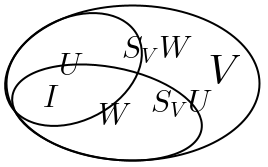
\includegraphics[width=80pt]{diagram3F-1}$\\\;\\\;}$\par\vspace{-42pt}\quad
%Now $0\neq x\in S_V I\Rightarrow\exists\,!\,\Par{u_v,i_u,w_v,i_w}\in S_V U\times S_U I\times S_V W\times S_W I,$\par\quad
%$x=u_v+i_u=w_v+i_w.$ Define $\varphi\in U^0,\beta\in W^0$ by $\varphi:u_v\mapsto 1,u\mapsto 0,$ and $\beta:i_u\mapsto 1,i\mapsto 0,$\par\quad
%for all $u\in\Pure V\XSlash\Span{u_v}$ and $i\in\Pure V\XSlash\Span{i_u}.$ \OR Define $\psi\in W^0,\gamma\in U^0,$ simlr.\par\quad
%Then $\varphi=\varphi+\beta=\psi+\gamma\in U^0+W^0.$\PfEnd
\AComm Not true if $U$ or $W$ is merely a subset. Promote $U\cap W$ as $I,$ \,$U$ as $X,$ \,and $W$ as $Y.$\par
%Now we show $X\cap Y=I.$ So that $\BigPar{U\cap W}{^0}=I^0=\BigPar{X\cap Y}{^0}=X^0+Y^0=U^0+W^0.$\parCom
\AExa Let $U=\Bra{\Par{x,x+1}\in\Rbb^2},W=\Rbb^2.$ Then $U\cap W=I=U\neq\Rbb^2=X\cap Y.$
\SepLine
\pagebreak

\Anchor{3FT1}\ProblemBX{\TipsN{1}}{
	\TextB{Prove $V=U\oplus W\Longleftrightarrow V\apostrophe=U^0\oplus W^0.$}
}$U\cap W=\zeroSubs\Longleftrightarrow \BigPar{U\cap W}{^0}=\zeroSubs{_V^0}=V\apostrophe=U^0+W^0.$\parSol{\vspace{1pt}}
$V=U+W\Longleftrightarrow\BigPar{U+W}{^0}=V_V^0=\zeroSubs=U^0\cap W^0.$\PfEnd
\SepLine

\Anchor{3F'3}\ProblemB{
	\TextB{Supp $V=U\oplus W$. Define $\iota:V\rightarrow U$ by $\iota\Par{u+w}=u.$ Thus $\iota\apostrophe\in\Lm{U\apostrophe,V\apostrophe}.$\vspace{2pt}}
	\PrePa\TextB{Show $\null \iota\apostrophe=\zeroSubs$\hspace{1pt}$:${\tgnr\FontNorm\;\;$\null\iota\apostrophe=\Par{\range\iota}{^0_U}=U_U^0=\zeroSubs.$\;\Or $\iota\apostrophe\Par{\psi}=\psi\circ\iota=0\Longleftrightarrow U\subseteq\null\psi.$}\vspace{2pt}}
	\PrePb\TextB{Prove $\range\iota\apostrophe=W_V^0$\hspace{1pt}$:${\tgnr\FontNorm\;\;$\range\iota\apostrophe=\BigPar{\null\iota}{^0_V}=W_V^0.$ \:\:Now $\tilde{\iota\apostrophe}$ is iso from $U\apostrophe\XSlash{\envFontDefault\zeroSubs}$ onto $W^0$}\vspace{0pt}}
}(b) \Or Note that $W=\null{\iota}\subseteq\Null\Par{\psi\circ\iota}.$ Then $\psi\circ\iota\in W^0\Rightarrow\range\iota\apostrophe\in W^0.$\parSol{\Hb}
\Blind{\Or}Supp $\varphi\in W^0.$ Becs $\null\iota=W\subseteq\null\varphi.$ By \Sbra{3.B \TIPSN{3}}, $\varphi=\varphi\circ\iota=\iota\apostrophe\Par{\varphi}.$\PfEnd
\SepLine

\Anchor{3F'4}\ProblemB{
	\TextB{Supp $V=U\oplus W.$ Prove $U^0=\Bra{\varphi\in V\apostrophe:\varphi=\varphi\circ\iota},$ \FontNorm where $\iota\in\Lm{V,W}:u_v+w_v\rightarrow w_v$.}
%	\NewNotation\;\;Denote $W^0$ by $U_V\upapostrophe,$ and $U^0$ by $W_V\upapostrophe.$\TextB{}
}$\varphi\in U^0\Longleftrightarrow U\subseteq\null\varphi\Longleftrightarrow\varphi=\varphi\circ\iota,$ by \Sbra{3.B \TIPSN{3}}.\PfEnd\vspace{3pt}
\ANote The nota $W_V\upapostrophe=\Bra{\varphi\in V\apostrophe:\varphi=\varphi\circ\iota}=U^0$ is not well-defined \Sbra{without a bss}.\parNot
Simply becs $W_V\upapostrophe$ have no info about the given $U.$ Here is an informal explanation:\parNot
Each liney map $T\in\Lm{V,W}$ that vanishes on a given nontrivial $U$ has its '$P$'\parNot
\Par{ though not uniq } suth '$U\oplus P=V$' with $T:P\mapsto\range T$ being surj.\parNot
Hence $\forall W\in\Scom{V}{U},\,U^0=W_{V}'.$ But given nontrivial '$P$', the corres '$U$' is not uniq.\parNot
Fix one $W_V\upapostrophe,$ then $U^0$ is not uniq, with each $U_k$ not equal to each other while each $U_k^0=W_V\upapostrophe.$\par\vspace{2pt}
\AExa Let $B_V=\Par{e_1,e_2}.$ Let $B_U=\Par{e_1},B_X=\Par{e_2-e_1},B_Y=\Par{e_2}.$\parExa
Then $\iota_X:ae_1+b\Par{e_2-e_1}\mapsto b\Par{e_2-e_1},\;\;\iota_Y:ae_1+be_2\mapsto be_2.$ Now $X_V\upapostrophe=Y_V\upapostrophe=U^0.$\parExa
(1) For $V=U\oplus X,$ let $B_{U_V'}=\Par{\varphi}$ with $\varphi:e_1\mapsto 1,\;e_2-e_1\mapsto 0\Rightarrow e_2\mapsto 1.$\parExa
(2) For $V=U\oplus Y,$ let $B_{U_V'}=\Par{\psi}$ with $\psi:e_1\mapsto 1,e_2\mapsto 0.$\parExa
Thus $X^0=U_V\upapostrophe$ while $Y^0=U_V\upapostrophe\Rightarrow X^0=Y^0\Rightarrow X=Y,$ ctradic.\parExa
To fix this, we must have a bss of $V\apostrophe$ as precond, which we'll see in the {\NOTEFOR} Exa (31).\par\vspace{2pt}
\ANote {\tgsl Supp $U$ is a subsp of $V.$ Then finding the corres subsp in $V\apostrophe$ firstly req another 'half' $W\in\Scom{V}{U},$}\vspace{-2pt}\parNot
{\tgsl while finding the corres subsp of $V$ for a subsp of $V\apostrophe$ must have the another 'half' asumed as precond.}
\SepLine

\ProblemN{\Anchor{3F31}{31}}{
	\TextA{Supp $V$ is finide and $B_{V\apostrophe}=\Par{\varphi_1,\dots,\varphi_n}.$ Show $\exists\,!\,B_V$ whose dual bss is the $B_{V\apostrophe}$.}
}For each $k\in\Bra{1,\dots,n},$ let $\Gamma_{\!k}=\Bra{1,\dots,n}\Backslash[\Big]\Bra{k}.$ Let each $U_k=\bigcap_{j\in\Gamma}\null\varphi_j.$\parSol{}
By Exe (4E 23), $V\apostrophe=\Span{\varphi_1,\dots,\varphi_n}=\BigPar{\null\varphi_1\cap\cdots\cap\null\varphi_n}{^0}\Rightarrow U_k\cap\varphi_k=\zeroSubs.$\parSol{}
Thus $\forall x_k\in U_k\nonzero,\;x_k\not\in\null\varphi_k$ while $x_k\in\null\varphi_j$ for all $j\in\Gamma.$\parSol{}
Fix one $x_k$ and let $v_k=\Sbra{\varphi_k\Par{x_k}}{^{-1}}x_k\Rightarrow\varphi_k\Par{v_k}=1,\,\varphi_j\Par{v_k}=0$ for all $j\neq k.$\parSol{}
Simply for each $v_k,$ \,$\varphi_j\Par{v_k}=\delta_{j,k}$ for all $j\Longleftrightarrow$ for each $\varphi_j,$ $\varphi_j\Par{v_k}=\delta_{j,k}$ for all $k.$\parSol{}
又 $a_1v_1+\dots+a_nv_n=0\Rightarrow$ each $\varphi_k\Par{0}=a_k.$\vspace{2pt}\parSol{}
Now we prove the uniqnes part. Supp the dual bss of $B_V'=\Par{u_1,\dots,u_n}$ is the $B_{V\apostrophe}.$\parSol{}
For each $k,$ we have $\varphi_j\Par{v_k}=\varphi_j\Par{u_k}$ for all $k\Rightarrow v_k-u_k\in\bigcap\null\varphi_j=\zeroSubs.$\PfEnd
\SepLine

\Anchor{3FN31}\BulletPointX\NoteForSmall{Exe (31)}\;\;Supp $V$ is finide, and $\Omega$ is a subsp of $V\apostrophe$ with $B_{\Omega}=\Par{\varphi_1,\dots,\varphi_m}.$\TextB{}
The '$W$' is not clear when we are to find suth $W_V\apostrophe=\Omega,$ becs the another 'half' is undefined.\TextB{}
Extend to $B_{V\apostrophe}=\Par{\varphi_1,\dots,\varphi_n}.$ By Exe (31), $\exists\,!\,$corres $B_V=\Par{v_1,\dots,v_n}.$\TextB{}
Let $B_U=\Par{v_{m+1},\dots,v_n},B_W=\Par{v_1,\dots,v_m}.$ \,Thus we found the $W$ suth $\Omega=W_V\upapostrophe,$\TextB{}
which is well-defined with $B_V$ as precond.
\SepLine
\pagebreak

\Anchor{3FT2}\BulletPointX\TipsN{2}\,\,\,Supp $\varphi_1,\dots,\varphi_m\in V\apostrophe.$ Denote $\Sbra{\null\psi_a\cap\cdots\cap\null\varphi_b}$ by \,$\bigcap_a^b\null\varphi_I.$\TextB{}
\IndentTipsN{2}Supp $\Omega$ is a subsp of $V\apostrophe.$ Denote $\Bra{v\in V:\varphi\Par{v}=0,\forall\varphi\in\Omega}$ by $C^0\,\Omega.$\TextB{\vspace{1pt}}
If $\Omega$ is infinide, then by def, $\bigcap_{\in\,\Omega}\null\varphi=C^0\,\Omega.$ \; If $\Omega=\Span{\varphi_1,\dots,\varphi_m},$\TextB{}
then $v\in\bigcap_1^m\null\varphi_I\Longleftrightarrow$ each $\varphi_k\Par{v}=0\Longleftrightarrow\forall\varphi=\sum_{i=1}^na_i\varphi_i\in\Omega,\varphi\Par{v}=0\Longleftrightarrow v\in C^0\,\Omega.$
\SepLine

\Anchor{3F4e23}\ProblemBnoor{{4E 23}}{
	\TextB{Supp $V$ is finide, $\Omega=\Span{\varphi_1,\dots,\varphi_m}\subseteq V\apostrophe.$ Prove $\Omega=\BigPar{\null\varphi_1\cap\cdots\cap\null\varphi_m}{^0}.$}
}Becs each $\Span{\varphi_k}\subseteq\Par{\null\varphi_k}{^0}.$ By {\NOTEFOR} Exe (1) and Exe (23), Immed.\PfEnd\parSol{\vspace{4pt}}
\Or Reduce to $B_{\Omega}=\Par{\beta_1,\dots,\beta_p}.$ We show $\Omega=\Par{\null\beta_1\cap\cdots\cap\null\beta_p}{^0},$ then done by \TIPSN{3}.\parSol{}
Let $B_{V\apostrophe}=\Par{\beta_1,\dots,\beta_p,\gamma_1,\dots,\gamma_q}.$ By Exe (31), let $B_V=\Par{v_1,\dots,v_p,u_1,\dots,u_q}.$\parSol{}
Define each $\Gamma_{\!k}=\Bra{1,\dots,p}\Backslash[\Big]\Bra{k}.$ Then $\null\beta_k=\Span[\Bra]{v_j}{_{j\,\in\,\Gamma_{\!k}}}\oplus\Span{u_1,\dots,u_q}.$\parSol{}
Now $\Par{\null\beta_1\cap\cdots\cap\null\beta_p}=\Span{u_1,\dots,u_q}.$ Simlr to (4E 2.C.16).\parSol{}
Supp $\varphi=\sum_{i=1}^pa_i\beta_i+\sum_{j=1}^qb_j\gamma_j\in\Span{u_1,\dots,u_q}{^0}.$ Then each $\varphi\Par{u_k}=0=b_k$\parSol{}
Thus $\Span{u_1,\dots,u_q}{^0}\subseteq\Span{\beta_1,\dots,\beta_p}=\Omega.$\PfEnd
\SepLine

\Anchor{3FT3}\ProblemBX{\TipsN{3}}{
	\TextA{Supp each $\varphi_i,\beta_j\in\Lm{V,W}.$ Supp $\Span{\varphi_1,\dots,\varphi_m}=\Span{\beta_1,\dots,\beta_n}.$}
	\TextA{Prove $\null\varphi_1\cap\dots\cap\null\varphi_m=\null\beta_1\cap\dots\cap\null\beta_n.$\vspace{0pt}}
}Becs each $\beta_k\in\Span{\varphi_1,\dots,\varphi_m}.$\parSol{}
$\forall v\in\bigcap_1^m\null\varphi_I,\beta_k\Par{v}=0.$ Thus $\bigcap_1^m\null\varphi_I\subseteq\bigcap_1^n\null\beta_I.$ \;Rev the roles and done.\PfEnd\vspace{2pt}
\ANote Supp $\varphi_j=c_1\varphi_1+\dots+c_{j-1}\varphi_{j-1}.$\parNot{\vspace{2pt}}
Let $N_j\oplus\bigcap_1^{j-1}\null\varphi_I=\null\varphi_j.$ Now $\bigcap_1^j\null\varphi_I=\bigcap_1^{j-1}\null\varphi_I\cap\BigPar{\null\varphi_j}=\bigcap_1^{j-1}\null\varphi_I.$\parNot{\vspace{2pt}}
Thus $\bigcap_1^m\null\varphi_I=\Sbra{\bigcap_1^{j-1}\null\varphi_I}\cap\Sbra{\bigcap_{j+1}^m\null\varphi_I}.$ \;Hence $\bigcap_1^n\null\beta_I=\bigcap_{1}^m\null\varphi_I.$
\SepLine

\ProblemN{\Anchor{3F26}{26}}{
	\TextB{Supp $V$ is finide, $\Omega$ is a subsp of $V\apostrophe.$ Prove $\Omega=\BigPar{C^0\,\Omega}{^0}.$}
}Let $B_{\Omega}=\Par{\varphi_1,\dots,\varphi_m}.$ By {\TIPSN{2}} and Exe (4E 23).\PfEnd\vspace{1pt}
\AExa Immed, $\Omega\subseteq\Par{C^0\,\Omega}{^0}.$ Now we give a countexa for $\Omega\supseteq\Par{C^0\,\Omega}{^0}.$\parExa
Let $V=\Bra{\Par{x_1,x_2,\cdots}\in\Fbb^{\infty}:x_k\neq 0\text{ for only finily many }k}.$ Then $V\apostrophe=\Par{\Fbb^{\infty}}\apostrophe.$\parExa
Let $\Omega=\Bra[\envFontA]{\varphi\in\Span{\varphi_{\alpha_1},\dots,\varphi_{\alpha_m}}:\exists\:m,\alpha_k\in\Nbp}\subsetneq V\apostrophe.$ Then $C^0\,\Omega=\zeroSubs\Rightarrow\Par{C^0\,\Omega}{^0}=V\apostrophe.$\par\vspace{2pt}
\ACoro (1) $C^0\,\Span{\varphi_1,\dots,\varphi_m}=\null\varphi_1\cap\cdots\cap\null\varphi_m.$\parCor
(2) Supp $V$ is finide. For every subsp $\Omega$ of $V\apostrophe,\;\exists\,!\,$subsp $U$ of $V$ suth $\Omega=U^0.$\vspace{-2pt}\parCor
\Blind{(2)} {\FontSmall\tgsl This form of $\Omega$ does not depend on a bss and thus is considered more general.}\vspace{-2pt}\par
\SepLine

\Anchor{3F'5}\ProblemB{
	\TextB{Supp $\Span{\varphi_1,\dots,\varphi_m}\subseteq V\apostrophe.$ Let each $U_k\oplus\null\varphi_k=V.$}
	\TextB{Prove or give a countexa\hspace{1pt}$:$ $\Par{U_1+\dots+U_m}\oplus\BigPar{\null\varphi_1\cap\cdots\cap\null\varphi_m}=V.$}
}Let $V=\Rbb^2.$ Define $\varphi_1=\varphi_2:\Par{x,y}\mapsto x.$ Let $B_{U_1}=\Par{e_1},B_{U_2}=\Par{e_1+e_2}\Rightarrow U_1+U_2=V.$\parSol{}
\Or Let $B_{V\apostrophe}=\Par{\varphi_1,\varphi_2}$ be corres to the std bss. Let $B_{U_1}=B_{U_2}=\Par{e_1+e_2}\Rightarrow U_1+U_2\subsetneq V.$\PfEnd
\SepLine

\Anchor{3FT4}\ProblemBX[]{\TipsN{4}}{
	Let $B_{U^0}=\Par{\varphi_1,\dots,\varphi_m},B_{V\apostrophe}=\Par{\varphi_1,\dots,\varphi_n}\Rightarrow B_V=\Par{v_1,\dots,v_n}.$\TextA{}
	We show (a) $B_U=\Par{v_{m+1},\dots,v_n};$ \;(b) $U=\null\varphi_1\cap\cdots\cap\null\varphi_m.$\TextA{}
	(a) Becs $\Span{v_{m+1},\dots,v_n}{^0}=\Span{\varphi_1,\dots,\varphi_m}=U^0.$ Now by Exe (20, 21).\TextA{}
	\Ha\Or Becs by (b), $U=\bigcap_1^m\null\varphi_I=\Span{v_{m+1},\dots,v_n}.$\vspace{2pt}\TextA{}
	(b) Each $\null\varphi_k=\Span[\Bra]{B_V\Backslash\Bra[\envFontB]{v_k}}\Rightarrow\bigcap_1^m\null\varphi_I=\Span{v_{m+1},\dots,v_n}.$ Now by (a).\TextA{}
	\Hb\Or Becs $\Span{\varphi_1,\dots,\varphi_m}=U^0=\BigPar{\null\varphi_1\cap\cdots\cap\null\varphi_m}{^0}.$ Now by Exe (20, 21).\PfEnd\TextA{\vspace{-3pt}}
}\SepLine\pagebreak

\ProblemN{\Anchor{3F24}{24}}{
	\TextA{Prove, using the pattern of [3.104], that $\dim U+\dim U^0=\dim V$.}
}By \TIPSN{4}. \;\Or Let $B_U=\Par{u_1,\dots,u_m},B_V=\Par{u_1,\dots,u_m,v_1,\dots,v_n},B_{V\apostrophe}=\Par{\psi_1,\dots,\psi_m,\varphi_1,\dots,\varphi_n}.$\parSol{}
Supp $\psi=\sum_{i=1}^ma_i\psi_i+\sum_{j=1}^nb_j\varphi_j\in U^0\Rightarrow$ each $\psi\Par{u_k}=a_k=0.$ Thus $U^0\subseteq\Span{\varphi_1,\dots,\varphi_n}.$\PfEnd
\SepLine

\Anchor{3F28}\Anchor{3F29}\ProblemB{
	\TextB{Supp $T\in\Lm{V,W},$ each $\varphi_k\in V\apostrophe,$ and each $\psi_k\in W\apostrophe.$}
	\ProblemN[]{}{}
	\ProblemN[]{28}{
		\TextA{Prove $\null T\apostrophe=\Span{\psi_1,\dots,\psi_m}\Longleftrightarrow\range T=\Par{\null\psi_1}\cap\cdots\cap\Par{\null\psi_m}.$}}
	\ProblemN[]{29}{
		\TextA{Prove $\range T\apostrophe=\Span{\varphi_1,\dots,\varphi_m}\Longleftrightarrow\null T=\Par{\null\varphi_1}\cap\cdots\cap\Par{\null\varphi_m}.$}}
	\TextB{\vspace{-4pt}}
}$\Par{\range T}{^0}=\null T\apostrophe=\Span{\psi_1,\dots,\psi_m}=\BigPar{{\null\psi_1}\cap\cdots\cap{\null\psi_m}}{^0}.$\parSol{}
$\Par{\null T}{^0}=\range T\apostrophe=\Span{\varphi_1,\dots,\varphi_m}=\BigPar{{\null\varphi_1}\cap\cdots\cap{\null\varphi_m}}{^0}.$\PfEnd
\SepLine

\ProblemN{\Anchor{3F34}{34}}{
%	\TextA{The double dual space of $V$, denoted by $V\apostrophe\apostrophe$, is defined  to be the dual space of $V\apostrophe$.}
%	\TextA{In other words, $V\apostrophe\apostrophe=\Lm{V\apostrophe,\Fbb}$. Define $\Lambda:V\rightarrow V\apostrophe\apostrophe$ by $\Par{\Lambda v}\Par{\varphi} = \varphi\Par{v}$.\vspace{2pt}}
	\TextA{Define $\Lambda:V\rightarrow \Fbb^{V\apostrophe}$ by $\Lambda v=\overline{v},$ and $\overline{v}:V\apostrophe\rightarrow\Fbb$ by $\overline{v}\Par{\varphi}=\varphi\Par{v}.$\vspace{2pt}}
	\PrePa\TextA{Show $\overline{v}\in V\apostrophe\apostrophe$ and $\Lambda\in\Lm{V,V\apostrophe\apostrophe}.$\vspace{2pt}}
	\PrePb\TextA{Show if $T\in\Lm{V}$, then $T\apostrophe\apostrophe\circ\Lambda=\Lambda\circ T$, where $T\apostrophe\apostrophe=\Par{T\apostrophe}\apostrophe$.\vspace{2pt}}
	\PrePc\TextA{Show if $V$ is finide, then {\tgsc $\Lambda$ is iso from $V$ onto $V\apostrophe\apostrophe$}.}
%	\TextA{\normalsize Supp $V$ is finide. Then $V$ and $V\apostrophe$ are iso, and finding iso from $V$ onto $V\apostrophe$ generally req choosing\vspace{-3pt}}
%	\TextA{\normalsize a bss of $V$. In contrast, the iso $\Lambda$ from $V$ onto $V\apostrophe\apostrophe$ does not req a choice of bss and thus is considered more natural.}
}(a) $\overline{v}\Par{\varphi+\lambda\psi}=\Par{\varphi+\lambda\psi}\Par{v}=\varphi\Par{v}+\lambda\psi\Par{v}=\overline{v}\Par{\varphi}+\lambda\overline{v}\Par{\psi}.$\parSol{\Ha}
$\overline{v+\lambda w}\Par{\varphi}=\varphi\Par{v+\lambda w}=\varphi\Par{v}+\lambda\varphi\Par{w}=\overline{v}\Par{\varphi}+\lambda\overline{w}\Par{\varphi}.$\vspace{2pt}\parSol{}
(b) $\BigPar{T\apostrophe\apostrophe\overline{v}}\Par{\varphi}=\BigPar{\overline{v}\circ{T\apostrophe}}\Par{\varphi}=\overline{v}\BigPar{T\apostrophe\Par{\varphi}}=\BigPar{T\apostrophe\Par{\varphi}}\Par{v}=\Par{\varphi\circ T}\Par{v}=\varphi\Par{Tv}=\overline{Tv}\Par{\varphi}.$\vspace{2pt}\parSol{}
(c) $\overline{v}=0\Rightarrow\forall\varphi\in V\apostrophe,\overline{v}\Par{\varphi}=\varphi\Par{v}=0\Rightarrow v=0.$ Inje. Now becs $V$ finide.\PfEnd\vspace{2pt}
\AComm Supp $\Phi\in V\apostrophe\apostrophe$ and $\Phi\neq 0.$ Then $\exists\,\varphi\in V\apostrophe,\:\Phi\Par{\varphi}=1\Rightarrow\null\Phi\oplus\Span{\varphi}=V\apostrophe.$\parCom
And $\varphi\neq 0\Rightarrow\exists\,v\in V,\:\varphi\Par{v}=1,\null\varphi\oplus\Span{v}=V.$ Becs $\Lambda$ is surj.\parCom
Now $\exists\,x\in V,\forall\psi=c\varphi+\rho\in V\apostrophe,\psi\Par{x}=\overline{x}\Par{\psi}=\Phi\Par{\psi}=c.$
\SepLine

\ProblemN{\Anchor{3F36}{36}}{
	\TextA{Supp $U$ is a subsp of $V$. Define $i:U\rightarrow V$  by $i\Par{u}=u$. Thus $i\apostrophe\in\Lm{V\apostrophe,U\apostrophe}.$\vspace{2pt}}
	\PrePa\TextA{Show $\nullp i\apostrophe=U^0$\hspace{1pt}$:${\tgnr\FontNorm\;\;$\nullp i\apostrophe=\Par{\rangep i}{^0}=U^0\Leftarrow\rangep i=U$.}\vspace{2pt}}
	\PrePb\TextA{Prove $\rangep i\apostrophe=U\apostrophe$\hspace{1pt}$:${\tgnr\FontNorm\;\;$\rangep i\apostrophe=\Par{\nullp i}{_U^0}={\zeroSubs}{_U^0}=U\apostrophe$.}\vspace{2pt}}
	\PrePc\TextA{Prove $\tilde{i\apostrophe}$ is iso from $V\apostrophe\XSlash U^0$ onto $U\apostrophe$\hspace{1pt}$:${\tgnr\FontNorm\;\;Immed.}\vspace{1pt}}
}(a) \Or $\forall\varphi\in V\apostrophe,i\apostrophe\Par{\varphi}=\varphi\circ i=\varphi\mmid_U.$ Thus $i\apostrophe\Par{\varphi}=0\Longleftrightarrow\forall u\in U,\varphi\Par{u}=0\Longleftrightarrow\varphi\in U^0.$\parSol{}
(b) \Or Supp $\psi\in U\apostrophe.$ By (3.A.11), $\exists\,\varphi\in V\apostrophe,\varphi\mmid_U=\psi.$ Then $i\apostrophe\Par{\varphi}=\psi.$\PfEnd
\SepLine

\Anchor{3FN3.109b}\ProblemB{
	\TextB{Supp $T\in\Lm{V,W}.$ Prove $\range T\apostrophe\supseteq\BigPar{\null T}{^0}.$\hfill\Sbra[3pt]{{\tgsc\large Another proof of \tgnr\tgbfx[3.109](b)}}\vspace{1pt}}
}Let $V=U\oplus\null T.$ Let $R=\Par{T\mmid_U}{^{-1}}\Big|{_{\range T}}.$ Define $\iota\in\Lm{V,U}$ by $\iota\Par{u+w}=u.$\vspace{1pt}\parSol{}
$\forall\varPhi\in\BigPar{\null T}{^0},$ let $\psi=\varPhi\circ R,$ then $T\apostrophe\Par{\psi}=\psi\circ T=\varPhi\circ\BigPar{R\circ T\mmid_V}=\varPhi\circ\iota=\varPhi\in\range T\apostrophe.$\PfEnd\vspace{2pt}\Anchor{3F4e17}
\ACoro [3.108] and [3.110] hold without the hypo of finide. Now $T$ inv $\Longleftrightarrow T\apostrophe$ inv.
\SepLine

\Anchor{3F12}\ProblemN[]{12}{
	\TextA{{\large\tgnr Note that $I_{V}\upapostrophe,I_{V\apostrophe}:V\apostrophe\rightarrow V\apostrophe.$} \,For $\varphi\in V\apostrophe,\:I_{V\apostrophe}\Par{\varphi}=\varphi=\varphi\circ I_V=I_V\upapostrophe\Par{\varphi}.$ Thus $I_{V\apostrophe}=I_V\upapostrophe.$}
}\SepLine

\ProblemN{\Anchor{3F15}{15}}{
	\TextA{Supp $T\in\Lm{V,W}$. Prove $T\apostrophe=0\Rightarrow T=0.$ \hfill\tgnr\FontNorm\ACoro If $V,W$ finide, then $\Gamma:T\mapsto T\apostrophe$ is iso.}
}Supp $T\apostrophe=0.$ Then $\Par{\range T}{^0}=\null T\apostrophe=W\apostrophe.$\parSol{}
By Exe (25), $\range T=\Bra{w\in W:\varphi\Par{w}=0,\forall\varphi\in\Par{\range T}{^0}=W\apostrophe}.$\parSol{}
Asum $w\neq 0$ suth $\forall\varphi\in W\apostrophe,\varphi\Par{w}=0.$ Let $U\oplus\Span{w}=W.$\parSol{}
Define $\psi\in W\apostrophe$ by $\psi\Par{u+\lambda w}=\lambda\Rightarrow\psi\Par{w}\neq 0.$ Ctradic. Now $\range T=\zeroSubs.$\PfEnd
\SepLine

\Anchor{3FN16}\BulletPointX\NoteForSmall{Exe (16)}\vspace{-2pt}\TextB{}
%{\FontSmall Let $B_{\range\mT}=\Par{\varphi_1,\dots,\varphi_p}$ with each $\varphi_k=\mT\psi_k. $ Let $B_{V\apostrophe}=\Par{\varphi_1,\dots,\varphi_p,\gamma_1,\dots,\gamma_q}\Rightarrow B_V=\Par{v_1,\dots,v_p,u_1,\dots,u_q}.$}\vspace{-3pt}\TextB{}
%{\FontSmall Let $B_{\null\mT}=\Par{\beta_1,\dots,\beta_l}\Rightarrow B_{W\apostrophe}=\Par{\psi_1,\dots,\psi_p,\beta_1,\dots,\beta_r}\Rightarrow B_W=\Par{w_1,\dots,w_p,x_1,\dots,x_r}.$}\TextB{}
%Let $A^t=\Mt[\BigPar]{\mT,B_{W\apostrophe},B_{V\apostrophe}}.$ Then $A^t_{i,j}=0,A^t_{k,k}=1$ for all $i\neq j$ and each $1\leqslant k\leqslant p.$\TextB{}
%Define $T$ with each $Tv_i=w_i$ and each $Tu_j=0.$ Then each $T\apostrophe\Par{\beta_k}=0=\mT\beta_k.$\TextB{}
%And each $\Sbra{T\apostrophe\Par{\psi_j}}\Par{v}=\psi_j\Par{a_1w_1+\dots+a_pw_p}=a_j=\varphi_j\Par{v}={\mT\psi_j}\Par{v}.$ \;Now by Exe (16).\vspace{4pt}\TextB{}
{\FontSmall Let $B_V=\Par{v_1,\dots,v_n},B_{V\apostrophe}=\Par{\varphi_1,\dots,\varphi_n},B_W=\Par{w_1,\dots,w_m},B_{W\apostrophe}=\Par{\psi_1,\dots,\psi_m}.$}\TextB{}
Define each $E_{j,k}\in\Lm{V,W}:v_x\mapsto\delta_{j,x}w_k,$ and each $\reflectbox{\textit{E}}{_{k,j}}\in\Lm{W\apostrophe,V\apostrophe}:\psi_x\mapsto\delta_{k,x}\varphi_j.$\TextB{}
Note that each $E_{j,k}\!\!\upapostrophe\,\,\Par{\psi_x}=\psi_x\circ E_{j,k}=\delta_{k,x}\varphi_j=\reflectbox{\textit{E}}{_{k,j}}\Par{\psi_x}\Rightarrow E_{j,k}\!\!\upapostrophe\,\,=\reflectbox{\textit{E}}{_{k,j}}.$\vspace{1pt}\TextB{}
$\Lm{V,W}\ni T=\sum_{j=1}^n\sum_{k=1}^mA_{k,j}E_{j,k}\Longleftrightarrow\mT=\sum_{j=1}^n\sum_{k=1}^mA_{k,j}\reflectbox{\textit{E}}{_{k,j}}\in\Lm{W\apostrophe,V\apostrophe}.$ Uniqly by Exe (16).\vspace{3pt}\Anchor{5E5}\TextB{}
\ACoro $ST=TS\Longleftrightarrow S\apostrophe T\apostrophe=T\apostrophe S\apostrophe.$ \;By Exe (16). \Or Becs $AC=CA\Longleftrightarrow A^tC^t=C^tA^t.$
\SepLine

\Anchor{3F4e8}\ProblemBnoor{{4E 8}}{
	\TextB{Describe the relation of $B_V=\Par{v_1,\dots,v_{n}}$ and the corres $B_{V\apostrophe}=\Par{\varphi_1,\dots,\varphi_{n}}$ using isos.}
}Define $\Gamma:V\rightarrow\Fbb^n$ by $\Gamma\Par{v}=\BigPar{\varphi_1\Par{v},\dots,\varphi_{n}\Par{v}},$ and
$\Gamma^{-1}\Par{a_1,\dots,a_n}=a_1v_1+\dots+a_nv_n.$\PfEnd
\SepLine

\ProblemN{\Anchor{3F4e24}\Anchor{3F6}{6}}{
	\TextA{Define \,$\Gamma: V\apostrophe\rightarrow\Fbb^m\,$ by $\,\Gamma\Par{\varphi}=\BigPar{\varphi\Par{v_1},\dots,\varphi\Par{v_m}},$ where $v_1,\dots,v_m\in V$.}
	\PrePa\TextA{Show $\Span{v_1,\dots,v_m}=V\,\Longleftrightarrow \Gamma$ is inje.}
	\PrePb\TextA{Show $\Par{v_1,\dots,v_m}$ is liney indep $\Longleftrightarrow \Gamma$ is surj.}
}Let $\Par{e_1,\dots,e_m}$ be the std bss of $\Fbb^m.$\par\quad
(a) Becs $\Gamma\Par{\varphi}=0\Longleftrightarrow\varphi\Par{v_1}=\dots=\varphi\Par{v_m}=0\Longleftrightarrow\null\varphi=\Span{v_1,\dots,v_m}.$ Immed.\vspace{1pt}\par\quad
(b) Supp $\Gamma$ is surj. Let each $e_k=\Gamma\Par{\varphi_k}\Rightarrow\varphi_k\Par{v_j}=\delta_{j,k}.$ Now $a_1v_1+\dots+a_mv_m=0\Rightarrow$ each $a_k=\varphi_k\Par{0}.$\vspace{1pt}\par\quad\Hb
Supp $\Par{v_1,\dots,v_m}$ is liney indep. Let $U=\Span{v_1,\dots,v_m},B_{U\apostrophe}=\Par{\psi_1,\dots,\psi_m}.$ Let $W\oplus U=V.$\par\quad\Hb
Define $\iota:u_v+w_v\mapsto u_v.$ Each $\psi_k\circ\iota=\varphi_k\in V\apostrophe\Rightarrow\varphi_k\Par{v_j}=\psi_k\Par{v_j}=\delta_{j,k}\Rightarrow$ each $e_k=\Gamma\Par{\varphi_k}.$\PfEnd\vspace{4pt}\quad
\Or Let $\Par{\psi_1,\dots,\psi_m}$ be dual bss of the std bss of $\Fbb^m.$ Define an iso $\Psi:\Fbb^m\rightarrow\Par{\Fbb^m}\apostrophe$ by $\Psi\Par{e_k}=\psi_k.$\par\quad
Define $T\in\Lm{\Fbb^m,V}$ by $Te_k=v_k.$ Now $T\Par{x_1,\dots,x_m}=T\Par{x_1e_1+\dots+x_me_m}=x_1v_1+\dots+x_mv_m.$\par\quad
$\forall\varphi\in V\apostrophe,k\in\Bra{1,\dots,m},\Sbra{T\apostrophe\Par{\varphi}}\Par{e_k}=\varphi\Par{Te_k}=\varphi\Par{v_k}=\Sbra{\varphi\Par{v_1}\psi_1+\dots+\varphi\Par{v_m}\psi_m}\Par{e_k}$\par\quad
Now $T\apostrophe\Par{\varphi}=\varphi\Par{v_1}\psi_1+\dots+\varphi\Par{v_m}\psi_m=\Psi\BigPar{\varphi\Par{v_1},\dots,\varphi\Par{v_m}}=\Psi\BigPar{\Gamma\Par{\varphi}}.$ Hence $T\apostrophe=\Psi\circ\Gamma.$\par\quad
By (3.B.3),
(a) $\range T=\Span{v_1,\dots,v_m}=V\Longleftrightarrow T\apostrophe$ inje $\Longleftrightarrow\Gamma$ inje.\par\quad
\Blind{By (3.B.3),} (b) $\Par{v_1,\dots,v_m}$ is liney indep $\Longleftrightarrow T$ is inje $\Longleftrightarrow T\apostrophe$ surj $\Longleftrightarrow\Gamma$ surj.\PfEnd
\SepLine

\Anchor{3F4e25}\ProblemBnoor{{4E 25}}{
	\TextB{Define \,$\Gamma: V\rightarrow\Fbb^m\,$ by $\,\Gamma\Par{v}=\BigPar{\varphi_1\Par{v},\dots,\varphi_m\Par{v}},$ where $\varphi_1,\dots,\varphi_m\in V\apostrophe.$}
	(c) \TextB{Show $\Span{\varphi_1,\dots,\varphi_m}=V\apostrophe\,\Longleftrightarrow \Gamma$ is inje.}
	(d) \TextB{Show $\Par{\varphi_1,\dots,\varphi_m}$ is liney indep $\Longleftrightarrow \Gamma$ is surj.}
}Let $\Par{e_1,\dots,e_m}$ be the std bss of $\Fbb^m.$\par\quad
(c) Becs $\Gamma\Par{v}=0\Longleftrightarrow\varphi_1\Par{v}=\dots=\varphi_m\Par{v}=0\Longleftrightarrow v\in\Par{\null \varphi_1}\cap\dots\cap\Par{\null\varphi_m}.$\par\quad\Hc
By Exe (4E 23), $\Span{\varphi_1,\dots,\varphi_m}=V\apostrophe\Longleftrightarrow\null\Gamma=\Par{\null \varphi_1}\cap\dots\cap\Par{\null\varphi_m}=\zeroSubs.$\par\quad
(d) Supp $\Par{\varphi_1,\dots,\varphi_m}$ is liney indep. \Sbra[3pt]{{\tgsl Req Finide}} \;Extend to $B_{V\apostrophe}=\Par{\varphi_1,\dots,\varphi_n}.$\par\quad\Hb
Then by Exe (31), $B_V=\Par{v_1,\dots,v_n}$ and each $\varphi_k\Par{v_j}=\delta_{j,k}\Rightarrow$ each $e_k=\Gamma\Par{\varphi_k}.$\par\quad\Hd
Supp $\Gamma$ is surj. Let each $e_k=\Gamma\Par{v_k}=\BigPar{\varphi_1\Par{v_k},\dots,\varphi_m\Par{v_k}}.$\par\quad\Hd
Now $a_1\varphi_1+\dots+a_m\varphi_m=0\Rightarrow$ each $a_k=0\Par{v_k}.$\par\quad\Hd
\Or Let $U=\Span{v_1,\dots,v_m}.$ Then $B_{U\apostrophe}=\BigPar{\varphi_1\Big|{_U},\dots,\varphi_m\Big|{_U}}\Rightarrow\Par{\varphi_1,\dots,\varphi_m}$ liney indep.\PfEnd\vspace{8pt}\quad
\Or Let $\Par{\psi_1,\dots,\psi_m}$ be dual bss of the std bss of $\Fbb^m.$ Define an iso $\Psi:\Fbb^m\rightarrow\Par{\Fbb^m}\apostrophe$ by $\Psi\Par{e_k}=\psi_k.$\par\quad
$\forall\Par{x_1,\dots,x_m}\in\Fbb^m,\Gamma\apostrophe\BigPar{\Psi\Par{x_1,\dots,x_m}}=\Par{x_1\psi_1+\dots+x_m\psi_m}\circ\Gamma.$\par\quad
$\forall v\in V,\Sbra{\Gamma\apostrophe\BigPar{\Psi\Par{x_1,\dots,x_m}}}\Par{v}=\Sbra{x_1\psi_1+\dots+x_m\psi_m}\BigPar{\varphi_1\Par{v},\dots,\varphi_m\Par{v}}=x_1\varphi_1\Par{v}+\dots+x_m\varphi_m\Par{v}.$\vspace{1pt}\par\quad
Now $\Gamma\apostrophe\BigPar{\Psi\Par{x_1,\dots,x_m}}=x_1\varphi_1+\dots+x_m\varphi_m.$ Define $\Phi:\Fbb^m\rightarrow V\apostrophe$ by $\Phi=\Gamma\apostrophe\circ\Psi.$ Thus by (3.B.3),\par\quad
(c) $\Gamma$ inje $\Longleftrightarrow\Gamma\apostrophe$ surj $\Longleftrightarrow\Phi$ surj $\Longleftrightarrow\Par{\varphi_1,\dots,\varphi_m}$ spanning $V\apostrophe.$\par\quad
(d) $\Gamma$ surj $\Longleftrightarrow\Gamma\apostrophe$ inje $\Longleftrightarrow\Phi$ inje $\Longleftrightarrow\Par{\varphi_1,\dots,\varphi_m}$ being liney indep.\PfEnd
\SepLine
\pagebreak

\ProblemN{\Anchor{3F9}{9}}{
	\TextA{Show $\forall\psi\in V\apostrophe,\psi=\psi\Par{v_1}\varphi_1+\dots+\psi\Par{v_n}\varphi_n,$ where $B_V=\Par{v_1,\dots,v_n},B_{V\apostrophe}=\Par{\varphi_1,\cdots,\varphi_n}.$}
}$\psi\Par{v}=a_1\psi\Par{v_1}+\dots+a_n\psi\Par{v_n}=\psi\Par{v_1}\varphi_1\Par{v}+\dots+\psi\Par{v_n}\varphi_n\Par{v}.$\PfEnd
\SepLine

\Anchor{3F13}\ProblemN[]{13}{
	\TextA{Define $T:\Rbb^3\!\rightarrow\!\Rbb^2$ by $T\Par{x,y,z}=\Par{4x+5y+6z,7x+8y+9z}$.\vspace{3pt}}
	\TextA{Let $\Par{\varphi_1,\varphi_2},\Par{\psi_1,\psi_2,\psi_3}$ denote the dual bss of std bss of $\Rbb^2$ and $\Rbb^3$.\vspace{4pt}}
	\PrePa\TextA{Describe the liney functionals $T\apostrophe\Par{\varphi_1},T\apostrophe\Par{\varphi_2}.$}
	\Blind{\PrePb}\TextA{{\FontNorm\tgnr For any $\Par{x,y,z}\in\Rbb^3$, $\BigPar{T\apostrophe\Par{\varphi_1}}\Par{x,y,z}=4x+5y+6z, \BigPar{T\apostrophe\Par{\varphi_2}}\Par{x,y,z}=7x+8y+9z$.}\vspace{6pt}}
	\PrePb\TextA{Write $T\apostrophe\Par{\varphi_1}$ and $T\apostrophe\Par{\varphi_2}$ as liney combinas of $\psi_1,\psi_2,\psi_3$.}
	\Blind{\PrePb}\TextA{{\FontNorm\tgnr$T\apostrophe\Par{\varphi_1}=4\psi_1+5\psi_2+6\psi_3,\,\,T\apostrophe\Par{\varphi_2}=7\psi_1+8\psi_2+9\psi_3.$}\vspace{6pt}}
	\PrePc\TextA{What is $\null T\apostrophe$? What is $\range T\apostrophe$?}
}\TextA{\vspace{4pt}}
\Hc $T\Par{x,y,z}=0\Longleftrightarrow\MathLeftBrace{l}{4x+5y+6z=0\\7x+8y+9z=0}\Longleftrightarrow\hMath{l}{\left\{}{\;\right|}{x=z,\\y=-2z.}\,\hText{$Thus $\null T=\Span{e_1-2e_2+e_3},\\$where $\Par{e_1,e_2,e_3}$ is std bss of $\Rbb^3.}$\vspace{4pt}\TextA{}
\Hc Let $\Par{e_1-2e_2+e_3,-2e_2,e_3}$ be a bss, with corres dual bss $\Par{\varepsilon_1,\varepsilon_2,\varepsilon_3}$.\vspace{1.5pt}\TextA{}
\Hc Thus $\Span{e_1-2e_2+e_3}=\null T\Rightarrow \Span{e_1-2e_2+e_3}{^0}=\Span{\varepsilon_2,\varepsilon_3}=\range T\apostrophe.$\vspace{1.5pt}\TextA{}
\Hc Note that $\varepsilon_k=\varepsilon_k\Par{e_1}\psi_1+\varepsilon_k\Par{e_2}\psi_2+\varepsilon_k\Par{e_3}\psi_3.$\vspace{1.5pt}\TextA{}
\Hc And $\MathLeftMid{l}{\varepsilon_2\Par{e_2}=-\frac{\;1\;}{2},\varepsilon_2\Par{e_1}=\varepsilon_2\Par{e_1-2e_2+e_3}+\varepsilon_2\Par{2e_2}-\varepsilon_2\Par{e_3}=1,\\[1.5pt]\varepsilon_3\Par{e_2}=0,\varepsilon_3\Par{e_3}=\varepsilon_3\Par{e_1-2e_2+e_3}+\varepsilon_3\Par{2e_2}-\varepsilon_3\Par{e_3}=-1.}$\vspace{1.5pt}\TextA{}
\Hc Hence $\varepsilon_2=\psi_1-\frac{\;1\;}{2}\psi_2,\;\varepsilon_3=-\psi_1+\psi_3.$ Now $\range T\apostrophe=\Span{\psi_1-\frac{\;1\;}{2}\psi_2,\:-\psi_1+\psi_3}.$\vspace{3pt}\TextA{}
\Hc\Or $\range T\apostrophe=\Span[\BigPar]{T\apostrophe\Par{\varphi_1},\,T\apostrophe\Par{\varphi_2}}=\Span{4\psi_1+5\psi_2+6\psi_3,\:7\psi_1+8\psi_2+9\psi_3}.$\vspace{6pt}\TextA{}
\Hc Supp $T\apostrophe\Par{x\varphi_1+y\varphi_2}=\Par{4x+7y}\psi_1+\Par{5x+8y}\psi_2+\Par{6x+9y}\psi_3=0.$\TextA{}
\Hc Then $x+y=4x+7y=x=y=0.$ Hence $\null T\apostrophe=\zeroSubs.$\vspace{3pt}\TextA{}
\Hc\Or $\null T=\Span{e_1-2e_2+e_3}\Rightarrow V=\Span{\hspace{-2pt}-2e_2,\:e_3}\oplus\null T.$\vspace{1pt}\TextA{}
\Hc$\Rightarrow \range T=\Bra{Tx:x\in\Span{-2e_2,\:e_3}}=\Span[\BigPar]{T\Par{{-2e_2}},\,T\Par{e_3}}$\vspace{1pt}\TextA{}
\Hc$=\Span{-10f_1-16f_2,\:6f_1+9f_2}=\Span{f_1,\,f_2}=\Rbb^2.$ Now $\null T\apostrophe=\Par{\range T}{^0}=\zeroSubs.$\vspace{4pt}\TextA{}
\Hc\Or For any $A,B\in\Rbb,$ asum $\Par{x,y,z}$ is suth $A=4x+5y+6z,\,B=7x+8y+9z.$\TextA{}
\Hc By computing $x=z+4\big/3\Par{b-a},\;y=-2z+\Par{7a-4b}\XSlash 3,\;z=z.$ \;\; {\tgsl\FontSmall An exa for (4E 3.E.8).}\TextA{}
\Hc Hence $\Par{x,y,z}$ exis $\Rightarrow\Par{A,B}\in\range T.$ \,Now $T$ surj $\Rightarrow T\apostrophe$ inje.\PfEnd
\SepLine

%\Anchor{3F14}\ProblemN[]{14}{
%		\TextA{Define $T:\PoRi\rightarrow\PoRi$ by $\Par{Tp}\Par{x}=x^2 p\Par{x}+p\apostrophe\apostrophe\Par{x}$ for each $x\in\Rbb.$\vspace{4pt}}
%		(a) \TextA{Supp $\varphi\in\PoRi\apostrophe$ is defined by $\varphi\Par{p}=p\apostrophe\Par{4}$. Describe $T\apostrophe\Par{\varphi}\in\PoRi\apostrophe$.\vspace{4pt}}
%		\Ha\TextA{\FontNorm$\BigPar{T\apostrophe\Par{\varphi}}\Par{p}=\Sbra{x^2p\Par{x}+p\apostrophe\apostrophe\Par{x}}\apostrophe\Par{4}=\Sbra{2xp\Par{x}+x^2p\apostrophe\Par{x}+p\apostrophe\apostrophe\apostrophe\Par{x}}\Par{4}=8p\Par{4}+16p\apostrophe\Par{4}+p\apostrophe\apostrophe\apostrophe\Par{4}$.\vspace{8pt}}
%		(b) \TextA{Supp $\varphi\in\PoRi\apostrophe$ is defined by $\varphi\Par{p}=\int_0^1 p\Par{x}\d x$. Evaluate $\BigPar{T\apostrophe\Par{\varphi}}\Par{x^3}$.\vspace{4pt}}
%		\Hb\TextA{\FontNorm $\BigPar{T\apostrophe\Par{\varphi}}\Par{x^3}=\int_0^1\Par{x^5+6x}\d x=\int_0^1\XPar{\frac{1}{6}x^6+3x^2}\apostrophe\d x=\frac{19}{6}.$\PfEnd}
%	}\SepLine

\ChEnd\pagebreak


\ChDecl{}{\Largebfx{Exes about Sequences and Number Theory before Chapter 4}}

\vspace{4pt}

\Anchor{2A16}\ProblemBnoor{2.A.16}{
	\TextA{Prove the vecsp $U$ of all continuous functions in $\Rbb^{[0,1]}$ is infinide.}
}By \Sbra{3.A {\NOTEFOR} $\Fbb^S$}, immed.\PfEnd\vspace{2pt}\parSol{}
\Or Choose $m\in\Nbp.$ Let $p\Par{x}=a_0+a_1 x+\dots+a_m x^m=0\in\Rbb^{[0,1]}.$\parSol{}
Then $p$ has infily many roots and hence each $a_k=0,$ othws $\deg p\geqslant 0,$ ctradic [4.12].\parSol{}
Thus $\Par{1,x,\dots,x^m}$ is liney indep in $\Rbb^{[0,1]}.$ Simlr to [2.16], $U$ is infinide.\PfEnd\vspace{8pt}\parSol{}
\Or Note that\; $\Frac{\;1\;}{1}>\Frac{\;1\;}{2}>\dots>\Frac{\;1\;}{m},\,\,\,\forall m\in\Nbp.$ Supp\; $f_m=\MathLeftBrace{l}{
	\!x-{}${\Large$\frac{\;1\;}{m}$}$,\;\;x\in\Interval{(}{]}{${\Large$\frac{\;1\;}{m}$}$,\,1\,}\\
	\!0,\hfill x\in\Sbra{\,0,\,${\Large$\frac{\;1\;}{m}$}$\,}
}$\vspace{2pt}\parSol{}
Then\; $f_1\XPar[0pt]{${\Large$\frac{\;1\;}{m}$}$}=\dots=f_m\XPar[0pt]{${\Large$\frac{\;1\;}{m}$}$}=0\neq f_{m+1}\XPar[0pt]{${\Large$\frac{\;1\;}{m}$}$}.$ 
\;Hence $f_{m+1}\not\in\Span{f_1,\dots,f_m}.$ By (2.A.14).\PfEnd
\SepLine

\Anchor{3F35}\ProblemBnoor{3.F.35}{
	\TextA{Prove $\BigPar{\PoFi}\apostrophe$ is iso to $\Fbb^{\infty}.$}
}Define $\theta\in\Lm[\Sbra]{\BigPar{\PoFi}\apostrophe,\Fbb^{\infty}}$ by $\theta\Par{\varphi}=\BigPar{\varphi\Par{1},\varphi\Par{z},\cdots,\varphi\Par{z^m},\cdots}.$\parSol{}
\NOTICE that $\forall p\in\PoRi,\exists\,!\,c_i\in\Fbb,m=\deg p,\;p\Par{z}=c_0+c_1z+\dots+c_{m}z^{m}\in\PoF{m}.$\vspace{1pt}\parSol{}
Inje: $\theta\Par{\varphi}=0\Rightarrow\forall p\in\PoFi{},\varphi\Par{p}=c_0\varphi\Par{1}+c_1\varphi\Par{z}+\dots+c_m\varphi\Par{z^m}=0.$\vspace{1pt}\parSol{}
Surj: Define $\psi_x\Par{p}=x_0c_0+\dots+x_mc_m$ for any $x=\Par{x_0,x_1,\cdots}\in\Fbb^\infty.$ Now each $\psi_x\BigPar{z^k}=x_k.$\parSol{}
\Blind{Surj:} $\forall p,q\in\PoFi{},$ supp $\deg p=m\geqslant n=\deg q,$ \Sbra{{\tgsl which is why we do not write $\Par{p+\lambda q}.$}}\parSol{}
\Blind{Surj:} $\psi_x\Par{\lambda p+\mu q}=\sum_{j=0}^nx_j\Par{\lambda a_j+\mu b_j}+\sum_{k=1}^{m-n}x_{n+k}\lambda a_{n+k}=\lambda\psi_x\Par{p}+\mu\psi_x\Par{q}.$\PfEnd\vspace{4pt}
\AComm $\PoFi$ is not iso to $\Fbb^\infty,$ so is $\PoFi$ to $\BigPar{\PoFi}\apostrophe.$ But $\PoFi$ is iso to $\Fbb^\Nbb,$ {\tgsl which the '$U$' in (3.E.14).}
\SepLine

\Anchor{3E14}\ProblemBnoor{3.E.14}{
	\TextA{Supp $U=\Bra{\Par{x_1,x_2,\cdots}\in\Fbb^{\infty}:x_k\neq 0\text{\;for\;only\;finily\;many}\;k}.$\quad\FontSmall Denote it by $\Fbb^\Nbb.$\vspace{2pt}}
	\PrePa\TextA{Show $U$ is a subsp of $\Fbb^{\infty}$. {\FontNorm\Sbra{Do it in your mind}} \;\; {\tgnr\large(b)} Prove $\Fbb^{\infty}\XSlash[-3pt]U$ is infinide.}
}{\tgsl\FontSmall For ease of nota, denote the $p^\text{th}$ term of $u=\Par{x_1,\cdots,x_p,\cdots}\in\Fbb^{\infty}$ by $u\Sbra{p}$.}\vspace{0pt}\par\quad
For each $r\in\Nbp,$ let $\;e_r\Sbra{k}={}${\FontSmall$\hMath[0pt]{l}{\left\{\hspace{-2pt}}{\right|}{1\,,\;\Par{k-1}\equiv 0\,\BigPar{\text{mod}\,r}\\0\,,\;\text{othws}}$} \;simply \,$e_r=\BigPar{1,\underbrace{0,\cdots,0}_{\SmallPar{r-1}},1,\underbrace{0,\cdots,0}_{\SmallPar{r-1}},1,\cdots}.$\vspace{0pt}\par\quad
For $m\in\Nbp.$ Let $a_1\Par{e_1+U}+\dots+a_m\Par{e_m+U}=0+U\Rightarrow\exists\,u\in U,a_1 e_1+\dots+a_m e_m=u$.\vspace{0pt}\par\quad
Supp $u=\Par{x_1,\cdots,x_L,{0,\cdots}},$ where $L$ is the largest suth $u\Sbra{L}\neq 0.$\vspace{1pt}\par\quad
Let $s\in\Nbp$ be suth $h=s\cdot m!+1> L,$ \,and \,$e_1\Sbra{h}=\cdots=e_m\Sbra{h}=1.$\vspace{1pt}\par\quad
\NOTICE that for any $p,r\in\Bra{1,\dots,m},$ \;$e_r\Sbra{s\cdot m!+1+p}=e_r\Sbra{p+1}=1\Longleftrightarrow p\equiv 0\,\Par{\,\text{mod}\,r\,}\Longleftrightarrow r\,\Big|\,p.$\par\vspace{1pt}\quad
Let \,$1=p_1\leqslant\cdots\leqslant p_{\tau\TinyPar{p}}=p$\, be the disti factors of $p.$ Moreover, $r\,\Big|\,p\Longleftrightarrow r=p_k$ for some $k.$\par\vspace{1pt}\quad
Now $u\Sbra{h+p}=0=\sum_{r=1}^m a_r e_r\Sbra{p+1}=\sum_{k=1}^{\tau\TinyPar{p}}a_{p_k}.$\par\vspace{1pt}\quad
Let $q=p_{\tau\TinyPar{p}-1}$. Then $\tau\Par{q}=\tau\Par{p}-1,$ and each $q_k=p_k.$ Again, $\sum_{r=1}^m a_r e_r\Sbra{h+q}=0=\sum_{k=1}^{\tau\TinyPar{p}-1}a_{p_k}.$\par\vspace{1pt}\quad
Thus $a_{p_{\tau\TinyPar{p}}}=a_p=0$ for all $p\in\Bra{1,\dots,m}\Rightarrow\Par{e_1,\dots,e_m}$ is liney indep in $\Fbb^{\infty}.$\PfEnd\vspace{12pt}\quad
%\vspace{1pt}\par\quad So is $\Par{e_1+U,\dots,e_m+U}$ in $\Fbb^{\infty}\XSlash[-2.5pt]U.$ Becs $m$ is arb. By (2.A.14).
\Or For each $r\in\Nbp,$ let $\;e_r\Sbra{p}={}${\FontSmall$\hMath[0pt]{l}{\left\{\hspace{-2pt}}{\right|}{1\,,\text{if }2^r\,\Big|\,p\\0\,,\text{othws}}$}$\hText{$
	Simlr, let $m\in\Nbp$ and $a_1\Par{e_1+U}+\dots+a_m\Par{e_m+U}=0\\$
	$\Rightarrow a_1e_1+\dots+a_me_m=u\in U.$
	$}$\vspace{3pt}\par\quad
Supp $L$ is the largest suth $u\Sbra{L}\neq 0.$ And $l$ is suth $2^{ml}> L.$ \;Then for each $k\in\Bra{1,\dots,m},$\vspace{2pt}\par\quad
$u\Sbra{2^{ml}+2^k}=0=\sum_{r=1}^m a_re_r\Sbra{2^k}=a_1+\dots+a_k.$ \,Thus each $a_k=0.$ Simlr.\PfEnd
\SepLine
\ChEnd
\pagebreak

\ChDecl{}{\Largebfx{Exes about Polys before Chapter 4}}

\vspace{4pt}

\Anchor{1C9}\ProblemBnoor{1.C.9}{
	\TextA{A function $f:\Rbb\rightarrow\Rbb$ is called periodic if $\exists\,p\in\Nbp,\;f\Par{x}=f\Par{x+p}$ for all $x\in\Rbb.$}
	\TextA{Is the set of periodic functions $\Rbb\rightarrow\Rbb$ a subsp of $\Rbb^\Rbb$ ? Explain.}
}Denote the set by $S$.\par\quad
Supp $h\Par{x}=\cos x+\sin\!\sqrt{2}x\in S$, since $\cos x,\sin\!\sqrt{2}x\in S$.\par\quad
Asum $\exists\,p\in\Nbp$ suth $h\Par{x}=h\Par{x+p},\forall x\in\Rbb.$ Let $x=0\Rightarrow h\Par{0}=h\Par{\pm p}=1$.\par\quad
Thus $1=\cos p+\sin\!\sqrt{2}p=\cos p-\sin\!\sqrt{2}p$\par\quad
$\Rightarrow\sin\!\sqrt{2}p=0,\,\,\cos p=1\Rightarrow p=2k\pi,k\in\Zbb$, while $p=\Frac{m\pi}{\sqrt{2}},m\in\Zbb$.\par\vspace{-2pt}\quad
Hence $2k=\Frac{m}{\sqrt{2}}\Rightarrow \sqrt{2}=\Frac{m}{2k}\in\Qbb$. Ctradic!\PfEnd\vspace{10pt}\par\quad
\Or Becs $\cos x+\sin\!\sqrt{2}x=\cos\!\Par{x+p}+\sin\!\BigBigPar{\!\sqrt{2}x+\sqrt{2}p}.$ By diff twice,\par\vspace{2pt}\quad
\Blind{\Or Becs} $\cos x+2\sin\!\sqrt{2}x=\cos\!\Par{x+p}+2\envFontLarge\sin\!\BigPar{\!\sqrt{2}x+\sqrt{2}p}.$\par\vspace{6pt}\quad
\!\!\!$\MathRightBrace{r}{
	\sin\!\sqrt{2}x=\sin\!{\BigBigPar{\!\sqrt{2}x+\sqrt{2}p}}\vspace{2pt}\\ 
	\cos x=\cos\!\Par{x+p}}\Rightarrow$ Let $x=0,$\;\,$ p=\Frac{m\pi}{\sqrt{2}}=2k\pi.$\; Ctradic.\PfEnd\vspace{4pt}\par
\SepLine

\Anchor{1C24}\ProblemBnoor{1.C.24}{
	\TextA{Let $V_{\!E}=\Bra{\,f\in\Rbb^{\Rbb}:\text{f is even}},V_{\!O}=\Bra{\,f\in\Rbb^{\Rbb}:\text{f is odd}}.$ Show $V_{\!E}\oplus V_{\!O}=\Rbb^{\Rbb}.$\vspace{4pt}}
}(a) {$V_{\!E}\cap V_{\!O}=\Bra{\,f\in\Rbb^{\Rbb}:f\Par{x}=f\Par{{-x}}=-f\Par{{-x}}}=\zeroSubs.$}\parSol{\vspace{8pt}}
(b) $\hMath{l}{\left|}{\right\}}{$
	Let \;$f_e\Par{x}=\Frac{\;1\;}{2}\XSbra{g\Par{x}+g\Par{{-x}}}\Longrightarrow f_e\in V_{\!E}\vspace{4pt}\\$
	Let \;$f_o\Par{x}=\Frac{\;1\;}{2}\XSbra{g\Par{x}-g\Par{{-x}}}\Longrightarrow f_o\in V_{\!O}
}\Rightarrow\forall g\in\Rbb^\Rbb,\;g\Par{x}=f_e\Par{x}+f_o\Par{x}.$\PfEnd\vspace{4pt}
\SepLine

\Anchor{2C7}\ProblemBnoor{2.C.7}{
	(a) \TextA{Let $U=\Bra{p\in\PoF{4}:p\Par{2}=p\Par{5}=p\Par{6}}$. Find a bss of $U$.}
	(b) \TextA{Extend the bss in {\tgnr(a)} to a bss of $\PoF{4}$, and find a $W$ suth $\PoF{4}=U\oplus W$.}
}Using (2.C.10).
%Supp $p\Par{z}=az^4+bz^3+cz^2+dz+e$ suth $p\Par{2}=p\Par{5}=p\Par{6}$.\vspace{4pt}\par\quad
%Then $\hMath[0pt]{r}{\left|}{\right\}}{
	%	p\Par{2}=16a+8b+4c+2d+e\,\;\;\Par{\text{I}}\;\;\\
	%	p\Par{5}=625a+125b+25c+5d+e\;\;\Par{\text{II}}\,\;\\
	%	p\Par{6}=1296a+216b+36c+6d+e\;\,\Par{\text{III}}
	%}\Rightarrow\MathLeftBrace{l}{
	%	\Par{\text{II}}\;-\;\Par{\text{I}}=0\\
	%	\Par{\text{III}}-\Par{\text{II}}=0\\
	%	\Par{\text{III}}-\;\Par{\text{I}}=0\\
	%}$\vspace{4pt}\par\quad
%{\tgsl You don't have to compute to know that the dimension of the set of solutions is 3.}
\par\quad
\NOTICE that $\not\exists\,p\in\PoFi$ of deg $1$ and $2,$ while $p\in U.$ Thus $\dim U\leqslant \dim\PoF{4}-2=3.$\par\vspace{2pt}\quad
(a) Consider $B=\BigBigPar{1,\Par{z-2}\Par{z-5}\Par{z-6},z\Par{z-2}\Par{z-5}\Par{z-6}}.$\par\quad\Ha
Let $a_0+a_3\Par{z-2}\Par{z-5}\Par{z-6}+a_4z\Par{z-2}\Par{z-5}\Par{z-6}=0\Rightarrow a_0=a_3=a_4=0.$\par\quad\Ha
Thus the list $B$ is liney indep in $U.$ Now $\dim U\geqslant 3\Rightarrow \dim U=3.$ Thus $B_U=B.$\par\vspace{2pt}\quad
(b) Extend to a bss of $\PoF{4}$ as $\BigBigPar{1,z,z^2,\Par{z-2}\Par{z-5}\Par{z-6},z\Par{z-2}\Par{z-5}\Par{z-6}}.$\par\quad\Hb
Let $W=\Span{z,z^2}=\Bra{az+bz^2:a,b\in\Fbb}$, so that $\PoF{4}=U\oplus W.$\PfEnd
\SepLine

\Anchor{2CN10}\BulletPointX\NoteForSmall{(2.C.10)} \,\,\,For each nonC $p\in\Span{1,z,\dots,z^m},\;\exists$ smallest $m\in\Nbp,$ which is $\deg p.$\TextB{}
(a) If $p_0,p_1,\dots,p_m$ are suth all $a_{k,k}\neq 0,$ and\TextB{}
\Hb $p_0=a_{0,0},\,$ each $p_k=a_{0,k}+a_{1,k}z+\dots+a_{k,k}z^k.$\TextB{\vspace{-18pt}}
\Ha Then the upper-trig $\Mt[\BigBigPar]{I,\Par{p_0,p_1,\dots,p_m},\Par{1,z,\dots,z^m}}={}${\small$\begin{pmatrix}
		a_{0,0} & a_{0,1} & \cdots & a_{0,m}\\
		0       & a_{1,1} & \cdots & a_{1,m}\\
		\vdots  & \vdots  & \ddots & \vdots\\
		0       & 0       & \cdots & a_{m,m}
	\end{pmatrix}$}.\TextB{\vspace{-8pt}}
(b) If $p_0,p_1,\dots,p_m$ are suth all $a_{k,k}\neq 0,$ and\TextB{}
\Hb $p_0=a_{0,0}+\dots+a_{m,0}x^m,\,$ each $p_k=a_{k,k}x^k+\dots+a_{m,k}x^m.$\TextB{\vspace{-18pt}}
\Hb Then the lower-trig \;$\Mt[\BigBigPar]{I,\Par{p_0,p_1,\dots,p_m},\Par{1,z,\dots,z^m}}={}${\small$\begin{pmatrix}
		a_{0,0} & 0       & \cdots & 0\\
		a_{1,0} & a_{1,1} & \cdots & 0\\
		\vdots  & \vdots  & \ddots & \vdots\\
		a_{m,0} & a_{m,1} & \cdots & a_{m,m}
	\end{pmatrix}$}.\TextB{\vspace{-12pt}}
\AComm Define $\xi_k\Par{p}$ by the coeff of $z^k$ in $p\in\PoF{m}.$\parCom\IndentB{}
Then $\Mt[\BigBigPar]{\xi_k,\Par{1,z,\dots,z^m},\Par{1}}=\mEnt{1,k}\in\Fbb^{1,m+1}.$\vspace{-2pt}
\SepLine\pagebreak

\Anchor{2C10}\ProblemBnoor{2.C.10}{
	\TextA{Supp $m\in\Nbp,\;p_0,p_1,\dots,p_m\in\PoFi$ are suth each $\deg p_k=k.$}
	\TextA{Prove $\Par{p_0,p_1,\dots,p_m}$ is a bss of $\PoF{m}$.}
}{Using induc on $m$.}\par\quad
(i) {$k=1.$ \;$\deg p_0=0;\;\deg p_1=1\Rightarrow\Span[\BigPar]{p_0,p_1}=\Span[\BigPar]{1,x}.$}\par\vspace{2pt}\quad\Endi
(ii) {$1\leqslant k\leqslant m-1.$ \;Asum $\Span[\BigPar]{p_0,p_1,\dots,p_k}=\Span[\BigPar]{1,x,\dots,x^k}.$}\par\quad\Hii
{Then $\Span[\BigPar]{p_0,p_1,\dots,p_k,p_{k+1}}\subseteq\Span[\BigPar]{1,x,\dots,x^k,x^{k+1}}$.}\par\vspace{2pt}\quad\Hii
{又 $\deg p_{k+1}=k+1,\;\;p_{k+1}\Par{x}=a_{k+1}x^{k+1}+r_{k+1}\Par{x};\;\;a_{k+1}\neq 0,\;\;\deg r_{k+1}\leqslant k.$}
\par\vspace{2pt}\quad\Hii
{$\Rightarrow x^{k+1}=\Frac{1}{a_{k+1}}\XPar{p_{k+1}\Par{x}-r_{k+1}\Par{x}}\in\Span[\BigPar]{1,x,\dots,x^k,p_{k+1}}=\Span[\BigPar]{p_0,p_1,\dots,p_k,p_{k+1}}$.}\par\vspace{2pt}\quad\Hii
{$\therefore\,\,x^{k+1}\in\Span[\BigPar]{p_0,p_1,\dots,p_k,p_{k+1}}\Rightarrow\Span[\BigPar]{1,x,\dots,x^k,x^{k+1}}\subseteq\Span[\BigPar]{p_0,p_1,\dots,p_k,p_{k+1}}$.}\par\vspace{2pt}\quad
{Thus $\PoF{m}=\Span[\BigPar]{1,x,\dots,x^m}=\Span[\BigPar]{p_0,p_1,\dots,p_m}.$}\FontNorm\PfEnd\vspace{8pt}\quad
\Or By comparing coeffs. {Denote the coeff of $x^k$ in $p\in\PoFi$ by $\xi_k\Par{p}.$}\par\quad
{Supp $L=a_m p_m\Par{x}+\dots+a_1 p_1\Par{x}+a_0p_0\Par{x}=0\cdot x^m+\dots+0\cdot x+0\cdot 1=R,\forall x\in\Fbb.$}\par\quad
{We show $a_m=\dots=a_0=0$ via the following process. So that $\Par{p_0,p_1,\dots,p_m}$ is liney indep.}\vspace{2pt}\par\quad
{\tgbfx Step 1.} {For $k=m,$ \;$\xi_{m}\Par{L}=a_{m}\xi_{m}\Par{p_m}=\xi_{m}\Par{R}=0$ 又 $\deg p_m=m,\;\xi_{m}\Par{p_m}\neq 0\Rightarrow a_m=0.$}\par\quad
\Blind{{\tgbfx Step 1.}} {Now $L=a_{m-1}p_{m-1}\Par{x}+\dots+a_0p_0\Par{x}.$}\vspace{2pt}\par\quad
{\tgbfx Step k.} {For $0\leqslant k\leqslant m,$ we have $a_m=\dots=a_{k+1}=0.$}\par\quad
\Blind{{\tgbfx Step k.}} {Now $\xi_{k}\Par{L}=a_{k}\xi_{k}\Par{p_k}=\xi_{k}\Par{R}=0$ 又 $\deg p_k=k,\;\xi_{k}\Par{p_k}\neq 0\Rightarrow a_k=0.$}\par\quad
\Blind{{\tgbfx Step k.}} {Now if $k=0,$ then done. Othws, we have $L=a_{k-1}p_{k-1}\Par{x}+\dots+a_0p_0\Par{x}.$}\PfEnd
\SepLine

\Anchor{2CT10}\ProblemBX{\Tips}{
	\TextA{Supp $m\in\Nbp,\;p_0,p_1,\dots,p_m\in\PoF{m}$ are suth the lowest term of each $p_k$ is of deg $k.$}
	\TextA{Prove $\Par{p_0,p_1,\dots,p_m}$ is a bss of $\PoF{m}.$}
}{Using induc on $m.$\par}\quad
{Let each $p_k$ be defined by $p_k\Par{x}=a_{k,k} x^k+\dots+a_{m,k} x^m,$ where $a_{k,k}\neq 0.$\par}\quad
(i) {$k=1.$ \;$p_m\Par{x}=a_{m,m}x^m;\;p_{m-1}\Par{x}=a_{m-1,m-1}x^{m-1}+a_{m,m-1}x^m\Longrightarrow\Span[\BigPar]{x^m,x^{m-1}}=\Span[\BigPar]{p_m,p_{m-1}}.$\par}\vspace{2pt}\quad\Endi
(ii) {$1\leqslant k\leqslant m-1.$ \;Asum $\Span[\BigPar]{x^m,\dots,x^{m-k}}=\Span[\BigPar]{p_m,\dots,p_{m-k}}.$}\par\quad\Hii
{Then $\Span[\BigPar]{p_m,\dots,p_{m-\SmallPar{k+1}}}\subseteq\Span[\BigPar]{x^m,\dots,x^{m-\SmallPar{k+1}}}.$\par}\quad\Hii
{又 $p_{m-\SmallPar{k+1}}$ has the form $a_{m-\SmallPar{k+1},m-\SmallPar{k+1}}x^{m-\SmallPar{k+1}}+r_{m-\SmallPar{k+1}}\Par{x};\;$\par}\quad\Hii
{\Blind{又} where the lowest term of $r_{m-\SmallPar{k+1}}\in\PoF{m}$ is of deg $\Par{m-k}.$\par}\vspace{24pt}\quad\Hii
{\Blind{$\Rightarrow x^{m-\SmallPar{k+1}}=\Frac{}{a_{m-\SmallPar{k+1},m-\SmallPar{k+1}}}\XPar{p_{m-\SmallPar{k+1}}\Par{x}-r_{m-\SmallPar{k+1}}\Par{x}}$}${}=\Span[\BigPar]{p_m,\dots,p_{m-k},p_{m-\SmallPar{k+1}}}.$\par}\vspace{-50pt}\quad\Hii
{$\Rightarrow x^{m-\SmallPar{k+1}}=\Frac{1}{a_{m-\SmallPar{k+1},m-\SmallPar{k+1}}}\XPar{p_{m-\SmallPar{k+1}}\Par{x}-r_{m-\SmallPar{k+1}}\Par{x}}\in\Span[\BigPar]{x^m,\dots,x^{m-k},p_{m-\SmallPar{k+1}}}$\par}\vspace{4pt}\quad\Hii
{$\therefore\;x^{m-\SmallPar{k+1}}\in\Span[\BigPar]{p_m,\dots,p_{m-k},p_{m-\SmallPar{k+1}}}$\par}\vspace{3pt}\quad\Hii
{\Blind{$\therefore\;$}$\Rightarrow\Span[\BigPar]{x^m,\dots,x^{m-k},x^{m-\SmallPar{k+1}}}\subseteq\Span[\BigPar]{p_m,\dots,p_{m-k},p_{m-\SmallPar{k+1}}}.$\par}\vspace{3pt}\quad
{Thus $\PoF{m}=\Span[\BigPar]{x^m,\dots,x,1}=\Span[\BigPar]{p_m,\dots,p_1,p_0}.$}\PfEnd\vspace{8pt}\quad
\Or By comparing coeffs. {Denote the coeff of $x^k$ in $p\in\PoFi$ by $\xi_k\Par{p}.$}\par\quad
{Supp $L=a_m p_m\Par{x}+\dots+a_1 p_1\Par{x}+a_0p_0\Par{x}=0\cdot x^m+\dots+0\cdot x+0\cdot 1=R,\forall x\in\Fbb.$}\par\quad
{We show $a_m=\dots=a_0=0$ via the following process. So that $\Par{p_0,p_1,\dots,p_m}$ is liney indep.}\vspace{2pt}\par\quad
{\tgbfx Step 1.} {For $k=0,$ \;$\xi_{0}\Par{L}=a_{0}\xi_{0}\Par{p_0}=\xi_{0}\Par{R}=0$ 又 $\deg p_0=0,\;\xi_{0}\Par{p_0}\neq 0\Rightarrow a_0=0.$}\par\quad
\Blind{{\tgbfx Step 1.}} {Now $L=a_1p_1\Par{x}+\dots+a_{m}p_{m}\Par{x}.$}\vspace{2pt}\par\quad
{\tgbfx Step k.} {For $0\leqslant k\leqslant m,$ we have $a_{k-1}=\dots=a_0=0.$}\par\quad
\Blind{{\tgbfx Step k.}} {Now $\xi_{k}\Par{L}=a_{k}\xi_{k}\Par{p_k}=\xi_{k}\Par{R}=0$ 又 $\deg p_k=k,\;\xi_{k}\Par{p_k}\neq 0\Rightarrow a_k=0.$}\par\quad
\Blind{{\tgbfx Step k.}} {Now if $k=m,$ then done. Othws, we have $L=a_{k+1}p_{k+1}\Par{x}+\dots+a_mp_m\Par{x}.$}\PfEnd
\SepLine

\Anchor{2AN2.11}\BulletPointX\NoteForSmall{[2.11]} {\tgsc Good definition for a general term always aviods undefined behaviours.}\TextB{}
If $\deg p=0,$ then $p\Par{z}=a_0\neq 0,$ but \uline{not literally $a_0z^0,$} by which if $p$ is defined, then it comes to $0^0.$\TextB{}
To make it clear, we \uline{specify that {\tgsl in} $\PoFi,$ $a_0z^0=a_0,$ where $z^0$ appears just for nota conveni.}\TextB{}
Becs by def, the term $a_0z^0$ in a poly only represents the const term of the poly, which is $a_0.$\TextB{}
For conveni, we asum $z^0=1$ in formula deduction and poly def. Absolutely without $0^0.$
\SepLine

\Anchor{2C4e10}\ProblemBnoor{4E 2.C.10}{
	\TextA{Supp $m$ is a positive integer. For $0\leqslant k\leqslant m$, let $p_k\Par{x}=x^k\Par{1-x}{^{m-k}}$.}
	\TextA{Show $\Par{p_0,\dots,p_m}$ is a bss of $\PoF{m}$.\vspace{0pt}}
	%\TextA{{\large The bss in this exe leads to what are called Bernstein polys. You can do a web search to learn how}}
	%\TextA{{\large Bernstein polys are used to approximate continuous functions on $[0, 1]$.}}
}{\tgsl We may see $p_0=1$ and $p_m\Par{x}=x^m,$ from the expansion below, by the {\NOTEFOR} [2.11] above.}\vspace{4pt}\par\quad
Note that each $p_k\Par{x}={\sum_{j=0}^{m-k}\mathC_{m-k}^j\Par{{-1}}{^{j}}\cdot x^{j+k}\cdot 1^j}=\underset{\text{of deg k}}{\uline{\Par{{-1}}{^0}\cdot x^k\cdot 1^0}}+\underset{\text{of deg m; denote it by }q_k\SmallPar{x}}{\uline{\sum_{j=1}^{m-k}\mathC_{m-k}^j\Par{{-1}}{^{j}}\cdot x^{j+k}\cdot 1^j}}.$\vspace{-12pt}\par\quad
And, each $q_k\in\Span{x^{k+1},\dots,x^m}.$ Using {\TIPS} above.\PfEnd\vspace{6pt}\quad
\Or Simlr to the {\TIPS} above. We will recurly prove each $x^{m-k}\in\Span{p_m,\dots,p_{m-k}}.$\par\quad
(i) $k=1.$ \;$p_m\Par{x}=x^m\in\Span{p_m};$ \;\; $p_{m-1}\Par{x}=x^{m-1}-x^m\Rightarrow x^{m-1}\in\Span{p_{m-1},p_m}.$\vspace{2pt}\par\quad\Endi
(ii) $k\in\Bra{1,\dots,m-1}.$ \;Supp for each $j\in\Bra{0,\dots,k},$ we have $x^{m-j}\in\Span[\BigPar]{p_{m-j},\dots,p_m},\exists\,!\,a_m\in\Fbb.$\vspace{2pt}\par\quad\Hii
Note that $x^{m-\SmallPar{k+1}}=p_{m-\SmallPar{k+1}}\Par{x}+\sum_{j=1}^{k+1}\mathC_{k+1}^j\Par{{-1}}{^{j+1}}x^{m-\SmallPar{k+1}+j}\in\Span[\BigPar]{p_{m-\SmallPar{k+1}},x^{m-k},\dots,x^{m}}.$\vspace{2pt}\par\quad\Hii
Thus $x^{m-\SmallPar{k+1}}\in\Span[\BigPar]{p_{m-\SmallPar{k+1}},p_{m-k},\dots,p_m}.$\PfEnd\vspace{2pt}\quad
\AComm The base step and the induc step can be indep.\vspace{10pt}\par\quad
\Or For any $m,k\in\Nbp$ suth $k\leqslant m.$ Define $p_{k,m}$ by $p_{k,m}\Par{x}=x^k\Par{1-x}{^{m-k}}.$\par\quad
Define the stmt $S\Par{m}:\Par{p_{0,m},\dots,p_{m,m}}$ is liney indep \BigPar{ and therefore is a bss }.\par\quad
We use induc on to show $S\Par{m}$ holds for all $m\in\Nbp.$\vspace{2pt}\par\quad
(i) $m=0.$ \;$p_{0,0}=1,$ and $ap_{0,0}=0\Rightarrow a=0.$\par\quad\Hi
$m=1.$ \;Let $a_0\Par{1-x}+a_1x=0,\forall x\in\Fbb.$ \;Then take $x=1,x=0\Rightarrow a_1=a_0=0.$\par\vspace{4pt}\quad
%$m=2.$ \;Let $a_0\Par{1-x}{^2}+a_1\Par{1-x}x+a_2x^2=0,\forall x\in\Fbb.$ \;Then $\small\MathLeftBrace{l}{\!\!x=0\Rightarrow a_0+a_1=0;\\\!\!x=1\Rightarrow a_2=0;\\\!\!x=2\Rightarrow a_0+2a_1=0.}$\par\vspace{0pt}\quad\Endi
(ii) $1\leqslant m.$ \;Asum $S\Par{m}$ and $S\Par{m-1}$ holds. Now we show $S\Par{m+1}$ holds.\vspace{2pt}\par\quad\Hii
Supp $\sum_{k=0}^{m+1}a_kp_{k,m+1}\Par{x}=\sum_{k=0}^{m+1}a_k\Sbra{x^k\Par{1-x}{^{m+1-k}}}=0,\forall x\in\Fbb.$\vspace{6pt}\par\quad\Hii
\envFontLarge{Now $a_0\Par{1-x}{^{m+1}}+\sum_{k=1}^{m}a_kx^k\Par{1-x}{^{m+1-k}}+a_{m+1}x^{m+1}=0,\forall x\in\Fbb.$}\par\vspace{2pt}\quad\Hii
While $x=0\Rightarrow a_0=0;$ \;and $x=1\Rightarrow a_{m+1}=0.$\par\vspace{2pt}\quad\Hii
Then $0=\sum_{k=1}^{m}a_kx^k\Par{1-x}{^{m+1-k}}$\par\vspace{4pt}\quad\Hii
\Blind{Then $0$}${}=x\Par{1-x}\sum_{k=1}^{m}a_kx^{k-1}\Par{1-x}{^{m-k}},$ {\normalsize note that} {\small\envFontSmall[\small]$ m-k=\Par{m-1}-\Par{k-1}$}\par\vspace{4pt}\quad\Hii
\Blind{Then $0$}${}=x\Par{1-x}\textstyle\sum_{k=0}^{m-1}a_{k+1}x^{k}\Par{1-x}{^{m-1-k}}=x\Par{1-x}\sum_{k=0}^{m-1}a_{k+1}p_{k,m-1}\Par{x}.$\par\vspace{6pt}\quad\Hii
\FontNorm{\vspace{4pt}Hence \;$\sum_{k=0}^{m-1}a_{k+1}p_{k,m-1}\Par{x}=0,\forall x\in\Fbb\Backslash{\def\envFont{\envFontB}\Bra{\,0,1}}.$ Which has infily many zeros.}\par\quad\Hii
Moreover, \;$\sum_{k=0}^{m-1}a_{k+1}p_{k,m-1}\Par{x}=0.$ By asum, $a_1=\dots=a_{m-1}=a_{m}=0.$\par\quad\Hii
Thus $\Par{p_{0,m+1},\dots,p_{m+1,m+1}}$ is liney indep and $S\Par{m+1}$ holds.\PfEnd
\SepLine

\Anchor{3D4e20}\ProblemBnoor{4E 3.D.20}{
	\TextA{Supp $q\in\PoRi.$ Prove $\exists\,p\in\PoRi,q\Par{x} = \Par{x^2 + x}p\apostrophe\apostrophe\Par{x} + 2xp\apostrophe\Par{x} + p\Par{3}.$\vspace{1pt}}
}Note that $\Deg\Sbra{\Par{x^2 + x}p\apostrophe\apostrophe\Par{x} + 2xp\apostrophe\Par{x} + p\Par{3}}=\deg p.$\parSol{}
Define $T_n\in\Lm[\BigPar]{\PoR{n}}$ by $T_n\Par{p}=\Par{x^2 + x}p\apostrophe\apostrophe\Par{x} + 2xp\apostrophe\Par{x} + p\Par{3}.$\parSol{}
And note that $T_n\Par{p}=0\Rightarrow\deg T_n\Par{p}=-\infty=\deg p\Rightarrow p=0.$ Thus $T_n$ is inv.\parSol{}
$\forall q\in\PoRi,$ if $q=0,$ let $n=0;$ if $q\neq 0,$ let $n=\deg q,$ we have $q\in\PoR{n}.$\parSol{}
Now $\exists\,p\in\PoR{n}, q\Par{x}=T_n\Par{p}=\Par{x^2 + x}p\apostrophe\apostrophe\Par{x} + 2xp\apostrophe\Par{x} + p\Par{3}$ for all $x\in\Rbb.$\PfEnd
\SepLine\pagebreak

\Anchor{3D19}\ProblemBnoor{3.D.19}{
	\TextA{Supp $T\in\Lm[\BigPar]{\PoRi}$ is inje. And $\deg Tp\leqslant\deg p$ for every non0 $p\in\PoRi$.}
	\PrePa\TextA{Prove $T$ is surj. \quad {\large\tgnr(b)} Prove for every non0 $p$, $\deg Tp=\deg p$.}
}(a) $T$ is inje $\Longleftrightarrow\forall n\in\Nbp,T\mmid_{\PoR[\SmallPar]{n}}\in\Lm[\BigPar]{\PoR{n}}$ is inje, so is inv $\Longleftrightarrow T$ is surj.\parSol{}
(b) Using induc.\parSol{\Hb}
(i) $\deg p=-\infty\geqslant\deg Tp\Longleftrightarrow p=0=Tp.$ And $\deg p=0\geqslant\deg Tp\Longleftrightarrow p=C\neq 0.$\parSol{\vspace{1pt}\Endi\Hb}
(ii) Asum $\forall s\in\PoR{n},\deg s=\deg Ts.$ We show $\forall p\in\PoR{n+1},\deg Tp=\deg p$ by ctradic.\parSol{\Hii\Hb}
Supp $\exists\,r\in\PoR{n+1},\;\deg Tr\leqslant n<n+1=\deg r.$ \,By (a), $\exists\,s\in\PoR{n},\;T\Par{s}=\Par{Tr}.$\parSol{\Hii\Hb}
又 $T$ is inje $\Rightarrow s=r.$ While $\deg s=\deg Ts=\deg Tr<\deg r.$ Ctradic.\PfEnd
\SepLine

\Anchor{3B26}\ProblemBnoor{3.B.26}{
	\TextA{Supp $D\in\Lm[\BigPar]{\PoRi}$ and $\forall p,\Deg\BigPar{Dp}=\Par{\!\deg p}-1.$ \;Prove $D\in\PoRi$ is surj.\vspace{2pt}}
}\!\Sbra{ $D$ might not be $D:p\mapsto p\apostrophe.$\hspace{1pt}} \;\NOTICE that the following proof is wrong:\parSol{}
Becs $\Span{Dx,Dx^2,Dx^3,\cdots}\subseteq\range D,$ and $\deg Dx^n=n-1.$\parSol{}
又 By (2.C.10), $\Span{Dx,Dx^2,Dx^3,\cdots}=\Span{1,x,x^2,\cdots}=\PoRi.$\par\vspace{4pt}\quad
\uline{Let $D\Par{C}=0,Dx^k=p_k$} of deg $\Par{k-1},$ for all $C\in\PoR{0}$ and each $k\in\Nbp.$ \NOTICE that $\Rbb\neq\PoR{0}.$\par\quad
Becs $B_{\PoR[\SmallPar]{m}}=\Par{p_1,\dots,p_m,p_{m+1}}.$ And for all $p\in\PoRi,\exists\,!\,m=\deg p\in\Nbp.$\par\quad
So that $\exists\,!\,a_i\in\Rbb,p=\sum_{i=1}^{m+1}a_ip_i\Rightarrow\exists\,q=\sum_{i=1}^{m+1}a_{i}x^{i},Dq=p.$\PfEnd\vspace{6pt}\quad
{\Or We will \uline{recurly define a seq of polys $\Par{p_k}{_{k=0}^\infty}$ where $Dp_0=1,Dp_k=x^k$} for each $k\in\Nbp.$}\par\vspace{2pt}\quad
{\FontSmall So that $\forall p=\sum_{k=0}^{\deg p}a_k x^k\in\PoRi,Dq=p,\exists\,q={\sum_{k=0}^{\deg p}a_k p_k}.$}\par\vspace{4pt}\quad
(i) {Becs $\deg Dx=\Par{\!\deg x}-1=0,Dx=C\in\nonzeroFbb.$ Let $p_0=C^{-1}x\Rightarrow Dp_0=C^{-1}Dx=1.$}\vspace{2pt}\par\quad\Endi
(ii) {Supp we have defined $Dp_0=1,Dp_k=x^k$ for each $k\in\Bra{1,\dots,n}.$ Becs $\deg D\Par{x^{n+2}}=n+1.$}\vspace{2pt}\par\quad\Hii
{Let {\;$D\Par{x^{n+2}}=a_{n+1}x^{n+1}+a_n x^n+\dots+a_1 x+a_0,$} with $a_{n+1}\neq 0.$}\vspace{2pt}\par\quad\Hii
{Then {\;$a_{n+1}^{-1}D\BigPar{x^{n+2}}=x^{n+1}+a_{n+1}^{-1}\BigPar{a_n Dp_n+\dots+a_1 Dp_1 +a_0 Dp_0}$}}\vspace{2pt}\par\quad\Hii
{$\Rightarrow x^{n+1}=D\XSbra{\uline{a_{n+1}^{-1}\Par{x^{n+2}-a_n p_n-\dots-a_1 p_1-a_0 p_0}}}.$ Thus defining $p_{n+1},$ so that $Dp_{n+1}=x^{n+1}.$}\PfEnd
\SepLine

\Anchor{3E'2}\ProblemB{
	\TextB{Supp $V=\Rbb^\Rbb$ with a subsp $U=\Bra{\hspace{3pt}f\in\Rbb^\Rbb:f\Par{x_1}=\cdots=f\Par{x_m}=0},$ where each $x_k\in\Rbb.$\vspace{2pt}}
	\TextB{Prove if $W\in\Scom{V}{U},$ then $\dim W=m.$\hfill{\large\tgsc Hint$:$ }{\FontNorm Find an iso from $V\XSlash U$ onto $\Rbb^m.$}}
}Define $T\in\Lm{V\XSlash U,\Rbb^m}$ by $T\Par{f+U}=\BigPar{f\Par{x_1},\dots,f\Par{x_m}}.$\parSol{}
$\forall f+U=g+U\in V\XSlash U,\:f-g\in U\Rightarrow f\Par{x_k}=g\Par{x_k}.$ Well-defined.\parSol{\vspace{0pt}}
Inje: Each $f\Par{x_k}=0\Rightarrow f+U=0.$ \;Surj: Let $S=T\circ\pi\Rightarrow\tilde{S}=T.$ Becs $S$ is surj.\PfEnd
\SepLine

\Anchor{3F7}\ProblemBnoor{3.F.7}{
	\TextA{Show the dual bss of $\Par{1, x,\dots,x^m}$ of $\PoR{m}$ is $\Par{\varphi_0,\varphi_1,\dots,\varphi_m}$, where {\FontNorm $\varphi_k\Par{p}=\Frac{p^{\SmallPar{k}}\Par{0}}{k!}$.}}
%	\TextB{{\FontNorm Here $p{^{\SmallPar{k}}}$ denotes the $k^{th}$ deri of $p$, with the understanding that the $0^{th}$ deri of $p$ is $p$.}\vspace{-2pt}}
}{\tgsl\normalsize The uniqnes of dual bss is guaranteed by [3.5].}\vspace{2pt}\parSol{}
For $j,k\in\Nbb,\:\Par{x^{j}}{^{\SmallPar{k}}}=\left\{\begin{array}{l}j\Par{j-1}\dots\Par{j-k+1}\cdot x^{\SmallPar{j-k}}\,,\quad j \geqslant k.\\j\Par{j-1}\dots\Par{j-j+1}=j!\hfill j=k.\\0,\hfill j \leqslant k.\end{array}\right|\hspace{4pt}\Rightarrow\Par{x^{j}}{^{\SmallPar{k}}}\Par{0}=\MathLeftBrace{l}{0\,\,\,,\,\hspace{5.2pt}j\neq k. \\ k!\,\,,\hspace{6pt}j=k.}$\PfEnd\vspace{8pt}\Anchor{3F8}
%{\Large$\envFontSmall[\footnotesize]\frac{p^{\SmallPar[0pt]{k}}\Par[0pt]{0}}{k!}$}
\AExa By [2.C.10], $B_m=\BigBigPar{1,7x-5,\dots,\Par{7x-5}{^m}}$ is a bss of $\PoR{m}$. Let each $\varphi_k={}${\Large\envFontSmall[\footnotesize]$\frac{p^{\SmallPar{k}}\Par{5\text{\large/}\hspace{0.5pt}7}}{7\hspace{1pt}\cdot\,k!}$}.\par\vspace{2pt}
\SepLine
\ChEnd\pagebreak

\ChDecl{Ch4O}{4}{}

\vspace{3pt}

\Anchor{4OT1}\BulletPointX\TipsN{1}\,\,\,{\tgsl Supp $p\in\PoF{n}$ has at least $n+1$ disti zeros. Then by the ctrapos of [4.12], $\deg p<0\Rightarrow p=0.$}\TextB{}
\Or We show if $p\in\PoFi{}$ has at least $m$ disti zeros, then either $p=0$ or $\deg p\geqslant m.$\TextB{}
If $p=0$ then done. If not, then supp $p$ has exactly $m$ disti zeros $\lambda_1,\dots,\lambda_m.$\TextB{}
Becs $\exists\,!\,\alpha_i\geqslant 1,q\in\PoFi,$ and $q\neq 0,$ suth $p\Par{z}=\Sbra{\Par{z-\lambda_1}{^{\alpha_1}}\cdots\Par{z-\lambda_m}{^{\alpha_m}}}q\Par{z}.$\PfEnd\vspace{2pt}
\BulletPointX\AComm {\tgsl\NOTICE that by [4.17], some term of the poly factoriz might not be in the form $\Par{x-\lambda_k}{^{\alpha_k}}.$}\vspace{-2pt}
\SepLine

\Anchor{4ON4.7}\BulletPointX\NoteFor{[4.7]} {\tgsl the uniqnes of coeffs of polys} \hfill[{\tgsc Another proof}]\TextB{\vspace{2pt}}
If a poly had two different sets of coeffs, then
subtracting the two exprs\TextB{}
would give a poly with some non0 coeffs but infily many zeros. By {\TIPS}.\PfEnd\vspace{-3pt}
\SepLine

\Anchor{4ON4.8}\BulletPointX\NoteFor{[4.8]} {\tgsl div algo for polys} \hfill[{\tgsc Another proof}]\TextB{\vspace{-11pt}}
Supp $\deg p\geqslant \deg s$. Then $\FontLarge\BigPar{\FontNorm\underbrace{1, z,\dots, z^{\deg s-1}}_{\text{of\,len}\,\deg s},\overbrace{s,zs,\cdots,z^{\deg p-\deg s}s}^{\text{of\,len}\,\SmallPar{\deg p\,-\,\deg s\,+\,1}}\FontLarge}$ is a bss of $\PoF{\deg p}.$\TextB{\vspace{-7pt}}
Becs $q\in\PoFi,\exists\,!\,a_i,b_j\in\Fbb,$\TextB{}
$q=a_0+a_1 z+\dots+a_{\deg s-1}z^{\deg s-1}+ b_0 s+b_1 zs +\dots+ b_{\deg p-\deg s}z^{\deg p-\deg s}s$\TextB{}
$\Blind{q}=\underbrace{a_0+a_1 z+\dots+a_{\deg s-1}z^{\deg s-1}}_{r}+s\underbrace{\XPar{b_0+b_1 z +\dots+ b_{\deg p-\deg s}z^{\deg p-\deg s}}}_{q}.$ Note that $r,q$ are uniq.\PfEnd[-16pt]
\SepLine

\Anchor{4ON4.11}\BulletPointX\NoteFor{[4.11]}\;\;{\tgsl each zero of a poly corres to a deg-one factor;}\hfill[{\tgsc Another proof}]\TextB{\vspace{2pt}}
First supp $p\Par{\lambda}=0.$ Write $p\Par{z}=a_0+a_1 z+\dots+a_m z^m,\exists\,!\,a_0,a_1,\dots,a_m\in\Fbb$ for all $z\in\Fbb.$\vspace{2pt}\TextB{}
Then $p\Par{z}=p\Par{z}-p\Par{\lambda}=a_1\Par{z-\lambda}+\dots+a_m\Par{z^m-\lambda^m}$ for all $z\in\Fbb.$\vspace{2pt}\TextB{}
Hence $\forall k\in\Bra{1,\dots,m},z^k-\lambda^k=\Par{z-\lambda}\Par{ z^{k-1}\lambda^0+ z^{k-2}\lambda^1+\dots+z^{k-\SmallPar{j+1}}\lambda^j+\dots+z\lambda^{k-2}+z^0\lambda^{k-1}}.$\vspace{4pt}\TextB{}
Thus $p\Par{z}=\sum_{j=1}^m a_j \Par{z-\lambda}\sum_{i=1}^k \lambda^{i-1}z^{k-i}=\Par{z-\lambda}\sum_{j=1}^m a_j\sum_{i=1}^k \lambda^{i-1}z^{k-i}=\Par{z-\lambda}q\Par{z}.$\PfEnd
\SepLine

%\BulletPointX\NoteFor{[4.13]}\;\;{\tgsl Every nonC poly with complex coeffs has a zero in $\Cbb$.} \vspace{2pt}\hfill[{\tgsc Another proof}]\TextB{}
%For any $w\in\Cbb,k\in\Nbp,$ by polar coordinates, $\exists\,r\geqslant 0,\theta\in\Rbb,r\Par{\cos\theta + \i \sin\theta} = w$.\vspace{2pt}\TextB{}
%By De Moivre' theorem, $w^k=\Sbra{r\Par{\cos\theta +\i\sin \theta}}{^k}=r^k\Par{\cos k\theta + \i \sin k\theta}$.\vspace{2pt}\TextB{}
%Hence $\BigPar{r^{1/k}\Par{\cos\frac{\;\theta\;}{k} +\i\sin\frac{\;\theta\;}{k}}}{^k}=w$. Thus every complex number has a {\tgsl $k^{th}$ root}.\vspace{6pt}\TextB{}
%Supp a nonC $p\in\PoCi$ with highest-order non0 term $c_m z_m.$\vspace{3pt}\TextB{}
%Then $\aMid{p\Par{z}}\rightarrow\infty$ as $\aMid{z}\rightarrow\infty$ \XPar{ becs $\Frac{\aMid{p\Par{z}}}{\aMid{z_m}}\rightarrow\aMid{c_m}$ as $\aMid{z}\rightarrow\infty$ }.\vspace{3pt}\TextB{}
%\vspace{3pt}Thus the continuous function $z\rightarrow\aMid{p\Par{z}}$ has a global min at some point $\zeta\in\Cbb.$\TextB{}
%\vspace{3pt}To show $p\Par{\zeta} = 0$, asum $p\Par{\zeta}\neq 0$. Define $q\in\PoCi$ by $q\Par{z}=\Frac{p\Par{z+\zeta}}{p\Par{\zeta}}.$\TextB{}
%\vspace{3pt}The function $z\rightarrow\aMid{q\Par{z}}$ has a global min value of $1$ at $z = 0$.\TextB{}
%\vspace{3pt}Write $q\Par{z} = 1 + a_k z^k + \dots + a_m z^m$, where $k\in\Nbp$ is the smallest suth $a_k\neq 0$.\TextB{}
%\vspace{3pt}Let $\beta\in\Cbb$ be suth $\beta^k=-\Frac{1}{a_k}$.\TextB{}
%\vspace{4pt}There is a const $c > 1$ so that if
%$t\in \Par{0, 1}$, then $\aMid{q\Par{t\beta}}\leqslant\aMid{1 + a_k t^k\beta^k}+t^{k+1}c = 1 - t^k \Par{1 - tc}$.\TextB{}
%Now letting $t=1/\Par{2c}$, we get $\aMid{q\Par{t\beta}}<1$. Ctradic. Hence $p\Par{\zeta} = 0$, as desired.\PfEnd
%\SepLine

\Anchor{4O4e2}\ProblemBnoor{4E 2}{
	\TextB{Prove if $w,z\in\Cbb,$ then $\aXMid{\aMid{w}-\aMid{z}}\leqslant\aMid{w-z}.$}
}$\aMid{w-z}{^2}=\Par{w-z}\Par{\overline{w}-\overline{z}}=\aMid{w}{^2}+\aMid{z}{^2}-2Re\Par{w\overline{z}}\geqslant\aMid{w}{^2}+\aMid{z}{^2}-2\aMid{w\overline{z}}=\aXMid{\aMid{w}-\aMid{z}}{^2}.$\vspace{2pt}\parSol{}
\Or $\aMid{w}=\aMid{w-z+z}\leqslant\aMid{w-z}+\aMid{z}\Rightarrow \aMid{w}-\aMid{z}\leqslant\aMid{w-z}.$\parSol{}
\Blind{\Or}$\aMid{z}=\aMid{z-w+w}\leqslant\aMid{z-w}+\aMid{w}\Rightarrow \aMid{z}-\aMid{w}\leqslant\aMid{w-z}.$\PfEnd
\SepLine

\ProblemN{\Anchor{4O5}{5}}{
	\TextA{Supp $m\in\Nbb,$ and $z_1,\dots,z_{m+1}$ are disti in $\Fbb,$ and $w_1,\dots,w_{m+1}\in\Fbb.$}
	\TextA{Prove $\exists\,!\,p\in\PoF{m},p\Par{z_k}=w_k$ for each $k\in\Bra{1,\dots, m+1}.$}
}\par\quad
Define $T\in\Lm[\BigPar]{\PoF{m},\Fbb^{m+1}}$ by $Tq=\BigPar{q\Par{z_1},\dots,q\Par{z_m},q\Par{z_{m+1}}}.$\vspace{1pt}\par\quad
Becs $Tq=0\Longleftrightarrow q\Par{z_1}=\dots=q\Par{z_m}=q\Par{z_{m+1}}=0\Longleftrightarrow q=0,$ by {\TIPS}. \;Now $T$ iso. Immed.\PfEnd\vspace{4pt}\quad
\Or Let $p_1=1,\;p_k\Par{z}=\prod_{i=1}^{k-1}\Par{z-z_i}=\Par{z-z_1}\cdots\Par{z-z_{k-1}}$ for each $k\in\Bra{2,\dots,m+1}.$\vspace{1pt}\par\quad
By (2.C.10), $B_p=\Par{p_1,\dots,p_{m+1}}$ is a bss of $\PoF{m}.$ Let $B_e=\Par{e_1,\dots,e_{m+1}}$ be the std bss of $\Fbb^{m+1}.$\vspace{2pt}\par\quad
Now $Tp_1=\Par{1,\dots,1},\;Tp_k=\XPar{\prod_{i=1}^{k-1}\Par{z_1-z_i},\dots,\prod_{i=1}^{k-1}\Par{z_j-z_i},\dots,\prod_{i=1}^{k-1}\Par{z_{m+1}-z_i}};$\vspace{3pt}\par\quad
{\normalsize$\begin{pmatrix}
		1 &\hspace{-6pt} 0 &\hspace{-6pt} 0 &\hspace{-6pt} \cdots &\hspace{-6pt} 0\\[-2pt]
		1 &\hspace{-6pt} A_{2,2} &\hspace{-6pt} 0 &\hspace{-6pt} \cdots &\hspace{-6pt} 0\\[-2pt]
		1 &\hspace{-6pt} A_{3,2} &\hspace{-6pt} A_{3,3} &\hspace{-6pt} \cdots &\hspace{-6pt} 0\\[-2pt]
		\vdots &\hspace{-6pt} \vdots &\hspace{-6pt} \vdots &\hspace{-6pt} \ddots &\hspace{-6pt} \vdots\\[-2pt]
		1 &\hspace{-6pt} A_{m+1,2} &\hspace{-6pt} A_{m+1,3} &\hspace{-6pt} \cdots &\hspace{-6pt} A_{m+1,m+1}
	\end{pmatrix}$}${}=\Mt[\BigPar]{T,B_p,B_e}.$ Where $A_{j,k}=\prod_{i=1}^{k-1}\Par{z_j-z_i}\neq 0$ for all $j> k-1\geqslant 1.$\vspace{-74pt}\par\quad
\hfill And $\prod_{i=1}^{k-1}\Par{z_j-z_i}=0 \Longleftrightarrow j\leqslant k-1,$ becs $z_1,\dots,z_{m+1}$ are disti.\Blind{\quad\qquad}\vspace{30pt}\par\quad
\hfill Now the rows of $\Mt{T}$ liney indep. By (4E 3.C.17) \OR (3.F.32).\Blind{\quad}\PfEnd\vspace{3pt}
\SepLine

%\Anchor{4O4}\ProblemN[]{{4}}{
	%	For $m,n\in\Nbp$ with $m\leqslant n,\;\lambda_1,\dots,\lambda_m\in\Fbb,$ let $p\Par{z}=\Par{z-\lambda_1}{^{n-\SmallPar{m-1}}}\Par{z-\lambda_2}\cdots\Par{z-\lambda_m}\Rightarrow\deg p=n.$\TextA{}
	%}\SepLine

%\ProblemN{\Anchor{4O2}{2}}{
	%	\TextA{Supp $m\in\Nbp$. Is the set $U=\zeroSubs\cup\Bra{p\in\PoFi:\deg p = m}$ a subsp of $\PoFi$?}
	%}$x^m,x^m+x^{m-1}\in U$ \,\,but\,\, $\Deg\Sbra{\Par{x^m+x^{m-1}}-\Par{x^m}}\neq m\Rightarrow \Par{x^m+x^{m-1}}-\Par{x^m}\not\in U.$\PfEnd
%\SepLine
%
%\ProblemN{\Anchor{4O3}{3}}{
	%	\TextA{Supp $m\in\Nbp$. Is the set $U=\zeroSubs\cup\Bra{p\in\PoFi:2\;\mmid\,\deg p}$ a subsp of $\PoFi$?}
	%}$x^2,x^2+x\in U$ \,\,but\,\, $\Deg\Sbra{\Par{x^2+x}-\Par{x^2}}$ is odd and hence $\Par{x^2+x}-\Par{x^2}\not\in U.$\PfEnd
%\SepLine

\ProblemN{\Anchor{4O6}{6}}{
	\TextA{Supp non0 $p\in\PoF{m}$ has deg $m.$ Prove}
	\TextA{[P] $p$ has $m$ disti zeros $\Longleftrightarrow p$ and its deri $p\apostrophe$ have no common zeros. [Q]}
}(a) Supp $p$ of deg $m$ has $m$ disti zeros. By [4.14], $p\Par{z}=c\Par{z-\lambda_1}\cdots\Par{z-\lambda_m}.$\vspace{1pt}\parSol{\Ha}
If $m=0,$ then $p=c\neq 0\Rightarrow p$ has no zeros, and $p\apostrophe=0,$ done.\parSol{\Ha}
If $m=1,$ then $p\Par{z}=c\Par{z-\lambda_1},$ and $p\apostrophe=c$ has no zeros, done.\vspace{1pt}\parSol{\Ha}
For each $j\in\Bra{1,\dots,m}$, let $q_j\Par{z-\lambda_j}=p\Par{z}\Rightarrow q_j\Par{\lambda_j}\neq 0.$\vspace{1pt}\parSol{\Ha}
Now $p\apostrophe\Par{z}=\Par{z-\lambda_j}q_j\apostrophe\Par{z}+q_j\Par{z}\Rightarrow p\apostrophe\Par{\lambda_j}=q_j\Par{\lambda_j}\neq 0.$\vspace{4pt}\parSol{\Ha}
\Or ${}^{\neg}Q\Rightarrow{}{^\neg}P:$ \;Supp $p\Par{z}=\Par{z-\lambda}q\Par{z},\;p\apostrophe\Par{z}=\Par{z-\lambda}r\Par{z}.$\parSol{\Ha}
Becs $p\apostrophe\Par{z}=\Par{z-\lambda}q\apostrophe\Par{z}+q\Par{z}\Rightarrow p\apostrophe\Par{\lambda}=q\Par{\lambda}=0\Rightarrow q\Par{z}=\Par{z-\lambda}s\Par{z}.$\parSol{\Ha}
Now $p\Par{z}=\Par{z-\lambda}{^2}s\Par{z}.$ Hence $p$ has strictly less than $m$ disti zeros.\vspace{4pt}\parSol{}
(b) ${}^{\neg}P\Rightarrow{}{^\neg}Q:$ \;Becs $0\neq p\in\PoF{m}.$ Supp all disti zeros are $\lambda_1,\dots,\lambda_M,$ with $M<m.$\parSol{\Hb}
By Pigeon Hole Principle, $\Par{z-\lambda_k}{^{2}}q\Par{z}=p\Par{z}$ for some $\lambda_k\Rightarrow p\apostrophe\Par{\lambda_k}=0=p\Par{\lambda_k}.$\PfEnd
\SepLine

\ProblemN{\Anchor{4O7}{7}}{
	\TextA{Prove every $p\in\PoRi$ of odd deg has a zero.}
}Using the nota and proof of [4.17]. $\deg p=2M+m$ is odd $\Rightarrow m$ is odd. Hence $\lambda_1$ exis.\PfEnd\vspace{3pt}\parSol{}
\Or Supp $p\in\PoRi$ of odd deg $m.$ Let $p\Par{x}=a_0+a_1 x+\dots+a_m x^m.$\parSol{\vspace{3pt}}
Write $p\Par{x}=x^m\envFontSmall\XPar{${\FontLarge$\frac{a_0}{x^m}$}${}+{}${\FontLarge$\frac{a_1}{x^{m-1}}$}${}+\dots+{}${\FontLarge$\frac{a_{m-1}}{x}$}${}+a_m\envFontSmall}\Rightarrow p\Par{x}$ continuous. Let $\delta=\aMid{a_m}{^{-1}}a_m.$\parSol{\vspace{3pt}}
Then $\lim\limits_{x\rightarrow -\infty}p\Par{x}=-\delta\infty\,;\;\;\lim\limits_{x\rightarrow \infty}p\Par{x}=\delta\infty\Rightarrow p$ has at least one real zero.\PfEnd
\SepLine

\ProblemN{\Anchor{4O8}{8}}{
	\TextA{Supp $p\in\PoRi.$ Define $Tp:\Rbb\rightarrow\Rbb\,$ by $\Par{Tp}\Par{x}={}${\FontNorm$\MathLeftBrace{l}{\Frac{p\Par{x}-p\Par{3}}{x-3}\;$ if $x\neq 3,\\[4pt]p\apostrophe\Par{3}$\hfill if $x=3.}$}\vspace{-10pt}}
	\TextA{Show {\tgnr\large(a)} $Tp\in\PoRi;$ \, {\tgnr\large(b)} $T\in\Lm[\BigPar]{\PoRi}.$\vspace{0pt}}
}\vspace{2pt}\par\quad
(a) For $x\neq 3,T\Par{x^n}={}${\Large$\frac{x^n\,-\,3^n}{x\,-\,3}$}${}=\sum_{i=1}^n 3^{i-1}x^{n-i}.$\vspace{2pt}\par\quad\Ha
For $x=3,T\Par{x^n}=n3^{n-1}=\sum_{i=1}^n 3^{n-1}=\sum_{i=1}^n 3^{i-1}x^{n-i}.$ \,Now each $T\Par{x^n}=\sum_{i=1}^n 3^{i-1}x^{n-i}\in\PoRi{}.$\par\vspace{8pt}\quad
(b) $T\Par{p+\lambda q}\Par{x}={}${\FontSmall$\hMath{l}{\left\{}{\right|}{
		\Frac{\Par{p+\lambda q}\Par{x}-\Par{p+\lambda q}\Par{3}}{x-3},\;$ if $x\neq 3,\\
		\Par{p+\lambda q}\apostrophe\Par{3},$ \hfill if $x=3\Blind{.}
	}$}${}=\Sbra{T\Par{p}+\lambda T\Par{q}}\Par{x}$ for all $x\in\Rbb.$\PfEnd\vspace{16pt}\quad
\Or (a) Becs $\exists\,!\,q\in\PoRi,p\Par{x}-p\Par{3}=\Par{x-3}q\Par{x}.$ For $x\neq 3,\;q\Par{x}={}${\Large\envFontSmall[\footnotesize]\def\SmallPar{\Par}$\frac{p\SmallPar{x}\,-\,p\SmallPar{3}}{x\,-\,3}$}.\par\quad\Ha
\Blind{\Or}$p\apostrophe\Par{x}=\BigPar{p\Par{x}-p\Par{3}}\apostrophe=q\Par{x}+\Par{x-3}q\apostrophe\Par{x}.$ For $x=3,\;p\apostrophe\Par{3}=q\Par{3}.$ Now $Tp=q.$\vspace{4pt}\par\quad
\Blind{\Or}(b) Let $q_k\Par{x}\Par{x-3}=p_k\Par{x}-p_k\Par{3}.$ Now by (a), $Tp_k=q_k.$\par\quad\Hb
\Blind{\Or}Then $\Par{p_1+\lambda p_2}\Par{x}-\Par{p_1+\lambda p_2}\Par{3}=\Par{x-3}\Par{q_1+\lambda q_2}\Par{x}.$ \,By the uniqnes of $q_1+\lambda q_2.$\PfEnd
\SepLine

\ProblemN{\Anchor{4O11}{11}}{
	\TextA{Supp $p\in\PoFi$ with $p\neq 0$. Let $U=\Bra{pq:q\in\PoFi}$.\vspace{1pt}}
	\TextA{{\tgnr\large(a)} Show $\dim\PoFi\XSlash U = \deg p$; \; {\tgnr\large(b)} Find a bss of $\PoFi\XSlash U$.}
}{\tgsl Note that $pq\neq p\circ q,$ see (4E 3.A.10).} \;Let $\deg p=m$ as precond.\par\quad
If $\deg p=0,$ then $U=\PoFi,\PoFi\XSlash U=\Bra{0+U},$ with the uniq bss $\Par{}.$ \;Supp $\deg p\geqslant 1.$\par\vspace{2pt}\quad
(a) Becs $\forall s\in\PoFi,\exists\,!\,r\in\PoF{m-1},q\in\PoFi\Rightarrow\exists\,!\,pq\in U,\;s=\Par{p}q+\Par{r}\Rightarrow\PoFi=U\oplus\PoF{m-1}.$\vspace{0pt}\par\quad\Ha
By \Sbra{3.E {\NOTEFOR} [3.88, 90, 91]} \OR Define $R\Par{s}=r\Rightarrow\null R=U,$ and $R$ surj. Immed.\par\vspace{2pt}\quad
(b) Let $\Par{1,z,\dots,z^{m-1}}$ be a bss of $\PoF{m-1}.$ By (4E 3.E.14) \OR $\tilde{R}{^{-1}}\!:\PoF{m-1}\rightarrow\PoFi{}\XSlash U$, immed.\PfEnd
\SepLine\pagebreak

\ProblemN{\Anchor{4O9}{9}}{
	\TextA{Supp $p\in\PoCi$. Define $q:\Cbb\rightarrow\Cbb\,$ by $q\Par{z} = p\Par{z}\overline{p\Par{\overline z}}$. Prove $q\in\PoRi$.\vspace{1pt}}
}By [4.5], $\overline z{^n}=\overline{z^n}.$ \;For any $f\Par{z}=a_nz^n+\dots+a_1z+a_0,\;\overline{f\Par{\overline{z}}}=\overline{a_n}z^n+\dots+\overline{a_1}z+\overline{a_0}.$\parSol{}
Becs $q\Par{z}=p\Par{z}\overline{p\Par{\overline z}}=\overline{p\Par{\overline z}}p\Par{z}=\overline{q\Par{\overline z}}.$ \;Each $c_k=\overline{c_k}\Rightarrow c_k\in\Rbb.$\PfEnd\vspace{6pt}\parSol{}
\Or Becs $q\Par{z}=p\Par{z}\overline{p\Par{\overline z}}=\sum_{k=0}^{2n}\XPar{{\sum_{i+j=k}c_i\overline{c_j}}}\,z^k.$ For each $k\in\Bra{0,\dots,2n},$\vspace{0pt}\parSol{}
$\overline{\sum_{i+j=k}c_i\overline{c_j}}=\sum_{i+j=k}\overline{c_i\overline{c_j}}=\sum_{i+j=k}{c_j}\overline{c_i}=\sum_{i+j=k}c_i\overline{c_j}\in\Rbb.$\PfEnd
\SepLine

\ProblemN{\Anchor{4O10}{10}}{
	\TextA{Supp disti $x_0,x_1,\dots,x_m\in\Rbb,$ and $p\in\PoC{m}$ suth each $p\Par{x_k}\in\Rbb.$ Prove $p\in\PoRi$.}
}By {\TIPS} and Exe (5), $\exists\,!\,q\in\PoR{m}$ suth $q\Par{x_k}=p\Par{x_k}.$ Hence $p=q.$\PfEnd\vspace{11pt}\quad
\Or Define $q\Par{x}=\sum_{j=0}^m{}${\Large\envFontSmall[\footnotesize]\def\SmallPar{\Par}$\frac{\SmallPar{x\,-\,x_0}\SmallPar{x\,-\,x_1}\,\cdots\,\SmallPar{x\,-\,x_{j-1}}\SmallPar{x\,-\,x_{j+1}}\,\cdots\,\SmallPar{x\,-\,x_m}}{\SmallPar{x_j\,-\,x_0}\SmallPar{x_j\,-\,x_1}\,\cdots\,\SmallPar{x_j\,-\,x_{j-1}}\SmallPar{x_j\,-\,x_{j+1}}\,\cdots\,\SmallPar{x_j\,-\,x_m}}$}${\,}p\Par{x_j}.$\par\vspace{4pt}\quad
又 Each $x_j,\,p\Par{x_j}\in\Rbb\Rightarrow q\in\PoR{m}.$ \;Becs each $q\Par{x_k}=1\cdot p\Par{x_k}\Rightarrow\Par{q-p}\Par{x_k}=0.$\par\quad
$\Par{q-p}$ has $\Par{m+1}$ zeros. By {\TIPS}, $q-p=0\Rightarrow p=q\in\PoRi.$\PfEnd
\SepLine

\Anchor{4O4e13}\ProblemBnoor{4E 13}{
	\TextA{Supp nonC $p,q\in\PoCi$ have no common zeros. Let $m = \deg p$, $n = \deg q$.\vspace{1pt}}
	\TextB{Define $T:\PoC{n-1}\times\PoC{m-1}\rightarrow\PoC{m+n-1}$ by $T\Par{r, s} = rp + sq.$ Prove $T$ is inje.\vspace{3pt}}
	\ACoro \TextB{$\exists\,!\,r\in\PoC{n-1},s\in\PoC{m-1}$ suth $rp + sq = 1.$}
}Immed, $T$ is liney. \;Supp $T\Par{r,s}=rp+sq=0.$\par\quad
Then $rp=-sq.$ Becs $p,q$ are \uline{coprime} $\Rightarrow p\:\mmid\:s,$ while $\deg s\leqslant m-1\Rightarrow s=0\Rightarrow r=0.$\PfEnd\vspace{6pt}\quad
\Or Let $\lambda_1,\dots,\lambda_M$ and $\mu_1,\dots,\mu_N$ be the disti zeros of $p$ and $q$ respectly. \NOTICE that $M\leqslant m,N\leqslant n.$\vspace{2pt}\par\quad
By the ctrapos of [4.13], $M=0\Longleftrightarrow m=0\Rightarrow s=0\Longleftrightarrow r=0 \Leftarrow n=0\Longleftrightarrow N=0.$\vspace{2pt}\par\quad
Now supp $M,N\geqslant 1.$ We show $s=0.$ \,{\FontSmall Simlr for $r=0.$ \Or $s=0\Rightarrow r=0.$}\vspace{2pt}\par\quad
Write $p\Par{z}=a\Par{z-\lambda_1}{^{\alpha_1}}\cdots\Par{z-\lambda_M}{^{\alpha_M}}.$ \BigPar{ $\exists\,!\,\alpha_j\geqslant 1,a\in\Fbb.$ } Let $\max\!\Bra{\alpha_1,\dots,\alpha_M}=A.$\vspace{2pt}\par\quad
For each $D\in\Bra{0,1,\dots,A-1},$ let $I_{>D}=\Bra{{I_{D,1}},\dots,{I_{D,\,J_D}}}$ be suth each $\alpha\Sbra{I_{D,j}}=\alpha_{I_{D,j}}\geqslant D+1.$\vspace{2pt}\par\quad
Now $\Bra{M}=I_{>A-1}\subseteq \cdots\subseteq I_{>0}=\Bra{1,\dots,M}.$ Becs $rp+sq=0\Rightarrow\Par{rp+sq}{^{\SmallPar{k}}}=0$ for all $k\in\Nbp.$\vspace{2pt}\par\quad
We use induc by $D$ to show $s{^{\SmallPar{D}}}\BigPar{\lambda\Sbra{I_{D,j}}}=0$ for each $D\in\Bra{0,\dots,A-1}.$\vspace{2pt}\par\quad
\NOTICE that $p{^{\SmallPar{D}}}\BigPar{\lambda\Sbra{I_{D,j}}}=0$ for each $D\in\Bra{0,\dots,A-1}$ and each $I_{D,j}\in I_{>D}.$\hfill(L2)\vspace{2pt}\par\quad
(i) $D=0.$ Each $\Par{rp+sq}\BigPar{\lambda\Sbra{I_{0,j}}}=\Par{sq}\BigPar{\lambda\Sbra{I_{0,j}}}=s\BigPar{\lambda\Sbra{I_{0,j}}}=0.$ Where $q\BigPar{\lambda\Sbra{I_{0,j}}}\neq0.$\vspace{2pt}\par\quad\Hi
$D=1.$ Each $\Par{r\apostrophe p+rp\apostrophe}\BigPar{\lambda\Sbra{I_{1,j}}}+\Par{s\apostrophe q+sq\apostrophe}\BigPar{\lambda\Sbra{I_{1,j}}}=\Par{s\apostrophe q}\BigPar{\lambda\Sbra{I_{1,j}}}=s\apostrophe\BigPar{\lambda\Sbra{I_{1,j}}}=0.$\vspace{1pt}\par\quad\Hi
\Blind{$D=1.$} Where $p\apostrophe\BigPar{\lambda\Sbra{I_{1,j}}}=0,$ and each $I_{1,j}\subseteq I_{0,j}\Rightarrow s\BigPar{\lambda\Sbra{I_{1,j}}}=0.$\vspace{4pt}\par\quad\Endi
(ii) $2\leqslant D\leqslant A-1.$ Asum $\;s{^{\SmallPar{d}}}\BigPar{\lambda\Sbra{I_{d,j}}}=0$ for each $d\in\Bra{0,1,\dots,D-1}$ and each $\lambda\Sbra{I_{d,j}}\in I_{>d}.$\vspace{2pt}\par\quad\Hii
Each $\Sbra{rp+sq}{^{\SmallPar{D}}}\BigPar{\lambda\Sbra{I_{D,j}}}=\Sbra{\mathC_{D}^D r{^{\SmallPar{D}}}p{^{\SmallPar{0}}}+\dots+\mathC_{D}^d r{^{\SmallPar{d}}}p{^{\SmallPar{D-d}}}+\dots+\mathC_{D}^0 r{^{\SmallPar{0}}}p{^{\SmallPar{D}}}}\BigPar{\lambda\Sbra{I_{D,j}}}$\hfill(L1)\vspace{4pt}\par\quad\Hii
\Blind{Each} $\Blind{\Sbra{rp+sq}{^{\SmallPar{D}}}\BigPar{\lambda\Sbra{I_{D,j}}}=}+\Sbra{\mathC_{D}^D s{^{\SmallPar{D}}}q{^{\SmallPar{0}}}+\dots+\mathC_{D}^d s{^{\SmallPar{d}}}q{^{\SmallPar{D-d}}}+\dots+\mathC_{D}^0 s{^{\SmallPar{0}}}q{^{\SmallPar{D}}}}\BigPar{\lambda\Sbra{I_{D,j}}}$\vspace{4pt}\par\quad\Hii
\Blind{Each} $\Blind{\Sbra{rp+sq}{^{\SmallPar{D}}}\BigPar{\lambda\Sbra{I_{D,j}}}}=\Sbra{\mathC_{D}^D s{^{\SmallPar{D}}}q{^{\SmallPar{0}}}}\BigPar{\lambda\Sbra{I_{D,j}}}.$\; Where each $\lambda\Sbra{I_{D,j}}\in I_{>D}\subseteq I_{D-1,\alpha}.$\vspace{4pt}\par\quad\Hii
Hence $s{^{\SmallPar{D}}}\BigPar{\lambda\Sbra{I_{D,j}}}=0.$ The asum holds for all $D\in\Bra{0,\dots,A-1}.$\vspace{6pt}\par\quad
\NOTICE that $\forall k=\Bra{0,\dots,A-2},s{^{\SmallPar{k}}}$ and $s{^{\SmallPar{k+1}}}$ have zeros $\BigBra{{\lambda\Sbra{I_{k+1,1}},\dots,\lambda\Sbra{I_{k+1,\,J_{k+1}}}}}$ in common.\vspace{2pt}\par\quad
Now $\forall D\in\Bra{1,\dots,A-1},s=s{^{\SmallPar{0}}},\dots,s{^{\SmallPar{D}}}$ have zeros $\BigBra{{\lambda\Sbra{I_{D,1}},\dots,\lambda\Sbra{I_{D,\,J_D}}}}$ in common.\vspace{2pt}\par\quad
Thus $s\Par{z}$ is divisible by $\BigPar{z-\lambda\Sbra{I_{D,1}}}{^{\alpha\def\envFont{\scriptsize}\Sbra{I_{D,1}}}}\cdots\BigPar{z-\lambda\Sbra{I_{D,\,J_D}}}{^{\alpha\def\envFont{\scriptsize}\Sbra{I_{D,\,J_D}}}},$ for each $D\in\Bra{0,\dots,A-1}.$\vspace{2pt}\par\quad
Hence $s\Par{z}=\Sbra{\Par{z-\lambda_1}{^{\alpha_1}}\cdots\Par{z-\lambda_M}{^{\alpha_M}}}\,s_0\Par{z},$ while $\deg s<m=\alpha_1+\dots+\alpha_M.$ Now by {\TIPS}.\PfEnd
\SepLine\pagebreak

\Anchor{4OL1}\ProblemN{L1}{
	\TextB{Prove $\forall p,q\in\PoFi,k\in\Nbp,\Par{pq}{^{\SmallPar{k}}}=\mathC_{k}^k p{^{\SmallPar{k}}}q{^{\SmallPar{0}}}+\dots+\mathC_{k}^j p{^{\SmallPar{j}}}q{^{\SmallPar{k-j}}}+\dots+\mathC_{k}^0 p{^{\SmallPar{0}}}q{^{\SmallPar{k}}}.$\vspace{2pt}}
}We use induc by $k\in\Nbp.$ \;(i) $k=1.$ $\Par{pq}{^{\SmallPar{1}}}=\Par{pq}\apostrophe=C_{1}^1 p{^{\SmallPar{1}}}q{^{\SmallPar{0}}}+C_{1}^0 p{^{\SmallPar{0}}}q{^{\SmallPar{1}}}.$ \;(ii) $k\geqslant 2.$\vspace{2pt}\par\quad
Asum for $\Par{pq}{^{\SmallPar{k-1}}}=\mathC_{k-1}^{k-1} p{^{\SmallPar{k-1}}}q{^{\SmallPar{0}}}+\dots+\mathC_{k-1}^j p{^{\SmallPar{j}}}q{^{\SmallPar{k-1-j}}}+\dots+\mathC_{k-1}^0 p{^{\SmallPar{0}}}q{^{\SmallPar{k-1}}}.$\vspace{4pt}\par\quad
Now $\Par{pq}{^{\SmallPar{k}}}=\BigPar{\Par{pq}{^{\SmallPar{k-1}}}}\apostrophe=\XPar{{\sum_{j=0}^{k-1}\mathC_{k-1}^{j} p{^{\SmallPar{j}}}q{^{\SmallPar{k-j-1}}}}}\apostrophe=\sum_{j=0}^{k-1}\XSbra{\mathC_{k-1}^{j} \XPar{p{^{\SmallPar{j+1}}}q{^{\SmallPar{k-j-1}}}+p{^{\SmallPar{j}}}q{^{\SmallPar{k-j}}}}}.$\vspace{4pt}\par\quad
\Blind{Now} $\Blind{\Par{pq}{^{\SmallPar{k}}}\!}=\XSbra{\mathC_{k-1}^{0}\XPar{ \uwave{p{^{\SmallPar{1}}}q{^{\SmallPar{k-1}}}}+\boxed{p{^{\SmallPar{0}}}q{^{\SmallPar{k}}}}}}+\XSbra{\mathC_{k-1}^1\XPar{p{^{\SmallPar{2}}}q{^{\SmallPar{k-2}}}+\uwave{p{^{\SmallPar{1}}}q{^{\SmallPar{k-1}}}}}}$\vspace{4pt}\par\quad
\Blind{Now} $\Blind{\Par{pq}{^{\SmallPar{k}}}=}+\dots+\XSbra{\mathC_{k-1}^{j-2}\XPar{ \uline{p{^{\SmallPar{j-1}}}q{^{\SmallPar{k-j+1}}}}+p{^{\SmallPar{j-2}}}q{^{\SmallPar{k-j+2}}}}}+\XSbra{\mathC_{k-1}^{j-1}\XPar{ \uuline{p{^{\SmallPar{j}}}q{^{\SmallPar{k-j}}}}+\uline{p{^{\SmallPar{j-1}}}q{^{\SmallPar{k-j+1}}}}}}$\vspace{4pt}\par\quad
\Blind{Now} $\Blind{\Par{pq}{^{\SmallPar{k}}}=}+\XSbra{\mathC_{k-1}^{j}\XPar{ \uwave{p{^{\SmallPar{j+1}}}q{^{\SmallPar{k-j-1}}}}+\uuline{ p{^{\SmallPar{j}}}q{^{\SmallPar{k-j}}}}}}+\XSbra{\mathC_{k-1}^{j+1}\XPar{p{^{\SmallPar{j+2}}}q{^{\SmallPar{k-j-2}}}+\uwave{p{^{\SmallPar{j+1}}}q{^{\SmallPar{k-j-1}}}}}}$\vspace{4pt}\par\quad
\Blind{Now} $\Blind{\Par{pq}{^{\SmallPar{k}}}=}+\dots+\XSbra{\mathC_{k-1}^{k-2}\XPar{ \uline{p{^{\SmallPar{k-1}}}q{^{\SmallPar{1}}}}+p{^{\SmallPar{k-2}}}q{^{\SmallPar{2}}}}}+\XSbra{\mathC_{k-1}^{k-1}\XPar{ \boxed{p{^{\SmallPar{k}}}q{^{\SmallPar{0}}}}+\uline{p{^{\SmallPar{k-1}}}q{^{\SmallPar{1}}}}}}.$\vspace{4pt}\par\quad
Hence $\Par{pq}{^{\SmallPar{k}}}=\mathC_{k}^0{p{^{\SmallPar{0}}}q{^{\SmallPar{k}}}}+\dots+\XSbra{\mathC_{k-1}^{j}+\mathC_{k-1}^{j-1}}\BigPar{p{^{\SmallPar{j}}}q{^{\SmallPar{k-j}}}}+\dots+\mathC_{k}^{k}{p{^{\SmallPar{k}}}q{^{\SmallPar{0}}}}.$\PfEnd
\SepLine

\Anchor{4OL2}\ProblemN{L2}{
	\TextB{Supp $\alpha\in\Nbp$ suth $p\Par{z}=\Par{z-\lambda}{^\alpha}q\Par{z}.$ Prove ${p{^{\SmallPar{\alpha-1}}}}\Par{\lambda}=0.$}
}$\Sbra{\Par{z-\lambda}{^\alpha}q\Par{z}}{^{\SmallPar{\alpha-1}}}=\sum_{j=1}^{\alpha-1}\mathC_{\alpha-1}^j\Sbra{\Par{z-\lambda}{^\alpha}}{^j}q^{\SmallPar{\alpha-1-j}}.$ Immed.\PfEnd
\SepLine

\Anchor{4OT2}\ProblemBX{\TipsN{2}}{
	\TextB{Supp non0 $p,q\in\PoFi$ are multi of each other. Prove $p=cq$ for a $c\neq0.$}
}Let $p=rq,q=sp\Rightarrow p=rsp\Rightarrow r\Par{z}s\Par{z}=1$ for all $z$ with $p\Par{z}\neq 0,$ while such $z$ is fini.\parSol{}
Thus $\Par{rs}\Par{z}=1$ for infily many $z,$ so for all $z.$ Now $\deg rs=1=\deg r+\deg s.$\PfEnd
\SepLine
\ChEnd
\pagebreak

{\small
下面第5章中,3e和4e差距过大。我认为是因为4e将原来3e第8章的极小多项式和第2章线性无关最小性和第4章的多项式的原理结合,以极小多项式为工具重写了第5章几个核心定理,并引入一些结论承接读者一些很自然的想法,让第5章的定理和习题更加富有动机和系统性。\par\vspace{2pt}
这份笔记主要面向3e纸质书的读者,所以题号和定理索引都采用3e(除少数4e新增章节)。因为3e读者可能会对第5章这样的4e变化感到茫然无措,所以为了内容的紧密性,我决定将3e第8章提前到第5章后,对应到4e只有第8章前三节。3e第8章个别涉及第6、\!\!7章的习题,会拆散塞入对应章节的笔记中。\par\vspace{8pt}
}
\ChDecl{Ch5A}{5.A}{\qquad{\small\textbf{注意\,:}\;这里将5.B节多项式作用于算子部分与5.C节的本征空间的定义前置.}}
\vspace{4pt}

\Anchor{5AN5.6}\BulletPointX\NoteForSmall{[5.6]}\;\;If $V$ is infinide. Then (a) $\Longleftrightarrow$ (b) $\Rightarrow$ (d), while (b) $\notRightarrow$(c), and (b) $\notRightarrow$(d).\par
\BulletPointX\AComm $\lambda$ not an eigval of $T\Longleftrightarrow{T-\lambda I}$ inje $\Longleftrightarrow$ inv, if finide.
\SepLine

\ProblemB[]{
	\TextB{Supp $T\in\Lm{V},\lambda_1,\dots,\lambda_m$ are the disti eigvals corres $v_1,\dots,v_m,$ and $U$ invarspd $T.$}
}
\Anchor{5AT1}\ProblemBX{\TipsN{1}}{
	\TextA{Supp $v_1+\dots+v_m\in U.$ Prove each $v_k\in U.$\vspace{-2pt}}
}Consider the stmt $P\Par{k}:$ if $v_1+\dots+v_k\in U,$ then each $v_j\in U.$\parSol{}
(i) $v_1\in U.$ $P\Par{1}$ holds. (ii) For $2\leqslant k\leqslant m.$ Asum $P\Par{k-1}$ holds. Supp $v=v_1+\dots+v_k\in U.$\parSol{}
Then $Tv=\lambda_1v_1+\dots+\lambda_k v_k\in U\Longrightarrow Tv-\lambda_k v=\Par{\lambda_1-\lambda_k}v_1+\dots+\Par{\lambda_{k-1}-\lambda_k}v_{k-1}\in U.$\parSol{}
For each $j\in\Bra{1,\dots,k-1},\lambda_j-\lambda_{k}\neq 0\Rightarrow\Par{\lambda_j-\lambda_k}v_j=v_j'$ is an eigvec of $T$ corres $\lambda_j.$\parSol{}
By asum, each $v_j'\in U.$ Thus $v_1,\dots,v_{k-1}\in U.$ So that $v_k=v-v_1-\dots-v_{k-1}\in U.$\PfEnd
\SepLine[0pt][\Blind{\BulletPointX} ]

\Anchor{5AT2}\Anchor{5C4e16}\ProblemBX{\TipsN{2}}{
	\TextA{Supp $V=E\Par{\lambda_1,T}\oplus\cdots\oplus E\Par{\lambda_m,T}.$ Prove $U=E\Par{\lambda_1,T\mmid_U}\oplus\cdots\oplus E\Par{\lambda_m,T\mmid_U}.$}
}Becs $\forall u\in U,\exists\,!\,v_j\in E\Par{\lambda_j,T},v=v_1+\dots+v_m.$ By \TIPSN{1}, each $v_j\in U.$\PfEnd%\vspace{2pt}\parSol{}
%\Or \Sbra[3pt]{{\tgsl Req Finide}} \;Using induc on $\dim U=N.$ (i) $N=1.$ Immed. (ii) $N>1.$ Asum it holds for smaller $U.$\parSol{}
%Let $U=E\Par{\lambda_j,T}$
\SepLine

\Anchor{5AT3}\ProblemBX{\TipsN{3}}{
	\TextA{Supp $V=U\oplus W$ and $U,W$ invard $T\in\Lm{V}.$ Prove $\null T\mmid_U\oplus\null T\mmid_W=\null T.$}
}$\forall v=u+w\in\null T, Tv=Tu+Tw=0\Rightarrow Tu,Tw=0\Rightarrow v\in\null T\mmid_U\oplus\null T\mmid_W.$\PfEnd
\ACoro $E\Par{\lambda,T}=E\Par{\lambda,T\mmid_U}\oplus E\Par{\lambda,T\mmid_W}.$ Replace $T$ with $T-\lambda I,$ immed.
\SepLine

\Anchor{5A2}\Anchor{5A3}\ProblemN{2, 3}{
	\TextB{Supp $S,T\in\Lm{V}$ suth $ST=TS.$ Prove $\null T,\range T$ invard $S.$}
}(a) $Tv=0\Rightarrow TSv=STv=0.$ \;\; (b) $Tu=v\Rightarrow Sv=STu=TSu\in\range T.$\PfEnd
\ACoro Simlr in [5.20], $ST=TS\Rightarrow p\Par{S}\;\!q\Par{T}=q\Par{T}\;\!p\Par{S}.$ And $\nullp q\Par{T},\rangep q\Par{T}$ invard $p\Par{S}.$\vspace{-2pt}
\SepLine

\ProblemN{\Anchor{5A6}{6}}{
	\TextA{Supp $U$ is invarsp of non0 $V$ under any $T\in\Lm{V}.$ Show $U=V$ or $\zeroSubs$.}
}We show the ctrapos: {\tgsl Supp $U\neq\zeroSubs$ and $U\neq V.$ Prove $\exists\,T\in\Lm{V},\,U$ is not invard $T$.}\parSol{}
Let $W\oplus U=V.$ Define $T\in\Lm{V}$ by $T\Par{u+w}=w.$\PfEnd
\SepLine

\Anchor{5A4e8}\Anchor{5B4}\ProblemBnoor{4E 8 \OR 5.B.4}{
	\TextB{Supp $\lambda$ is eigval of $P\in\Lm{V}$ and $P^2=P.$ Prove $\lambda = 0$ or $1$.}
}$v\neq 0,\,Pv=\lambda v=\lambda^2 v=P\Par{Pv}.$ Thus $\lambda=1$ or $0.$\PfEnd
\SepLine

\ProblemN{\Anchor{5A14}{14}}{
	\TextA{Supp $V=U\oplus W$, and $U,W$ non0. Define $P\Par{u + w} = u.$ Find all eigvals and eigvecs.}
}Supp $u+w\neq 0$ and $P\Par{u+w}=u=\lambda u+\lambda w\Rightarrow\Par{\lambda-1}u+\lambda w=0.$\parSol{}
Becs $\Par{\lambda-1}u=\lambda w=0.$ Now $\lambda=0\Longleftrightarrow u=0,$ and $\lambda=1\Longleftrightarrow w=0.$ Thus $Pu=u,Pw=0.$\PfEnd
\SepLine

\Anchor{5AT4}\BulletPointX\TipsN{4}\,\,\,Supp $T\in\Lm{\Rbb^2}$ is the countclockws rotat by $\theta\in\Rbb.$ Define $\mC\Par{a,b}=a+\i b.$\TextB{}
Becs $\Par{{\cos\theta+\i\sin\theta}}\Par{a+\i b}=r\BigPar{{\cos\!\Par{\alpha+\theta}+\i\sin\!\Par{\alpha+\theta}}}.$\vspace{-6pt}\TextB{}
Hence $T\Par{a,b}=\BigPar{a\cos\theta-b\sin\theta,\,a\sin\theta+b\cos\theta}.$ \:Now $\Mt{T}={}${\normalsize$\begin{pmatrix}\cos\theta & -\sin\theta\\[-4pt]\sin\theta & \Blind{-}\cos\theta\end{pmatrix}$}.\vspace{6pt}
%\AExa Define $T\in\Lm{\Rbb^2}$ by $T\Par{x, y} = \Par{{-3y, x}}.$\parExa{\IndentB}
%Becs $\Mt{T}={}${\normalsize$\begin{pmatrix}
%		\cos90^\circ & -3\sin90^\circ\\[-4pt]
%		\sin90^\circ & \Blind{-3}\cos90^\circ
%	\end{pmatrix}$}. By [5.8](a), no eigvals for $T$.
\SepLine

%\ProblemN{\Anchor{5A8}{8}}{
%	\TextA{Define $T\in\Lm{\Fbb^2}$ by $T\Par{w, z} = \Par{z, w}$. Find all eigvals and eigvecs.}
%}Supp $\lambda$ is an eigval with an eigvec $\Par{w,z}.$ Then $z=\lambda w$ \,{\small and}\, $ w=\lambda z.$\parSol{}
%Thus $z=\lambda^2 z\Rightarrow \lambda^2=1,$ ignoring the possibility of $z=0$ \Par{ $z=0\Longleftrightarrow w=0$ }.\parSol{}
%Hence $\lambda_1=-1$ and $\lambda_2=1$ are all the eigvals of $T.$ And $T\Par{z,z}=\Par{z,z},T\Par{z,-z}=\Par{{-z,z}}.$\parSol{}
%又 $\dim\Fbb^2=2.$ Thus the set of all eigvecs is $\Bra{\Par{z,z},\Par{z,-z}:z\neq 0}.$\PfEnd
%\SepLine
%
%\ProblemN{\Anchor{5A9}{9}}{
%	\TextA{Define $T\in\Lm{\Fbb^3}$ by $T\Par{z_1,z_2,z_3}=\Par{2z_2, 0,5z_3}$. Find all eigvals and eigvecs.}
%}Supp $\lambda$ is an eigval with an eigvec $\Par{z_1,z_2,z_3}.$\parSol{}
%Then $\Par{2z_2, 0,5z_3}=\lambda\Par{z_1,z_2,z_3}.$ We discuss in two cases:\parSol{}
%For $\lambda=0,$\, $z_2=z_3=0$ and $z_1$ can be arb \Par{ $z_1\neq 0$ }.\parSol{}
%For $\lambda\neq 0,$\, $z_2=0=z_1,$ and $z_3$ can be arb \Par{ $z_3\neq 0$ }, then $\lambda=5$.\parSol{}
%The set of all eigvecs is $\Bra{\Par{0,0,w},\Par{w,0,0}:w\neq 0}.$\PfEnd
%\SepLine

\ProblemN{\Anchor{5A10}{10}}{
	\TextA{Define $T\in\Lm{\Fbb^n}$ by $T\Par{x_1,x_2,x_3,\dots,x_n}=\BigPar{x_1,2 x_2,3 x_3,\dots,n x_n}.$}
	\PrePa\TextA{Find all eigvals and eigvecs;\;\; {\tgnr\large(b)} Find all invarsps of $V$ under $T.$}
}Let $\Par{e_1,\dots,e_n}$ be the std bss of $\Fbb^n.$ The eigvals are $\Bra{1,\dots,n}$ of len $\dim\Fbb^n.$\parSol{}
Let each $E_k=\Span{e_k}.$ The set of all eigvecs is $\Par{E_1\cup\cdots\cup E_n}\nonzero[\Big].$\parSol{}
By {\TIPSN{2}}, invarsps are precisely  $\Span{e_{k_1},\dots,e_{k_m}}$ for $k_j\in\Bra{1,\dots,n}.$\PfEnd
\SepLine

\ProblemN{\Anchor{5A18}{18}}{
	\TextA{Define $T\in\Lm{\Fbb^\infty}$ by $T\Par{z_1,z_2,\cdots}=\BigPar{0, z_1,z_2,\cdots}.$ Show $T$ has no eigvals.}
}Supp $z_k\neq 0$ and $T\Par{z_1,z_2,\cdots}=\Par{\lambda z_1,\lambda z_2,\cdots}=\Par{0,z_1,z_2,\cdots}.$ Thus $\lambda z_1=0,\,\lambda z_k=z_{k-1}.$\parSol{}
($-$) $\lambda=0\Rightarrow\lambda z_2=z_1=0=\dots=z_k.$ \, ($=$) $\lambda\neq 0\Rightarrow z_1=0\Rightarrow z_2=\dots=z_k=0.$\PfEnd
\SepLine

\ProblemN{\Anchor{5A19}{19}}{
	\TextA{Supp $n\in\Nbp$. Define $T\in\Lm{\Fbb^n}$ by $T\Par{x_1,\dots,x_n}=\BigPar{x_1+\dots+x_n,\cdots,x_1+\dots+x_n}.$}
	\TextA{\FontNorm In other words, the ent of $\Mt{T}$ wrto the std bss are all \,$1$'s.\; \FontLarge Find all eigvals and eigvecs of $T.$\vspace{-2pt}}
}Supp $x_k\neq 0$ and $T\Par{x_1,\dots,x_n}=\Par{\lambda x_1,\dots,\lambda x_n}=\BigPar{x_1+\dots+x_n,\dots,x_1+\dots+x_n}.$\parSol{}
Then (I) $\lambda=0\Rightarrow x_1+\dots+x_n=0.$ \,If $n>1,$ then $\lambda=0$ is eigval; othws not, becs $T=I.$\parSol{}
\Blind{Then }(II) $\lambda\neq 0\Rightarrow x_1=\dots=x_n\Rightarrow\lambda x_k=n x_k.$ Now $n$ is eigval.\PfEnd\vspace{2pt}\parSol{}
\Or Becs $\range T=\Bra{\Par{x,\dots,x}\in\Fbb^n}$ of dim $1.$ By Exe (29). Simlr.\PfEnd\parSol{}
\Or Supp $n>1.$ Becs $\null T=\Bra{\Par{{-x_2-\dots-x_n,x_2,\dots,x_n}}}$ of dim $n-1>0\Rightarrow 0$ is eigval.\parSol{}
Notice that $n$ is also eigval corres $\Par{x,\dots,x}\neq 0.$ We show $0,n$ are the only eigvals.\parSol{}
Supp non0 $x\in\Fbb^n$ and $\lambda\in\Fbb$ with $Tx=\lambda x.$ Becs $\range T=\Span[\BigPar]{\Par{1,\dots,1}},\exists\,!\,\alpha\in\range T,$\parSol{}
$\lambda x=\alpha\Rightarrow$ $x$ corres $\lambda$ and $\alpha$ corres $n$ are liney dep. By the ctrapos of [5.10], $\lambda=n.$\PfEnd
\SepLine

\ProblemN{\Anchor{5A20}{20}}{
	\TextA{Define $S\in\Lm{\Fbb^\infty}$ by $S\Par{z_1,z_2,z_3,\cdots} = \Par{z_2,z_3,\cdots}.$}
	\TextA{Show every elem of $\Fbb$ is an eigval of $S$, and find all eigvecs of $S$.\vspace{-2pt}}
}Supp $z_k\neq 0$ and $S\Par{z_1,z_2,\dots}=\Par{\lambda z_1,\lambda z_2,\dots}=\Par{z_2,z_3,\dots}.$ Then each $\lambda z_k=z_{k+1}.$\parSol{}
(I) $\lambda=0\Rightarrow$ each$z_k=\dots=z_2=\lambda z_1=0.$ Let $z_1\neq0\Rightarrow E\Par{0,S}=\Span{e_1}.$\parSol{}
(II) $\lambda\neq 0\Rightarrow\lambda^k z_1=\lambda^{k-1} z_2=\dots=\lambda z_k=z_{k+1},$ let $z_1\neq 0\Rightarrow E\Par{\lambda,S}=\Span[\Sbra]{\Par{1,\lambda^1,\cdots,\lambda^k,\cdots}}.$\PfEnd
\SepLine


%\ProblemN{\Anchor{5A12}{12}}{
%	\TextA{Define $T\in\Lm[\BigPar]{\PoR{n}}$ by $\Par{Tp}\Par{x} = xp\apostrophe\Par{x}$ for all $x\in\Rbb.$ Find all eigvals and eigvecs.}
%}Supp $p\neq 0$ and $\Par{Tp}\Par{x}=xp\apostrophe\Par{x}=\lambda p\Par{x}.$ Define an iso $S\Par{a_0,a_1,\dots,a_n}=a_0+a_1x+\dots+a_nx^n.$\parSol{}
%Let $p=S\Par{a_0,a_1,\dots,a_n}\Rightarrow xp\apostrophe\Par{x}=S\Par{a_1,2a_2,\dots,na_n}=\Par{\lambda a_0,\lambda a_1,\dots,\lambda a_n}.$\parSol{}
%Now $S^{-1}TS:\Par{x_0,x_1,\dots,x_n}\mapsto\Par{0x_0,1x_1,2x_2,\dots,nx_n}.$ Simlr to Exe (10).\PfEnd
%\SepLine

\ProblemB[]{
	\TextB{Supp $V$ is finide, $T\in\Lm{V},\lambda\in\Fbb.$}
}
\ProblemN{\Anchor{5A13}{13}}{
	 \TextB{Prove $\exists\,\alpha\in\Fbb,\aMid{\alpha-\lambda}<\frac{1}{\;1000\;}$ suth $\Par{T-\alpha I}$ is inv.}
}Let each $\aMid{\alpha_k-\lambda}=\frac{1}{\;1000\,+\,k\;},$ where $k\in\Bra{1,\dots,\uline{\dim V+1}}.$ \,Then $\exists\,\alpha_k$ not an eigval.\PfEnd
\SepLine[0pt][\Blind{\BulletPointX} ]

\Anchor{5A4e11}\ProblemBnoor{4E 11}{
	\TextB{Prove $\exists\,\delta > 0$ suth $\Par{T-\alpha I}$ is inv for all $\alpha\in\Fbb$ suth $0 < \aMid{\alpha-\lambda} < \delta$.}
}If $T$ has no eigvals, then $\Par{T-\alpha I}$ is inje for all $\alpha\in\Fbb,$ done.\parSol{}
Supp $\lambda_1,\dots,\lambda_m$ are all the disti eigvals of $T$ unequal to $\lambda.$\parSol{}
Let $\delta>0$ be suth, for each eigval $\lambda_k,$ $\lambda_k\not\in\Par{\lambda-\delta,\lambda}\cup \Par{\lambda,\lambda+\delta}.$\parSol{}
So that for all $\alpha\in\Fbb$ suth $0<\aMid{\alpha-\lambda}<\delta,\Par{T-\alpha I}$ is inv.\PfEnd\vspace{4pt}\parSol{}
\Or Let $\delta=\min\!\Bra{\aMid{\lambda-\lambda_k}:k\in\envFontSmall\Bra{1,\dots,m}\envFontDefault,\lambda_k\neq\lambda}.$\parSol{}
Then $\delta>0$ and each $\lambda_k\neq\alpha$ \Sbra{ $\Longleftrightarrow\Par{T-\alpha I}$ is inv } for all $\alpha\in\Fbb$ suth $0<\aMid{\alpha-\lambda}<\delta.$\PfEnd
\SepLine

\ProblemN{\Anchor{5A11}{11}}{
	\TextA{Define $T:\PoRi\rightarrow\PoRi$ by $Tp = p\apostrophe$. Find all eigvals and eigvecs.}
}For $0\neq p\in\PoRi,\deg p\apostrophe<\deg p.$ And $\deg 0=-\infty.$ Supp $p\apostrophe=\lambda p.$\parSol{}
Asum $\lambda\neq 0.$ Then $\deg\lambda p=\deg p\apostrophe<\deg\lambda p,$ ctradic. Thus $\lambda=0.$\parSol{}
Therefore $\deg\lambda p=-\infty=\deg p\apostrophe\Rightarrow p\in\PoR{0}.$\PfEnd
\SepLine

\ProblemN{\Anchor{5A15}{15}}{
	\TextA{Supp $T\in\Lm{V}$. Supp $S\in\Lm{V}$ is inv.}
	\PrePa\TextA{Prove $T$ and $S^{-1}TS$ have the same eigvals.}
	\PrePb\TextA{Describe the relationship between eigvecs of $T$ and eigvecs of $S^{-1}TS.$}
}(a) $\lambda$ is an eigval of $T$ with an eigvec $v\Rightarrow S^{-1}TS\Par{\uline{S^{-1}v}}=S^{-1}Tv=S^{-1}\Par{\lambda v}=\uline{\lambda S^{-1}v}.$\parSol{\Ha}
$\lambda$ is an eigval of $S^{-1}TS$ with an eigvec $v\Rightarrow S\Par{S^{-1}TS}v=T\uline{Sv}=\uline{\lambda Sv}.$\vspace{2pt}\parSol{\Ha}
\Or Note that $S\Par{S^{-1}TS}S^{-1}=T.$ Every eigval of $S^{-1}TS$ is an eigval of $S\Par{S^{-1}TS}S^{-1}=T.$\vspace{2pt}\parSol{\Ha}
\Or $Tv=\lambda v\Longleftrightarrow{TS}{u}=\lambda Su\Longleftrightarrow\Par{S^{-1}TS}{u}=\lambda u.$ Where $v=Su.$\parSol{\Ha}
\Blind{\Or}$\Par{S^{-1}TS}{u}=\lambda u\Longleftrightarrow{S^{-1}T}{v}=\lambda S^{-1}v\Longleftrightarrow Tv=\lambda v.$ Where $u=S^{-1}v.$\vspace{4pt}\parSol{}
(b) Becs $\lambda$ is eigval of $T\Longleftrightarrow$ of $S^{-1}TS.$\parSol{\Hb}
Now $E\Par{\lambda,T}=\Bra{Su:u\in E\Par{\lambda,S^{-1}TS}};\;E\Par{\lambda,S^{-1}TS}=\Bra{S^{-1}v:v\in E\Par{\lambda,T}}.$\PfEnd
\SepLine

%\ProblemN{\Anchor{5A17}{17}}{
%	\TextA{Give an exa of an optor on $\Rbb^4$ that has no real eigvals.}
%}\par\quad
%Let $\Par{e_1,e_2,e_3,e_4}$ be the std bss of $\Rbb^4.$\vspace{-6pt}\par\quad
%Define $T\in\Lm{\Rbb^4}$ by $\Mt[\BigPar]{T,\Par{e_1,e_2,e_3,e_4}}={}${\normalsize$\begin{pmatrix}
%		1 & 1 & 1 & 1\\
%		-1 & 1 & -1 & -1\\
%		3 & 8 & 11 & 5\\
%		3 & -8 & -11 & 5
%	\end{pmatrix}.$}\vspace{-12pt}\par\quad
%Supp $\lambda$ is an eigval of $T$ with an eigvec $\Par{x,y,z,w}.$ Then we get \;{\normalsize$\MathLeftBrace{l}{
%		\Par{1-\lambda}x+y+z+w=0,\\
%		-x+\Par{1-\lambda}y-z-w=0,\\
%		3x+8y+\Par{11-\lambda}z+5w=0,\\
%		3x-8y-11 z+\Par{5-\lambda}w=0.}$}\vspace{-8pt}\par\quad
%This set of liney equations has no solutions.\par\quad
%\Sbra{ You can type it on \url{https://zh.numberempire.com/equationsolver.php} to check. }\large\par\vspace{6pt}\quad
%\Or Define $T\in\Lm{\Rbb^4}$ by $T\Par{x_1,x_2,x_3,x_4}=\Par{{-x_2,x_1,-x_4,x_3}}.$\par\quad
%Supp $\lambda$ is an eigval of $T$ with an eigvec $\Par{x,y,z,w}.$\vspace{-3pt}\par\quad
%Then $T\Par{x,y,z,w}=\Par{\lambda x,\lambda y,\lambda z,\lambda w}=\Par{{-y,x,-w,z}}$ { $\Longrightarrow\MathLeftBrace{l}{
%		-y=\lambda x,x=\lambda y\Longrightarrow-xy=\lambda^2 xy\\
%		-w=\lambda z,z=\lambda w\Longrightarrow-zw=\lambda^2 zw}$}\vspace{-3pt}\par\quad
%If $xy\neq 0$ or $zw\neq 0,$ then $\lambda^2=-1,$ we fail.\par\quad
%Othws, $xy=0\Rightarrow x=y=0,$ for if $x\neq 0,$ then $\lambda=0\Rightarrow x=0,$ ctradic.\par\quad
%Simlr, $y=z=w=0.$ Then we fail. Thus $T$ has no eigvals.\PfEnd
%\SepLine

\Anchor{5A4e15}\ProblemBnoor{4E 15}{
	\TextB{Show $\lambda$ is eigval of $T$ $\Longleftrightarrow$ of $T\apostrophe.$}
}\Sbra[3pt]{{\tgsl Req Finide; For [5.6]}} \;${T-\lambda I_V}$ not inv $\Longleftrightarrow\Par{T-\lambda I_V}\apostrophe=T\apostrophe-\lambda I_{V\apostrophe}$ not inv.\PfEnd\vspace{2pt}\parSol{}
(a) Supp $\lambda$ is eigval with $v.$ Let $U$ be invar with $U\oplus\Span{v}=V,$ by Exe (4E 39).\parSol{\Ha}
Define $\psi\in V\apostrophe$ by $\psi\Par{cv+u}=c.$ Then $\Sbra{T\apostrophe\Par{\psi}}\Par{cv+u}=\psi\BigPar{c\lambda v+Tu}=\lambda c=\lambda\psi\Par{cv+u}.$\vspace{2pt}\parSol{}
(b) A countexa: Let $T$ be the forwd shift optor on $V=\Fbb^\infty.$ No eigvals for $T,$ by Exe (18).\parSol{\Hb}
Define $\psi\in V\apostrophe$ by $\psi\Par{x_1,x_2,\cdots}=x_1.$ Then $\Sbra{T\apostrophe\Par{\psi}}\Par{x_1,x_2,\cdots}=\psi\Par{0,x_1,x_2,\cdots}=0.$\PfEnd
\SepLine

\Anchor{5A4e17}\Anchor{5A16}\ProblemB{
	\TextB{Supp $\Fbb=\Rbb,$ $T\in\Lm{V}$.}
	\PrePa\Sbra{{\normalsize(4E 17) \OR [9.11]}} \TextB{$\lambda\in\Rbb.$ Prove $\lambda$ is eigval of $T$ $\Longleftrightarrow$ $\lambda$ is eigval of $T_{\!\Cbb}.$}
	\PrePb\Sbra{{\normalsize\Onumber{16} \;\OR [9.16]\,}} \TextB{$\lambda\in\Cbb.$ Prove $\lambda$ is eigval of $T_{\!\Cbb}$ $\Longleftrightarrow$ $\overline \lambda$ is eigval of $T_{\!\Cbb}.$\vspace{1pt}}
}(a) $Tv=\lambda v\Rightarrow T_{\!\Cbb}\Par{v+\i 0}=\lambda v.$ \, $T_{\!\Cbb}\Par{v+\i u}=\lambda v+\i \lambda u\Rightarrow Tv=\lambda v,Tu=\lambda u.$\parSol{}
(b) Supp $T_{\!\Cbb}\Par{v+\i u}=Tv+\i Tu=\lambda\Par{v+\i u}.$\vspace{2pt}\parSol{\Hb}
Becs $\overline{T_{\!\Cbb}\Par{v+\i u}}=\overline{Tv+\i Tu}=Tv-\i Tu=T_{\!\Cbb}\Par{v-\i u}=T_{\!\Cbb}\Par{\overline{v+\i u}}.$\vspace{2pt}\parSol{\Hb}
And $\overline{\lambda\Par{v+\i u}}=\overline\lambda v-\i\overline\lambda u=\overline\lambda\Par{v-\i u}=\overline\lambda\Par{\overline{v+\i u}}.$\PfEnd\vspace{4pt}\parSol{\Hb}
\Or Supp $\lambda=a+\i b$ is eigval of $T_{\!\Cbb}$ with $v+\i u.$\parSol{\Hb}
Becs $T_{\!\Cbb}\Par{v+\i u}=\lambda\Par{v+\i u}=\Par{\uline{av-bu}}+\i\Par{\uwave{{au+bv}_{\,\!}}}=\uline{Tv}+\i\uwave{Tu_{\,\!}}.$\vspace{-4pt}\parSol{\Hb}
Now $T_{\!\Cbb}\Par{\overline{v+\i u}}=Tv-\i Tu=\Par{av-bu}-\i\Par{au+bv}=\Par{a-\i b}\Par{v-\i u}=\overline\lambda\Par{\overline{v+\i u}}.$\PfEnd
\SepLine

\ProblemN{\Anchor{5A21}{21}}{
	\TextA{Supp $T\in\Lm{V}$ is inv.\;\FontNorm Then $0$ is not eigval of $T$ or $T^{-1}.$}
	\PrePa\TextA{Supp $\lambda\in\Fbb$ with $\lambda\neq 0$. Prove $\lambda$ is eigval of $T$ $\Longleftrightarrow\lambda^{-1}$ is eigval of $T^{-1}$.}
	\PrePb\TextA{Prove $T,T^{-1}$ have the same eigvecs.}
}$Tv=\lambda v\Longleftrightarrow v=\lambda T^{-1}v\Longleftrightarrow \lambda^{-1}v=T^{-1}v.$ Where $v\neq 0.$\PfEnd
\SepLine

%\ProblemN{\Anchor{5A22}{22}}{
	%	\TextA{Supp $T\in\Lm{V}$ and $\exists$ non0 vecs $u,w$ in $V$ suth $Tu = 3w,\;Tw = 3u$.}
	%	\TextA{Prove $3$ or $-3$ is an eigval of $T$.}
	%}$T\Par{u+w}=3\Par{u+w},\;T\Par{u-w}=3\Par{w-u}=-3\Par{u-w}.$ Note that $u-w\neq 0$ or $u+w\neq 0.$\parSol{}
%\Or $T\Par{Tu}=9u\Rightarrow T^2-9=\Par{T-3I}\Par{T+3I}$ is not injective $\Rightarrow 3$ or $-3$ is an eigval.\PfEnd
%\SepLine

\ProblemN{\Anchor{5A23}{23}}{
	\TextA{Supp $V$ is finide, and $S, T\in\Lm{V}$. Prove $ST$ and $TS$\, have the same eigvals.}
}\!\Sbra{{\tgsl False if infinide. See Exe (18, 20).}} Supp $v\neq 0$ and $STv=\lambda v\Rightarrow T\Par{STv}=\lambda Tv=TS\Par{Tv}.$\parSol{}
If $Tv=0$, then $T$ not inje, so are $TS,ST.$ Othws, $\lambda$ is eigval of $TS.$ \,Rev the roles in asum.\PfEnd
\SepLine

\Anchor{5E1}\ProblemBnoor{5.E.1}{
	\TextA{Give $S,T\in\Fbb^4$ suth $ST=TS$ while $\exists$ invarspd $S$ but not $T,$ invarspd $T$ but not $S$.}
}Define $S:\Par{x,y,z,w}\mapsto\Par{y,x,0,0}$ and $T:\Par{x,y,z,w}\mapsto\Par{0,0,w,z}\Rightarrow TS=ST=0.$\parSol{}
Thus ${e_1,e_2}$ are eigvecs of $T$ but not of $S,$ and ${e_3,e_4}$ are eigvecs of $S$ but not of $T.$
\SepLine\pagebreak

\Anchor{5C6}\ProblemBnoor{5.C.6}{
	\TextB{Supp $T\in\Lm{V}$ has $n=\dim V$ disti eigvals and $S\in\Lm{V}$ has the same eigvecs}
	\TextB{{\FontNorm but might not with the same eigvals.} \;Prove $ST=TS.$}
}Let each $\lambda_jv_j=Tv_j,\mu_jv_j=Sv_j.$ Where $\mu_1,\dots,\mu_n$ might have repeti.\parSol{}
Becs $B_V=\Par{v_1,\dots,v_n}.$ Each $\Par{ST}v_j=\mu_j\lambda_j v_j=\Par{TS}v_j\Rightarrow ST=TS.$\PfEnd
\SepLine

\Anchor{5C12}\ProblemBnoor{5.C.12}{
	\TextA{Supp $V$ is finide, $R,T\in\Lm{V}$ has same $\dim V$ eigvals $\lambda_1,\dots,\lambda$.}
	\TextA{Prove $\exists$ inv $S\in\Lm{V}$ suth $R=S^{-1}TS.$}
}Let $\Par{u_1,\dots,u_n},\Par{v_1,\dots,v_n}$ be the corres eigvecs of $R,T$ respectly, so be the bses of $T$.\parSol{}
Becs each $Ru_k=\lambda_ku_k,Tv_k=\lambda_kv_k.$ Define each $S\Par{u_k}=v_k.$\PfEnd
\SepLine

\Anchor{5A4e37}\ProblemBnoor{4E 37}{
	\TextB{Supp $V$ is finide, $T\in\Lm{V}$. Define $\mA\in\Lm[\BigPar]{\Lm{V}}$ by $\mA\Par{S} = TS.$}
	\TextB{Prove the set of eigvals of\;$T$ equals the set of eigvals of $\mA$.}
}(a) For $v\neq 0$ and $Tv=\lambda v,$ let $v_1=v\Rightarrow B_V=\Par{v_1,\dots,v_n}.$\parSol{\Ha}
Define $S\in\Lm{V}:v_j\mapsto v,$ \OR $v_j\mapsto\delta_{1,j}v_1.$ Then each $\Par{T-\lambda I}Sv_j=0.$\parSol{\Ha}
Thus $\Par{T-\lambda I}S=0\Rightarrow\mA\Par{S}=TS=\lambda S$ with $S\neq 0.$\vspace{2pt}\parSol{}
(b) Supp $S\neq 0$ and $TS=\lambda S.$ Then $\exists\,v\in V\Backslash\null S.$ Let $u=Sv\Rightarrow Tu=TSv=\lambda Sv=\lambda u.$\parSol{\Hb}
\Or $TS-\lambda S=\Par{T-\lambda I}S=0\Rightarrow\zeroSubs\neq\range S\subseteq\Null\Par{T-\lambda I}\Rightarrow\Par{T-\lambda I}$ not inje.\PfEnd
%\vspace{2pt}
%\AComm {If $\mA\Par{S}=ST,\forall S\in\Lm{V}.$ Then the eigvals of $\mA$ are not the eigvals of $T.$}
\SepLine

\Anchor{5AT5}\ProblemBX{\TipsN{5}}{
	\TextA{Supp $S,T\in\Lm{V},p\in\PoFi$. Prove $Sp\Par{TS}=p\Par{ST}S.$}
}We prove each $S\Par{TS}{^m}=\Par{ST}{^m} S$ by induc. (i) $m=0,1.$ Immed.\parSol{}
(ii) $m>1.$ $S\Par{TS}{^{m-1}}=\Par{ST}{^{m-1}} S\Rightarrow S\Par{TS}{^{m}}=S\Par{TS}{^{m-1}}\Par{TS}=\Par{ST}{^{m-1}}\Par{ST}S=\Par{ST}{^{m}}S.$\PfEnd\vspace{2pt}
\AComm If $S$ is inv. Then $p\Par{TS} = S^{-1} p\Par{ST}S,\;p\Par{ST} = Sp\Par{TS}S^{-1}.$\par\Anchor{5BI5}\Anchor{5A4e40}
\ACoro Becs $S$ is inv, $T\in\Lm{V}$ is arb $\Longleftrightarrow ST=R\in\Lm{V}$ is arb. Hence $p\Par{S^{-1}RS}=S^{-1}p\Par{R}S.$
\SepLine

%\ProblemN{\Anchor{5A25}{25}}{
%	\TextA{Supp $u,w,$ and $u+w$ are eigvecs of $T\in\Lm{V}.$ Prove the eigvals are the same.}
%}Supp $\lambda_1,\lambda_2,\lambda_0$ are eigvals of $T$ with eigvecs to $u,w,u+w$ respectly.\parSol{}
%Then $T\Par{u+w}=\lambda_0\Par{u+w}=Tu+Tw=\lambda_1 u+\lambda_2 w\Rightarrow \Par{\lambda_0-\lambda_1}u=\Par{\lambda_2-\lambda_0}w.$\parSol{}
%If $\Par{u,w}$ is linely dep, then let $w=cu,$ therefore $\lambda_2 cu=Tw=cTu=\lambda_1 cu\Rightarrow\lambda_2=\lambda_1.$\parSol{}
%Othws, $\Par{u,w}$ is liney indep. Then $\lambda_0-\lambda_1=\lambda_2-\lambda_0=0\,\Rightarrow\lambda_1=\lambda_2=\lambda_0.$\PfEnd\parSol{}
%\Or Asum $\lambda_1\neq \lambda_2.$ Then $\Par{u,w}$ is liney indep. Thus $\lambda_0-\lambda_1=\lambda_0-\lambda_2.$ Ctradic.\PfEnd
%\SepLine

\ProblemN{\Anchor{5A26}{26}}{
	\TextA{Supp $T\in\Lm{V}$ is suth $\forall v\in V,\exists\,!\,\lambda_v\in\Fbb,Tv=\lambda_v v.$ Prove $T=\lambda I.$}
}Supp $V$ non0. Becs $\forall v\in V,\exists\,!\,\lambda_v\in\Fbb,Tv=\lambda_v v.$ For any disti non0 $v,w\in V,$\parSol{}
$T\Par{v+w}=\lambda_{v+w}\Par{v+w}=Tv+Tw=\lambda_v v+\lambda_w w\Rightarrow\Par{\lambda_{v+w}-\lambda_v}v=\Par{\lambda_w-\lambda_{v+w}}w.$\PfEnd\vspace{3pt}\parSol{}
\Or For any non0 $u,v\in V,u,v$ are eigvecs. If $u+v\neq 0,$ then $u+v$ is also eigvec.\parSol{}
Othws done. By Exe (25), $\forall u,v\in V,Tu=\lambda u,Tv=\lambda v\Rightarrow\forall v\in V,Tv=\lambda v.$\PfEnd
\SepLine

\Anchor{5A27}\Anchor{5A28}\ProblemN{27, 28}{
	\TextA{Supp $\dim V>1,\,k\in\Bra{1,\dots,\dim V-1}$.}
	\TextA{Supp every subsp of dim $k$ is invard a $T\in\Lm{V}.$ \,Prove $T=\lambda I.$}
}We prove the ctrapos. Supp $\exists\,v\in V\nonzero$ not eigvec.\parSol{}
Then $\Par{v,Tv}$ liney indep $\Rightarrow B_V=\Par{v,Tv,u_1,\dots,u_n}.$ Let $U=\Span{v,u_1,\dots,u_{k-1}}.$\PfEnd\vspace{3pt}\parSol{}
\Or Supp $v=v_1\in V\nonzero\Rightarrow B_V=\Par{v_1,\dots,v_n}.$ Let $Tv_1=c_1 v_1+\dots+c_n v_n.$\parSol{}
Let $B_U=\Par{v_1,v_{\alpha_1},\dots,v_{\alpha_{k-1}}}.$ Becs every such $U$ invar. Now $Tv_1\in U\Rightarrow Tv_1=c_1v_1.$\parSol{}
By Exe (26), done. \BigSbra{For $0\neq c_j\in\Bra{c_2,\dots,c_n},$ let $B_W=\Par{v_1,v_{\beta_1},\dots,v_{\beta_{k-1}}}$ with each $\beta_i\neq j.$}\PfEnd%\vspace{4pt}\quad
%\Or For each $k\in\Bra{1,\dots,\dim V-1},$ define $P\Par{k}:$ \Largesl{if} each subsp $U$ with $\dim U=k$ invar, then $T=\lambda I.$\par\quad
%(i) $k=1.$ $P\Par{1}$ holds, by Exe (26).\par\quad\Endi
%(ii) $1\leqslant k\leqslant\dim V-2.$ Asum $P\Par{k}$ holds, and each subsp $U$ with $\dim U=k+1$ invar.\par\quad\Hii
%Supp $\dim U=k,$ and $v,w\not\in U$ liney indep. Then $U\oplus\Span{v},U\oplus\Span{w}$ invar.\par\quad\Hii
%Supp $u\in U\subseteq U\oplus\Span{v},U\oplus\Span{w}.$ Let $Tu=u_1+bv=u_2+cw\in U.$\par\quad\Hii
%Then $bv-cw=u_2-u_1\in U\cap\Span{v,w}\Rightarrow bv,cw\in U\Rightarrow b=c=0\Rightarrow Tu\in U.$\par\quad\Hii
%Becs $P\Par{k}$ holds, we conclude that $T=\lambda I.$ Thus $P\Par{k+1}$ holds.\PfEnd
\SepLine

\ProblemN{\Anchor{5A29}{29}}{
	\TextA{Supp $T\in\Lm{V},\,\range T$ is finide. Prove $T$ has at most $1 + \dim\range T$ disti eigvals.}
}Becs $\range T$ finide $\Rightarrow$ not too many. Let $\lambda_1,\dots,\lambda_m$ be the disti eigvals of $T$ with corres $v_1,\dots,v_m.$\parSol{}
Then $\Par{v_1,\dots,v_m}$ liney indep $\Rightarrow\Par{\lambda_1 v_1,\dots,\lambda_m v_m}$ liney indep, if each $\lambda_k\neq 0.$ \;Othws,\parSol{}
$\exists\,!\,\lambda_k=0.$ Now $\Bra{\lambda_jv_j:j\neq k}$ liney indep. By [2.23], $m-1\leqslant\dim\range T.$\PfEnd
\SepLine

%\ProblemN{\Anchor{5A30}{30}}{
	%	\TextA{Supp $T\in\Lm{\Rbb^3}$ and $-4,5,\sqrt{7}$ are eigvals. Prove $\exists\,x,Tx - 9x = \Par{{-4, 5, \sqrt{7}}}$.}
	%}$T$ has $\dim\Rbb^3$ eigvals not including $9\Rightarrow\Par{T-9I}$ is inv. $x=\Par{T-9I}{^{-1}}\Par{{-4,5,\sqrt{7}}}.$\PfEnd
%\SepLine

%\ProblemN{\Anchor{5A31}{31}}{
	%	\TextA{Supp $V$ is finide, and $v_1,\dots,v_m \in V$. Prove}
	%	\TextA{$\Par{v_1,\dots,v_m}$ is liney indep $\Longleftrightarrow v_1,\dots,v_m$ are eigvecs of some $T$ corres to disti eigvals.}
	%}Supp $\Par{v_1,\dots,v_m}$ is liney indep. Let $B_V=\Par{v_1,\dots,v_m,\dots,v_n}.$\parSol{}
%Define $T\in\Lm{V}$ by $Tv_k=k\cdot v_k$ for each $k\in\Bra{1,\dots,m,\dots,n}.$ Convly by [5.10].\PfEnd\vspace{-4pt}
%\SepLine

\Anchor{5A32}\Anchor{5A4e36}\ProblemB{
	\TextB{Supp $\lambda_1,\dots,\lambda_n\in\Rbb$ are disti.}
	(a)\ProblemN[]{32}{
		\TextB{Prove $\Par{e^{\lambda_1x},\dots,e^{\lambda_nx}}$ is liney indep in $\Rbb^{\Rbb}$.}}
	\TextB{\vspace{-2pt}}
	(b)\ProblemNnoor[]{\hspace{-7pt}}{4E 36}{
		\TextB{Show $\BigPar{\!\cos{\lambda_1 x},\dots,\cos{\lambda_n x}}$ is liney indep in $\Rbb^{\Rbb}.$\vspace{-3pt}}}
	\TextB{}\vspace{2pt}
}(a) Let $V=\Span{e^{\lambda_1x},\dots,e^{\lambda_nx}}.$ Define $D\in\Lm{V}$ by $Df=f\apostrophe.$\parSol{\Ha}
Then becs each $\lambda_k e^{\lambda_k x}=D\Par{e^{\lambda_k x}}.$ Now $\lambda_1,\dots,\lambda_n$ are disti eigvals of $D.$ By [5.10].\PfEnd\vspace{2pt}\parSol{}
(b) %Let $V=\Span[\BigPar]{\!\cos{\lambda_1 x},\dots,\cos{\lambda_n x}}.$ Define $Df=f\apostrophe.$\parSol{\Hb}
Define $V,D$ simlr. Becs $D\BigPar{\!\cos{\lambda_k x}}=-\lambda_k\sin{\lambda_k x}.$ 又 $D\BigPar{\!\sin{\lambda_k x}}=\lambda_k\cos{\lambda_k x}.$\parSol{\Hb}
Thus $D^2\BigPar{\!\cos{\lambda_k x}}=-\lambda_k^2\cos{\lambda_k x}.$ Now $-\lambda_1^2,\dots,-\lambda_n^2$ are disti eigvals of $D^2.$ Simlr.\PfEnd
\SepLine

\ProblemN{\Anchor{5A24}{24}}{
	\TextA{Supp $A\in\Fbb^{n,n}.$ Define $T\in\Lm{\Fbb^{n,1}}$ by $Tx = Ax$. Prove $1$ is eigval of $T$ if\hspace{2pt}$:$}
	\PrePa\TextA{the sum of the ent in each row of $A$ equals $1$. \, {\tgnr\large(b)} each col of $A.$}
}Supp $x\neq0$ and $Ax={\BigPar{A_{j,1}x_1+\dots+A_{j,n}x_n}{_{j=1}^n}}=\lambda\Par{x_j}{_{j=1}^n}=\lambda x.$\par\quad
(a) Supp $A_{R,1}+\dots+A_{R,n}=1.$ Let $x_1=\dots=x_n.$ Immed.\vspace{2pt}\par\quad
(b) Supp $A_{1,C}+\dots+A_{n,C}=1.$ Then $\BigSbra{\sum_{R=1}^n A_{R,\cdot}}x=\sum_{k=1}^n\BigPar{{A_{1,k}+\dots+A_{n,k}}}x_k.$\par\quad\Hb
Now each $\Par{Ax}{_{R,1}}=\Par{x}{_{R,1}}=\Par{\lambda x}{_{R,1}}.$ \,Thus for $x$ with $\sum_{k=1}^nx_k\neq 0,$ $\lambda=1$ is the corres eigval.\PfEnd\vspace{4pt}\quad\Hb
\Or Becs $\Par{T-I}x=\Par{A-I}x=\BigPar{\Par{A_{j,1}x_1+\dots+A_{j,n}x_n}-x_j}{_{j=1}^n}=\Par{y_j}{_{j=1}^n}.$\vspace{1pt}\par\quad\Hb
Now $y_1+\dots+y_n=\sum_{j=1}^n\sum_{k=1}^n \BigPar{A_{j,k}x_k-x_j}=\sum_{k=1}^n x_k\BigSbra{\sum_{j=1}^n A_{j,k}}-\sum_{j=1}^n x_j=0.$\par\vspace{2pt}\quad\Hb
Thus $\Range\Par{T-I}\subseteq\Bra{\Par{y_1,\dots,y_n}:y_1+\dots+y_n=0}.$ Now $\Par{T-I}$ is not inv.\PfEnd\vspace{5pt}\quad\Hb
\Or Let $\Par{e_1,\dots,e_n}$ be the std bss of $\Fbb^{n,1}.$ Define $\psi\in\BigPar{\Fbb^{n,1}}\apostrophe$ with each $\psi\Par{e_k}=1.$\vspace{0pt}\par\quad\Hb
Becs $Ae_k=A_{\cdot,k}=\sum_{j=1}^nA_{j,k}e_j\Rightarrow{\psi\Par{T-I}}{e_k}=\psi\BigBigPar{{\sum_{j=1}^n A_{j,k}e_j}-e_k}=\sum_{j=1}^n A_{j,k}-1=0.$\vspace{0pt}\par\quad\Hb
Thus \,$\psi\Par{T-I}=0\Rightarrow\Par{T-I}$ not inje.\PfEnd\vspace{4pt}\quad\Hb
\Or Define $S\in\Lm{\Fbb^{n,1}}$ by $Sx=A^tx.$ Becs the rows of $\Mt{S}=A^t$ are the cols of $\Mt{T}=A.$\par\quad\Hb
Let $\Par{\varphi_1,\dots,\varphi_n}$ be the dual bss of $\Par{e_1,\dots,e_n}.$ Define $\Phi\in\Lm[\Sbra]{\Fbb^{n,1},\BigPar{\Fbb^{1,n}}\apostrophe}$ by $\Phi\Par{e_k}=\varphi_k.$\vspace{1pt}\par\quad\Hb
Now $\BigPar{\Phi^{-1}T\apostrophe\Phi}{e_k}=\BigPar{\Phi^{-1}T\apostrophe}{\varphi_k}=\Phi^{-1}\BigBigPar{{\sum_{j=1}^n A_{j,k}^t\varphi_j}}=\sum_{j=1}^n A_{j,k}^te_j=A^t e_k=Se_k.$\vspace{1pt}\par\quad\Hb
Becs by (a), $1$ is eigval of $S=\Phi^{-1}T\apostrophe\Phi.$ So of $T\apostrophe,$ by Exe (15). So of $T,$ by Exe (4E 15).\PfEnd
\SepLine

\Anchor{5A'1}\ProblemB{
	\TextB{Supp $A\in\Fbb^{n,n}.$ Define $T\in\Lm{\Fbb^{1,n}}$ by $Tx = xA.$ Prove $1$ is eigval of $T$ if\hspace{2pt}$:$}
	\PrePa\TextB{the sum of the ent in each col of $A$ equals $1$. \, {\tgnr\large(b)} each row of $A.$}
}Supp $x\neq 0$ and $xA=\BigPar{x_1A_{1,k}+\dots+x_nA_{n,k}}{_{k=1}^n}=\lambda\Par{x_k}{_{k=1}^n}=\lambda x.$\par\quad
(a) Supp $A_{1,C}+\dots+A_{n,C}=1.$ Let $x_1=\dots=x_n.$ Immed.\vspace{2pt}\par\quad
(b) Supp $A_{R,1}+\dots+A_{R,n}=1.$ Then $\sum_{C=1}^nxA_{\cdot,C}=\sum_{j=1}^n\BigPar{A_{j,1}+\dots+A_{j,n}}x_j.$\vspace{0pt}\par\quad\Hb
Now each $\Par{xA}{_{1,C}}=\Par{x}{_{1,C}}=\Par{\lambda x}{_{1,C}}.$ \,Thus for $x$ suth $\sum_{k=1}^nx_k\neq 0,$ $\lambda=1$ is the corres eigval.\PfEnd\vspace{4pt}\quad\Hb
\Or Becs $\Par{T-I}x=x\BigPar{A-{I}}=\BigPar{\Par{x_1 A_{1,k}+\dots+x_nA_{n,k}}-x_k}{_{k=1}^n}=\Par{y_k}{_{k=1}^n}.$\vspace{1pt}\par\quad\Hb
Now $y_1+\dots+y_n=\sum_{k=1}^n\sum_{j=1}^n\Par{x_j A_{j,k}-x_k}=\sum_{j=1}^n x_j\BigSbra{\sum_{k=1}^n A_{j,k}}-\sum_{k=1}^n x_k=0.$\par\vspace{2pt}\quad\Hb
Thus $\Range\Par{T-I}\subseteq\Bra{\Par{y_1,\dots,y_n}:y_1+\dots+y_n=0}.$ Now $\Par{T-I}$ is not inv.\PfEnd\vspace{5pt}\quad\Hb
\Or Define $\Par{e_1,\dots,e_n}$ and $\psi\Par{e_k}=1$ simlr in Exe (24). Becs $e_jA=A_{j,\cdot}=\sum_{k=1}^n A_{j,k}e_k.$\par\quad\Hb
Now ${\psi\Par{T-I}}{e_j}={\sum_{k=1}^n A_{j,k}}-1=0\Rightarrow\psi\circ\Par{T-I}=0.$  Simlr.\PfEnd\vspace{4pt}\quad\Hb
\Or Define $S\in\Lm{\Fbb^{1,n}}$ by $Sx=xA^t.$ \;\NOTICE that $\Mt{S}\neq A$ and $\Mt{T}\neq A^t.$ \Sbra{{\tgsl Noted by {\tgnr AI}.}}\par\quad\Hb
Let $\Par{\varphi_1,\dots,\varphi_n}$ be the dual bss. Define $\Phi$ by $\Phi\Par{e_k}=\varphi_k.$\par\quad\Hb
Becs $\Sbra{T\apostrophe\Par{\varphi_k}}\Par{e_j}=\varphi_k\BigBigPar{{\sum_{i=1}^n A_{j,i}e_i}}=A_{j,k}.$ By (3.F.9), $T\apostrophe\Par{\varphi_k}=\sum_{j=1}^n A_{j,k}\varphi_j.$\vspace{1pt}\par\quad\Hb
Now $\BigPar{\Phi^{-1}T\apostrophe\Phi}{e_k}=\BigPar{\Phi^{-1}T\apostrophe}{\varphi_k}=\Phi^{-1}\BigBigPar[0pt]{\sum_{j=1}^n A_{j,k}\varphi_j}=\sum_{j=1}^n A_{j,k}e_j=e_k A^t=Se_k.$ \,Simlr.\PfEnd
\SepLine

\pagebreak

\Anchor{5A4e16}\ProblemBnoor{4E 16}{
	\TextB{Supp $B_V=\Par{v_1,\dots,v_n},T\in\Lm{V},$ and $\lambda$ is eigval.}
	\TextB{Let $A_M$ be the max of all ent of $A=\Mt[\BigPar]{T,B_V}.$ Prove $\aMid{\lambda}\leqslant A_M\cdot\dim V.$}
}Supp $\lambda$ is eigval with to $v.$ Let $v=c_1v_1+\dots+c_nv_n.$\vspace{1pt}\par\quad
Becs $\lambda c_1v_1+\dots+\lambda c_nv_n=c_1Tv_1+\dots+c_nTv_n=\sum_{k=1}^nc_k\BigSbra{\sum_{j=1}^n A_{j,k}v_j}=\sum_{j=1}^n\BigSbra{\sum_{k=1}^nc_kA_{j,k}}v_j.$\vspace{2pt}\par\quad
Thus $\lambda c_j=\sum_{k=1}^n c_kA_{j,k}\Rightarrow$ each $\aMid{\lambda}\aMid{c_j}=\sum_{k=1}^n\aMid{c_k}\aXMid{A_{j,k}}.$ Let $\aMid{c_M}=\max\!\Bra{\aMid{c_1},\dots,\aMid{c_n}}.$\vspace{2pt}\par\quad
Becs $v\neq 0\Rightarrow\aMid{c_M}\neq 0.$ Now $\aMid{\lambda}\aMid{c_M}=\sum_{k=1}^n\aMid{c_k}\aXMid{A_{M,k}}\Rightarrow\aMid{\lambda}\leqslant\sum_{k=1}^n\aMid{A_{M,k}}\leqslant nM.$\PfEnd
\SepLine

\ProblemN{\Anchor{5A35}{35}}{
	\TextA{Supp $V$ is finide, $T\in\Lm{V}$, and $U$ is invard $T$. Show $\lambda$ is eigval of $T\XSlash U\Rightarrow$ of $T$.}
}\par\quad
Supp $v+U\neq 0$ and $Tv+U=\lambda v+U\Rightarrow\Par{T-\lambda I}v=u\in U.$ \,If $u=0,$ done. Othws, two cases.\par\quad
If $\Par{T-\lambda I}\Big|{_U}$ inje $\Rightarrow$ surj. Then $\Par{T-\lambda I}v=u=\Par{T-\lambda I}\Big|{_U}\Par{w},\exists\,w\in U\Rightarrow T\Par{v+w}=\lambda\Par{v+w}.$\par\quad
If $\Par{T-\lambda I}\Big|{_U}=T\mmid_U-\lambda I_U$ not inje. Then $\lambda$ is eigval of $T\mmid_U\Rightarrow$ of $T.$\PfEnd\vspace{4pt}\quad
\Or Let $B_U=\Par{u_1,\dots,u_m}\Rightarrow\BigPar{Tv-\lambda v,\,Tu_1-\lambda u_1,\cdots,Tu_m-\lambda u_m}$ of len $\Par{m+1}$ liney dep in $U.$\par\quad
So that $a_0\Par{T-\lambda I}v+a_1\Par{T-\lambda I}u_1+\dots+a_m\Par{T-\lambda I}u_m=0,\exists\,a_k\neq 0.$\par\quad
Then $Tw=\lambda w,$ where $w=a_0v+a_1u_1+\dots+a_mu_m\neq 0\Leftarrow w\not\in U\Leftarrow v\not\in U.$\PfEnd
\SepLine

\ProblemN{\Anchor{5A36}{36}}{
	\TextA{Give a countexa\hspace{1pt}$:$ The result in Exe (35) is still true if $V$ is infinide.}
}Let $V=\Bra{\,f\in\Rbb^{\Rbb}:\exists\,!\,m\in\Nbb,f\in\Span{1,e^x,\dots,e^{mx}}}.$\parSol{}
Let $U=\Bra{\,f\in\Rbb^{\Rbb}:\exists\,!\,m\in\Nbp,f\in\Span{e^x,\dots,e^{mx}}}.$\parSol{}
Define $T\in\Lm{V}$ by $Tf=e^x f.$ Then $\range T=U$ invard inje $T$.\parSol{}
Note that $\Par{T\XSlash U}\Par{1+U}=e^x+U=0.$ While $0$ is not an eigval of $T$.\PfEnd
\SepLine

\Anchor{5A4e39}\ProblemBnoor{4E 39}{
	\TextB{Supp $T\in\Lm{V},$ $V$ is finide. Prove $\exists$ eigval of $T$ $\Longleftrightarrow\exists$ invarsp of dim $\dim V-1$.}
}(a) Supp $\lambda$ is eigval with $v.$ Becs $\dim\Null\Par{T-\lambda I}\geqslant 1\Longleftrightarrow\dim\Range\Par{T-\lambda I}\leqslant\dim V-1=N.$\parSol{\Ha}
Let $B_{\Range\SmallPar{T\,-\,\lambda I}}=\Par{w_1,\dots,w_m},\,B_{\Null\SmallPar{T\,-\,\lambda I}}=\Par{u_1,\dots,u_n},\;B_U=\Par{w_1,\dots,w_m,u_1,\dots,u_{N\,-\,m}}.$\vspace{1pt}\parSol{\Ha}
\ANote $U\not\in\Scom{V}{\Span{v}}$ unless $u_n=v.$\vspace{3pt}\parSol{}
(b) Supp $U$ is invarspd $T$ with $\dim U=\dim V-1\Rightarrow\dim V\XSlash U=1.$ By (3.A.7), Exe (35).\PfEnd
\SepLine

\Anchor{5C16}\ProblemBnoor{3.C.16}{
	\TextB{Let $\Bra{F_n}$ be the Fibonacci Seq. Define $T\in\Lm{\Rbb^2}:\Par{x,y}\mapsto\Par{y,x+y}.$}
	(a) \TextB{Find all eigvals and eigvecs. \;{\tgnr\large(b)} Show $T^n\Par{0,1}=\Par{F_n,F_{n+1}}$ and find the formula.}
	%{	{and find the general formula of $F_n.$}
	%and each $F_n={}${\LARGE$\frac{1}{\sqrt{5}\;}$}$\,\bigg[\bigg(\!${\LARGE$\frac{\:1\,+\,\sqrt{5}\:}{2}$}$\!\bigg)\begin{array}{l}\hspace{-5pt}{}_n\\\\\vspace{-18pt}\end{array}\hspace{-8pt}-\bigg(\!${\LARGE$\frac{\:1\,-\,\sqrt{5}\:}{2}$}$\!\bigg)\begin{array}{l}\hspace{-5pt}{}_n\\\\\vspace{-18pt}\end{array}\hspace{-5pt}\bigg].$\vspace{-4pt}}
%	\PrePd\TextA{Show each $F_n$ is the integer that closest to {\LARGE$\frac{1}{\sqrt{5}\;}$}$\,\bigg(\!${\LARGE$\frac{\:1\,+\,\sqrt{5}\:}{2}$}$\!\bigg)\begin{array}{l}\hspace{-5pt}{}_n\\\\\vspace{-18pt}\end{array}\hspace{-8pt}.$\vspace{-8pt}}
}(a) {\FontSmall Supp $\lambda\Par{x,y}=\Par{y,x+y}$ with $x$ or $y$ non0. Note that $x=0\Longleftrightarrow y=0,$ and $0$ is not eigval.}\vspace{1pt}\parSol{\Ha}
{\FontSmall Then $\lambda_1={}${\large$\frac{\:1\,+\,\sqrt{5}\:}{2}$}, $v_1=\Par{1,\frac{\:1\,+\,\sqrt{5}\:}{2}};$
\,and $\lambda_2={}${\large$\frac{\:1\,-\,\sqrt{5}\:}{2}$}, $v_2=\Par{1,\frac{\:1\,-\,\sqrt{5}\:}{2}}.$ Becs $\dim\Rbb^2=2.$}\vspace{2pt}\parSol{}
(b) {\FontSmall $T\Par{0,1}=\Par{F_1,F_2}.$ Asum $T^k\Par{0,1}=\Par{F_k,F_{k+1}}.$ Then $T^{k+1}\Par{0,1}=\Par{F_{k+1},\,F_{k}+F_{k+1}}.$}\vspace{-6pt}\parSol{\Hb}
{\FontSmall $T^n\Par{0,1}=T^n\XSbra{${\large$\frac{1}{\sqrt{5}\;}$}$\BigPar{v_1-v_2}}={}${\large$\frac{1}{\sqrt{5}\;}$}$\def\envFont{\Large}\XSbra{\bigg(\!${\large$\frac{\:1\,+\,\sqrt{5}\:}{2}$}$\!\bigg)\begin{array}{l}\hspace{-7pt}{}_n\\\\\vspace{-8pt}\end{array}\hspace{-8pt}v_1-\bigg(\!${\large$\frac{\:1\,-\,\sqrt{5}\:}{2}$}$\!\bigg)\begin{array}{l}\hspace{-7pt}{}_n\\\\\vspace{-8pt}\end{array}\hspace{-8pt}v_2\def\envFont{\Large}}.$ Take the first slot.}\PfEnd[-28pt]\vspace{4pt}
\SepLine
\ChEnd

\vfill\ChDecl{Ch5BI}{5.B: I}

\vspace{2pt}

{\normalsize
(I)覆盖本节4e全部、上节4e末、3e前半部分与之相关的所有习题。\par\HI
注意:本节4e和3e的8.C节、9.A节有交集,许多略去的习题和注解可以在那两节3e找到。\par
(II)覆盖本节3e后半部分「上三角矩阵」和下节4e;并且,下节还会覆盖下下节4e。\par\vspace{2pt}
}\vspace{10pt}

%\Anchor{5BIN5.17}\ProblemB[]{
%	\NoteForSmall{[5.17]}\;\;\TextB{By [8.20], $\nullp p\Par{T}$ and $\rangep p\Par{T}$ are invard $T$.\vspace{-4pt}}
%}\SepLine
\pagebreak

\ProblemN{\Anchor{5BI9}{9}}{
	\TextA{Supp $V$ finide, $T\in\Lm{V},$ and non0 $v\in V.$ Let $p\in\PoFi$ be non0 of smallest deg}
	\TextA{with $p\Par{T}v=0.$ \,Show every zero of $p$ is eigval of $T.$}
}Let $p\Par{z}=\Par{z-\lambda}q\Par{z}\Rightarrow p\Par{T}v=0=\Par{T-\lambda I}q\Par{T}v\Rightarrow T\BigPar{q\Par{T}v}=\lambda q\Par{T}v.$\PfEnd
\SepLine

\Anchor{8C15}\Anchor{5BII4e7}\Anchor{5BIT1}\ProblemBX{\TipsN{1}}{
	\TextA{Supp $V$ is finide, and $v \in V$.}
	\PrePa\TextA{Prove $\exists\,!$ monic $p_v$ of smallest deg suth $p_v\Par{T}v = 0$.}
	\PrePb\TextA{Prove $p_v$ is the min $q$ of $T\mmid_{\nullp p_v\SmallPar{T}}.$\hfill\tgnr\FontNorm So that the min of $T$ is a multi of $p_v.$}
}(a) {\Existns} \;If $v=0,$ then let $p_v\Par{z}=1.$ Supp $v\neq0.$ Then $\Par{v,Tv,\dots,T^{\dim V}v}$ liney dep.\parSol{\Ha}
\Blind{\Existns} \;$\exists$ smallest $m$ suth $-T^mv=c_0v+c_1Tv+\dots+c_{m-1}T^{m-1}v.$ Thus define $p_v.$\vspace{2pt}\parSol{\Ha}
\Blind{\Existns} \;\Or Let \uline{$U=\Span{v,Tv,\dots,T^{m-1}v}$} of dim $m$ invard $T.$ Let $p_v$ be the min of $T\mmid_U.$\vspace{4pt}\parSol{\Ha}
{\Uniqnes} \;Supp $q_v$ is monic of smallest deg \Sbra{$={}\deg p_v$} and $q_v\Par{T}v=0.$\parSol{\Ha}
\Blind{\Uniqnes} \;Then $\Par{p_v-q_v}\Par{T}v=0,$ while $\deg p_v=m=\deg q_v\Rightarrow\deg\Par{p_v-q_v}<m.$\vspace{2pt}\parSol{}
(b) Becs $p_v\Par{T\mmid_{\nullp p_v\SmallPar{T}}}=0\Rightarrow p_v$ is multi of $q.$ 又 $q\Par{T}v=0\Rightarrow q=p_v,$ by the min of $\deg p_v.$\PfEnd
\SepLine

\ProblemN{\Anchor{5BI10}{10}}{
	\TextA{Supp $T\in\Lm{V},\lambda$ is eigval of $T$ with $v.$ Prove if $p\in\PoFi,$ then $p\Par{T}v=p\Par{\lambda}v.$}
}Define $p\Par{z}=a_0+a_1 z+\dots+a_m z^m.$ Becs for each $k\in\Nbp,T^k v=\lambda^k v,$ and $T^0v=v.$\parSol{}
Now $p\Par{T}v=a_0v+a_1\lambda v+\dots+a_m \lambda^m v=p\Par{\lambda}v.$\PfEnd\vspace{2pt}
\ACoro $p\Par{T}v=\BigSbra[0pt]{c\Par{T-\lambda_1}{^{\alpha_1}}\cdots\Par{T-\lambda_m}{^{\alpha_m}}}v=\BigSbra[0pt]{c\Par{\lambda-\lambda_1}{^{\alpha_1}}\cdots\Par{\lambda-\lambda_m}{^{\alpha_m}}}v.$
\SepLine

\ProblemN{\Anchor{5BI11}{11}}{
	\TextA{Supp $\Fbb = \Cbb,\,T\in\Lm{V},$ nonC $p\in\PoFi.$}
	\TextA{Prove $\alpha$ is eigval of $p\Par{T}$ $\Longleftrightarrow\alpha = p\Par{\lambda}$ for some eigval $\lambda$ of $T$.}
}Supp $p\Par{T}-\alpha I$ not inje. Let $p\Par{z}-\alpha=c\Par{z-\lambda_1}\cdots\Par{z-\lambda_m},$ with $c\neq 0,$ becs $p$ nonC.\parSol{}
Then $\exists\,\Par{T-\lambda_j I}$ not inje. Now $p\Par{\lambda_j}-\alpha=0.$ \,Convly true immed.\PfEnd
\SepLine

%\Anchor{5BI12}\ProblemN{12}{
%	\TextA{Give a $T\in\Lm{\Rbb^2}$ that shows the result above does not hold if $\Cbb$ is replaced with $\Rbb$.}
%}Define $T\Par{w,z}=\Par{{-z,w}}\Rightarrow$ the min of $T$ is $z^2+1.$ \,Define $p\Par{z}=z^2.$\parSol{}
%Then $p\Par{T}=T^2=-I\Rightarrow p\Par{T}$ has eigval $-1,$ while $\nexists\,\lambda\in\Rbb,\,-1=p\Par{\lambda}=\lambda^2.$\PfEnd
%\SepLine

%\BulletPointX\NoteFor{[5.21]} \TextB{\large Every optor on a finide non0 complex vecsp has an eigval.}
%Supp $V$ is a finide non0 complex vecsp, $\dim V=n$ and $T\in\Lm{V}$.\TextB{}
%Supp non0 $v\in V.$ Becs $\Par{v,Tv,T^2 v,\dots,T^n v}$ is linely dep.\TextB{}
%Let $a_0 I+a_1 T+\dots+a_n T^n=0.$ Then some $a_j\neq 0.$\TextB{}
%{\tgsl Thus $\exists$ nonC $p$ of smallest deg with $p\Par{T}v=0$.}\TextB{}
%Becs $\exists\,\lambda \in \Cbb$ suth $p\Par{\lambda} = 0\Rightarrow\exists\,q \in\PoCi,p\Par{z} = \Par{z-\lambda}q\Par{z},\forall z \in\Cbb.$\TextB{}
%Thus $0 = p\Par{T}v = \Par{T -\lambda I}\BigPar{q\Par{T}v}$. By the min of $\deg p$ and $\deg q<\deg p$, $q\Par{T}v \neq 0$.\TextB{}
%Then $\Par{T-\lambda I}$ is not inje. Thus $\lambda$ is an eigval of $T$ with eigvec $q\Par{T}v$.\par
%\BulletPointX\Example\,\,\, \TextB{\large an optor on a complex vecsp with no eigvals}
%Define $T\in\Lm[\BigPar]{\PoCi}$ by $\Par{Tp}\Par{z} = zp\Par{z}$.\TextB{}
%Supp $p\in\PoCi$ is a non0 poly. Then $\deg Tp=\deg p+1,$ and thus $Tp\neq\lambda p,\,\forall\lambda\in\Cbb.$\TextB{}
%Hence $T$ has no eigvals.\par
%\SepLine

\ProblemN{\Anchor{5BI13}{13}}{
	\TextA{Supp $\Fbb=\Cbb,$ $T\in\Lm{V}$ has no eigvals. Prove every invarsp either $\zeroSubs$ or infinide.}
}Supp $U$ is a finide non0 invarsp. Then by [5.21], $\exists$ eigval of $T\mmid_U,$ so of $T$.\PfEnd
\SepLine

\ProblemB[]{
	\TextB{Supp non0 $v\in V.$ Prove [5.21] using the given map below.}
}
\Anchor{5BI16}\ProblemN[]{16}{
	\TextA{Define $S:\PoC{\dim V}\rightarrow V$ by $S\Par{p}=p\Par{T}v.$ \,\FontNorm Then $S$ not inje $\Rightarrow\exists$ non0 $p\in\null S$.}
}
\ProblemN{\Anchor{5BI17}{17}}{
	\TextA{Define $S:\PoC{\dim V^2}\rightarrow\Lm{V}$ by $S\Par{p}=p\Par{T}.$ \,\FontNorm Then $S$ not inje $\Rightarrow\exists$ non0 $p\in\null S$.}
}Let $p\Par{z}=c\Par{z-\lambda_1}\cdots\Par{z-\lambda_m}\Rightarrow\Par{T-\lambda_1 I}\cdots\Par{T-\lambda_m I}$ not inje.\PfEnd
\ANote $\exists$ monic $q\in\null S\mmid_W$ of smallest deg, $q\Par{T}=0,$ then $q$ is the {\tgsl min poly.}
\SepLine

\Anchor{5BI18}\Anchor{5BI4e15}\ProblemNnoor{18}{4E 15}{
	\TextA{Supp $\Fbb=\Cbb,$ $V$ finide and non0, $T\in\Lm{V}$.}
	\TextA{Define $f:\Cbb\rightarrow\Nbb$ by $f\Par{\lambda} = \dim \Range\Par{T-\lambda I}$. Prove $f$ is not continuous.}
}Let $\lambda_0$ be eigval of $T.$ Then $\Par{T-\lambda_0 I}$ is not surj. Hence $\dim\Range\Par{T-\lambda_0 I}<\dim V.$\parSol{}
Becs $T$ has finily many eigvals. $\exists$ seq $\Bra{\lambda_n}$ with each $\lambda_n$ not eigval of $T,$ suth $\lim\limits_{n\rightarrow\infty}\lambda_n=\lambda_0$\parSol{}
Becs each $f\Par{\lambda_n}=\dim\Range\Par{T-\lambda_n I}=\dim V\neq f\Par{\lambda_0}\Rightarrow f\Par{\lambda_0}\neq\lim\limits_{n\rightarrow\infty}\,f\Par{\lambda_n}.$\PfEnd
\SepLine

\Anchor{5A4e43}\ProblemN{\Anchor{5BI19}{19}}{
	\TextA{Supp $V$ is finide, $\dim V>1,T\in\Lm{V}.$ Prove $\Bra{\,p\Par{T}:p\in\PoFi}\neq\Lm{V}.$}
}If $\forall S\in\Lm{V},\exists\,p\in\PoFi,S=p\Par{T}.$ Then by [5.20], $\forall S_1,S_2\in\Lm{V},S_1S_2=S_2S_1.$\parSol{}
Note that $\dim V\geqslant 2.$ By (3.A.14) \OR (3.D.16 \OR 4E 3.A.11).\PfEnd
\SepLine

%\Anchor{5BIN4e5.22}\ProblemBX{\NoteForSmall{[4E 5.22]}}{
%	\TextB{Supp $V$ finide, $T\in\Lm{V}.$}
%	\TextB{Prove $\exists\,!$ monic $p\in\PoF{\dim V}$ of smallest deg, suth $p\Par{T}=0.$}
%}Using induc on $\dim V.$ (i) $\dim V=0.$ Let $p=1\Rightarrow p\Par{T}=T=0.$\par\quad
%(ii) Asum for each $U$ of smaller dim,
%{\tgsl $\forall S\in\Lm{U},\exists$ monic $s\in\PoF{\dim U}$, suth $s\Par{S}=0.$}\par\quad\Hii
%Let $u\in V\nonzero.$ Then $\BigPar{Iu,Tu,\dots,T^{\dim V}u}$ liney dep\par\quad\Hii
%$\Rightarrow\exists$ smallest $m\in\Nbp$ suth $c_0Iu+c_1Tu+\dots+c_{m-1}T^{m-1}u+T^mu=0.$ Thus define $q\in\PoF{m}.$\par\quad\Hii
%\NOTICE that $q\Par{T}\Par{T^ku}=0\Rightarrow\Span{Iu,Tu,\dots,T^{m-1}u}\subseteq\nullp q\Par{T}.$\par\quad\Hii
%Hence $\dim\nullp q\Par{T}\geqslant m\Longleftrightarrow\dim\rangep q\Par{T}\leqslant\dim V-m.$\par\quad\Hii
%Becs $\rangep q\Par{T}$ invard $T,$ $S=T\Big|{_{\rangep q\SmallPar{T}}}\in\Lm[\BigPar]{\rangep q\Par{T}}.$ Now by asum,\par\quad\Hii
%$\exists$ monic $s\in\PoF{\dim V-m}$, suth $s\Par{S}=0\Rightarrow\Par{sq}\Par{T}=0.$\quad\Sbra{{\tgsl The remaining part is obvious.}}\Blind{\;\;}\PfEnd
%\SepLine

\ProblemN{\Anchor{5BI1}{1}}{
	\TextA{Supp $T\in\Lm{V}$ and $T^n=0.$ Prove $\Par{I-T}$ is inv and $\Par{I-T}{^{-1}}=I+T+\dots+T^{n-1}.$}
}Becs $p\Par{z}=1-x^n=\Par{1-x}\Par{1+x+\dots+x^{n-1}}.$ Consider $p\Par{T}=I,$ by [5.20].\PfEnd
\SepLine

%\ProblemN{\Anchor{5BI2}{2}}{
	%	\TextA{Supp $T\in\Lm{V}$ and $\Par{T - 2I}\Par{T - 3I}\Par{T - 4I} = 0.$ Prove the eigvals are $2,3,4.$}
	%}\par\quad
%Supp $v$ is an eigvec corres to $\lambda.$ Then for any $p\in\PoFi,p\Par{T}v=p\Par{\lambda}v.$\par\quad
%Hence $0=\Par{T - 2I}\Par{T - 3I}\Par{T - 4I}v=\Par{\lambda-2}\Par{\lambda-3}\Par{\lambda-4}v$ while $v\neq 0\Rightarrow\lambda = 2,3$ or $4.$\PfEnd
%\SepLine

%\Anchor{5BI7}\ProblemNnoor{7}{See \hLk{5A22}{5.A.22}}{
	%	\TextA{Supp $T\in\Lm{V}$. Prove $9$ is an eigval of $T^2$ $\Longleftrightarrow$ $3$ or $-3$ is an eigval of $T$.}
	%}\par\quad
%(a) Supp $\lambda$ is an eigval of $T$ with an eigvec $v.$\par\quad\Ha
%Then $\Par{T-3I}\Par{T+3I}v=\Par{\lambda-3}\Par{\lambda+3}v=0\Rightarrow\lambda=\pm 3.$\par\quad
%(b) Supp $3$ or $-3$ is an eigval of $T$ with an eigvec $v.$ Then $Tv=\pm 3v\Rightarrow T^2 v=T\Par{Tv}=9v$\PfEnd\vspace{4pt}\quad
%\Or $9$ is an eigval of $T^2\Longleftrightarrow\Par{T^2-9I}=\Par{T-3I}\Par{T+3I}$ is not inje $\Longleftrightarrow\pm 3$ is an eigval.\PfEnd
%\SepLine

%\ProblemN{\Anchor{5BI3}{3}}{
%	\TextA{Supp $T\in\Lm{V},T^2=I,$ and $-1$ is not eigval of $T.$ Prove $T=I.$}
%}$T^2-I=\Par{T+I}\Par{T-I}$ is not inje, 又 $-1$ is not an eigval of $T.$\PfEnd\vspace{4pt}\parSol{}
%\Or Note that $\forall v\in V,\,v=\Par{I-T}v\Big/2+\Par{I+T}v\Big/2.$ 又 $I-T^2=\Par{I\pm T}\Par{I\mp T}=0.$\parSol{}
%Then $\Range\Par{I\mp T}\subseteq\Null\Par{I\pm T}\Rightarrow V=\Null\Par{I-T}+\Null\Par{I+T}.$\parSol{}
%又 $-1$ is not eigval of $T\Longleftrightarrow\Par{I+T}$ inje $\Longleftrightarrow\Null\Par{I+T}=\zeroSubs\supseteq\Range\Par{I-T}.$\PfEnd
%\SepLine\pagebreak

\Anchor{5A4e32}\ProblemB{
	\TextB{Supp $T\in\Lm{V}$ has no eigvals and $T^4 = I$. Prove $T^2=-I$.}
}Becs $T^4-I=\Par{T^2-I}\Par{T^2+I}=0$ not inje, so is $\Par{T^2-I}$ or $\Par{T^2+I},$ while $T$ has no eigvals.\parSol{}
$\Par{T-I},\Par{I+T}$ inje, so is $\Par{T^2-I}\Rightarrow\forall v\in V,\,0=\Par{T^2-I}\Par{T^2+I}v\Longleftrightarrow 0=\Par{T^2+I}v.$\PfEnd\vspace{4pt}\parSol{}
\Or Note that $\forall v\in V,\,v=\Par{I-T^2}v\Big/2+\Par{I+T^2}v\Big/2.$ 又 $I-T^4=\Par{I\pm T^2}\Par{I\mp T^2}.$\parSol{}
Then $\Range\Par{I\mp T^2}\subseteq\Null\Par{I\pm T^2}\Rightarrow V=\Null\Par{I-T^2}+\Null\Par{I-T^2}.$\parSol{}
又 $T$ has no eigvals $\Longleftrightarrow \Par{I-T^2}$ inje $\Longleftrightarrow\Null\Par{I-T^2}=\zeroSubs\supseteq\Range\Par{I+T^2}.$\PfEnd
\SepLine

\Anchor{5BI8}\Anchor{5A4e31}\ProblemN{8}{
	\TextA{Give an exa of $T\in\Lm{\Rbb^2}$ suth $T^4=-I$.}
}Define $\i^n\in\Lm{\Rbb^2}$ by $\i^n\Par{x,y}=\XPar{\REAL\BigPar{\i^n x+\i^{n+1} y},\,\IMAGINARY\BigPar{\i^n x+\i^{n+1} y}}.$\vspace{0pt}\par\quad
$\displaystyle T^4+I=\BigPar{T^2+\i I}\BigPar{T^2-\i I}=\BigPar{T+\i^{1/2}I}\BigPar{T-\i^{1/2}I}\BigBigPar{T-\Par{{-\i}}{^{1/2}}I}\BigBigPar{T+\Par{{-\i}}{^{1/2}}I}.$\vspace{2pt}\par\quad
Note that $\i^{1/2}=\frac{\sqrt{2}}{2}+\i\frac{\sqrt{2}}{2},\;\Par[1pt]{{-\i}}{^{1/2}}=\i^{3/2}=-\frac{\sqrt{2}}{2}+\i\frac{\sqrt{2}}{2}.$ \;Hence $T=\pm\Par[1pt]{{\pm\i}}{^{1/2}}I.$\vspace{4pt}\par\quad
Let $T=\i^{1/2}I\;$ defined by $\i^{1/2}\Par{x,y}=\XPar{\frac{\sqrt{2}}{2}x-\frac{\sqrt{2}}{2}y,\,\frac{\sqrt{2}}{2}x+\frac{\sqrt{2}}{2}y}.$\PfEnd\vspace{2pt}\quad
\Or Becs $\Mt{T^4}={}$\small$\begin{pmatrix}
	\Blind{-}\cos\SmallPar{\!-\!\pi} & \sin\SmallPar{\!-\!\pi}\\
	-\sin\SmallPar{\!-\!\pi} & \cos\SmallPar{\!-\!\pi}
\end{pmatrix}$\large. \;Using {\small$\begin{pmatrix}\Blind{-}\cos\alpha & \sin\alpha\\-\sin\alpha & \cos\alpha\end{pmatrix}$}$\begin{array}{l}\hspace{-5pt}{}_n\\\\\vspace{-6pt}\end{array}\hspace{-8pt}={}${\small$\begin{pmatrix}\Blind{-}\cos n\alpha & \sin n\alpha\\-\sin n\alpha & \cos n\alpha\end{pmatrix}$}.\vspace{-4pt}\PfEnd%\par\vspace{-6pt}\quad
%\Blind{\Or}We define $T\in\Lm{\Rbb^2}$ suth $\Mt{T}={}${\small$\begin{pmatrix}
		%\Blind{-}\cos\SmallPar{\!-\!{\pi}/{4}} & \sin\SmallPar{\!-\!{\pi}/{4}}\\
		%-\sin\SmallPar{\!-\!{\pi}/{4}} & \cos\SmallPar{\!-\!{\pi}/{4}}\end{pmatrix}$}.\PfEnd\vspace{2pt}
\SepLine

%\Anchor{5BI4e3}\ProblemBnoor{4E 3}{
%	\TextB{Find the min poly of $T:\Par{x_1,\dots,x_n}\mapsto\Par{x_1+\dots+x_n,\cdots,x_1+\dots+x_n}.$}
%}If $n=1$ then $T=I\in\Lm{\Fbb}$ with $\Par{z-1}$ as the min. Supp $n>1.$ Then $T\neq I.$\parSol{}
%Now each $Te_k=e_1+\dots+e_n;\;T^2 e_k=n \Par{e_1+\dots+e_n}=nTe_k\Rightarrow T^2-nT=T\Par{T-n}=0.$\PfEnd
%\SepLine

\Anchor{5BI4e7}\ProblemBnoor{4E 7}{
	\TextB{Supp $S, T\in\Lm{V}$ with the min polys $p,q$ respectly. Supp $S$ or $T$ is inv. Prove $p=q.$}
}$S$ inv $\Rightarrow p\Par{TS}=S^{-1}p\Par{ST}S=0$ and $q\Par{ST}=Sq\Par{TS}S^{-1}=0\Rightarrow p=q.$ Rev the roles.\PfEnd
\SepLine

\Anchor{5BI4e21}\ProblemBnoor{4E 21}{
	\TextB{Supp $V$ finide, $T\in\Lm{V}$. Prove the min $p$ has deg at most $1 + \dim \range T$.}
}Let $q$ be the min of $T\mmid_{\range T}.$ Then $q\Par{T}Tv=0\Rightarrow zq\Par{z}$ of deg $<1+\dim\range T$ is multi of $p.$\PfEnd
\SepLine

\Anchor{5BI'1}\ProblemB[]{
	Supp $T\in\Lm{V}.$ Then each $\Par{T\apostrophe}{^k}\Par{\varphi}=\Par{T\apostrophe}{^{k-1}}\Par{\varphi\circ T}=\dots=\varphi\circ T^k.$\TextB{}
	If $U$ invarspd $T,$ then each $\pi\Par{T^kv}=T^kv+U=\Par{T\XSlash U}{^k}\Par{v+U}=\Par{T\XSlash U}{^k}\pi\Par{v}.$\TextB{\vspace{-4pt}}
}\SepLine

\Anchor{5BI4e25}\Anchor{5BI4e26}\ProblemBnoor{4E 5.31, 4E 25, 26}{
%	\TextB{\large\; min poly of restr optor and min poly of quot optor}
	\TextB{Supp $V$ is finide, $U$ invarspd $T\in\Lm{V},$ with the min $p.$}
	\TextB{Supp $r$ the min of $T\mmid_U$, and $s$ of $T\XSlash U.$ For $q\in\PoFi{},$ define $Z_q$ as the set of zeros of $q.$}
	\TextB{Then $Z_p$ is the set of eigvals of $T.$ Simlr for $Z_r,Z_s.$}
	\PrePa\TextB{Prove $p$ is a multi of $r$ and of $s.$ \, {\tgnr\large(b)} Show $rs$ is multi of $p$. \, {\tgnr\large(c)} Prove $Z_p=Z_r\cup Z_s.$}
}(a) $p\Par{T}=0\Rightarrow\forall u\in U,p\Par{T}u=0\Rightarrow p\Par{T\mmid_U}=0.$\parSol{\Ha}
$p\Par{T}=0\Rightarrow\forall v\in V,p\Par{T}v=0\Rightarrow p\Par{T\XSlash U}\Par{v+U}=p\Par{T}v+U=0.$\vspace{2pt}\parSol{}
(b) $\forall v\in V,\,s\Par{T\XSlash U}\Par{v+U}=s\Par{T}v+U=0\Rightarrow\Par{rs}\Par{T}v=r\Par{T}\BigPar{s\Par{T}v}=0.$\vspace{2pt}\parSol{}
(c) By (b), $Z_p\subseteq Z_r\cup Z_s.$ Let $ar=p$ and $bs=p.$ Then for $r\Par{\lambda}=0$ or $s\Par{\lambda}=0,$\parSol{\Hc}
\!\Sbra{which is equiv to $\lambda\in Z_r\cup Z_s,$} then $p\Par{\lambda}=0\Longleftrightarrow\lambda\in Z_p.$\PfEnd
\SepLine

\Anchor{5BI4e28}\ProblemBnoor{4E 28}{
	\TextB{Supp $V$ is finide and $T\in \Lm{V}$. Prove the min $p$ of $T\apostrophe$ equals the min $q$ of $T$.}
}(a) $\forall\varphi\in V\apostrophe,\,p\Par{T\apostrophe}\Par{\varphi}=\varphi\circ p\Par{T}=0\Rightarrow p\Par{T}\in\null\varphi.$ Thus $p\Par{T}=0.$\parSol{}
(b) $q\Par{T}=0\Rightarrow\forall \varphi\in V\apostrophe,\varphi\BigPar{q\Par{T}}=q\Par{T\apostrophe}\Par{\varphi}=0.$ Thus $q\Par{T\apostrophe}=0.$\PfEnd\vspace{2pt}\parSol{}
\Or By (3.F.15), for any $s\in\PoFi,\:s\Par{T\apostrophe}=s\Par{T}\apostrophe=0\Longleftrightarrow s\Par{T}=0.$ Simlr.\PfEnd
\SepLine
\pagebreak

%\Anchor{5BI4e22}\ProblemBnoor{4E 22}{
%	\TextB{Supp $V$ is finide, $T\in \Lm{V}$. Prove $T$ is inv $\Longleftrightarrow I\in\Span[\BigPar]{T, T^2, \dots , T^{\dim V}}.$}
%}Let $p\Par{z}=a_0 +a_1 z+\dots+z^m$ be the min. Becs $T$ inv $\Longleftrightarrow$ inje $\Longleftrightarrow p\Par{0}=a_0\neq 0.$\PfEnd
%\SepLine

\Anchor{5BI4e8}\ProblemBnoor{4E 8}{
	\TextB{Find the min $p$ of $T\in\Lm{\Rbb^2},$ the countclockws rotat optor by $\theta\in\Rbb^+$.}
}If $\theta=2k\pi,$ then $p\Par{z}=z-1.$ If $\theta=\pi+2k\pi,$ then $p\Par{z}=z+1.$\vspace{-20pt}\parSol{}
\hfill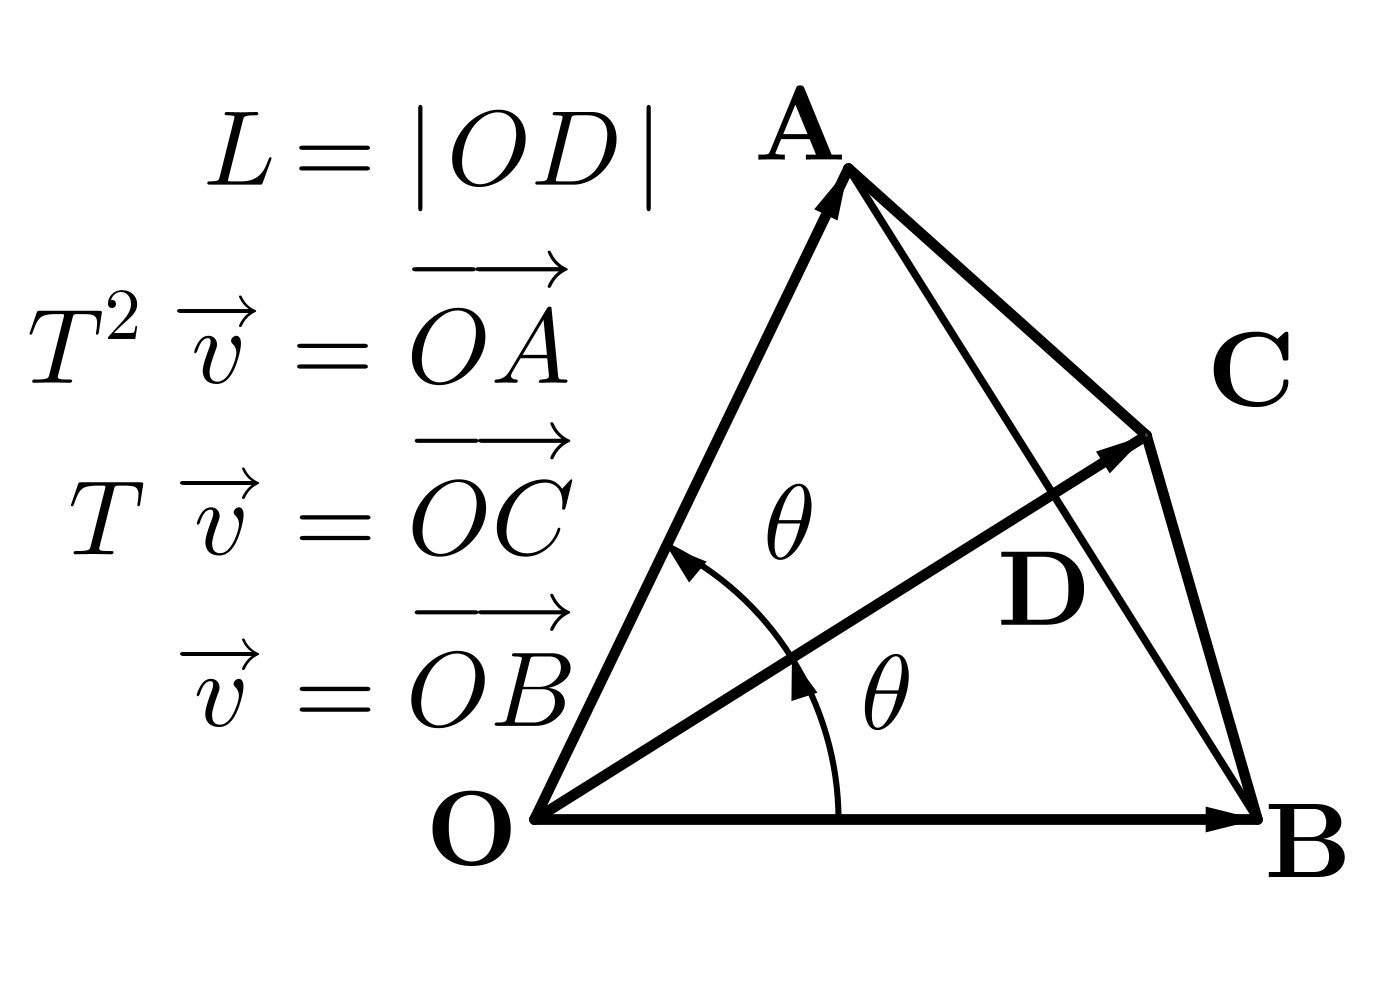
\includegraphics[width=4.4cm,height=3.2cm,scale=0.22]{diagram5BI-1.png}\Blind{\quad}\vspace{-76pt}\parSol{}
Othws, let $\Span{v,Tv}=\Rbb^2.$ Let $L=x^2+y^2,$ where $v=\Par{x,y}.$\parSol{}
Supp $p\Par{z}=z^2+bz+c.$ Let $P=L\cos\theta\Rightarrow L\big/2P=1\big/\Par{2\cos\theta}.$\parSol{}
Then $Tv=\BigPar{L\big/2P}\Par{T^2 v+v}\Rightarrow T=\BigPar{L\big/2P}\Par{T^2+I}.$\parSol{}
Hence $p\Par{T}=T^2-2\cos\theta\, T+I=0.$\PfEnd\vspace{4pt}\parSol{}
\Or Let $\Par{e_1,e_2}$ be the std bss of $\Rbb^2.$ Becs $Te_1=\cos\theta\;e_1+\sin\theta\;e_2,\;T^2e_1=\cos2\theta\;e_1+\sin2\theta\;e_2.$\vspace{0pt}\parSol{}
$ce_1+bTe_1=-T^2 e_1\Longleftrightarrow{}${\small$\begin{pmatrix}1 & \cos\theta\\0 & \sin\theta\end{pmatrix}\begin{pmatrix}c \\ b\end{pmatrix}$}${}={}${\small$\begin{pmatrix}-\cos2\theta\\-\sin2\theta\end{pmatrix}$}. Now $\det=\sin\theta\neq 0,\:c=1,\,b=2\cos\theta.$\PfEnd%\vspace{10pt}\parSol{}
%\Or $\Mt[\BigPar]{T,\Par{e_1,e_2}}={}${\small$\begin{pmatrix}\Blind{-}\cos\theta & \sin\theta\\-\sin\theta & \cos\theta
%\end{pmatrix}$}. By (4E 11), $\Par{z\pm 1}$ or $\Par{z^2-2\cos\theta\,z+1}$ is the min.\PfEnd
\SepLine
		
\Anchor{5BI4e11}\ProblemBnoor{4E 11}{
	\TextA{Supp $V$ is 2\hspace{1pt}-\hspace{1pt}dim, $T\in\Lm{V}$ with the min $p$, and $\Mt[\BigPar]{T,\Par{v,w}}={}${\large$\begin{pmatrix} a &\hspace{-4pt} c\\[-4pt] b &\hspace{-4pt} d\end{pmatrix}.$}\vspace{-8pt}}
	\PrePa\TextA{Show $q\Par{z}=z^2-\Par{a+d}z+\Par{ad-bc}$ is a multi of $p.$}
	\PrePb\TextA{Show if $b=c=0$ and $a=d,$ then $p\Par{z}=z-a;$\;othws $p=q.$}
}(a) $Tv=av+bw\Rightarrow\Par{T-aI}v=bw\Rightarrow\Par{T-dI}\Par{T-aI}v=bTw-bdw=bcv.$\parSol{\Ha}
$Tw=cv+dw\Rightarrow \Par{T-dI}w=cv\Rightarrow\Par{T-aI}\Par{T-dI}w=cTv-acv=bcw.$\vspace{2pt}\parSol{}
(b) {\vspace{-2pt}\FontSmall If $b=c=0$ and $a=d.$ Then $\Mt{T}=a\Mt{I}\Rightarrow T=aI.$ Othws, we show $T\not\in\Span{I},$}\parSol{\Hb}
{\vspace{-2pt}\FontSmall so that $\deg p=\dim V.$ Let (1) $a=d,$ (2) $b=0,$ (3) $c=0.$ Then (1), (2) and (3) cannot be all true.}\parSol{\Hb}
{\vspace{-2pt}\FontSmall(I) Asum (1) is true, with (2) or (3) not true. Then $Tv=av+bw,$ or $Tw=cv+aw\not\in\Span{w}.$}\parSol{\Hb}
{\vspace{-2pt}\FontSmall(II) Asum (2) or (3) are true, with (1) not true. Then $Tv=av+bw,$ or $Tw=cv+dw.$}\PfEnd
\SepLine

\Anchor{5BI4e16}\Anchor{8C18}\ProblemBnoor{8.C.18 \OR 4E 16}{
	\TextA{Define $T\in\Lm{\Fbb^n}:\Par{x_1,\dots,x_n}\mapsto\BigPar{{-a_0\,x_n,\,x_1-a_1\hspace{1pt}x_n,\,\cdots,\,x_{n-1}-a_{n-1}\hspace{1pt}x_n}}.$\vspace{1pt}}
	\TextA{Show the min $p$ of $T$ is $q\Par{z}=a_0+a_1z+\dots+a_{n-1}z^{n-1}+z^n.$}
}Becs $Te_1=e_2,\,T^2e_1=e_3,\cdots,\,T^{n-1}e_1=e_n,\,T^ne_1=T^{n-k}e_{k+1}=Te_n=-\Par{a_0\hspace{1pt}e_1+\dots+a_{n-1}\hspace{1pt}e_n}.$\parSol{}
Let $-T^n=c_0I+c_1T+\dots+c_{n-1}T^{n-1}\Rightarrow$ each $c_k=a_k.$ Becs $n=\dim V.$ No greater deg.\PfEnd
\SepLine

\Anchor{5BI4e17}\ProblemBnoor{{4E 17}}{
	\TextA{Supp $V$ finide, $T\in \Lm{V}$ with the min $p,$ and $\lambda\in\Fbb.$}
	\TextA{Show the min $s$ of $\Par{T-\lambda I}$ is $q\Par{z}=p\Par{z+\lambda}.$}
}Becs $q\Par{T-\lambda I}=p\Par{T}=0\Rightarrow q$ a multi of $s\Rightarrow\deg q=\deg p\geqslant\deg s.$\parSol{}
Define $r\Par{z}=s\Par{z-\lambda}\Rightarrow r\Par{T}=s\Par{T-\lambda I}=0\Rightarrow \deg r=\deg s\geqslant\deg p.$\PfEnd\vspace{2pt}\parSol{}
\Or Becs  $T^k\in\Span{I,T,\dots,T^{k-1}}\Longleftrightarrow\Par{T-\lambda}{^k}\in\Span[\BigBigPar]{I,\Par{T-\lambda I},\dots,\Par{T-\lambda I}{^{k-1}}}.$\PfEnd
\SepLine

\Anchor{5BI4e18}\ProblemBnoor{{4E 18}}{
	\TextA{Supp $V$ is finide, $T\in\Lm{V}$ with the min $p$ of deg $m,$ and $\lambda\neq 0.$}
	\TextA{Show the min $s$ of $\lambda T$ is $q\Par{z}=\lambda^m p\BigPar{{z}\big/{\lambda}}.$}
}Becs $q\Par{\lambda T}=\lambda^m p\Par{T}=0\Rightarrow q$ is multi $s\Rightarrow\deg q=\deg p\geqslant\deg s.$\parSol{}
Define $r\Par{z}=s\Par{\lambda z}\Rightarrow r\Par{T}=s\Par{\lambda T}=0\Rightarrow \deg r=\deg s\geqslant\deg p.$\PfEnd\vspace{2pt}\parSol{}
\Or Becs $\Par{\lambda T}{^k}\in\Span[\BigBigPar]{\lambda I,\lambda T,\dots,\Par{\lambda T}{^{k-1}}}\Longleftrightarrow T^k\in\Span{I,T\dots,T^{k-1}}.$\PfEnd
\SepLine

\Anchor{5BI4e10}\Anchor{5BI4e23}\ProblemBnoor{4E 10, 23}{
	\TextA{Supp $V$ is finide, $T\in\Lm{V},$ with the min $p$ of deg $m.$\vspace{1pt}}
	\TextA{Supp non0 $v\in V.$ Let each $U_k=\Span[\BigPar]{v,Tv,\dots,T^kv}.$\vspace{1pt}}
	\TextA{Prove $\exists\,j\in\Bra{1,\dots,m},\;U_{j-1}=U_n$ for all $n\geqslant j-1.$}
}Supp $j$ is the smallest suth $T^j v=a_0v+a_1 Tv+\dots+a_{j-1}T^{j-1}v\in U_{j-1}\Rightarrow j\leqslant m.$\parSol{}
Then $U_{j-1}$ is invard $T,$ so is each $U_n=\Span{v,Tv,\dots,T^{j-1} v,\dots,T^n v}.$\PfEnd
\SepLine\pagebreak

\Anchor{5BI4e13}\ProblemBnoor{4E 13}{
	\TextA{Supp $V$ finide, $T\in \Lm{V},$ with the min $p\Par{z}=c_0+c_1 z+\dots+c_{m-1}z^{m-1}+z^m.$}
	\TextA{Prove if $q\Par{z}=a_0 +a_1 z+\dots+a_n z^n,$ then $\exists\,!\,r\in\PoF{\deg p-1},\,q\Par{T}=r\Par{T}.$}
}Becs $p\neq 0.$ By the div algo, immed. \Sbra{$r=0$ if $q=p.$}\PfEnd\vspace{2pt}\parSol{}
\Or Becs $T^m=-c_0I-c_1T-\dots-c_{m-1}T^{m-1}.$ For $\deg q<m=\deg p,$ the repres of $q\Par{T}$ is uniq.\parSol{}
Supp $\deg q\geqslant\deg p.$ For each $k\in\Nbb,\exists\,!\,b_{j,k}\in\Fbb,\,T^{m+k}=b_{0,k}I+b_{1,k}T+\dots+b_{m-1,k}T^{m-1}.$\PfEnd
\SepLine

\Anchor{5BI4e14}\ProblemBnoor{4E 14}{
	\TextA{Supp $V$ finide, $T\in\Lm{V},$ with the min $p\Par{z}=a_0 + a_1 z + \dots + a_{m-1} z^{m-1}+z^m,$}
	\TextA{and $a_0\neq 0.$ \,Give a repres of $s,$ the min of $T^{-1}.$\vspace{2pt}}
}Define $q\Par{z}=z^m+{}${\Large$\frac{a_1}{a_0}$}$\,z^{m-1}+\dots+{}${\Large$\frac{a_{m-1}}{a_0}$}$\,z+{}${\Large$\frac{1}{a_0}$}${}\Rightarrow q\Par{T^{-1}}=T^{-m}p\Par{T}=0.$\vspace{2pt}\parSol{}
Becs $\deg s\leqslant\deg q,$ while $\Par{T^{-1}}{^{-1}}=T\Rightarrow\deg q\leqslant\deg s.$\PfEnd\vspace{4pt}\parSol{}
\Or Becs each $T^{-k}\not\in\Span[\BigPar]{I,T^{-1},\dots,T^{-\SmallPar{k-1}}}$ for $k\in\Bra{1,\dots,m-1}.$ Done.\parSol{}
For if not, supp $T^{-k}=b_0 I+b_1 T^{-1}+\dots+b_{k-1}T^{k-1}.$ Note that $T$ inv $\Rightarrow\exists\,b_j\neq 0.$\parSol{}
Now $T^k\Par{T^{-k}}=I=b_0 T^k+b_1 T^{k-1}+\dots+b_{k-1}T\Rightarrow T^j\in\Span{I,T,\dots,T^{k-1}}.$\PfEnd
\SepLine

\Anchor{8C11}\ProblemBnoor{8.C.11}{
	\TextA{Supp $V$ finide and $T\in\Lm{V}$ inv. Prove $\exists\,q\in\PoFi,T^{-1}=q\Par{T}.$}
}By (4E 22), $I=a_1T+\dots+a_mT^m\Rightarrow T^{-1}=a_1I+a_2T+\dots+a_mT^{m-1}.$\PfEnd
\SepLine

\Anchor{5BI4e19}\ProblemBnoor{4E 19}{
	\TextA{Supp $V$ finide, $T\in\Lm{V},$ with the min $p\Par{z}=c_0+c_1z+\dots+c_{m-1}z^{m-1}+z^m.$}
	\TextA{Let $\mE =\Bra{q\Par{T}: q \in \PoFi},$ a subsp of $\Lm{V}.$ Prove $\dim\mE=\deg p.$}
}Becs $T^m=c_0I+c_1T+\dots+c_{m-1}T^{m-1}\Rightarrow U=\Span{I,T,\dots,T^{m-1}}\Rightarrow U$ invard $T$\parSol{}
$\Rightarrow$ each $T^{m+k}=T^k\Par{T^m}\in U\Rightarrow\mE=\Span[\BigPar]{I,T,\dots,T^{\dim\Lm[\SmallPar]{V}-1}}=\Span[\BigPar]{I,T,\dots,T^{m-1}}=U.$\PfEnd\vspace{2pt}\parSol{}
\Or Define $\Phi\in\Lm[\BigPar]{\PoFi,\Lm{V}}$ by $\Phi\Par{q}=q\Par{T}\Rightarrow\range\Phi=\mE.$\parSol{}
Becs $\Phi\Par{q}=q\Par{T}=0\Longleftrightarrow q$ is a multi of the min $p\Longleftrightarrow q\in\Bra{ps:s\in\PoFi}=\null\Phi.$\parSol{}
Now by (4.11), $\dim\PoFi\XSlash\null\Phi=\deg p=m.$ By [3.91](d).\PfEnd
\SepLine

\Anchor{5BI4e29}\ProblemBnoor{{4E 29}}{
	\TextB{Supp $V$ is finide, $\dim V=n\geqslant 2$, and $T\in\Lm{V}.$ Show $T$ has a $2$\hspace{1pt}-\hspace{1pt}dim invarsp.}
}See [9.8] for a graceful proof. \Or Let each $V_{\!k}$ be an arb vecsp of dim $k$ with an arb $T_{\!k}\in\Lm{V_{\!k}}.$\par\quad
Define the stmt $P\Par{k}:$ every optor on a $V_{\!k}$ has invarsp of dim $2.$ (i) $k=2.$ Immed.\par\quad
(ii) $k\geqslant 2.$ Asum $P\Par{k}$ holds. Let $p$ be the min of $T_{\!k+1}=T.$ Note that $V_{\!k+1}$ non0 $\Rightarrow p$ nonC, $\deg p\geqslant 1.$\par\quad
(a) If $p\Par{z}=\Par{z-\lambda}q\Par{z},$ then by (4E 5.A.39), $\exists\,U$ invarspd $T$ of dim $k.$\par\quad\Ha
By asum, the optor $T\mmid_U$ on a $k$\hspace{1pt}-\hspace{1pt}dim vecsp has invarsp of dim $2$, so has $T.$\vspace{2pt}\par\quad
(b) Othws, $T_{\!k+1}$ has no eigvals $\Rightarrow p$ of deg $\geqslant 1$ has no zeros, thus $\Fbb=\Rbb,$ and $\deg p$ is even.\par\quad\Hb
Let $p\Par{z}=\Par{z^2+b_1z+c_1}\cdots\Par{z^2+b_mz+c_m}\Rightarrow\exists\,\Par{T^2+b_jT+c_j}$ not inje\par\quad\Hb
$\Rightarrow\exists\,v\neq 0,\Par{T^2+b_jT+c_j}v=0\Rightarrow T^2v\in\Span{v,Tv},$ invard $T,$ while $\dim\Span{v,Tv}=2.$\PfEnd
\SepLine

\Anchor{5BIN4e5.33}\ProblemBX{\NoteForSmall{[4E 5.33]}}{
	\TextA{Supp $\Fbb=\Rbb,$ $V$ is finide, $T\in\Lm{V},$ and $b^2<4c$ for $b,c\in\Fbb.$}
	\TextB{Prove $\dim\Null\BigPar{T^2+bT+cI}{^j}$ is even for each $j\in\Nbp.$}
}Using induc on $j.$ \,(i) Immed. \,(ii) $j>1.$ Asum it holds for $j-1.$\parSol{}
Replace $V$ with $\Null\Par{T^2+bT+cI}{^{j}}$ and $T$ with $T$ restr to $\Null\Par{T^2+bT+cI}{^{j}}.$\parSol{}
Then $\Par{T^2+bT+cI}{^{j}}=0\Rightarrow z^2+bz+c$ is a multi of the min of $T\Rightarrow$ no eigvecs of $T.$\parSol{}
Let $U$ be invarspd $T$ and has the largest even dim of all such invarsp. If $V=U,$ done. Othws,\parSol{}
for $w\in V\Backslash U\Rightarrow W=\Par{w,Tw}$ invard $T$ of dim $2\Rightarrow U+W$ of dim $\Par{{\dim U+2}}$ invard $T.$\PfEnd
\SepLine

\pagebreak

\ChDecl{Ch5BII}{5.B: II}{\qquad{\small\textbf{注意\,:}\;这一节的题号使用第四版5.C节.}}

\vspace{4pt}

\Anchor{5BII4e2}\ProblemN{2}{
	\TextA{Supp $A$ and $B$ are up-trig \Par{and square} matrices of the same size,}
	\TextA{with $\alpha_1 , \dots , \alpha_n$ on the diag of $A$ and $\beta_1 , \dots , \beta_n$ on the diag of $B$.}
	\PrePa\TextA{Show $A + B$ up-trig with $\alpha_1 + \beta_1 , \dots , \alpha_n + \beta_n$ on the diag.}
	\PrePb\TextA{Show $AB$ up-trig with $\alpha_1 \beta_1 , \dots , \alpha_n \beta_n$ on the diag.}
}(a) By def, immed. \:(b) Becs $A_{j,k}=B_{j,k}=0$ for $j>k.$ By def, for each $p\in\Bra{1,\dots,n},$\parSol{} $\Par{AB}{_{p,p}}=A_{p,1}B_{1,p}+\dots+A_{p,p-1}B_{p-1,p}+A_{p,p}B_{p,p}+A_{p,p+1}B_{p+1,p}+\dots+A_{p,n}B_{n,p}=A_{p,p}B_{p,p}.$\PfEnd
\SepLine

\Anchor{5BII4e3}\ProblemN{3}{
	\TextA{Supp $T$ inv, $B_V=\Par{v_1,\dots,v_n},$ $\Mt{T}=A$ is up-trig,}
	\TextA{with $\lambda_1,\dots,\lambda_n$ on diag. Show $A^{-1}$ is also up-trig, with $\lambda_1^{-1},\dots,\lambda_n^{-1}$ on diag.}
}Becs $\lambda_k$ on diag of $A$ $\Longleftrightarrow\lambda_k$ eigval of $T$ $\Longleftrightarrow\lambda_k^{-1}$ eigval of $T^{-1}$ $\Longleftrightarrow\lambda_k^{-1}$ on diag of $A^{-1}.$\PfEnd\vspace{2pt}\par\quad
\Or Let each $Tv_k=u_k+\lambda_kv_k,$ where $u_k\in\Span{v_1,\dots,v_{k-1}}.$ We use induc on $k.$\par\quad
(i) $k=1.$ $Tv_1=\lambda_1v_1\Rightarrow T^{-1}v_1=\lambda_1^{-1}v_1\in\Span{v_1},$ invard $T^{-1};$ and $\lambda_1^{-1}$ is the 1st ent on diag.\par\quad\Endi
(ii) $k\geqslant 2.$ Asum $\Span{v_1,\dots,v_{k-1}}$ invard $T^{-1}.$\par\quad\Hii
Note that $Tv_k=u_k+\lambda_kv_k\Rightarrow v_k=T^{-1}\Par{c_1v_1+\dots+c_{k-1}v_{k-1}}+\lambda_kT^{-1}v_k.$\par\quad\Hii
Thus $T^{-1}v_k=\lambda_k^{-1}v_k-\lambda_k^{-1}T^{-1}u_k\in\Span{v_1,\dots,v_k},$ invard $T;$ and $\lambda_{k}^{-1}$ is the $k^\text{th}$ ent on diag.\PfEnd
\SepLine

%\Anchor{5BII14}\Anchor{5BII4e4}\ProblemNor{4}{3E 5.B.14}{
%	\TextA{Give an inv $T$ and a $B_V$ suth each $\Mt{T}{_{k,k}}=0.$}
%}Define $T\in\Lm{\Rbb^2}:\Par{x,y}\mapsto\Par{y,x}.$
%\SepLine
%
%\Anchor{5BII15}\Anchor{5BII4e5}\ProblemNor{5}{3E 5.B.15}{
%	\TextA{Give a non-inv $T$ and a $B_V$ suth each $\Mt{T}{_{k,k}}\neq 0.$}
%}Define $T\in\Lm{\Fbb^2}:\Par{z,w}\mapsto\Par{z+w,z+w}.$
%\SepLine

%\Anchor{5BII20}\Anchor{5BII4e6}\ProblemNor[]{6}{3E 5.B.20}{
%	\TextA{Supp $\Fbb=\Cbb,$ $V$ is finide, $T\in\Lm{V},$ and $k\in\Bra{1,\dots,\dim V}.$}
%	\TextA{Prove $V$ has a $k$\hspace{1pt}-\hspace{1pt}dim invarspd $T.$\hfill\FontNorm\tgnr By [5.27] and [5.26], immed.\vspace{-3pt}}
%}\SepLine

\Anchor{5BII4e8}\ProblemN{8}{
	\TextA{Supp $V$ is finide, and $v\in V$ is non0 suth $q\Par{T}v=0,$ where $q\Par{z}=z^2+2z+2.$}
	\PrePa\TextA{Supp $\Fbb=\Rbb.$ Prove $\nexists\,B_V$ suth $\Mt{T}$ up-trig.}
	\PrePb\TextA{Supp $\Fbb=\Cbb,$ and $\exists\,B_V$ suth $A=\Mt{T}$ up-trig. Prove $-1+\i$ or $-1-\i$ on diag.}
}Define $p_v$ as (4E 3.C.7). Note that $\deg p_v\geqslant 1$ becs $v\neq 0.$ 又 $q\Par{T\mmid_{\nullp p_v\SmallPar{v}}}=0.$\parSol{}
Now $q$ of deg $2$ is a multi of the min of $T\mmid_{\nullp p_v\SmallPar{v}},$ which is $p_v,$ of which the min of $T$ is a multi.\parSol{}
(a) Note that $q$ has no $1$\hspace{1pt}-\hspace{1pt}deg factors $\Rightarrow\deg p_v\geqslant 2.$ By [4E 5.44].\parSol{}
(b) $q\Par{z}=\Par{z+1+\i}\Par{z+1-\i}\Rightarrow -1-\i$ or $-1+\i$ zero of $p_v\Rightarrow$ is eigval $\Rightarrow$ on diag.\PfEnd
\SepLine

\Anchor{5BII4e9}\ProblemN{9}{
	\TextA{Supp $B\in\Cbb^{n,n}.$ Prove $\exists$ inv $A\in\Cbb^{n,n}$ suth $A^{-1} BA$ is up-trig.}
}Define $T\in\Cbb^n$ with $B=\Mt[\BigPar]{T,\Par{e_1,\dots,e_n}}.$ Let $C=\Mt[\BigPar]{T,\Par{f_1,\dots,f_n}}$ be up-trig.\parSol{}
Let $A=\Mt[\BigPar]{I,\,f\rightarrow e}.$ Then $C=A^{-1}BA.$\PfEnd
\SepLine

\Anchor{5BII4e10}\ProblemN{10}{
	\TextA{Supp $B_V=\Par{v_1,\dots,v_n},A=\Mt{T,B_V}.$ Show the following are equiv\hspace{1pt}$:$}
	\PrePa\TextA{$A$ is low-trig. \:{\tgnr\large(b)} Each $Tv_k\in\Span{v_k,\dots,v_n}.$ \:{\tgnr\large(c)} Each $\Span{v_k,\dots,v_n}$ invard $T.$}
}By def, (a) and (b) are equiv, and (c) $\Rightarrow$ (b). Now supp (b) holds. For any $k\in\Bra{1,\dots,n}.$\parSol{}
$Tv_k\in\Span{v_k,\dots,v_n},\,Tv_{k+1}\in\Span{v_{k+1},\dots,v_n},\cdots,\,Tv_{n}\in\Span{v_n}.$ Thus (c) holds.\PfEnd
\SepLine

\Anchor{5BIIT1}\BulletPointX\TipsN{1}\;\;Supp $B_V=\Par{v_1,\dots,v_n},B_{V\apostrophe}=\Par{\varphi_1,\dots,\varphi_n},T\in\Lm{V},A=\Mt{T,B_V}.$\TextB{}
\IndentTipsN{1}(a) $A$ up-trig $\Longleftrightarrow T=\sum_{k=1}^n\sum_{j=1}^kA_{j,k}E_{k,j}\Longleftrightarrow T\apostrophe=\sum_{k=1}^n\sum_{j=1}^kA^t_{k,j}\reflectbox{\textit{E}}{_{j,k}}\Longleftrightarrow A^t$ low-trig.\TextB{}
\IndentTipsN{1}(b) $A$ low-trig $\Longleftrightarrow T=\sum_{k=1}^n\sum_{j=1}^kA_{k,j}E_{j,k}\Longleftrightarrow T\apostrophe=\sum_{k=1}^n\sum_{j=1}^kA^t_{j,k}\reflectbox{\textit{E}}{_{k,j}}\Longleftrightarrow A^t$ up-trig.\par
\SepLine

\Anchor{5BIIT2}\ProblemBX{\TipsN{2}}{
	\TextA{Supp $\Par{\alpha_1,\dots,\alpha_n},\Par{\beta_1,\dots,\beta_n}$ are bses of $V,$ with each $\alpha_k=\beta_{n-k+1}.$}
	\TextA{Prove $\Mt{T,\alpha\rightarrow\alpha}$ up-trig $\Longleftrightarrow\Mt{T,\beta\rightarrow\beta}$ low-trig.}
}For each $k\in\Bra{1,\dots,n},\:T\beta_{n-k+1}=T\alpha_k\in\Span{\alpha_1,\dots,\alpha_k}=\Span{\beta_n,\dots,\beta_{n-k+1}}.$\PfEnd\vspace{2pt}
\Anchor{5BII4e11}\Anchor{5BII4e14}\ACoro (a) Supp $\Fbb=\Cbb.$ Then $\exists\,B_V$ suth $\Mt{T,B_V}$ low-trig. \;(b) $T$ up-trig $\Longleftrightarrow T\apostrophe$ up-trig.
\SepLine

\Anchor{5BII4e12}\Anchor{5BII4e13}\ProblemN{12, 13}{
	\TextA{Supp $V$ finide, $T\in\Lm{V}.$ Prove $T\mmid_U,T\XSlash U$ up-trig for some $U$ invarsp $\Longleftrightarrow T$ up-trig.}
}Supp $B_U=\Par{u_1,\dots,u_p},B_{V\XSlash U}=\Par{w_1+U,\dots,w_q+U}$ suth $\Mt{T\mmid_U},\Mt{T\XSlash U}$ up-trig.\parSol{}
Then each $Tu_k\in\Span{u_1,\dots,u_k}$ and each $Tw_j+U\in\Span{w_1+U,\dots,w_j+U}.$\parSol{}
By (3.E.13), $B_V=\Par{u_1,\dots,u_p,w_1,\dots,w_q}.$ Now each $Tw_j\in\Span{u_1,\dots,u_p,w_1,\dots,w_j}.$\PfEnd\vspace{2pt}\parSol{}
\Or By (4E 5.B.25)(b) and [4E 5.44], immed.\quad Convly, by [4E 5.44], immed.\PfEnd
\SepLine
\ChEnd

\ChDecl{Ch5C}{5.C \& [4E] 5.D}{\qquad{\small\textbf{注意\,:}\;这一节的题号主要使用第四版5.D节.}}

\vspace{6pt}

\Anchor{5C4e15}\ProblemN[]{15}{
	Supp $\Fbb=\Cbb,$ $V$ is finide, $T\in\Lm{V}$ with the min $p.$ Then using Exe (4.6),\TextA{}
	$T$ diag $\Longleftrightarrow\nexists\,\Par{z-\lambda}{^2}$ in $p\Longleftrightarrow p,p\apostrophe$ have no common zeros $\Longleftrightarrow\gcd\Par{p,p\apostrophe}=1.$\vspace{-4pt}\TextA{}
}\SepLine

\Anchor{5C1}\Anchor{5C4e3}\ProblemN{3}{
	\TextA{Supp $T\in\Lm{V}$ is diag. Prove $V=\null T\oplus\range T.$}
}Let $U=E\Par{\lambda_1,T}\oplus\cdots\oplus E\Par{\lambda_m,T},$ where each $\lambda_k\neq 0$ and $B_{E\SmallPar{\lambda_k,T}}=\Par{v_{1,k},\dots,v_{M_k,k}}.$\parSol{}
Becs $\null T=E\Par{0,T}\Rightarrow$ whether $0$ is eigval or not, $V=U\oplus\null T.$ Now we show $U=\range T.$\parSol{}
By (3.B.12), $\range T=\Bra{Tu:u\in U}=\BigBra{\sum_{k=1}^m\lambda_k\Par{a_{1,k}v_{1,k}+\dots+a_{M_k,k}v_{M_k,k}}:a_{j,k}\in\Fbb}=U.$\PfEnd\vspace{2pt}
\AExa Convly not true. Define the inv $T\in\Lm{\Rbb^2}:\Par{x,y}\mapsto\Par{{-y,x}}.$ No eigvals.
\SepLine

\Anchor{5CL1}\ProblemN{L1}{
	\TextA{Supp $T\in\Lm{V},\alpha,\beta\in\Fbb$ and $\alpha\neq\beta.$ Prove $\Null\Par{T-\alpha I}\subseteq\Range\Par{T-\beta I}.$}
}$\forall v\in\Null\Par{T-\alpha I},Tv=\alpha v\Rightarrow\Par{T-\beta I}\Sbra{v\Big/\Par{\alpha-\beta}}=v\in\Range\Par{T-\beta I}.$\PfEnd
\SepLine

\Anchor{5C5}\Anchor{5C4e5}\ProblemN{5}{
	\TextA{Supp $\Fbb=\Cbb,$ $V$ is finide, and $T\in\Lm{V}.$}
	\TextA{Supp $V=\Null\Par{T-\lambda I}\oplus\Range\Par{T-\lambda I}$ for all $\lambda\in\Cbb.$ Prove $T$ is diag.}
}(i) $\dim V=1.$ Immed. (ii) $\dim V>1.$ Asum it holds for vecsps of smaller dim.\parSol{}
$\exists$ eigval $\lambda_0\Rightarrow U=\Range\Par{T-\lambda_0I}$ invard $T\Rightarrow U=\Null\Par{T\mmid_U-\lambda I}\oplus\Range\Par{T\mmid_U-\lambda I}.$\parSol{}
While $V=E\Par{\lambda_0,T}\oplus U\Rightarrow\dim U<\dim V.$ By asum, $T\mmid_U$ is diag wrto $B_U$ of eigvecs.\PfEnd\vspace{4pt}\par\quad
\Or Supp $T$ not diag. We show $\exists\,\lambda\in\Cbb,\,\Null\Par{T-\lambda I}\cap\Range\Par{T-\lambda I}\neq\zeroSubs.$\par\quad
Let the min of $T$ be $p\Par{z}=\Par{z-\lambda_1}{^{\alpha_1}}\cdots\Par{z-\lambda_m}{^{\alpha_m}},$ where each $\alpha_k\geqslant 1$ and $\exists\,\alpha_j>1.$\par\quad
Let $q\Par{z}\Par{z-\lambda_j}=p\Par{z}\Rightarrow 0=p\Par{T}=\Par{T-\lambda_j}q\Par{T}\Rightarrow\rangep q\Par{T}\subseteq\Null\Par{T-\lambda_jI}.$\par\quad
Let $q\Par{z}=\Par{z-\lambda_j}s\Par{z}\Rightarrow\rangep q\Par{T}\subseteq\Range\Par{T-\lambda_jI}.$ \,Note that $q\Par{T}\neq0.$\PfEnd\vspace{6pt}\quad
\Or Let $\lambda_1,\dots,\lambda_m$ be disti eigvals. Now $V=\Null\Par{T-\lambda_kI}\oplus\Range\Par{T-\lambda_kI}$ for each $\lambda_k.$\par\quad
%By (L1) and \Sbra{1.C \TIPSN{3}}, $\Range\Par{T-\lambda_1I}=\Null\Par{T-\lambda_2I}\oplus\Sbra{\Range\Par{T-\lambda_2I}\cap\Range\Par{T-\lambda_1I}}.$\par\quad
Asum $V=\Sbra{\bigoplus_{i=1}^j\Null\Par{T-\lambda_jI}}\oplus\Sbra{\bigcap_{i=1}^j\Range\Par{T-\lambda_jI}}$ for $j\in\Bra{1,\dots,m-1}.$\par\quad
Becs $\bigcap_{i=1}^j\Range\Par{T-\lambda_iI}\supseteq\Null\Par{T-\lambda_{j+1}I}.$ By (L1) and \Sbra{1.C \TIPSN{3}},\par\quad
$\bigcap_{i=1}^j\Range\Par{T-\lambda_iI}=\Null\Par{T-\lambda_{j+1}I}\oplus\Sbra{\bigcap_{i=1}^j\Range\Par{T-\lambda_jI}\cap\Range\Par{T-\lambda_{j+1}I}}.$\par\quad
By induc, $V=\Sbra{\Null\Par{T-\lambda_1I}\oplus\cdots\oplus\Null\Par{T-\lambda_mI}}\oplus\Sbra{\Range\Par{T-\lambda_1I}\cap\cdots\cap\Range\Par{T-\lambda_mI}}.$\par\quad
Asum $U=\bigcap_{k=1}^m\Range\Par{T-\lambda_kI}\neq\zeroSubs.$ Becs $U$ invard $T.$ Thus $\exists\,\mu=\lambda_j$ eigval of $T\mmid_U.$ Ctradic.\PfEnd
\SepLine

%\Anchor{5C7}\Anchor{5C4e2}\ProblemN{2}{
%	\TextA{Supp $T\in\Lm{V},A=\Mt{T,B_V}$ is diag. Prove $A$ has $\dim E\Par{\lambda,T}$ $\lambda$'s on diag.}
%}Given eigvecs $B_V=\Par{v_1,\dots,v_n}.$ Becs $T$ diag. Each $Tv_k=\lambda_jv_k.$ Forming $B_{E\SmallPar{\lambda_j,T}}.$ Immed.\PfEnd%%\vspace{2pt}\parSol{}
%%\Or Let $\lambda_1,\dots,\lambda_m$ be the disti non0 eigvals. Supp $d_0$ eigvecs of $B_V$ corres eigval $0\Rightarrow\dim E\Par{0,T}=d_0.$
%\SepLine

\Anchor{5C4e13}\ProblemN{13}{
	\TextA{Supp $A,B\in\Fbb^{n,n}$ and $A$ is diag with {\tgsc dist} ents on diag. Prove $AB=BA\Longleftrightarrow B$ is diag.}
}\NOTICE that for any diag $C,$ each $C_{j,k}=0$ for $j\neq k.$\parSol{}
Becs (I) $A_{j,j}B_{j,k}=A_{j,1}B_{1,k}+\dots+\Sbra{A_{j,j}B_{j,k}}+\dots+A_{j,n}B_{n,k}=\Par{AB}{_{j,k}}.$\parSol{}
And (II) $B_{j,k}A_{k,k}=B_{j,1}A_{1,k}+\dots+\Sbra{B_{j,k}A_{k,k}}+\dots+B_{j,n}A_{n,k}=\Par{BA}{_{j,k}}.$\parSol{}
Supp $B$ diag. If $j=k,$ then $\Par{BA}{_{j,k}}=\Par{AB}{_{j,k}},$ othws true as well.\parSol{}
Supp $AB=BA\Rightarrow A_{j,j}B_{j,k}=A_{k,k}B_{j,k}.$ Asum $B_{j,k}\neq0$ with $j\neq k.$ Then $A_{j,j}=A_{k,k},$ ctradic.\PfEnd
\SepLine

\Anchor{5C4e14}\ProblemN{14}{
	\TextA{Supp $\Fbb=\Cbb,$ $k\in\Nbp,$ and $T\in\Lm{V}$ is inv. Prove $T^k$ diag $\Rightarrow T$ diag.}
}Let the min of $T^k$ be $p\Par{z}=\Par{z-\lambda_1}\cdots\Par{z-\lambda_m}\Rightarrow$ each $\lambda_k$ non0 and disti.\parSol{}
Becs any non0 $\lambda\in\Cbb$ has $k$ disti $k^{\text{th}}$ roots. Let $\Bra{\mu_{1,j},\dots,\mu_{k,j}}$ be the roots of $z^k=\lambda_j.$\parSol{}
For $x,y\in\Bra{1,\dots,n},\:x\neq y\Longleftrightarrow \mu_{p,x}^k=\lambda_x\neq\lambda_y=\mu_{q,y}^k$ for each $p,q\in\Bra{1,\dots,k}\Rightarrow\mu_{p,x}\neq\mu_{q,y}.$\parSol{}
Thus all $\mu$'s are dist. Let $s\Par{z}=\Par{z^k-\lambda_1}\cdots\Par{z^k-\lambda_m}=\prod_{j=1}^m\prod_{i=1}^k\Par{z-\mu_{i,j}}\Rightarrow s\Par{T}=0.$\PfEnd\vspace{3pt}
\AExa Not true if $\Fbb=\Rbb.$ Define $T\in\Lm{\Rbb^2}:\Par{x,y}\mapsto\Par{{-y,x}}.$ No eigvals.
\SepLine

\Anchor{5C'1}\ProblemB{
	\TextB{Supp $\Fbb=\Cbb,n\in\Nbp,p\in\PoFi$. Prove $T\in\Lm{V}$ is diag $\Longleftrightarrow\nullp p\Par{T}=\Null\Sbra{p\Par{T}}{^n}.$}
}(a) Supp $T$ diag. Let $p\Par{z}=\Par{z-\alpha_1}\cdots\Par{z-\alpha_m}.$ We show each $\Null\Par{T-\alpha_kI}{^n}=\Null\Par{T-\alpha_kI}.$\parSol{\Ha}
Done if $T-\alpha_kI=S$ inje. Supp $S$ not inje. \NOTICE that $\null S\mmid_{\range S}=\null S\cap\range S=\zeroSubs.$\parSol{\Ha}
By (3.B.22), $\dim\null S^2=\dim\null S\Rightarrow\null S^2=\null S.$ Asum $\null S^j=\null S$ for $j\geqslant 2.$\parSol{\Ha}
Becs $\dim\Null\Par{S^jS}=\Dim\Par{\null S^j\cap\range S}+\dim\null S.$ By induc.\vspace{3pt}\parSol{}
(b) Supp $\Null\Par{T-\lambda I}=\Null\Par{T-\lambda I}{^n}$ for all $\lambda\in\Cbb.$ Let $\lambda_1,\dots,\lambda_m$ be disti eigvals of $T.$\parSol{\Hb}
Define $p\Par{z}=\Par{z-\lambda_1}\cdots\Par{z-\lambda_m}.$ Then $\Sbra{p\Par{T}}{^{\dim V}}=0\Rightarrow p\Par{T}=0\Rightarrow p$ is the min.\PfEnd
\SepLine

%\Anchor{5C4e17}\ProblemN{17}{
%	\TextA{Supp $V$ is finide. Prove $\Lm{V}$ has a bss consisting of diag optors.}
%}Let $B_V=\Par{v_1,\dots,v_n}.$ Define each $E_{j,k}\in\Lm{V}:v_x\mapsto\delta_{j,x}v_k\Rightarrow$ [5.41](c) true.\PfEnd
%\SepLine

\Anchor{5C4e18}\ProblemN{18}{
	\TextA{Supp $T\in\Lm{V}$ is diag. Prove $T\XSlash U\in\Lm{V\XSlash U}$ is diag for any $U$ invarspd $T.$}
}By \Sbra{5.A \TIPSN{2}}, $\exists\,B_U=\Par{v_1,\dots,v_m}$ consists of eigvecs of $T.$\parSol{}
Extend to eigvecs $B_V=\Par{v_1,\dots,v_m,w_1,\dots,w_p}\Rightarrow B_{V\XSlash U}=\Par{w_1+U,\dots,w_p+U}.$\parSol{}
Becs for each $w_k,\:\exists$ eigval $\lambda$ of $T,\:Tw_k=\lambda w_k\Rightarrow\BigPar{T\XSlash U}\Par{w_k+U}=\lambda w_k+U.$\PfEnd\vspace{2pt}\parSol{}
\Or Becs the min of $T$ is multi of that of $T\XSlash U.$ By [4E 5.62].\PfEnd\vspace{2pt}
\Anchor{5C4e19}\AExa Define $T\in\Lm{\Fbb^2}:\Par{x,y}\mapsto\Par{y,0}.$ Then $0$ is the only eigval with $E\Par{0,T}=\Span{e_1}=U.$\parExa
Then $T\mmid_U=0,T\XSlash U=0.$ \;Now $T\mmid_U,T\XSlash U$ diag while $T$ not diag.\PfEnd
\SepLine

%\Anchor{5C4e20}\ProblemN{20}{
%	\TextA{Supp $V$ is finide, $T\in\Lm{V}.$ Prove $T$ diag $\Longleftrightarrow T\apostrophe$ diag.\hfill\tgnr\FontNorm By (4E 5.B.28), immed.}
%}By \Sbra{5.B(II) \TIPSN{1}}. Note that $S$ low-trig and up-trig $\Longleftrightarrow S$ diag.\PfEnd
%\SepLine

\Anchor{5C4e22}\ProblemN{22}{
	\TextA{Supp $V$ finide, $T\in\Lm{V},$ $A=\Mt{T,B_V}\in\Fbb^{n,n}.$}
	\TextA{Prove if each $\aXMid{A_{j,j}}>\sum_{k=1}^n\aXMid{A_{j,k}}-A_{j,j},$ then $T$ is inv.\vspace{1pt}}
}If $T$ inv $\Rightarrow 0$ is eigval, then $0$ is in G disk for some $j$, now $\aXMid{0-A_{j,j}}\leqslant\sum_{k=1}^n\aXMid{A_{j,k}}-A_{j,j},$ ctradic.\PfEnd\vspace{2pt}
\AComm If each $\aXMid{A_{k,k}}>\sum_{j=1}^n\aXMid{A_{j,k}}-A_{k,k},$ then becs [5.67] still holds by Exe (4E 23), $T$ is inv.
\SepLine

\Anchor{5C4e23}\ProblemN{23}{
	\TextA{Redefine G disks suth the radius of the $k^\text{th}$ disk is the sum of the absolute vals}
	\TextA{of the ents in {\tgsc col} $k$, excluding the diag ent. Show [4E 5.67] still holds.}
}Supp $T\in\Lm{V},B_V=\Par{v_1,\dots,v_n},A=\Mt{T,B_V}.$ Simlr to [5.67]. Let $B_{V\apostrophe}=\Par{\varphi_1,\dots,\varphi_n}.$\vspace{1.5pt}\parSol{}
Supp $T\apostrophe\Par{\psi}=\lambda\psi$ with $\psi=c_1\varphi_1+\dots+c_n\varphi_n\neq0\Rightarrow\lambda\psi=\sum_{j=1}^n\BigBigPar{{\sum_{k=1}^nA^t_{j,k}c_kv_j}}=\sum_{j=1}^nc_j\lambda v_j.$\vspace{3pt}\parSol{}
Let $\aMid{c_j}=\max\!\Bra{\aMid{c_1},\dots,\aMid{c_n}}.$ Now $\lambda c_j=\sum_{k=1}^nA^t_{j,k}c_k\Rightarrow\aXMid{\lambda-A^t_{j,j}}\leqslant\sum_{j\neq k=1}^n\aXMid{A_{k,j}}.$\PfEnd\vspace{6pt}\parSol{}
\Or Becs $\lambda$ is eigval of $T\Longleftrightarrow$ of $T\apostrophe.$ For $A^t=\Mt{T\apostrophe,B_{V\apostrophe}},$ by [5.67],\vspace{1pt}\parSol{}
$\lambda\in\BigBra{z\in\Fbb:\aXMid{z-A_{j,j}}\leqslant\sum_{j\neq k=1}^n\aXMid{A^t_{j,k}}=\sum_{j\neq k=1}^n\aXMid{A_{k,j}}}$ for some $j\in\Bra{1,\dots,n}.$\PfEnd
\SepLine
\ChEnd\pagebreak

\ChDecl{Ch5E}{5.E [4E]}{}

\vspace{4pt}

\Anchor{5E8}\ProblemN{8}{
	\TextA{Find a bss of $\PoFx{m}{\Rbb^2}$ suth $D_x,D_y$ up-trig in [5.72].}
}Let $B=\Par{1,x,y,x^2,xy,y^2,\cdots,\cdots,x^m,x^{m-1}y,\cdots,xy^{m-1},y^m}$ in $\PoFx{m}{\Rbb^2}.$\parSol{}
Supp a liney combina of $B$ is $0;$ \;$\sum_{j=0}^m\sum_{k=0}^{m-j}a_{j,k}x^jy^k=0.$\parSol{}
Let $x=0\Rightarrow$ each $a_{0,k}=0,$ and $y=0\Rightarrow$ each $a_{k,0}=0.$ Now $\sum_{j=1}^{m-1}\sum_{k=1}^{m-1-j}a_{j,k}x^jy^k=0.$\parSol{}
Take $\BigPar{\Par{x_1,y_1},\cdots,\Par{x_q,y_q}}$ \Sbra{where $q=1+\dots+m$} suth all $\sum_{j=1}^{m-1}\sum_{k=1}^{m-1-j}x_s^jy_t^k\,a_{j,k}=0$\parSol{}
form a system of $q$ equations having uniq solus $\Par{0,\dots,0}.$ Thus $B$ is liney indep.\parSol{}
Apply $D_x$ to each vec in $B\Rightarrow B_x=\BigPar{0,1,0,2x,y,0,\cdots,\cdots,mx^{m-1},\Par{m-1}x^{m-2}y,\cdots,y^{m-1},0}.$\parSol{}
Apply $D_y$ to each vec in $B\Rightarrow B_y=\BigPar{0,0,1,0,x,2y,\cdots,\cdots,0,x^{m-1},\cdots,\Par{m-1}xy^{m-2},my^{m-1}}.$\PfEnd
\SepLine

\Anchor{5E6}\ProblemN{6}{
	\TextA{Supp $\Fbb=\Cbb,$ $V$ is finide, and $S, T\in\Lm{V}$ commu.}
	\TextA{Prove $\exists\,\alpha,\lambda\in\Cbb$ suth $\Range\Par{S -\alpha I} + \Range\Par{T -\lambda I}\neq V$.}
}Supp $A,C\in\Fbb^{n,n}$ are up-trig matrices of $S,T$ wrto a $B_V=\Par{v_1,\dots,v_n}$ suth $A,C$ commu.\parSol{}
Let $\alpha=A_{n,n},\,\lambda=C_{n,n}.$ Then $\Range\Par{S-\alpha I},\Range\Par{T-\lambda I}\subseteq\Span{v_1,\dots,v_{n-1}}.$\PfEnd
\SepLine

\Anchor{5E7}\ProblemN{7}{
	\TextA{Supp $\Fbb=\Cbb,$ and $S,T\in\Lm{V}$ commu, $S$ diag. Prove $\exists\,B_V$ suth $S$ diag and $T$ up-trig.}
}Let $\lambda_1,\dots,\lambda_m$ be disti eigvals of $S\Rightarrow V=E\Par{\lambda_1,S}\oplus\cdots\oplus E\Par{\lambda_m,S}.$\parSol{}
Becs each $E_k=E\Par{\lambda_k,S}$ invard $T.$ Let each $T\mmid_{E_k}$ be up-trig with $B_{E_k}=\Par{v_{1,k},\dots,v_{M_k,k}}.$\parSol{}
Then $S$ diag while $T$ up-trig with the same $B_V=\Par{v_{1,1},\dots,v_{M_n,n}}.$\PfEnd\vspace{3pt}\parSol{}
\Or Using induc on $n=\dim V.$ (i) $n=1.$ Immed. \:(ii) $n>1.$ Asum it holds for smaller $V.$\parSol{}
$\exists$ eigval $\lambda$ of $S,\;U=\Null\Par{S-\lambda I},W=\Range\Par{S-\lambda I}\Rightarrow V=\Null\Par{S-\lambda I}\oplus\Range\Par{S-\lambda I}.$\parSol{}
Apply the asum to $T\mmid_U,S\mmid_U$ and $T\mmid_W,S\mmid_W,$ then put $B_U,B_W$ together.\PfEnd
\SepLine

\Anchor{5E2}\ProblemN{2}{
	\TextA{Supp $\mE\subseteq\Lm{V}$ and every elem of $\mE$ diag.}
	\TextA{Prove each pair of elems of $\mE$ commu $\Rightarrow\exists\,B_V$ suth all elem of $\mE$ diag.}
}Let $\dim V=n\Rightarrow\dim\Lm{V}=n^2.$\par\quad
$\exists\,\Bra{T_1,\dots,T_m}\subseteq\mE$ with each elem of $\mE$ in $\Span{T_1,\dots,T_m}$ and $m\leqslant n^2$\par\quad
For each $T_k,$ becs $V=\bigoplus_{\lambda_k\!\!}E\Par{\lambda_k,T_k}$ and $E\Par{\lambda_k,T_k}$ non0 for finily many $\lambda_k\in\Fbb.$\vspace{2pt}\par\quad
Becs $U_{k}=E\Par{\lambda_1,T_1}\cap\cdots\cap E\Par{\lambda_{k},T_{k}}=E\Par{\lambda_k,T_k\mmid_{U_{k-1}}}=\bigoplus_{\lambda_{k+1}\!\!}E\Par{\lambda_{k+1},T_{k+1}\mmid_{U_{k}}}=\bigoplus_{\lambda_{k+1}\!\!}U_{k+1}$.\vspace{2pt}\par\quad
Hence $V=\bigoplus_{\lambda_1\!\!}E\Par{\lambda_1,T_1}=\bigoplus_{\lambda_1,\dots,\lambda_m\!\!}\Sbra{E\Par{\lambda_1,T_1}\cap\cdots\cap E\Par{\lambda_m,T_m}}.$ Take bss of each summand.\vspace{2pt}\par\quad
Then we form $B_V.$ For any $T\in\mE,$ $\Mt{T,B_V}=c_1\Mt{T_1,B_V}+\dots+c_m\Mt{T_m,B_V}.$\PfEnd
\SepLine

\Anchor{5E9}\ProblemN{9}{
	\TextA{Supp $\Fbb=\Cbb,$ $V$ finide and non0. Supp $\mE\subseteq\Lm{V}$ is suth all $S,T\in\mE$ commu.}
	\PrePa\TextA{Prove $\exists$ eigvec $v\in V$ of all elem of $\mE.$ \,{\tgnr\large(b)} $\exists\,B_V$ suth all elem of $\mE$ has up-trig matrix.}
}Simlr to Exe (2). $\exists\,\Bra{T_1,\dots,T_m}\subseteq\mE.$ Let $U_0=V,U_k=E\Par{\lambda_1,T_1}\cap\cdots\cap E\Par{\lambda_k,T_k}.$\parSol{}
(a) Let $\lambda_1,\dots,\lambda_m$ be eigvals of $T_1,\dots,T_m$ respectly with each $\lambda_k$ eigval of $T_k\mmid_{U_k}\Rightarrow U_k\neq 0$\parSol{\Ha}
Now for non0 $v\in U_m,\:\forall T=c_1T_1+\dots+c_mT_m\in\mE,Tv=\Par{c_1\lambda_1+\dots+c_m\lambda_m}v.$\vspace{3pt}\parSol{}
(b) Using induc on $\dim V.$ (i) Immed. \,(ii) $\dim V>1.$ Asum it holds for smaller $V.$\parSol{\Hb}
Let $v_1$ be a common eigvec of all $T_k.$ Let $W\oplus\Span{v_1}=V,P:av_1+w\mapsto w.$\parSol{\Hb}
Simlr in [4E 5.80], each pair of $\Bra{\hat{T}_{1},\dots,\hat{T}_m}$ commu. By asum, $\exists\,B_W\Rightarrow\exists\,B_V.$\parSol{\Hb}
Now each $\Mt{T_k,B_V}$ up-trig $\Rightarrow\forall T\in\mE,\Mt{T}=c_1\Mt{T_1}+\dots+c_m\Mt{T_m},$ wrto $B_V.$\PfEnd
\SepLine\ChEnd
\pagebreak

\ChDecl{Ch8}{8}{\quad{\ANote {\FontSmall $V$ denotes a finide non0 vecsp over $\Fbb.$ An Exe marked by $\blacksquare$ is true if infinide or partially finide.}}}

\vspace{4pt}

\Anchor{Ch8A}

\Anchor{8A3}\ProblemN{A.3}{
	\TextA{Supp $T\in\Lm{V}$ inv. Prove $G\Par{\lambda,T}=G\Par{\lambda^{-1},T^{-1}}$ for any non0 $\lambda\in\Fbb.$\PfEndB}
}$\Par{T-\lambda I}{^j}v=0=\sum_{i=0}^j\mathC_j^i\Par{-\lambda}{^{j-i}}T^iv.$ Apply $\Par{-\lambda}{^{-j}}T^{-j}$ to both sides. $\Par{T^{-1}-\lambda^{-1}}{^j}v=0.$\PfEnd\vspace{2pt}\parSol{}
\Or We use induc on $j$ to show each $\Null\Par{T-\lambda I}{^j}=\Null\Par{T^{-1}-\lambda^{-1}}{^j}.$ \,(i) Immed. (ii) $j>1.$\parSol{}
Asum true for $\Par{j-1}.$ $\forall v\in\Null\Par{T-\lambda I}{^j},\Par{T-\lambda I}v\in\Null\Par{T-\lambda I}{^{j-1}}=\Null\Par{T^{-1}-\lambda^{-1}I}{^{j-1}}.$\parSol{}
Thus $0=\Par{T^{-1}-\lambda^{-1}I}{^{j-1}}\Par{T-\lambda I}v=\uline{\Par{T-\lambda I}}\Par{T^{-1}-\lambda^{-1}I}{^{j-1}}v.$ \;By (i) and rev the roles.\PfEnd
\SepLine

\Anchor{8A5}\ProblemN{A.5}{
	\TextA{Supp $T\in\Lm{V},$ $T^{n-1}v\neq 0,\;T^nv=0.$ \,Prove $\BigPar{v,Tv,\dots,T^{n-1}v}$ is liney indep.}
}$a_0v+a_1Tv+\dots+a_{n-1}T^{n-1}v=0\Rightarrow a_0T^{n-1}v=0\Rightarrow a_0=0.$ \,Simlr for $a_1,\dots,a_{n-1}.$\PfEndB
\SepLine

\Anchor{8A4e24}\Anchor{8N8.19}\ProblemBX[]{\NoteForSmall{[8.19] \OR [4E 8.18]}}{
	If the min of $T$ is $z^m.$ Then $\exists\,v$ suth $T^{m-1}v\neq0.$ If $m=\dim V.$\TextB{}
	Now $B_V=\Par{T^{m-1}v,\dots,Tv,v}.$ Let each $w_k=T^{m-k}v.$ Then $Tw_1=0$ and each $T\Par{w_k}=w_{k-1}.$\TextB{\vspace{-2pt}}
}\SepLine

\Anchor{8A6}\ProblemN{A.6}{
	\TextA{Supp $T\in\Lm{V}$ nilp, $n=\dim V,T^{n-1}\neq0.$ Prove $\nexists\,S\in\Lm{V},\,S^k=T$ for all $k>1.$}
}Asum $\exists$ suth $S.$ Then $\null S^{kn}=\null T^n=V=\null S^{kn-1}=\dots=\null S^n.$\parSol{}
Note that $\exists\,j$ suth $\null S^{kn-j}=\null T^{m}$ for some $m\in\Bra{1,\dots,n-1}.$\PfEnd
\SepLine

%\Anchor{8A9}\ProblemN{9}{
%	\TextA{Supp $S,T\in\Lm{V}$ and $ST$ nilp. Prove $TS$ nilp.}
%}Supp $\Par{ST}{^k}=0.$ \NOTICE that $\Par{TS}{^{k+1}}=T\Par{ST}{^k}S=0.$\PfEnd
%\SepLine

\Anchor{8A4e4}\ProblemBnoor{4E A.4}{
	\TextA{Supp $T\in\Lm{V},\lambda\in\Fbb,$ the min of $T$ is a multi of $\Par{z-\lambda}{^m}$ for $m\in\Nbp.$}
	\TextA{Prove $\dim\Null\Par{T-\lambda I}{^m}\geqslant m.$\hfill\FontNorm\tgnr\ACoro $\dim G\Par{\lambda,T}\geqslant m.$\Blind{\quad}\PfEndB}
}Becs $\lambda$ is eigval of $T.$ We show $z^m$ is the min of $\Par{T-\lambda I}\Big|{_{\Null\SmallPar{T\,-\,\lambda I}{^m}}}.$\parSol{}
Using induc on $m.$ (i) $m=1.$ Becs $\dim E\Par{\lambda, T}\geqslant 1.$ \,(ii) $m>1.$ Asum it holds for $\Par{m-1}.$\parSol{}
$\dim\Null\Par{T-\lambda I}\Par{T-\lambda I}{^{m-1}}=\dim\Null\Par{T-\lambda I}\Big|{_{\Null\SmallPar{T\,-\,\lambda I}{^{m-1}}}}+{}$\uline{$\dim\Null\Par{T-\lambda I}{^{m-1}}$}.\PfEnd\vspace{2pt}\parSol{}
\Or Let $p\Par{z}=\Par{z-\lambda}{^m}q\Par{z}$ the min of $T.$\parSol{}
We show each inclusion of $\zeroSubs\subseteq\Null\Par{T-\lambda I}\subseteq\cdots\subseteq\Null\Par{T-\lambda}{^m}$ is strict by ctradic.\parSol{}
Asum $\Null\Par{T-\lambda I}{^k}=\Null\Par{T-\lambda I}{^{k+1}}$ for $k\in\Bra{1,\dots,m-1}.$\parSol{}
Then $\Null\Par{T-\lambda I}{^k}=\Null\Par{T-\lambda I}{^m}\Rightarrow\Par{T-\lambda I}{^m}q\Par{T}v=0=\Par{T-\lambda I}{^k}q\Par{T}v.$\PfEnd
\SepLine

\Anchor{8A4e3}\ProblemBnoor{4E A.3}{
	\TextA{Supp $T\in\Lm{V}.$ Prove $V=\null T\oplus\range T\Longleftrightarrow\null T^2=\null T.$}
}(a) $\null T^2=\null T=\null T^{\dim V}\Rightarrow\dim\range T^{\dim V}=\dim\range T.$\parSol{\vspace{2pt}}
(b) $V=\null T\oplus U,U=\range T,$ 又 $\dim\null T^2=\dim\null T+\dim\null T\mmid_{\range T}.$\PfEnd\vspace{4pt}\parSol{}
\Or (a) Supp $\null T^2=\null T.$ Then $Tu\in\null T\cap\range T\Longleftrightarrow T^2u=0\Longleftrightarrow Tu=0.$\parSol{}
\Blind{\Or }(b) Supp $\null T\cap\range T=\zeroSubs.$ Then $T^2u=0\Longleftrightarrow Tu\in\null T\Longleftrightarrow Tu=0.$\PfEndB
\SepLine

\Anchor{8A17}\ProblemN{A.17}{
	\TextA{Supp $T\in\Lm{V},\range T^m=\range T^{m+1}.$ Show $\range T^m=\range T^{m+1}=\cdots.$}
}By Exe (A.19), $\null T^m=\null T^{m+1}=\cdots\Rightarrow\dim\range T^m=\dim\range T^{m+1}=\cdots.$\PfEnd\parSol{}
\Or Supp $w=T^{m+k}v.$ Then becs $T^mv\in\range T^{m+1},\exists\,T^{m+1}u=T^mv.$ Thus $w=T^{m+k+1}u.$\PfEndB
\SepLine

\Anchor{8A18}\ProblemN{A.18}{
	\TextA{Supp $T\in\Lm{V},\dim V=n.$ Show $\range T^{n}=\range T^{n+1}=\cdots.$}
}By Exe (A.19), becs $\null T^{\dim V}=\null T^{\dim V+1}=\cdots.$ Simlr.\PfEnd\parSol{}
\Or Asum $\range T^{n}\supsetneq\range T^{n+1}.$ By Exe (A.17), $V=\range T^0\supsetneq\range T\supsetneq\cdots\supsetneq\range T^{n+1}.$\parSol{}
Now each $\dim\range T^{k+1}\leqslant\dim\range T^k-1\Rightarrow\dim\range T^{n+1}\leqslant\dim\range T^0-\Par{n+1}.$\PfEnd
\SepLine\pagebreak

\Anchor{8A10}\ProblemN{A.10}{
	\TextA{Supp $T\in\Lm{V}$ not nilp, $n=\dim V.$ Show $V=\null T^{n-1}\oplus\range T^{n-1}.$}
}\NOTICE that $\null T^{n-1}\neq\null T^n\Rightarrow\dim\null T^n=n\Longleftrightarrow T^n=0.$ Thus $\null T^{n-1}=\null T^n.$\parSol{}
又 $V=\null T^n\oplus\range T^n,\range T^n\subseteq\range T^{n-1}\Rightarrow V=\null T^{n-1}+\range T^{n-1}.$\parSol{}
\Or Then $\dim\range T^{n-1}=\dim\range T^n\Rightarrow\range T^{n-1}=\range T^n.$\PfEnd\vspace{2pt}\parSol{}
\Or By Exe (4E A.3), $\null T^{2\SmallPar{n-1}}=\null T^{n-1}\Longleftrightarrow V=\null T^{n-1}\oplus\range T^{n-1}.$\PfEnd
\SepLine

\Anchor{8A4e18}\ProblemBnoor{4E A.18}{
	\TextA{Supp $T\in\Lm{V}$ nilp. Prove $T^{1\,+\,\dim\range T}=0.$\PfEndB}
}Let $U\oplus\null T=V.$ Then $\range T^m\mmid_U=\Range\Par{T\mmid_U}{^m}=\range T^m.$ While $U=\dim\range T.$\PfEnd\parSol{}
\Or Let $\dim\range T=k.$ Asum $T^{k+1}\neq 0.$ Let $m$ be suth $T^m=0\neq T^{m-1}.$ Then $k+2\leqslant m.$\parSol{}
Let $v$ be suth $T^{m-1}v\neq 0=T^mv\Rightarrow\Par{v,{}$\uline{$Tv,\dots,T^{m-1}v$}$}$ liney indep $\Rightarrow k\geqslant m-1\geqslant k+1.$\PfEnd
\SepLine

\Anchor{8A4e12}\ProblemBnoor{4E A.12}{
	\TextA{Supp $T\in\Lm{V}$ and all $v\in V$ is a gigvec of $T.$ Prove $V=G\Par{\lambda,T}.$}
}Becs for any liney indep $\Par{v,w},$ $\Par{v,w,v+w}$ of gigvecs is liney dep; say corres $\alpha,\beta,\gamma$ repectly.\parSol{}
If $\alpha=\beta$ then done. If $\alpha=\gamma,v,v+w\in G\Par{\alpha,T}\Rightarrow w\in G\Par{\alpha,T}.$ If $\beta=\gamma,$ then simlr.\parSol{}
Thus $\alpha=\beta=\gamma.$ Any two liney indep $v,w$ corres one eigval.\PfEndB
\SepLine

\Anchor{8A4e15}\Anchor{8B5}\ProblemNnoor{B.5}{4E A.15}{
	\TextA{Supp $T\in\Lm{V}.$ Prove non0 $T$ diag $\Rightarrow$ each $G\Par{\lambda,T}=E\Par{\lambda,T}.$}
}Supp $V=E\Par{\lambda_1,T}\oplus\cdots\oplus E\Par{\lambda_m,T};$ $\lambda_1=0$ if possible, in this case $m>1.$\parSol{}
Supp $w\in G\Par{\lambda_j,T}.$ Then $w=v_1+\dots+v_m,$ where each $v_i\in E\Par{\lambda_i,T}.$\parSol{}
Becs $\Par{T-\lambda_jI}{^k}w=0=\sum_{i=1}^m\lambda_i\Par{\lambda_i-\lambda_j}{^k}v_i\Rightarrow w=v_j\in E\Par{\lambda_j,T},$ othws ctradic.\PfEnd\vspace{3pt}\parSol{}
\Or Supp $G\Par{\lambda_j,T}\supsetneq E\Par{\lambda_j,T}.$ Let $w\in G\Par{\lambda_j,T}\Backslash E\Par{\lambda_j,T}$\parSol{}
Then $Iw\neq0\neq\Par{T-\lambda_jI}w.$ Let $\Par{T-\lambda_jI}{^k}w=0\neq\Par{T-\lambda_jI}{^{k-1}}w.$\parSol{}
By \Sbra{5.B(I) \TIPSN{1}}, the min of $T$ is a multi of $\Par{z-\lambda_j}{^k}.$ 又 $k\geqslant 2.$\PfEnd
\SepLine

\Anchor{8A4e16}\ProblemBnoor{4E A.16}{
	\TextA{Supp $S,T\in\Lm{V}$ nilp and commu. Prove $S+T,ST$ are nilp}
}By [4E 5.80], $\exists\,B_V$ suth $S,T$ up-trig \Par{with only $0$'s on diags}. By (4E 5.C.2).\PfEnd\vspace{2pt}\parSol{}
\Or Let $S^p=T^q=0.$ Becs $S,T$ commu, $\Par{ST}{^{\max\!\Bra[\scriptsize]{p,\,q}}}=0=\Par{S+T}{^{p+q}}=\sum_{i=0}^{p+q}\mathC_{p+q}^iS^iT^{p+q-i}.$\PfEndB
\SepLine

%\Anchor{8A19}\ProblemN{19}{
%	\TextA{Supp $T\in\Lm{V}.$ Prove $\null T^m=\null T^{m+1}\Longleftrightarrow\range T^m=\range T^{m+1}.$}
%}If $m<0.$ Then by (4E 5.A.33), $T^{m}$ inv $\Rightarrow T$ inv. Immed. Supp $m\in\Nbp.$\parSol{}
%{\tgsl This Exe is not true if infinide. Forwd and backwd shift optors on $\Fbb^{\infty}$ will serve as countexas.}\parSol{}
%Now becs $V$ finide, $\dim\null T_1=\dim\null T_2\Longleftrightarrow\dim\range T_1=\dim\range T_2.$\PfEnd
%\SepLine

\Anchor{Ch8B}

\Anchor{8B10}\ProblemN{B.10}{
	\TextA{Supp $\Fbb=\Cbb,T\in\Lm{V}.$ Prove $\exists$ commu $D,N\in\Lm{V},T=D+N,\,D$ diag, $N$ nilp.\vspace{2pt}}
}\ANote $D$ diag, $N$ nilp $\notRightarrow D,N$ commu. \AExa $\footnotesize\begin{pmatrix}1&\hspace{-6pt}0\\[-4pt]0&\hspace{-6pt}0\end{pmatrix},\begin{pmatrix}0&\hspace{-6pt}1\\[-4pt]0&\hspace{-6pt}0\end{pmatrix}.$\vspace{2pt}\parSol{}
We use induc on $\dim V=n.$ (i) Immed. (ii) $n>1.$ Asum it holds for smaller $V.$\parSol{}
Becs $V=G_1\oplus U,$ where $U=G_2\oplus\cdots\oplus G_m,$ and each $G_k=G\Par{\lambda_k,T}.$\parSol{}
$\exists\,B_{G_1}$ suth $T\mmid_{G_1}=\Par{T-\lambda_1I}\Big|{_{G_1}}+\lambda_1I\mmid_{G_1}=N_1+D_1$ up-trig and $N_1,D_1$ commu.\parSol{}
$\exists$ commu $D_2,N_2\in\Lm{U},T\mmid_U=D_2+N_2,\,D_2$ diag, $N_2$ nilp; wrto some $B_U,$ by (4E 5.E.7).\parSol{}
Let $B_V=B_{G_1}\cup B_U.$ Define $P_1,P_2\in\Lm{V}$ by $P_1\Par{v_1+u}=v_1,P_2\Par{v_1+u}=u.$\parSol{}
Let $D=D_1P_1+D_2P_2,N=N_1P_1+N_2P_2.$ \:Becs $P_jD_k=\delta_{j,k}D_j,P_jN_k=\delta_{j,k}N_j.$\parSol{}
Thus $D+N=\Par{D_1+N_1}P_1+\Par{D_2+N_2}P_2=T,$ and $DN=D_1N_1P_1+D_2N_2P_2=NP.$\PfEnd\vspace{3pt}\parSol{}
\Or Let $V=G_1\oplus\cdots\oplus G_m\Rightarrow\forall v\in V,\exists\,!\,v_k\in G_k,v=v_1+\dots+v_m.$\parSol{}
Define $D\in\Lm{V}:v\mapsto\Par{\lambda_1v_1+\dots+\lambda_mv_m}\Rightarrow D\mmid_{G_k}=\lambda_kI.$\parSol{}
Let $N=T-D\Rightarrow N\mmid_{G_k}=\Par{T-D}\Big|{_{G_k}}=\Par{T-\lambda_kI}\Big|{_{G_k}}$ is nilp.\parSol{}
Then $N^Mv=N^Mv_1+\dots+N^Mv_m=0,$ where $M=\max\!\Bra{d_1,\dots,d_m}.$ Now $N$ is nilp.\parSol{}
Becs $DN=DT-D^2,ND=TD-D^2,$ 又 each $TDv_k=\lambda_kTv_k=DTv_k\Rightarrow TD=DT.$\PfEnd
\SepLine

\Anchor{8B4e7}\ProblemBnoor{4E B.7}{
	\TextA{Supp $T\in\Lm{V}$ and $\lambda$ is an eigval with multy $d.$ Prove $G\Par{\lambda,T}=\Null\Par{T-\lambda I}{^d}.$}
}Let $N=T-\lambda I,$ and $\null N\subsetneq\cdots\subsetneq\null N^m=\null N^{m+1}.$ Choose $B_{\null N}.$\parSol{}
Extend to $B_{\null N^2}\Rightarrow\cdots\Rightarrow B_{\null N^m},$ with each time adding at least one bss vec. Thus $m\leqslant d.$\PfEnd\vspace{3pt}\parSol{}
\Or Let the min of $T$ be $p\Par{z}=\Par{z-\lambda}{^m}q\Par{z}$ with $q\Par{\lambda}\neq0.$\parSol{}
By (4E B.6), $G\Par{\lambda,T}=\Null\Par{T-\lambda I}{^m}.$ By (4E A.4), $d\geqslant m.$\PfEnd\vspace{3pt}\parSol{}
\Or Let the min of $N=\Par{T-\lambda I}{^m}\Big|{_{G\SmallPar{\:\!\lambda,\,T\:\!}}}$ be $z^m.$\parSol{}
By (4E 5.B.17), the min of $N+\lambda I=T\mmid_{G\SmallPar{\:\!\lambda,\,T\:\!}}$ is $s\Par{z}=\Par{z-\lambda}{^m}.$\parSol{}
Becs the char of $T$ \Sbra{See [9.21] for $\Fbb=\Rbb$} is a multi of min of $T,$ which is a multi of $s.$\PfEnd
\SepLine

\Anchor{8B4e6}\ProblemBnoor{4E B.6}{
	\TextA{Supp $T\in\Lm{V}$ and $\lambda$ is an eigval. Explain why}
	\TextA{the exponent of $z-\lambda$ in the factoriz of the min of $T$}
	\TextA{is the smallest $m\in\Nbp$ suth $\Par{T-\lambda I}{^m}\Big|{_{\:\!G\SmallPar{\:\!\lambda,\,T\:\!}}}=0.$}
}Let $G=G\Par{\lambda,T},N=\Par{T-\lambda I}\Big|{_G},$ and $N^m=0\neq N^{m-1}\Rightarrow$ the min of $T\mmid_G$ is $s\Par{z}=\Par{z-\lambda}{^m}.$\parSol{}
Thus the min $p$ of $T$ is a multi of $s.$ Now we show the deg of $\Par{z-\lambda}$ in $p$ is no more than $m.$\parSol{}
Let $\lambda_1=\lambda$ and $V_{\!\Cbb}=G_\Cbb\oplus U,$ where $G=G\Par{\lambda_1,T},U=G\Par{\lambda_2,T_{\!\Cbb}}\oplus\cdots\oplus G\Par{\lambda_n,T_{\!\Cbb}}.$\parSol{}
Asum the min $p\Par{z}=\Par{z-\lambda_1}{^{m+k}}\Par{z-\lambda_2}{^{\alpha_2}}\cdots\Par{z-\lambda_n}{^{\alpha_n}},$ where $k\in\Nbp.$\parSol{}
Let $r\Par{z}=\Par{z-\lambda}{^m}\Par{z-\lambda_2}{^{\alpha_2}}\cdots\Par{z-\lambda_n}{^{\alpha_n}}\Rightarrow r\Par{T}=0.$ Ctradic the min of $p.$\PfEnd\vspace{4pt}\parSol{}
\Or Let the min of $T$ be $p\Par{z}=\Par{z-\lambda}{^m}q\Par{z},$ with $q\Par{\lambda}\neq0.$\parSol{}
We show $\Null\Par{T-\lambda I}{^m}\supseteq\Null\Par{T-\lambda I}{^{m+1}}.$\parSol{}
Supp $v\in\Null\Par{T-\lambda I}{^{m+1}}\Longleftrightarrow \Par{T-\lambda I}{^m}v\in\Null\Par{T-\lambda I}=E\Par{\lambda,T}.$\parSol{}
Then $0=p\Par{T}v=q\Par{T}\Sbra{\Par{T-\lambda I}{^m}v}=q\Par{\lambda}\Sbra{\Par{T-\lambda I}{^m}v}\Rightarrow v\in\Null\Par{T-\lambda I}{^m}.$\vspace{2pt}\parSol{}
We show $m$ is the smallest. Let $k$ be suth $\Null\Par{T-\lambda I}{^k}=G\Par{\lambda,T}.$\parSol{}
Let $s\Par{z}=\Par{z-\lambda}{^k}q\Par{z}.$ We show $s\Par{T}=0$ and done. Consider $0=p\Par{T}v=\Par{T-\lambda I}{^m}q\Par{T}v.$\parSol{}
If $q\Par{T}v=0\Rightarrow s\Par{T}v=0.$ Othws, $q\Par{T}v\in\Null\Par{T-\lambda I}{^m}=\Null\Par{T-\lambda I}{^k}\Rightarrow s\Par{T}v=0.$\PfEnd
\SepLine

\Anchor{8B9}\ProblemN{B.9}{
	\TextA{Supp $A,C$ are block diag matrices, and $A_k,C_k$ are of the same size $n_k$ \,for $k\in\Bra{1,\dots,m}.$}
	\TextA{Show $AC$ is block diag and the $k^{\text{th}}$ block on the diag of $AC$ is $A_kC_k.$}
}Let $A=\Mt{S},C=\Mt{T},AC=\Mt{ST}\in\Fbb^{n,n},$ where $n=n_1+\dots+n_m.$\parSol{}
Let $B_1=\Par{e_1,\cdots,e_{n_1}},$ and $B_{k}=\Par{e_{n_1\,+\,\cdots\,+\,n_{k-1}+1},\cdots,e_{n_1\,+\,\cdots\,+\,n_k}}$ for $k\in\Bra{2,\dots,m}.$\vspace{2pt}\parSol{}
Let each $U_k=\spn B_k$ invard $S,T.$ Becs $\Mt{S\mmid_{U_k},B_k}=A_k,\Mt{T\mmid_{U_k},B_k}=C_k.$\vspace{2pt}\parSol{}
Now $\Mt[\Sbra]{\Par{ST}\Big|{_{U_k}}}=\Mt{S\mmid_{U_k}T\mmid_{U_k}}=A_kC_k.$\PfEnd
\SepLine

\ProblemB[]{
	\TextB{Supp $T\in\Lm{V}$ and $U$ is invarspd $T.$ Supp $\lambda_1,\dots,\lambda_m$ are the disti eigvals.}
}
\Anchor{8BT1}\ProblemN{\BulletPointX B.\TipsN{1}}{
	\TextA{Supp $\Fbb=\Cbb.$ Prove $U=G\Par{\lambda_1,T\mmid_U}\oplus\cdots\oplus G\Par{\lambda_m,T\mmid_U}.$}
}We use induc on $\dim U=N.$ (i) Immed. (ii) $N>1.$ Asum it holds for smaller $U.$\parSol{}
Supp $\lambda_1$ is an eigval of $T\mmid_U.$ Let $W\oplus G\Par{\lambda_1,T\mmid_U}=U,$ where $W=\Range\Par{T\mmid_U-\lambda_1I}{^N}$ invard $T\mmid_U.$\parSol{}
Note that $T\mmid_U\mmid_W=T\mmid_W.$ By asum, $W=G\Par{\lambda_2,T\mmid_W}\oplus\cdots\oplus G\Par{\lambda_m,T\mmid_W}.$\parSol{}
Now we show $G\Par{\lambda_k,T\mmid_U}\subseteq G\Par{\lambda_k,T\mmid_W}$ for each $k\in\Bra{2,\dots,m}.$ Supp $v\in G\Par{\lambda_k,T\mmid_U}.$\parSol{}
Then $\exists\,!\,u_1\in G\Par{\lambda_1,T\mmid_U},w_k\in G\Par{\lambda_k,T\mmid_W},\:v=u_1+w_2+\dots+w_m.$ By [8.13].\PfEnd\vspace{2pt}
\AComm Note that generally, $X\oplus Y\supseteq U\neq\Par{X\cap U}\oplus\Par{Y\cap U},$ and $\Par{X+U}\cap\Par{Y+U}\neq U.$
\SepLine

\Anchor{8BT2}\ProblemN[]{\BulletPointX B.\TipsN{2}}{
	\TextA{Supp $V=U\oplus W,$ and $U,W$ invard $T.$ Then $G\Par{\lambda,T}=G\Par{\lambda,T\mmid_U}\oplus G\Par{\lambda,T\mmid_W}.$\vspace{-3pt}}
}\SepLine\pagebreak

\Anchor{8BT3}\ProblemN{\BulletPointX B.\TipsN{3}}{
	\TextA{Supp $p=sq$ is the min of $T\in\Lm{V}$ and $s,q$ have no common zeros.}
	\TextA{Prove $V=\nullp s\Par{T}\oplus\nullp q\Par{T}.$\hfill\tgnr\FontNorm\ACoro $\nullp s\Par{T}=\rangep q\Par{T}.$}
}By Exe (4E 4.13), $\forall v\in V,v=u+w,$ where $u=s\Par{T}a\Par{T}v,\,w=q\Par{T}b\Par{T}v.$ Immed.\PfEnd\vspace{2pt}
\ANote Let $V_{\!\Cbb}=G\Par{\lambda_1,T_{\!\Cbb}}\oplus\cdots\oplus G\Par{\lambda_m,T_{\!\Cbb}},$ and $p\Par{z}=\Par{z-\lambda_1}{^{k_1}}\cdots\Par{z-\lambda_m}{^{k_m}}.$\vspace{1pt}\parNot
Let $s\Par{z}=\Par{z-\lambda_{\alpha_1}}{^{k_{\alpha_1}}}\cdots\Par{z-\lambda_{\alpha_A}}{^{k_{\alpha_A}}},\;q\Par{z}=\Par{z-\lambda_{\beta_1}}{^{k_{\beta_1}}}\cdots\Par{z-\lambda_{\beta_B}}{^{k_{\beta_B}}},$ with all $\alpha_j\neq\beta_i.$\parNot
Note that $\forall v\in V_{\!\Cbb},\exists\,!\,v_i\in G\Par{\lambda_i,T_{\!\Cbb}},\:v=v_1+\dots+v_m=\Par{v_{\alpha_1}+\dots+v_{\alpha_A}}+\Par{v_{\beta_1}+\dots+v_{\beta_B}}.$\parNot
Thus $V_{\!\Cbb}=\nullp s\Par{T_{\!\Cbb}}\oplus\nullp q\Par{T_{\!\Cbb}}.$ And simlr, $\nullp s\Par{T_{\!\Cbb}}=G\Par{\lambda_{\alpha_1},T_{\!\Cbb}}\oplus\cdots\oplus G\Par{\lambda_{\alpha_A},T_{\!\Cbb}}.$\vspace{2pt}\parNot
\AComm If $\lambda_{\alpha_j}\not\in\Rbb,$ then $\exists\,\lambda_{\alpha_i}=\overline{\lambda_{\alpha_j}}.$ Simlr for $\lambda_{\beta_j}.$ Now $V=\nullp s\Par{T}\oplus\nullp q\Par{T}.$\par\vspace{2pt}
\NewNotation\;\;We call such $s$ or $q$ a {\tgsc poly block}. A factor $q$ of $p$ is a block $\Longleftrightarrow$ the other half $p\big/q$ is a block.\par
\ACoro (1) If $q$ is a block of the min $p.$ Then $V=\nullp q\Par{T}\oplus\rangep q\Par{T}.$\parCor
(2) If $s,q$ are blocks with no common zeros. Then $V=\rangep s\Par{T}+\range q\Par{T}.$\parCor
(3) Supp $p=p_1\cdots p_k$ and $p_1,\dots,p_k$ have no common zeros, so are poly blocks of $p.$\parCor
\Blind{(3) }Then $V=\nullp p_1\Par{T}\oplus\cdots\oplus\nullp p_k\Par{T}.$ Let $\Gamma_{\!j}=\Bra{1,\dots,j-1,j+1,\dots,k}.$\parCor
\Blind{(3) }Then $\rangep p_j\Par{T}=\bigoplus_{i\,\in\,\Gamma_{\!j}}\nullp p_i\Par{T},\;\nullp p_j\Par{T}=\bigcap_{i\,\in\,\Gamma_{\!j}}\rangep p_i\Par{T}.$\par
%\ANote Supp $\Fbb=\Rbb.$ Let $p\Par{x}=\Par{x-\lambda_1}{^{\delta_1}}\cdots\Par{x-\lambda_m}{^{\delta_m}}\Par{z^2+b_1z+c_1}{^{\epsilon_1}}\cdots\Par{z^2+b_Mz+c_M}{^{\epsilon_M}}$ be the min of $T\in\Lm{V},$ where each $b_j^2<4c_j.$\parNot
%Then $V=G\Par{\lambda_1,T}\oplus\cdots\oplus G\Par{\lambda_m,T}\oplus\nullp\Par{T^2+b_1T+c_1}{^{\dim V}}\oplus\cdots\oplus\nullp\Par{T^2+b_MT+c_M}{^{\dim V}}.$
\SepLine


\Anchor{Ch8C}
\Anchor{8B4e20}\Anchor{8C20}\ProblemNnoor{C.20}{4E B.20}{
	\TextA{Supp $\Fbb=\Cbb,$ and each $V_{\!k}$ non0 invarspd $T\in\Lm{V}$ of $V=V_{\!1}\oplus\cdots\oplus V_{\!m}.$}
	\TextA{Let $p_k$ be the char of $T\mmid_{V_{\!k}}.$ Prove the char of $T$ is $p_1\cdots p_m.$}
}By \Sbra{B \TIPSN{1}}, $V=G\Par{\lambda_1,T}\oplus\cdots\oplus G\Par{\lambda_n,T}\Rightarrow V_{\!k}=G\Par{\lambda_1,T\mmid_{V_{\!k}}}\oplus\cdots\oplus G\Par{\lambda_m,T\mmid_{V_{\!k}}}.$\parSol{}
By \Sbra{B \TIPSN{2}}, each $G\Par{\lambda_j,T}=G\Par{\lambda_j,T\mmid_{V_{\!1}}}\oplus\cdots\oplus G\Par{\lambda_j,T\mmid_{V_{\!m}}}.$\parSol{}
Let $d_{j,k}$ be the multy of $\lambda_j$ of $T\mmid_{V_{\!k}}.$ Then $d_{j,1}+\dots+d_{j,n}=d_j,$ the multy of $\lambda_j$ of $T.$\parSol{}
Thus each $p_k\Par{z}=\Par{z-\lambda_1}{^{d_{1,k}}}\cdots\Par{z-\lambda_n}{^{d_{n,k}}}.$ While the char of $T$ is $\Par{z-\lambda_1}{^{d_1}}\cdots\Par{z-\lambda_n}{^{d_n}}.$\PfEnd\vspace{2pt}\parSol{}
\Or Let $A$ be a block diag matrix of $T,$ with each $A_k=\Mt{T\mmid_{V_{\!k}}}$ up-trig. By Exe (B.11).\PfEnd
\SepLine


\Anchor{Ch8D}
%\Anchor{8D7}\Anchor{8B4e21}\ProblemNnoor{D.7}{4E B.21}{
%	\TextA{Supp monic $p,q\in\PoCi$ have the same zeros, and $q$ is a multi of $p.$}
%	\TextA{Prove $\exists\,T\in\Lm{\Cbb^{\deg q}}$ suth the char of $T$ is $q$ and the min of $T$ is $p.$}
%}
%\SepLine

%\Anchor{8D3}\ProblemN{D.3}{
%	\TextA{Supp $N\in\Lm{V}$ is nilp. Prove the min of $N$ is $z^{m+1},$}
%	\TextA{where $m$ is the len of the longest consecutive string of $1$'s}
%	\TextA{that appears on the line directly above the diag in any Jordan $\Mt{N,B_V}.$}
%}Get such $m.$ Becs $N^{m+1}=0.$ 又 $N^{m}\neq0.$\PfEnd
%\SepLine

\Anchor{8C4e12}\ProblemBnoor{4E C.12}{
	\TextA{Supp $T\in\Lm{V}$ diag. Show $\Mt{T}$ diag wrto any Jordan $B_V.$}
}By Exe (4E C.11), each $v_k$ of a Jordan $B_V$ is a gigvec; so is an eigvec, by Exe (4E A.15).\PfEnd\vspace{2pt}\parSol{}
\Or Let $A$ be a Jordan block diag matrix of $T.$ By Exe (D.3) and [4E 5.62].\PfEnd
\SepLine

\Anchor{8D8}\ProblemN{D.8}{
	\TextA{Supp $\Fbb=\Cbb,$ and $T\in\Lm{V},$ with the min $p.$}
	\TextA{Prove [P] $\nexists$ non0 invarsps $U,W$ suth $U\oplus W=V\Longleftrightarrow p\Par{z}=\Par{z-\lambda}{^{\dim V}}.$ [Q]}
}$Q\Rightarrow P:$ \;Let $N=T-\lambda I\Rightarrow$ the min of $N$ is $z^{\dim V}.$\parSol{}
\Blind{$Q\Rightarrow P:$ \;}Then by Exe (D.3), the line directly above the diag of any Jordan $\Mt{N}$ is all $1.$\parSol{}
\Blind{$Q\Rightarrow P:$ \;}Thus the only Jordan block of $\Mt{N}$ is $\Mt{N}$ itself.\vspace{3pt}\parSol{}
${}{^\neg}P\Rightarrow{}{^\neg}Q:$ \;If $\exists$ two or more eigvals of $T\mmid_U$ or $T\mmid_W,$ then $p$ has two or more disti factors, done.\parSol{}
\Blind{${}{^\neg}P\Rightarrow{}{^\neg}Q:$ \;}Now supp $\exists$ only one eigval $\lambda$ for $T\mmid_U$ or $T\mmid_W,$ so for both and for $T.$\parSol{}
\Blind{${}{^\neg}P\Rightarrow{}{^\neg}Q:$ \;}Let $p\Par{z}=\Par{z-\lambda}{^m}.$ Let $M=\max\!\Bra{\dim U,\dim W}<\dim V.$\parSol{}
\Blind{${}{^\neg}P\Rightarrow{}{^\neg}Q:$ \;}Let $S=\Par{T-\lambda I}{^M}.$ By \Sbra{5.A \TIPSN{3}}, $\null S\mmid_U\oplus\null S\mmid_W=\null S.$\parSol{}
\Blind{${}{^\neg}P\Rightarrow{}{^\neg}Q:$ \;}又 $\null S\mmid_U=G\Par{\lambda,T\mmid_U}=U,$ and simlr $\null S\mmid_W=W\Rightarrow m\leqslant M,$ by Exe (4E B.6).\vspace{2pt}\parSol{}
\Blind{${}{^\neg}P\Rightarrow{}{^\neg}Q:$ \;}\Or Supp $\exists$ only one eigval for $T,$ and $M=\max\!\Bra{\dim U,\dim W}<\dim V.$\parSol{}
\Blind{${}{^\neg}P\Rightarrow{}{^\neg}Q:$ \;}Then $\exists$ Jordan $\Mt{T\mmid_U},\Mt{T\mmid_W}\Rightarrow$ Jordan $\Mt{T}.$\parSol{}
\Blind{${}{^\neg}P\Rightarrow{}{^\neg}Q:$ \;}By Exe (D.3), $z^{M+1}$ is a multi of the min of $N=T-\lambda I.$\vspace{4pt}\parSol{}
${}{^\neg}Q\Rightarrow{}{^\neg}P:$ \;Supp $T$ has only one eigval. Let
$p\Par{z}=\Par{z-\lambda}{^m}$ with $m<\dim V.$\parSol{}
\Blind{${}{^\neg}Q\Rightarrow{}{^\neg}P:$ \;}Becs $\exists$ Jordan $B_V=\Par{\underbrace{v_{1,1},\cdots,v_{m_1,1}}_{\text{bss for } U},\underbrace{v_{1,2},\cdots,v_{m_2,2},\cdots,v_{1,k},\cdots,v_{m_k,k}}_{\text{bss for }W}}$ for $T.$\PfEnd\vspace{4pt}
\SepLine

\Anchor{8B'1}\ProblemB{
	\TextA{Supp $W\oplus E\Par{\lambda,T}=G\Par{\lambda,T}.$ Prove $W$ is not invard $T.$}
}Let $\Par{T-\lambda I}{^j}w=0\neq\Par{T-\lambda I}{^{j-1}}w=e\in E\Par{\lambda,T}.$ \,If $W$ invar, then $e=0,$ ctradic the min of $j.$\PfEnd
\SepLine

\Anchor{8B'2}\ProblemB{
	\TextA{Prove or give a countexa\hspace{1pt}$:$ $\exists$ invarsp $W$ suth $G\Par{\lambda,T}=G\Par{\lambda,T\mmid_U}\oplus G\Par{\lambda,T\mmid_W}.$}
}See Exa [5.43]: $V=\Cbb^2,B_U=\Par{e_1}.$ Define $Te_1=0,Te_2=e_1\Rightarrow G\Par{0,T}=V.$\PfEnd
%\AComm $G\Par{\lambda_k,T\mmid_W}=G\Par{\lambda_k,T}\cap\Par{W_1\oplus\cdots\oplus W_m}=G\Par{\lambda_k,T\mmid_{W_k}}.$\par\vspace{2pt}
%\ANote This Exe is not true if $\Fbb=\Rbb.$ We give an exa of $T\in\Lm{V}$ and invarsp $U$\parNot
%suth $\nexists$ invarsp $W$ of dimension $\dim V-\dim U.$ Note that no exas exis if $\dim V<5.$\parNot
%We show no exas exis for $\dim V=5.$ Supp $\dim V=5\Rightarrow\exists\,\lambda$ an eigval of $T.$\parNot
%Supp $\dim U=2,$ becs the existns of $W$ can be shown easily if $\dim U=1,3,4$ by (4E 5.A.39).\parNot
%Supp $E\Par{\lambda,T}\subseteq U,$ for if not, pick a $v\in E\Par{\lambda,T}\Backslash U$ and let $W=\Span{v}\oplus U,$ done.\parNot
%Supp $G\Par{\lambda,T}=U$ and no more eigvals. For if not, (1) $T$ has more than two eigvals, done.\parNot
%(2) $T$ has only two disti eigvals $\lambda,\mu.$ Let $m_1=\dim G\Par{\lambda,T},m_2=\dim G\Par{\mu,T}.$\parNot
%If $\Par{m_1,m_2}=\Par{1,4}$ or $\Par{4,1},$ then becs $T$ restr to $G\Par{\lambda,T}$ or $G\Par{\mu,T}$ has an eigval\parNot
%$\Rightarrow\exists$ invarspd of dim $3.$ If $\Par{m_1,m_2}=\Par{1,1},$ then by char factoriz, ctradic. Other cases are simlr.\parNot
%(3) If $U\supseteq E\Par{\lambda,T}$ of dim $1$, then by the factoriz of the char poly of $T\mmid_U,$ $\exists$ another eigval.\parNot
%Thus $G\Par{\lambda,T}=U$ of dim $2,$ then $\exists$ another eigval by char factoriz, done.\PfEnd
\SepLine

\ChEnd
\pagebreak

\ChDecl{Ch9A}{9.A}{\quad{\ANote {\FontSmall $V$ denotes a finide non0 vecsp over $\Fbb.$}}}

\vspace{4pt}

\BulletPointX\NoteForSmall{[9.12]}\;\;Another proof: $\overline{T_{\!\Cbb}\Par{u+\i v}}=\overline{Tu+\i Tv}=Tu-\i Tv=T_{\!\Cbb}\Par{u-\i v}=T_{\!\Cbb}\Par{\overline{u+\i v}}.$\TextB{}
$\overline{\Par{T_{\!\Cbb}-\lambda I}\Par{u+\i v}}=\overline{T_{\!\Cbb}\Par{u+\i v}-\lambda\Par{u+\i v}}=T_{\!\Cbb}\Par{u-\i v}-\overline{\lambda}\Par{u-\i v}=\Par{T_{\!\Cbb}-\overline{\lambda}I}\Par{u-\i v}.$\TextB{}
We use induc on $m$ to show $\overline{\Par{T_{\!\Cbb}-\lambda I}{^m}\Par{u+\i v}}=\Par{T_{\!\Cbb}-\overline{\lambda}I}{^m}\Par{u-\i v}.$ (i) Immed. (ii) $m>1.$\TextB{}
Asum it holds for $k\leqslant m.$ Let $\Par{T_{\!\Cbb}-\lambda I}{^{m-1}}\Par{u+\i v}=x+\i y.$ Becs $\overline{\Par{T_{\!\Cbb}-\lambda I}{^{m-1}}\Par{u+\i v}}=x-\i y.$\PfEnd
\SepLine

\BulletPointX\NoteForSmall{[9.17]}\;\;Detailed proof:\TextB{}
Let $B=\Par{u_1+\i v_1,\dots,u_m+\i v_m}$ be a bss of $G\Par{\lambda,T_{\!\Cbb}}.$ By [9.12], $\overline{B}=\Par{u_1-\i v_1,\dots,u_m-\i v_m}$ in $G\Par{\overline{\lambda},T_{\!\Cbb}}.$\TextB{}
(a) If $a_1\Par{u_1-\i v_1}+\dots+a_m\Par{u_m-\i v_m}=0.$ Conjugating, now each $\overline{a_k}=0.$ Liney indep.\TextB{}
(b) $\forall u-\i v\in G\Par{\overline{\lambda},T_{\!\Cbb}},u+\i v\in G\Par{\lambda,T_{\!\Cbb}}\Rightarrow u+\i v\in\spn B\Rightarrow u-\i v\in\spn\overline{B}.$\PfEnd
\SepLine

\Anchor{9A13}\ProblemN{13}{
	\TextA{Supp $\Fbb=\Rbb,T\in\Lm{V},$ and $b^2<4c$ for $b,c\in\Fbb.$}
	\TextA{Prove $\dim\Null\BigPar{T^2+bT+cI}{^j}$ is even for each $j\in\Nbp.$}
}Let $z^2+bz+c=\Par{z-\lambda}\Par{z-\overline{\lambda}}.$ Supp $\Par{T_{\!\Cbb}-\lambda I}{^j}\Par{T_{\!\Cbb}-\overline{\lambda}I}{^j}v=0$\parSol{}
Note that $v=u+w\in G\Par{\lambda,T_{\!\Cbb}}\oplus G\Par{\overline{\lambda},T_{\!\Cbb}}\Rightarrow u\in\Null\Par{T_{\!\Cbb}-\lambda I}{^j},w\in\Null\Par{T_{\!\Cbb}-\overline{\lambda}I}{^j}.$\vspace{2pt}\parSol{}
Thus $\Null\Par{T_{\!\Cbb}^2+bT_{\!\Cbb}+cI}{^j}=\Null\Par{T_{\!\Cbb}-\lambda I}{^j}\oplus\Null\Par{T_{\!\Cbb}-\overline{\lambda}I}{^j}.$ By [9.4] and [9.12].\PfEnd
\SepLine

%\Anchor{9A16}\ProblemN{16}{
%	\TextA{Supp $\Fbb=\Rbb.$ Prove $\exists\,T\in\Lm{V}$ suth $T^2=-I\Longleftrightarrow\dim V$ is even.}
%}
%\SepLine

\Anchor{9A17}\ProblemN{17}{
	\TextA{Supp $\Fbb=\Rbb,T\in\Lm{V}$ suth $T^2=-I.$ Define complex scalar multi on $V$ as}
	\TextA{$\Par{a+b\i}v=av+bTv.$ Then $V$ itself is already a complex vecsp with these defs.}
	\TextA{Show the dim of $V$ as a complex vecsp is half of the dim of $V$ as the usual real vecsp.}
}Supp $V\neq\zeroSubs.$ Let $N=\dim V$ as real vecsp. We construct a real $B_V$ via a $\Par[0pt]{N-1}$\hspace{1pt}-\hspace{1pt}step process.\par\quad
Let $\Par{v_1,Tv_1}$ be liney indep in $V$ as real vecsp. Let $v_2\not\in\Span{v_1,Tv_1}\Rightarrow\Par{v_1,Tv_1,v_2}$ liney indep.\vspace{1pt}\par\quad
{\tgbf Step 1.} \;We show $\Par{v_1,Tv_1,v_2,Tv_2}$ liney indep in $V$ as real vecsp. Asum $Tv_2=a_1v_1+b_1Tv_1+a_2v_2.$\par\quad
\Blind{{\tgbf Step 1.} \;}Then $-v_2=a_1Tv_1-b_1v_1+a_2Tv_2.$ Note that $a_2\neq0$ and $a_2^2=-1$ while $a_2\in\Rbb,$ ctradic.\vspace{2pt}\par\quad
{\tgbf Step k.} \;\!\Sbra{$k\leqslant N-1$} We show $\Par{v_1,Tv_1,\dots,v_k,Tv_k,v_{k+1},Tv_{k+1}}$ liney indep in $V$ as real vecsp. Simlr.\par\quad
\Blind{{\tgbf Step k.} \;}Asum $Tv_{k+1}=a_1v_1+b_1Tv_1+\dots+a_{k+1}v_{k+1}.$ Then $-v_{k+1}=a_1Tv_1-b_1v_1+\dots+a_{k+1}Tv_{k+1}.$\PfEnd
\SepLine

\Anchor{9A18}\ProblemN{18}{
	\TextA{Supp $\Fbb=\Rbb,$ $T\in\Lm{V},$ and all eigvals of $T_{\!\Cbb}$ are real.}
	\TextA{Show {\tgnr\large(a)} $\exists\,B_V$ suth $T$ up-trig; \:{\tgnr\large(b)} $\exists\,B_V$ of gigvecs of $T.$}
}(a) By [9.10] and [4E 5.44], immed. \;\Or Using induc on $\dim V.$ (i) Immed. (ii) $\dim V>1.$\parSol{\Ha}
Asum it holds for smaller $V.$ Supp all eigvals of $T_{\!\Cbb}$ are real. Let $U=\Range\Par{T-\lambda I}.$\parSol{\Ha}
Then all eigvals of $ T_{\!\Cbb}\mmid_{U_{\Cbb}}=\Par{T\mmid_U}{_{\Cbb}}$ are real. By asum, simlr to [5.27].\vspace{3pt}\parSol{}
(b) By (a), (4E 8.A.11) and [4E 5.44], immed. \Or $V_{\!\Cbb}=G\Par{\lambda_1,T_{\!\Cbb}}\oplus\cdots\oplus G\Par{\lambda_m,T_{\!\Cbb}}.$\parSol{\Hb}
Becs each $G\Par{\lambda_k,T_{\!\Cbb}}=G\Par{\lambda_k,T}{_{\Cbb}}$ and $U_{\Cbb}+W_{\Cbb}=\Par{U+W}{_{\Cbb}}.$ \;By [9.4](b).\PfEnd
\SepLine

\ChEnd